\documentclass[11pt,a4paper,oneside]{report}

% 1. Lingue e Codifica
\usepackage[italian, english]{babel} 
\usepackage[utf8]{inputenc}
\usepackage[T1]{fontenc}

% 2. Pacchetti Base e Grafica
\usepackage{tikz}
\usepackage{eso-pic}
\usepackage{ifthen}
\usepackage{graphicx}
\usepackage{ifoddpage}
\usepackage{float}
\usepackage{subcaption}
\usepackage{comment}
\usepackage{epigraph}
\usepackage{lipsum}
\usepackage{geometry}
\usepackage{booktabs}
\usepackage{tabularx}
\usepackage{pdfpages} 
\usepackage{dirtree}

% 3. PACCHETTI PER IL CODICE (Stile Accademico Pulito)
\usepackage[most]{tcolorbox}
\usepackage{listings}
\usepackage{xcolor}

% Definizione colori per stampa (high contrast)
\definecolor{code_bg}{RGB}{250,250,250}      % Sfondo quasi bianco
\definecolor{code_border}{RGB}{200,200,200}  % Bordo grigio chiaro
\definecolor{code_keyword}{RGB}{0,0,255}     % Blu classico
\definecolor{code_string}{RGB}{163,21,21}    % Rosso scuro
\definecolor{code_comment}{RGB}{0,128,0}     % Verde commento
\definecolor{code_numbers}{RGB}{120,120,120} % Grigio per numeri riga

% tcolorbox Monochrome
\definecolor{print_bg}{gray}{0.98}      
\definecolor{print_border}{gray}{0.3}  
\definecolor{print_keyword}{gray}{0.0} 
\definecolor{print_comment}{gray}{0.4} 
\definecolor{print_string}{gray}{0.2}  
\definecolor{print_numbers}{gray}{0.5} 

\newtcblisting{vscode}[2][]{
  enhanced,
  arc=2pt,                          
  boxrule=0.6pt,                    
  colback=print_bg,                 
  colframe=print_border,            
  title={\texttt{#2}},              
  coltitle=black,                   
  colbacktitle=white,              
  attach boxed title to top left={yshift=-2mm, xshift=2mm},
  boxed title style={sharp corners, boxrule=0.6pt, colback=white},
  fonttitle=\small\ttfamily,
  top=4mm,                          
  listing only,
  listing options={
    language=C++,
    basicstyle=\small\ttfamily\color{black},
    keywordstyle=\color{print_keyword}\bfseries, 
    stringstyle=\color{print_string},           
    commentstyle=\color{print_comment}\itshape, 
    numbers=left,
    numberstyle=\tiny\color{print_numbers},
    stepnumber=1,
    numbersep=10pt,
    breaklines=true,
    showstringspaces=false,
    tabsize=2,
    captionpos=b                  
  },
  #1
}
\newtcolorbox{folderbox}[2][]{
  enhanced,
  arc=2pt,
  boxrule=0.6pt,
  colback=code_bg,
  colframe=code_border,
  title={\texttt{#2}},
  coltitle=black,
  colbacktitle=code_border!30,
  attach boxed title to top left={yshift=-2mm, xshift=2mm},
  boxed title style={sharp corners, boxrule=0.5pt},
  fonttitle=\small\ttfamily,
  top=4mm,
  #1
}

% 4. Altri caricamenti
\usepackage{preambolo} 
\addbibresource{biblio.bib} 

\setcounter{tocdepth}{1}
\let\cleardoublepage\clearpage

\begin{document}

\selectlanguage{english}

\pagenumbering{roman}
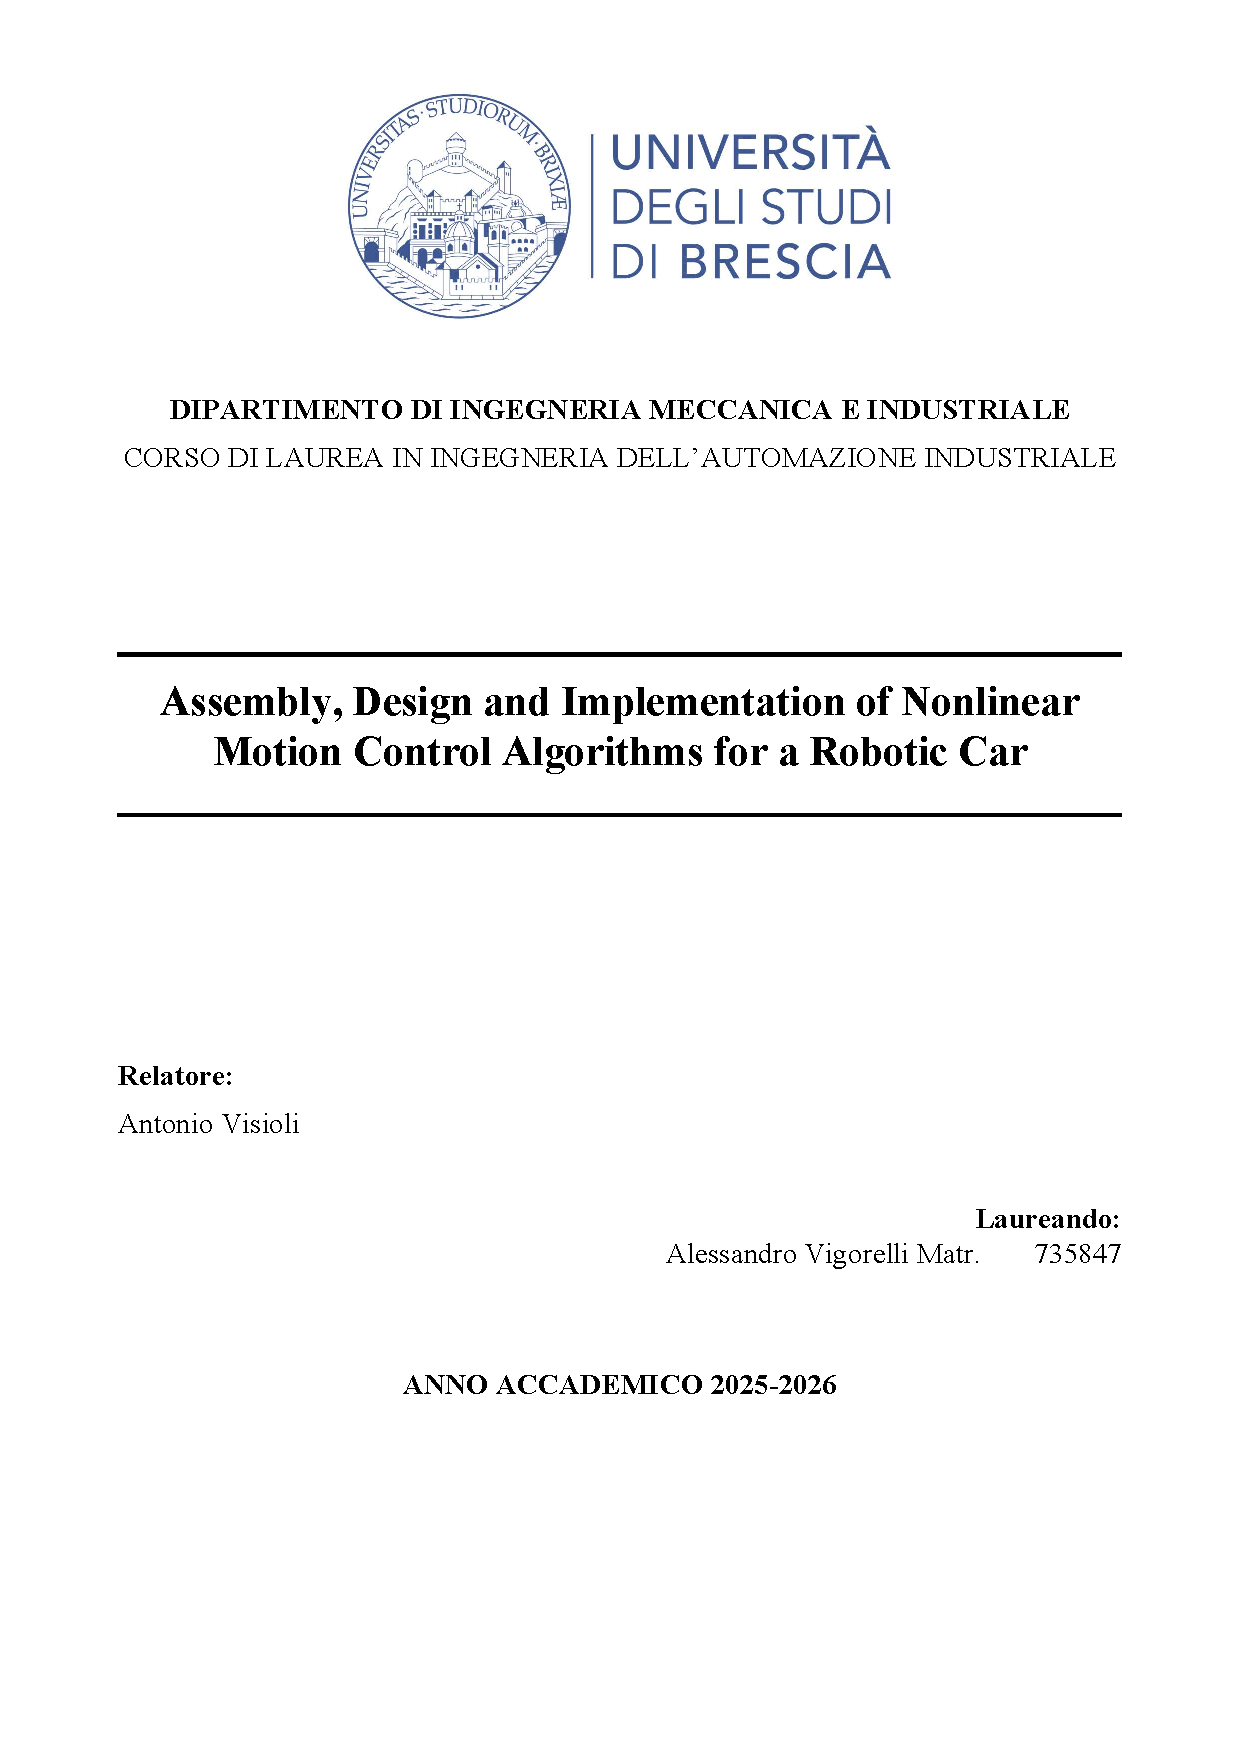
\includepdf[pages=-]{Frontespizio_TM.pdf} 

\tableofcontents 
\newpage

\pagenumbering{arabic}

% ESEMPIO DI UTILIZZO (Ora molto più sobrio)
% \begin{vscode}{main.cpp}
% #include <iostream>
% // Questo è un commento accademico
% int main() {
%     std::cout << "Stile Tesi Pulito" << std::endl;
%     return 0;
% }
% \end{vscode}

\chapter{Introduction}
\section{Problem Statement and Motivation}
Modern industrial automation is increasingly moving towards flexible and autonomous systems. Within this framework, omnidirectional robots represent a significant advancement due to their ability to move in any direction without altering their orientation.

This thesis documents the mechanical assembly, hardware architecture design, and implementation of nonlinear motion control algorithms for the \textbf{OMNICAR} platform. The robotic vehicle is designed to navigate autonomously within a workspace, optimizing both path planning and the associated control laws to ensure precision and efficiency.

\section{Maneuverability and Constraints}
Traditional differential drive robots face significant maneuverability challenges in confined industrial environments. This limitation stems from their mechanical design, which prevents the vehicle from moving sideways without first performing a rotation. 
In robotics, this physical restriction is classified as a \textbf{non-holonomic constraint}. Mathematically, this occurs when the number of controllable degrees of freedom is lower than the total degrees of freedom of the workspace. Consequently, these robots cannot follow any arbitrary trajectory instantaneously, often requiring complex maneuvers to navigate. This project addresses these issues by utilizing the \textbf{OMNICAR} platform, which allows for fluid and omnidirectional motion.

\section{Objectives and Contributions}
The primary focus of this research to date has been the complete redesign and physical realization of the OMNICAR platform. The specific objectives achieved during the initial phases of this work are:

\begin{itemize}
    \item \textbf{Mechanical Redesign and Optimization:} Utilizing Autodesk Fusion to completely overhaul the robot's structure. This involved increasing the chassis dimensions and implementing advanced design features to enhance structural integrity, usability, and internal layout.
    \item \textbf{Component Integration and Layout:} Designing custom mounts and optimized placements for the core hardware, including the Raspberry Pi 5, ESP32, LIDAR, Pi Camera, and MDD10A motor drivers, with a specific focus on sensor field-of-view and maintenance accessibility.
    \item \textbf{Electrical System Design:} Developing a comprehensive wiring schematic to define signal routing and pin mapping for the ESP32 microcontroller, ensuring a stable interface between the low-level logic and power electronics. Implementing cable management system like Wago connectors, custom soldering and routing solutions, to improve accessibility to system components.
    \item \textbf{Prototyping and Assembly:} Executing the 3D printing of structural components and the subsequent mechanical assembly of the two-layer chassis, integrating electronics.
\end{itemize}

Following the completion of the hardware phase, the next stages of this research will focus on the development of the real-time firmware, the implementation of control laws, and the final validation of the robot's navigation capabilities.
Following the completion of the hardware phase, the next stages of this research will focus on the development of the real-time firmware, the implementation of control laws, and the final validation of the robot's navigation capabilities.
\chapter{Hardware Design and System Architecture}

The OMNICAR platform is built upon a modular two-layer chassis, specifically designed to optimize the arrangement of sensors and processing units. 

Unlike traditional designs that strictly separate power and control electronics, this layout focuses on operational convenience and sensor efficiency. 

\begin{figure}[H]
    \centering
    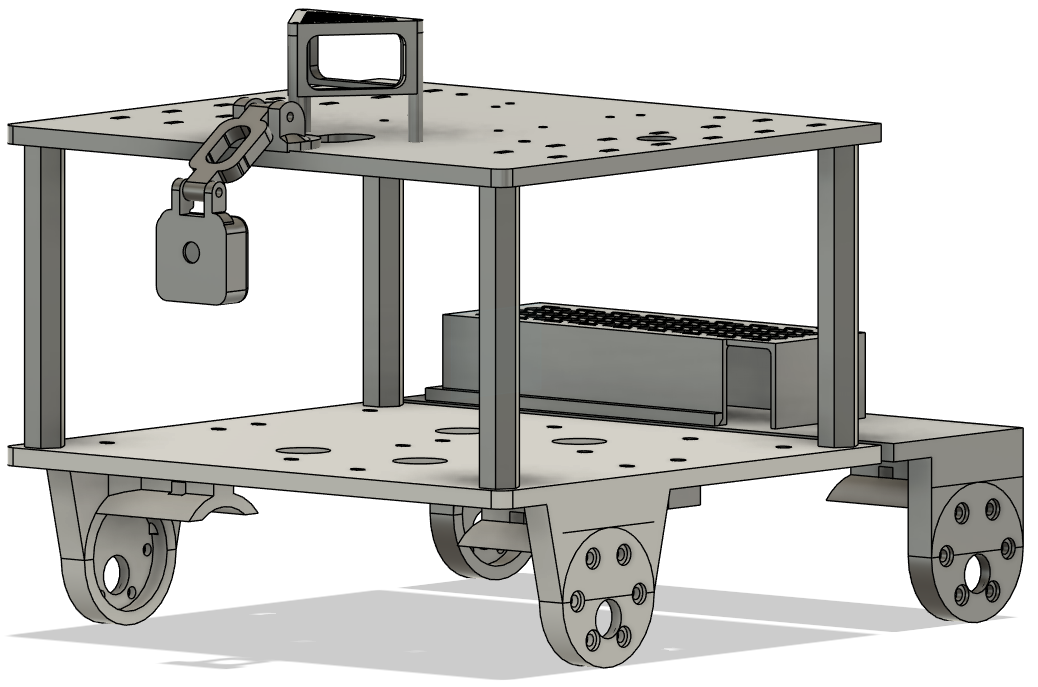
\includegraphics[width=0.8\textwidth]{IMG/Design/robot_completo.png}
    \caption{Full assembly model for 3D printing}
    \label{fig:primo_ordine}
\end{figure}

\newpage
\section{Mechanical Redesign and Optimization}
The \textbf{lower layer} houses the DC-DC converter, ESP32 microcontroller, motor drivers, and the battery, ensuring a low center of gravity for better dynamic stability. In this revision, the \textbf{motor mounts} have been significantly raised and reinforced to improve structural rigidity and better accommodate the mechanical stresses during high-torque maneuvers. Additionally, the mounts now feature dedicated slots for \textbf{nylon zip ties}, providing a secondary fastening method to ensure the motors remain perfectly aligned and secure. 

Furthermore, a custom \textbf{battery Case} has been designed and implemented. It utilizes a \textbf{sliding rail mechanism} that allows the Case to snap into place securely without the need for screws. This design choice significantly improves the robot's usability, allowing for rapid battery replacement during testing phases.

The \textbf{lower layer} houses the ESP32 microcontroller, motor drivers, and battery, keeping the center of mass low and reducing the wiring distance to the motors. 
% components of lower layer 
\begin{figure}[H]
    \centering
    \begin{minipage}[b]{0.4\textwidth}
        \centering
        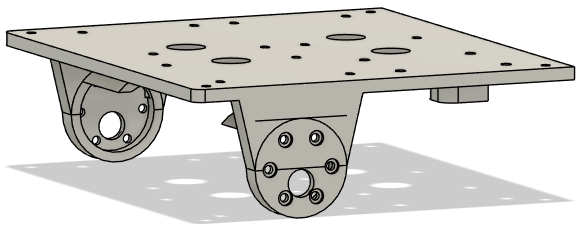
\includegraphics[width=\textwidth]{IMG/Design/ly1_front.png}
        \caption*{Front lower layer}
    \end{minipage}
    \hfill
    \begin{minipage}[b]{0.4\textwidth}
        \centering
        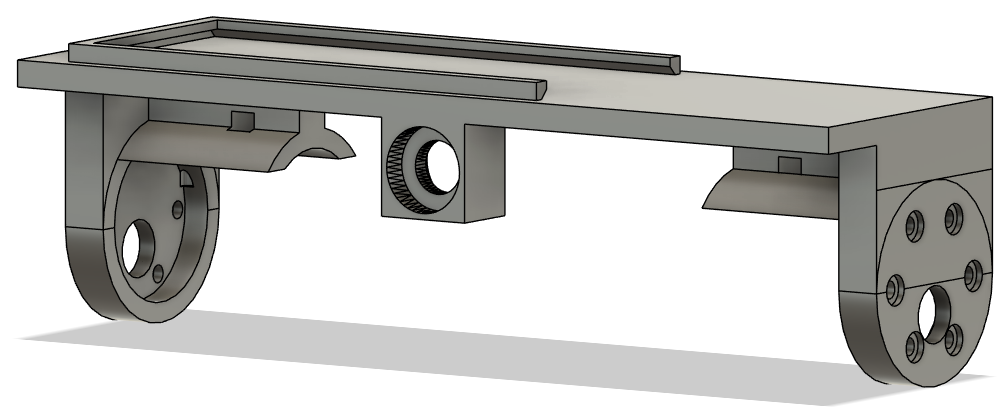
\includegraphics[width=\textwidth]{IMG/Design/ly1_back.png}
        \caption*{Back lower layer}
    \end{minipage}
    \hfill
    \begin{minipage}[b]{0.4\textwidth}
        \centering
        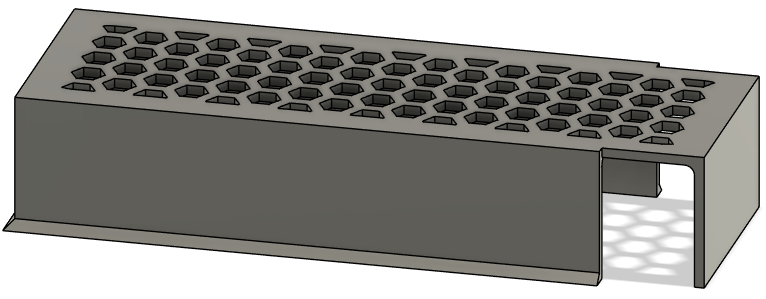
\includegraphics[width=\textwidth]{IMG/Design/cover_batteria.png}
        \caption*{Battery Case}
    \end{minipage}
    \caption{Lower layer components}
    \label{fig:Lower layer components}
\end{figure}

\begin{figure}[H]
    \centering
    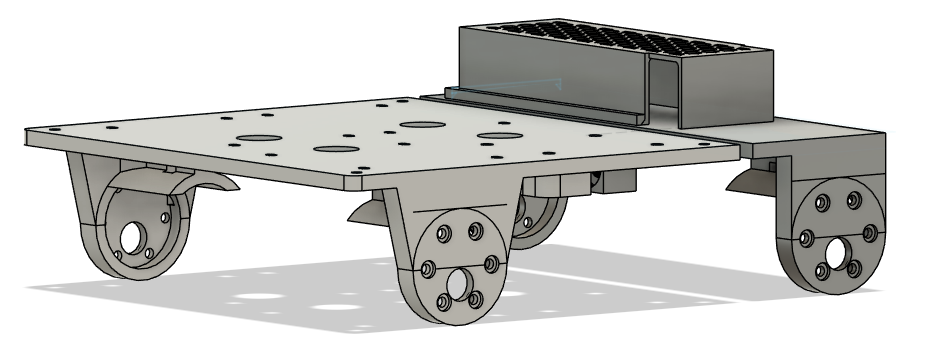
\includegraphics[width=0.7\textwidth]{IMG/Design/ly1_completo.png}
    \caption{Lower layer assembled}
    \label{fig:Lower layer assembled}
\end{figure}

\newpage
The \textbf{upper layer} is dedicated to the high-level navigation suite. It provides an elevated platform for the LIDAR and the Pi Camera, ensuring a clear line of sight for environment mapping and obstacle detection. Additionally, this placement allows the Raspberry Pi 5 to be located directly adjacent to the LIDAR, simplifying the USB/Serial connection and reducing electromagnetic interference in high-speed data transmission.

\begin{figure}[H]
    \centering
    \begin{minipage}[b]{0.60\textwidth}
        \centering
        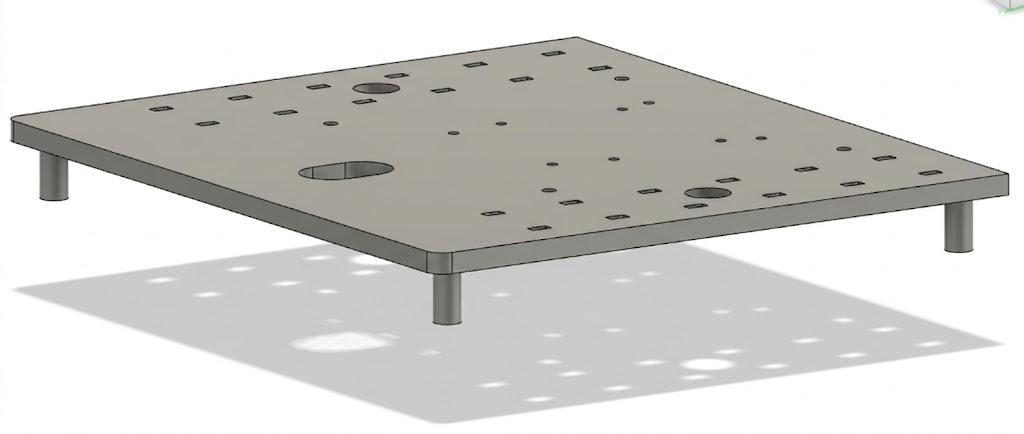
\includegraphics[width=\textwidth]{IMG/Design/ly2_piastra.jpg}
        \caption*{Upper layer}
    \end{minipage}
    \hfill
    \begin{minipage}[b]{0.28\textwidth}
        \centering
        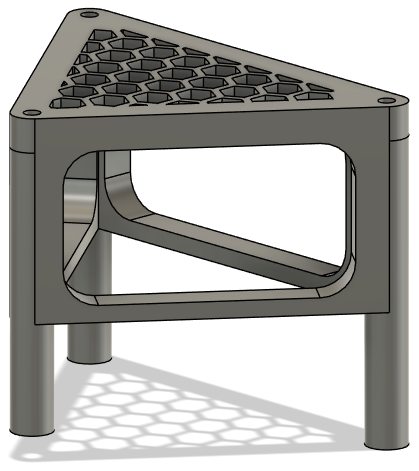
\includegraphics[width=\textwidth]{IMG/Design/lidar_support.png}
        \caption*{Lidar support}
    \end{minipage}
    \hfill
    \begin{minipage}[b]{0.28\textwidth}
        \centering
        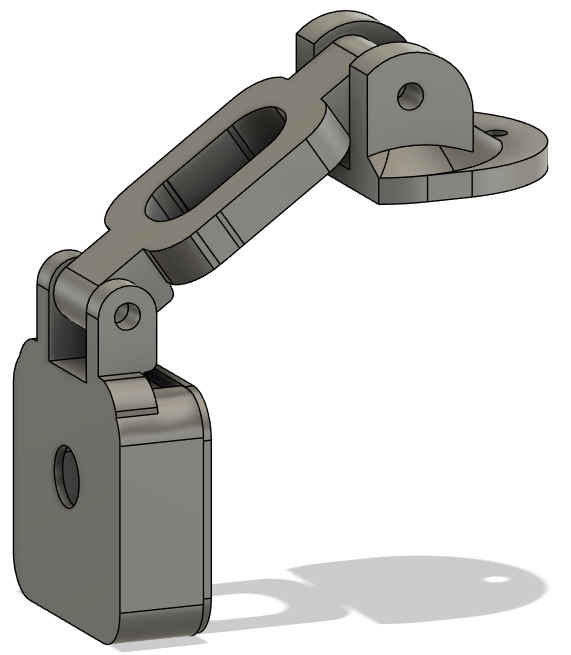
\includegraphics[width=\textwidth]{IMG/Design/stand_pi_camera.png}
        \caption*{Stand pi camera}
    \end{minipage}
    \caption{Upper layer components}
    \label{fig:Upper layer components}
\end{figure}


\begin{figure}[H]
    \centering
    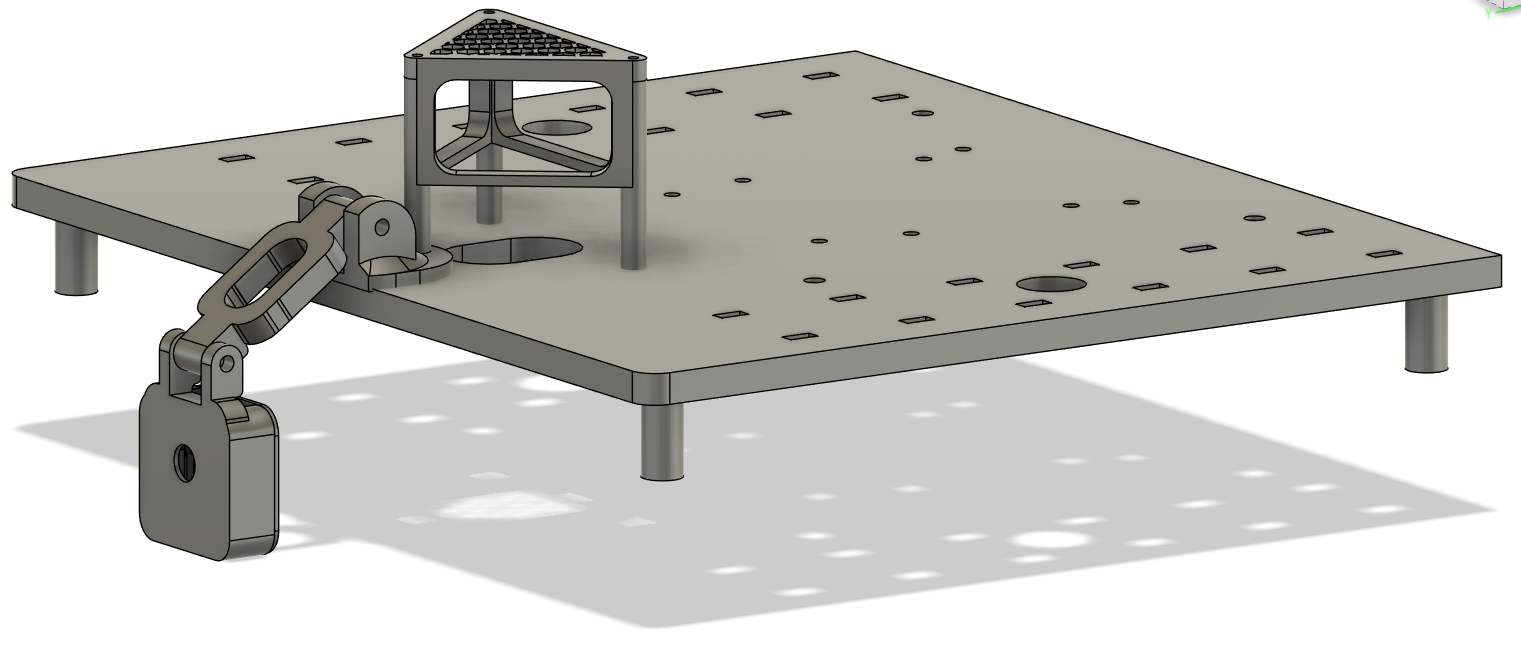
\includegraphics[width=0.7\textwidth]{IMG/Design/ly2_completo.png}
    \caption{Bottom layer assembled}
    \label{fig:Lower layer assembled}
\end{figure}

To facilitate the development and validation of the control algorithms, a custom-designed support stand was developed for the OMNICAR platform. This component proved to be \textbf{essential during the debugging and initial testing phases}, particularly for verifying the response of the four independent motors.

By elevating the chassis, the stand allowed the wheels to rotate freely in a "no-load" condition. 
This setup was extremely useful for:
\begin{itemize}
    \item Calibrating the high-resolution encoders without the interference of ground friction.
    \item Validating the mapping of PWM signals to the MDD10A motor drivers.
    \item Identifying potential hardware asymmetries or wiring issues before conducting field tests.
\end{itemize}

The mechanical design follows an \textbf{ergonomic and minimalist approach}. A key feature of the structure is the integration of a hollow central grip. This design choice was not only functional, providing an easy point of handle for moving the robot and stand together, but also strategically \textbf{economical}. By incorporating this empty space, the total volume of 3D-printing filament was significantly reduced, leading to faster production times and lower material costs without compromising the structural integrity required to support the robot's weight.

\begin{figure}[H]
    \centering
    \begin{minipage}[b]{0.48\textwidth}
        \centering
        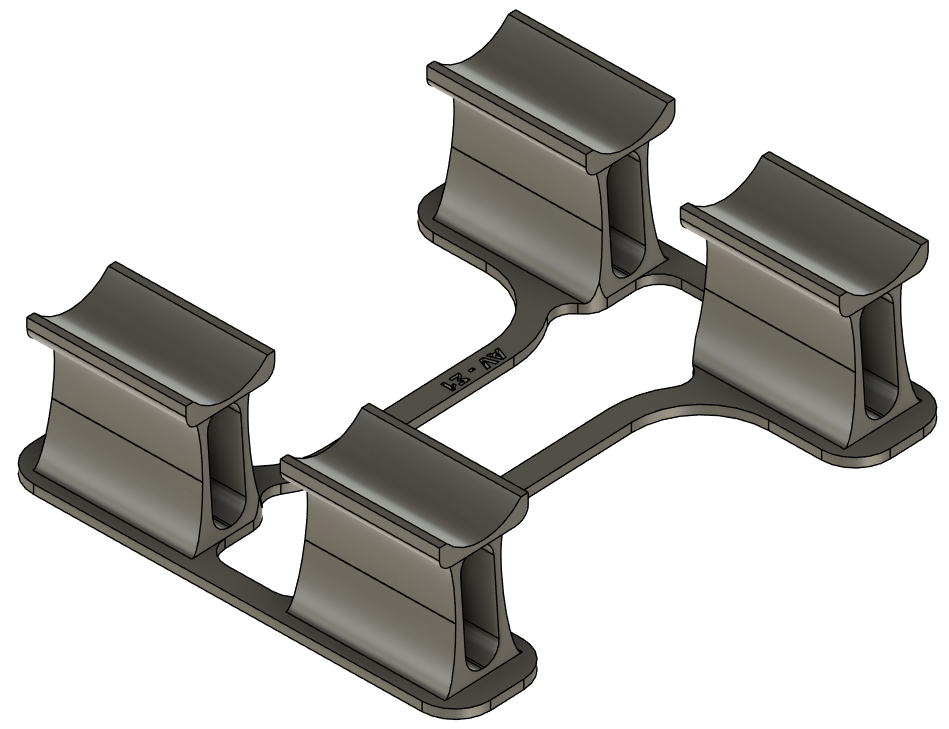
\includegraphics[width=\textwidth]{IMG/Design/Stand.png}
        \caption*{Stand}
    \end{minipage}
    \hfill
    \begin{minipage}[b]{0.48\textwidth}
        \centering
        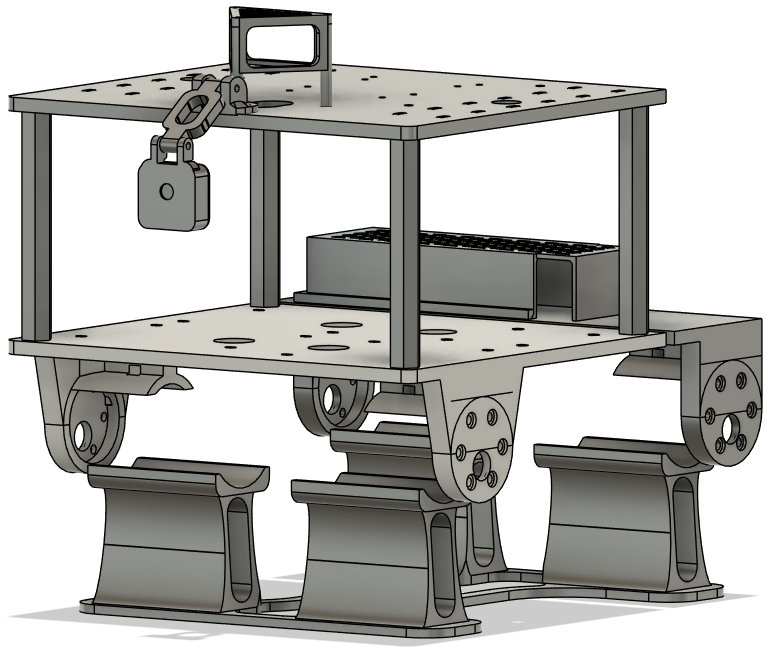
\includegraphics[width=\textwidth]{IMG/Design/Omnicar_with_Stand.png}
        \caption*{Omnicar and Stand assembled}
    \end{minipage}
    \label{fig:Omnicar and Stand assembled}
    \label{fig:Custom-designed test stand for the OMNICAR platform}
\end{figure}

\section{Actuators, Sensors and Electronic System}
The motion system is powered by four \textbf{Pololu 37Dx73L mm} metal gearmotors. These actuators are equipped with integrated 64 CPR quadrature encoders which, through the gear ratio, provide a high-resolution feedback of approximately \textbf{1200 counts per revolution}. This level of precision is fundamental for maintaining accurate odometry and ensuring stable trajectory tracking.

To manage the complex power requirements of both high-level processing and low-level actuation, the robot integrates a robust power distribution stage. A high-capacity \textbf{300W 20A DC-DC buck converter} is utilized to step down the battery voltage, providing a stabilized power rail for the most demanding components like encoders, \textbf{Raspberry Pi 5} and the \textbf{LIDAR} sensor.

To manage the complex power requirements of both high-level processing and low-level actuation, the robot's electrical architecture integrates a robust power distribution stage. The system is primary energized by a \textbf{Combo Battery 5000mAh 11.1V 3S1P} LiPo battery, chosen for its high energy density and discharge rate capabilities. To interface this source with the onboard electronics, a high-capacity \textbf{300W 20A DC-DC buck converter} is utilized to step down the battery voltage. This regulation provides a stabilized power rail for the most demanding components, including the high-resolution encoders, the \textbf{Raspberry Pi 5} central processing unit, and the \textbf{LIDAR} sensor, ensuring operational stability even during high-torque motor maneuvers.

\begin{figure}[H]
        \centering
        \begin{minipage}[b]{0.30\textwidth}
            \centering
            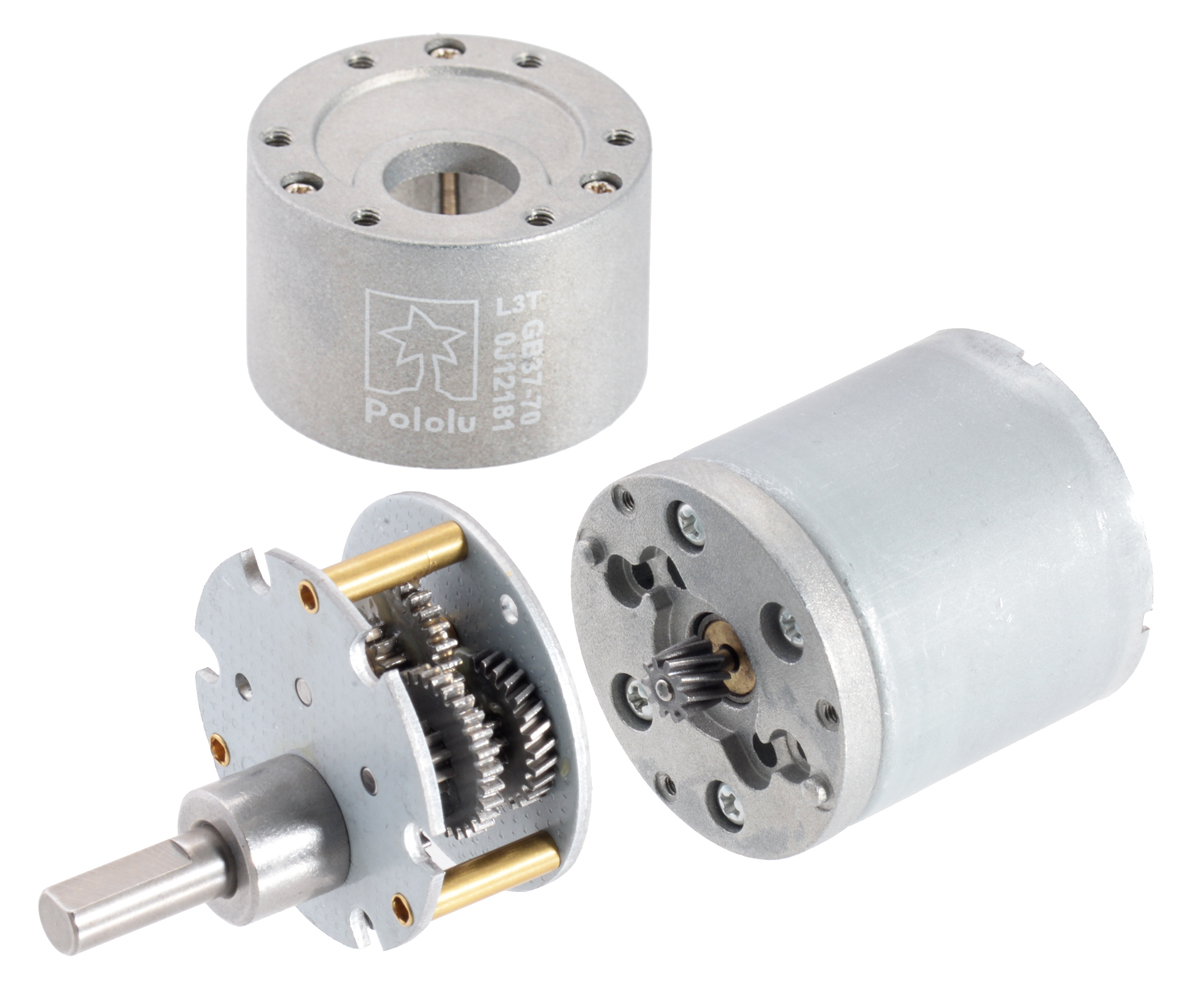
\includegraphics[width=\textwidth]{IMG/Componenti_Ele/pololu_motor.jpeg}
            \caption*{Pololu Metal DC Gearmotors}
        \end{minipage}
        \hfill
        \begin{minipage}[b]{0.30\textwidth}
            \centering
            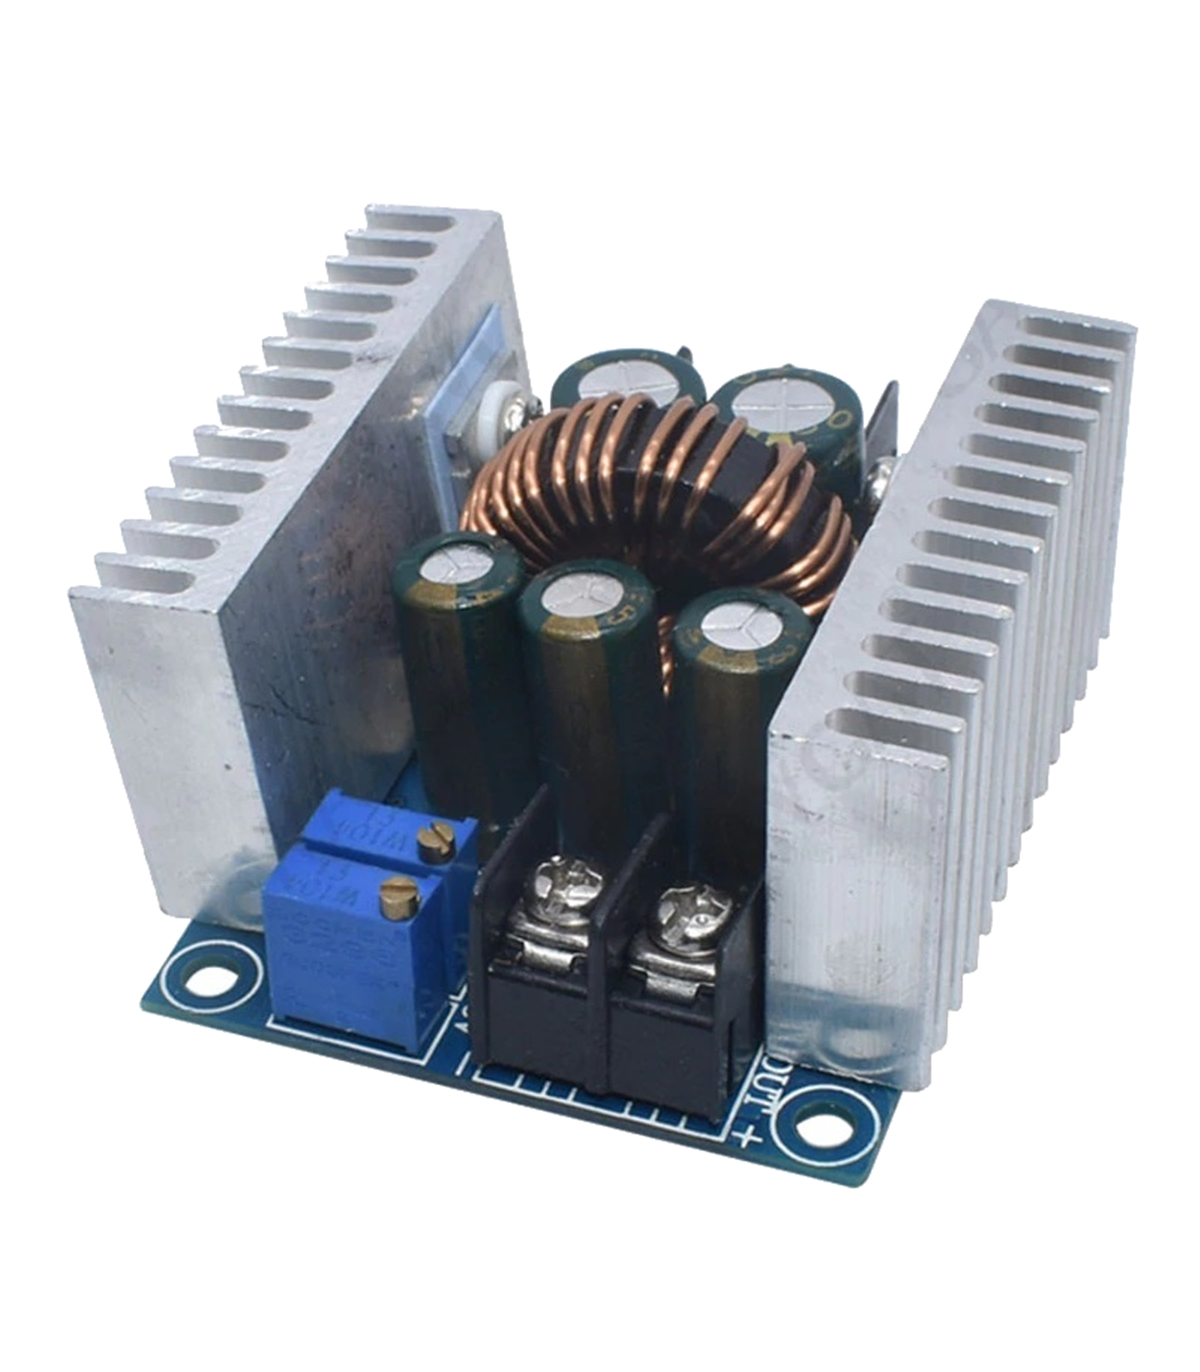
\includegraphics[width=\textwidth]{IMG/Componenti_Ele/DC_DC_Conv.jpg}
            \caption*{DC-DC Buck Converter }
        \end{minipage}
        \hfill
        \begin{minipage}[b]{0.50\textwidth}
            \centering
            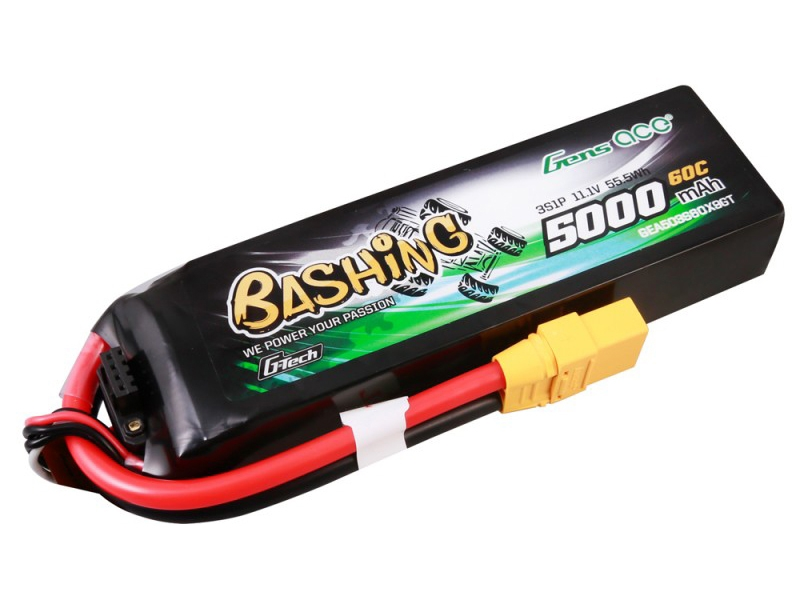
\includegraphics[width=\textwidth]{IMG/Componenti_Ele/battery_11_1.jpg}
    \caption{Battery 5000mAh 11.1V 3S1P}
        \end{minipage}
        \label{fig:12 Volt Components}
\end{figure}

\begin{comment}
\begin{figure}[H]
    \centering
    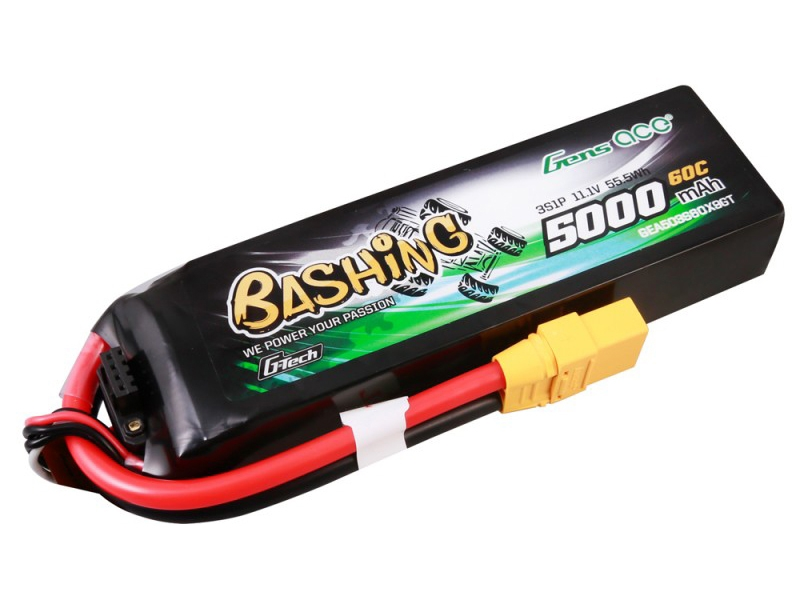
\includegraphics[width=0.40\textwidth]{IMG/Componenti_Ele/battery_11_1.jpg}
    \caption{Battery 5000mAh 11.1V 3S1P}
    \label{fig:Battery 5000mAh 11.1V 3S1P}
\end{figure}
\end{comment}

The control architecture is divided into two main functional blocks:

\begin{itemize}
    \item \textbf{Low-Level Control:} The core of this subsystem is an \textbf{ESP32-WROOM} microcontroller, chosen for its dual-core architecture and dedicated hardware peripherals. The ESP32 handles the real-time execution of the control loop, utilizing its hardware timers for precise \textbf{PWM generation} and its \textbf{Pulse Counter (PCNT)} modules for efficient, high-frequency encoder reading.
    
    \begin{figure}[H]
    \centering
    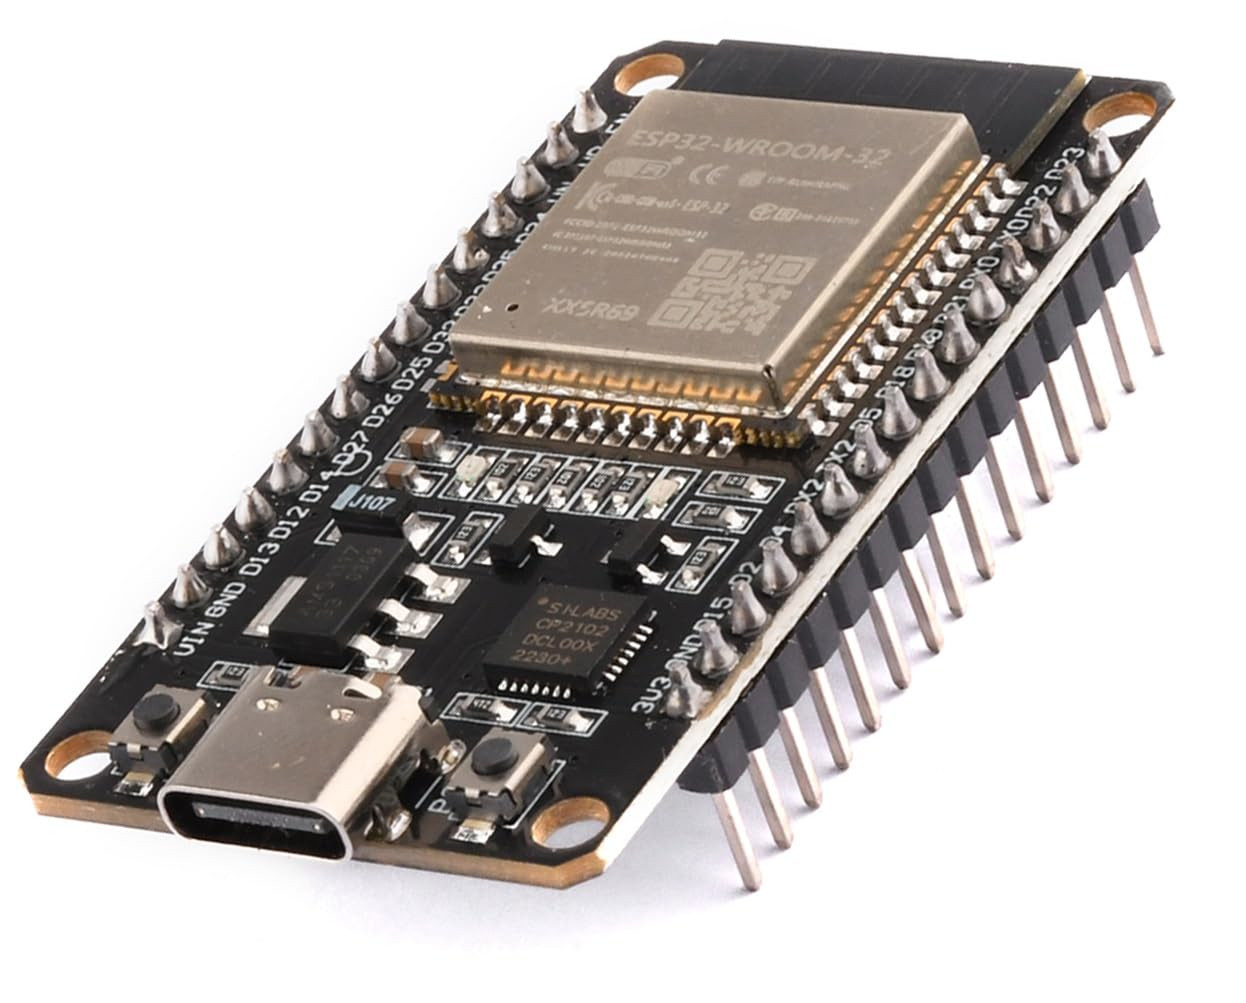
\includegraphics[width=0.45\textwidth]{IMG/Componenti_Ele/esp32.jpg}
    \caption{ESP32}
    \label{fig:ESP32}
    \end{figure}

    \item \textbf{Motor Actuation:} The microcontroller interfaces with two \textbf{MDD10A} dual-channel motor drivers. This setup allows for independent control of each wheel's speed and direction through a PWM/DIR interface, creating a closed-loop system where the ESP32 simultaneously commands the motors and monitors wheel position.
    
    \begin{figure}[H]
    \centering
    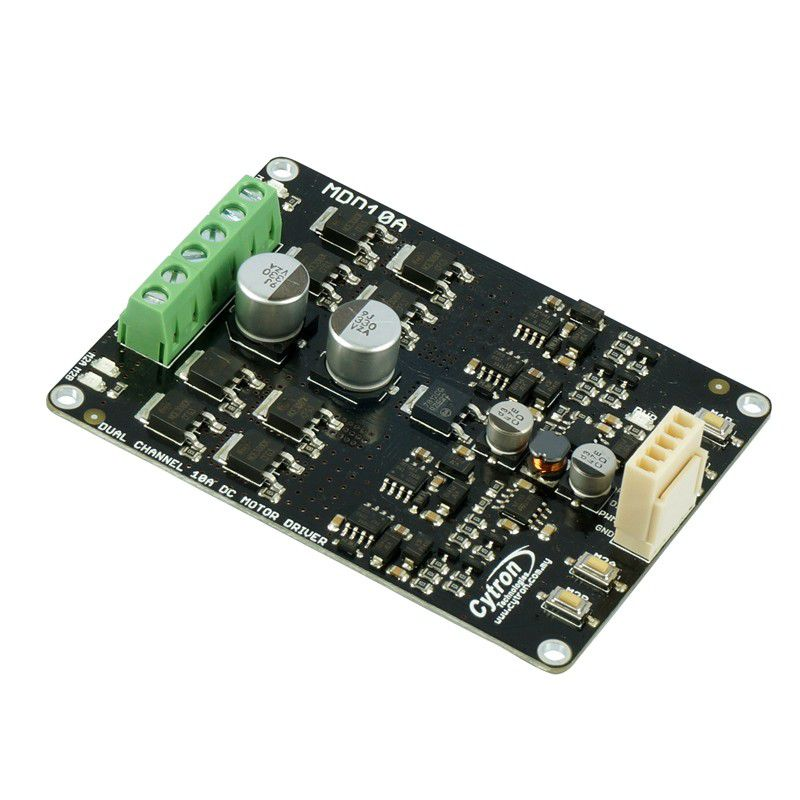
\includegraphics[width=0.45\textwidth]{IMG/Componenti_Ele/driver_MD10A.jpeg}
    \caption{Driver MDD10A}
    \label{fig:Driver MDD10A}
    \end{figure}
    
    \item \textbf{High-Level Navigation:} A \textbf{Raspberry Pi 5} serves as the primary computational unit, processing data from the \textbf{LIDAR} and \textbf{Pi Camera} to perform environment mapping and path planning, subsequently communicating target velocities to the ESP32.
    \begin{figure}[H]
        \centering
        \begin{minipage}[b]{0.43\textwidth}
            \centering
            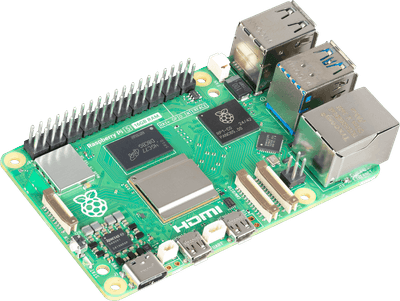
\includegraphics[width=\textwidth]{IMG/Componenti_Ele/raspberry_pi5.png}
            \caption*{Upper layer}
        \end{minipage}
        \hfill
        \begin{minipage}[b]{0.43\textwidth}
            \centering
            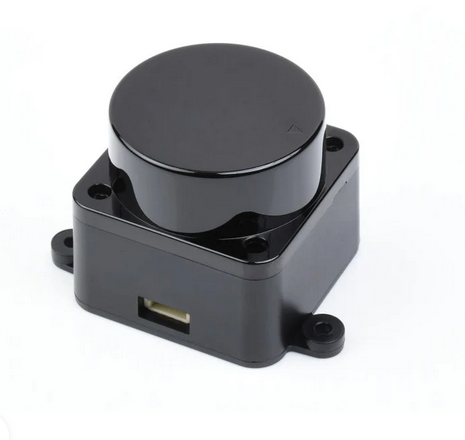
\includegraphics[width=\textwidth]{IMG/Componenti_Ele/Lidar.png}
            \caption*{Lidar}
        \end{minipage}
    \end{figure}
    
\end{itemize}

\section{Electrical Design and Connection Architecture}

The design of the entire electrical system for the OMNICAR platform was developed using the \textbf{EasyEDA online editor}. Thanks to the integrated component libraries, it was possible to model the power interfaces of the motor drivers and the logical connections of the microcontroller, ensuring a high degree of fidelity between the theoretical design and the final hardware.

The result of this phase is the \textbf{general electrical schematic} of the platform, illustrated in Figure \ref{fig:connection_architecture_easyeda}, which serves as the blueprint for the entire control and power distribution system. The schematic is structured to isolate the high-current power lines intended for the motors from the 3.3V and 5V logic signals required for the control logic and sensors. This separation is crucial to prevent cross-talk and ensure the stability of the feedback signals from the encoders during the robot's maximum acceleration phases.

\subsection{Physical Layout and Layer Organization}

The physical organization of the hardware follows a layered logic to optimize space and weight distribution:

\begin{itemize}
    \item \textbf{Lower Layer (Base):} This level constitutes the electromechanical heart of the robot. It houses the \textbf{ESP32 DevKit}, the four \textbf{MDD10A} drivers, and the power distribution system. Placing these at the base allows for a lower center of gravity and reduces the length of the wiring to the motors, minimizing electromagnetic interference (EMI).
    \item \textbf{Upper Layer (Sensor Deck):} To ensure a field of view free from obstacles, the \textbf{Raspberry Pi 5}, the \textbf{LIDAR} sensor, and the \textbf{Pi Camera} are installed on the upper structure. This configuration protects the processing units from the heat generated by the drivers and provides an optimal perspective for navigation and vision algorithms.
\end{itemize}

\subsection{ESP32 Pinout and Wiring Specification}

The \textbf{ESP32-WROOM} microcontroller was selected for its high-performance architecture, capable of simultaneously managing non-linear control loops and high-frequency encoder readings. The connection configuration was designed to maximize the use of dedicated hardware peripherals, such as PWM (LEDC) and Pulse Counters (PCNT). The detailed mapping of these connections is provided in Table \ref{tab:esp32_pinout}.

\subsection{Pin Selection Justification}

The pin assignment was guided by specific technical constraints to ensure system reliability:

\begin{enumerate}
    \item \textbf{High-Resolution Feedback:} With encoders providing 1200 pulses per revolution, it was necessary to use pins compatible with the \textbf{PCNT} hardware peripheral. Pins 34-39 were specifically chosen for the rear encoders because, as "Input-Only" pins, they lack internal pull-up/pull-down circuitry that could interfere with the signal, thus guaranteeing digital integrity without the risk of output conflicts.
    \item \textbf{PWM Generation:} The \textbf{LEDC} peripheral was utilized to control the MDD10A drivers. The assigned pins allow for independent, hardware-timed PWM signals, which are essential for maintaining a deterministic response in holonomic kinematics.
    \item \textbf{Communication Integrity:} Predefined hardware \textbf{UART} pins were reserved for data exchange with the Raspberry Pi 5, supporting baud rates up to 115200 bps for real-time transmission of velocities and poses.
\end{enumerate}

\begin{comment}
    \item \textbf{Boot Stability:} So-called "strapping pins" (such as GPIO 0, 2, 5, 12, and 15) and pins linked to the internal SPI flash were avoided where possible to prevent firmware boot errors or unexpected behavior during power-up under full-load conditions.
\end{comment}

% --- Final Figures and Tables ---
\begin{table}[H]
\centering
\caption{ESP32 Complete Pinout for OMNICAR Motion Control}
\label{tab:esp32_pinout}
% Definiamo un colore leggero per le righe alternate (grigio al 90% di bianco)
\rowcolors{2}{gray!10}{white} 
\begin{tabularx}{\textwidth}{l c c X} % X è una colonna che si espande automaticamente
\toprule
\textbf{Function} & \textbf{GPIO} & \textbf{Signal Type} & \textbf{Project Description} \\ 
\midrule
Main Power Supply & VIN & Power (+5V) & Main DC input \\
Common Ground     & GND & GND          & Common return \\
\addlinespace % Piccolo spazio extra per separare i gruppi
Motor FL PWM      & 13  & Output (LEDC) & Front-Left speed control \\
Motor FL DIR      & 12  & Output        & Front-Left direction \\
Motor FR PWM      & 14  & Output (LEDC) & Front-Right speed control \\
Motor FR DIR      & 27  & Output        & Front-Right direction \\
Motor RL PWM      & 26  & Output (LEDC) & Rear-Left speed control \\
Motor RL DIR      & 25  & Output        & Rear-Left direction \\
Motor RR PWM      & 33  & Output (LEDC) & Rear-Right speed control \\
Motor RR DIR      & 32  & Output        & Rear-Right direction \\
\addlinespace
Encoder FL (A/B)  & 16 / 17 & Input (PCNT) & Front-Left feedback \\
Encoder FR (A/B)  & 5 / 18 & Input (PCNT) & Front-Right feedback \\
Encoder RL (A/B)  & 19 / 21 & Input (Only) & Rear-Left feedback \\
Encoder RR (A/B)  & 22 / 23 & Input (Only) & Rear-Right feedback \\
\bottomrule
\end{tabularx}
\end{table}

\newgeometry{margin=3cm} % Stringe i margini solo per questa pagina
\begin{figure}[p]
    \centering
    \vspace*{\fill}
    \makebox[\textwidth][c]{%
        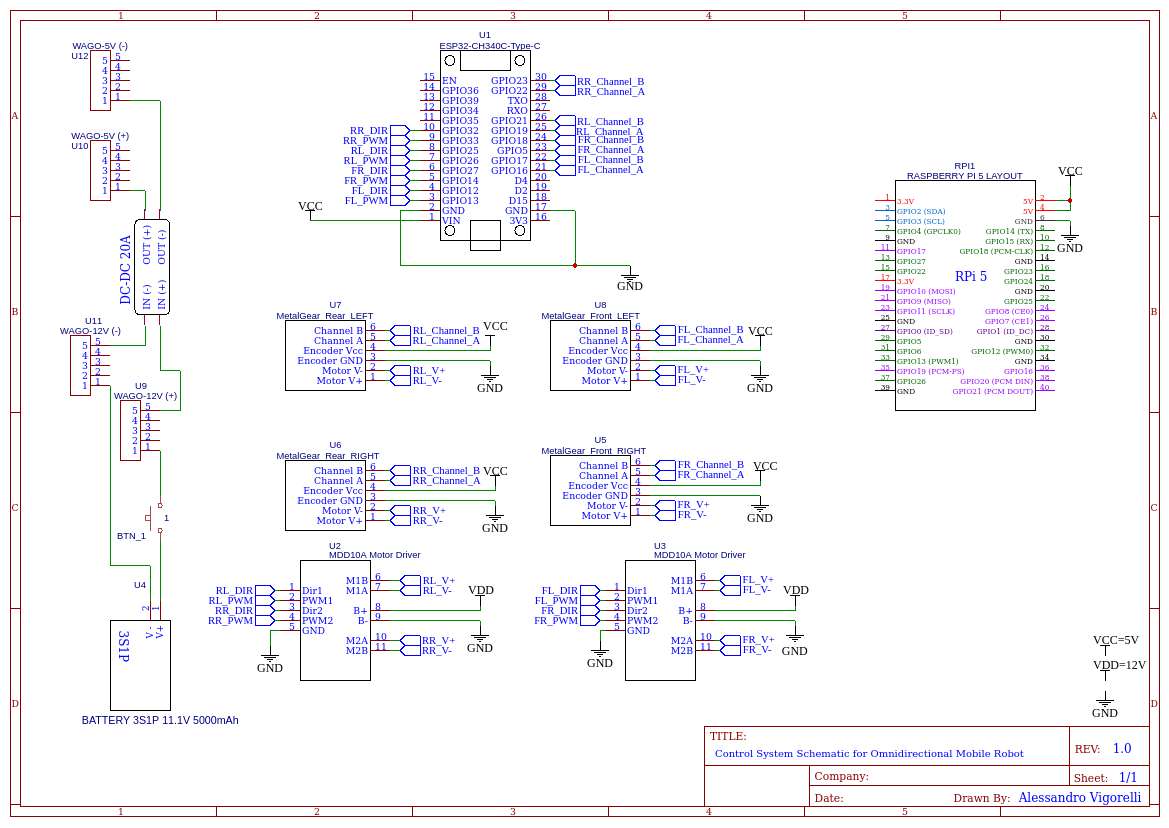
\includegraphics[height=1.1\textwidth, angle=90, origin=c]{IMG/Design/Schematic_OMNICAR.png}
    }
    \vspace*{\fill}
    \caption{Detailed Connection Architecture designed in EasyEDA}
    \label{fig:connection_architecture_easyeda}
\end{figure}
\restoregeometry % Torna ai margini normali nella pagina successiva
\chapter{Physical Implementation and Assembly}

This chapter details the transition from the digital design environment to the physical realization of the OMNICAR platform. The process encompasses the additive manufacturing of the structural components, the integration of the power electronics, and a rigorous multi-stage assembly and validation workflow.

\section{Additive Manufacturing: 3D Printing Phase}

The structural integrity of OMNICAR is primarily based on components manufactured through Fused Deposition Modeling (FDM). All custom parts were produced using a \textbf{Prusa MK3S+} 3D printer, known for its reliability and dimensional accuracy. 

The material selected for the entire chassis and support system was \textbf{PLA (Polylactic Acid)}, chosen for its ease of printing, rigidity, and minimal warping. To balance structural strength with weight optimization, a standard \textbf{infill density of 15\%} was applied to most components. However, for the primary structural elements—specifically the \textbf{Layer 1 Front}, \textbf{Layer 1 Back}, and \textbf{Layer 2}—the infill was increased to 25\% to ensure higher mechanical resistance to the stresses generated by the four DC motors and the overall payload.

\subsection{Printing Statistics and Material Consumption}

The manufacturing process was planned to optimize time and material usage. Table \ref{tab:printing_stats} summarizes the printing time and material consumption (in grams) for the main structural modules, as derived from the G-code analysis.

\begin{table}[H]
\centering
\caption{OMNICAR 3D Printing Parameters and Statistics}
\label{tab:printing_stats}
\rowcolors{2}{gray!10}{white}
\begin{tabularx}{\textwidth}{X c c c}
\toprule
\textbf{Component} & \textbf{Printing Time} & \textbf{Material [g]} & \textbf{Infill [\%]} \\ 
\midrule
Layer 1 Front               & 11h 54m & 115g & 25\% \\
Layer 1 Back                & 9h 47m  & 95g  & 25\% \\
Layer 2                     & 6h 41m  & 70g  & 25\% \\
Battery Case and Support    & 7h 11m  & 55g  & 15\% \\
Structural Pillars (Set)    & 6h 29m  & 88g  & 15\% \\
Stand                       & 19h 44m & 160g & 15\% \\
\midrule
\textbf{TOTAL}              & \textbf{61h 46m} & \textbf{583g} & \textbf{---} \\
\bottomrule
\end{tabularx}
\end{table}

\begin{figure}[H]
    \centering
    \begin{minipage}[b]{0.49\textwidth}
        \centering
        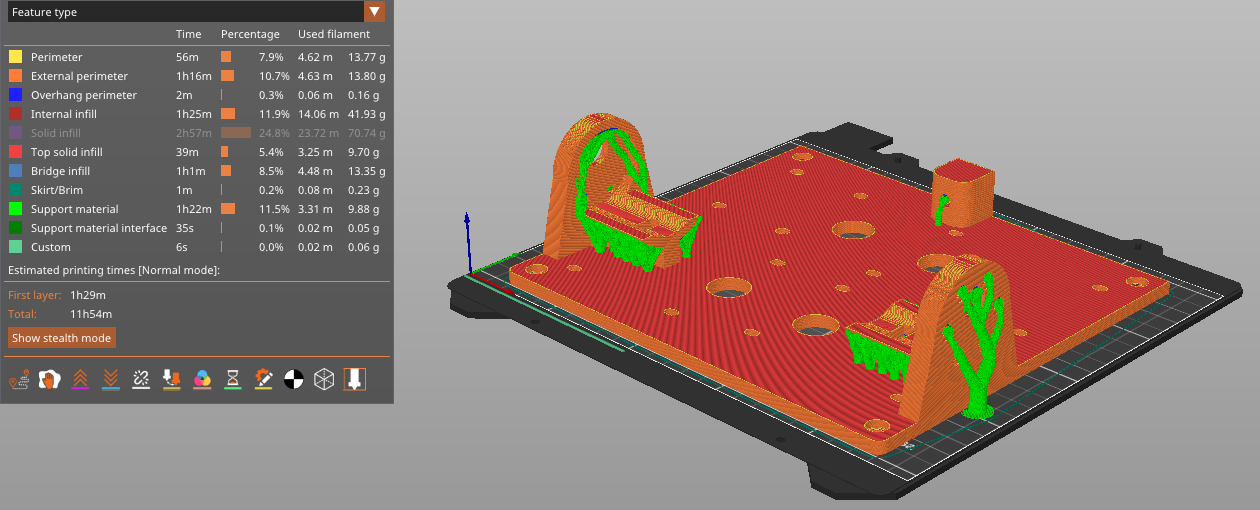
\includegraphics[width=\textwidth]{IMG/PrusaSlicer/prusa_ly1_front.png}
        \caption*{Front lower layer}
    \end{minipage}
    \hfill
    \begin{minipage}[b]{0.49\textwidth}
        \centering
        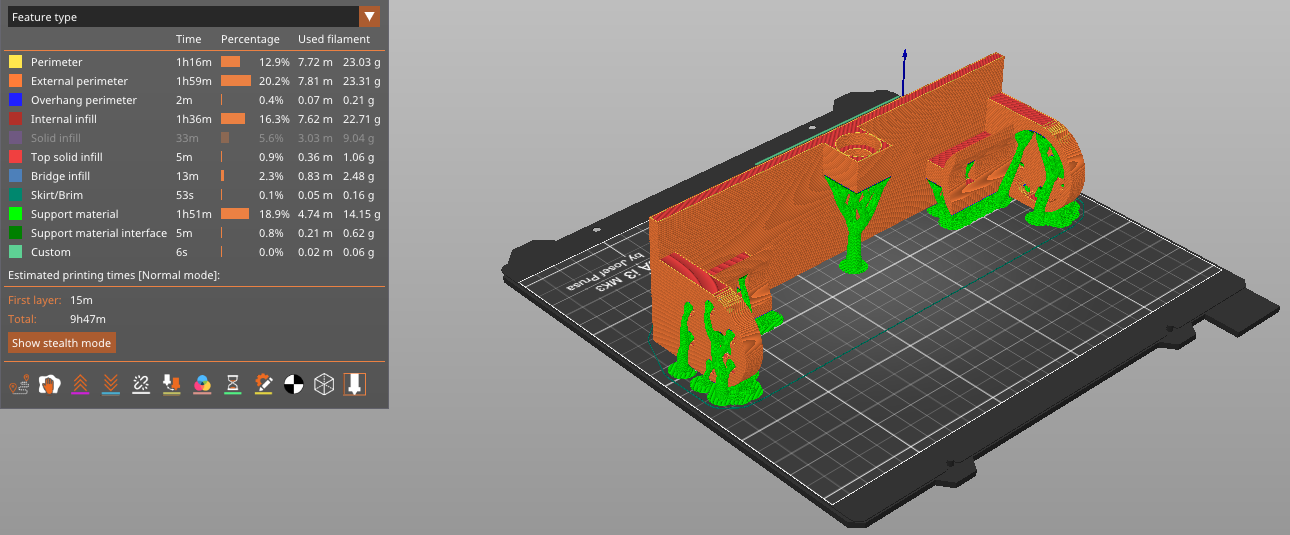
\includegraphics[width=\textwidth]{IMG/PrusaSlicer/prusa_ly1_back.png}
        \caption*{Back lower layer}
    \end{minipage}

    \vspace{1em} 

    \begin{minipage}[b]{0.49\textwidth}
        \centering
        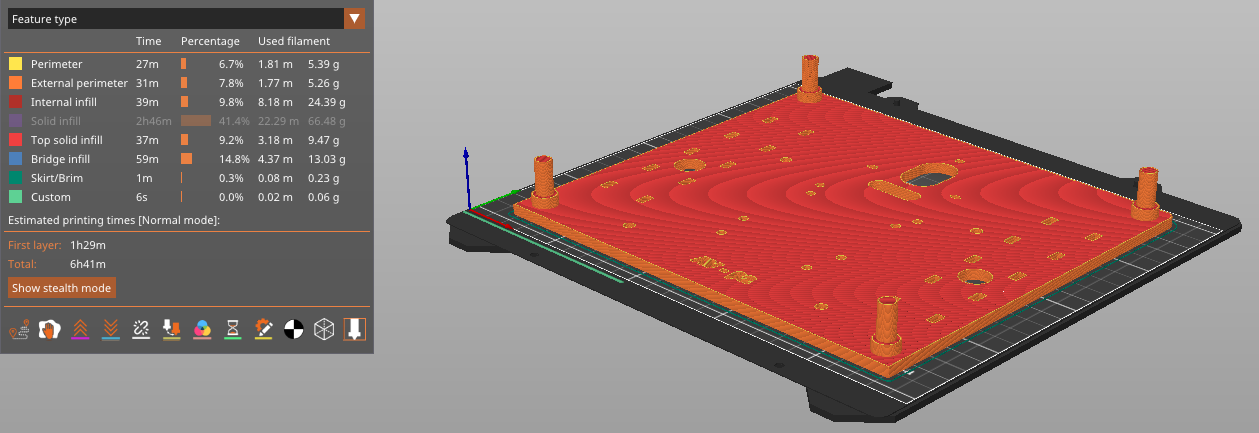
\includegraphics[width=\textwidth]{IMG/PrusaSlicer/prusa_ly2.png}
        \caption*{Upper Layer}
    \end{minipage}
    \hfill
    \begin{minipage}[b]{0.49\textwidth}
        \centering
        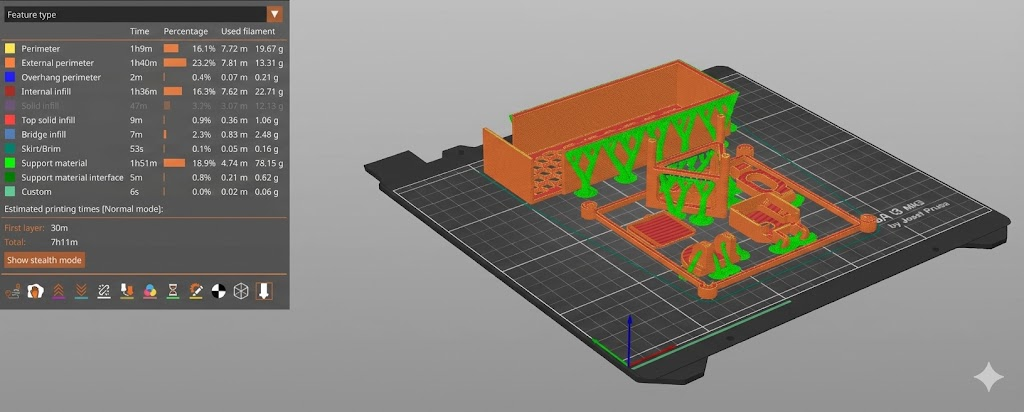
\includegraphics[width=\textwidth]{IMG/PrusaSlicer/Batteria_cover_and_supporti.jpg}
        \caption*{Battery Case and Supports}
    \end{minipage}

    \vspace{1em} 

    \begin{minipage}[b]{0.49\textwidth}
        \centering
        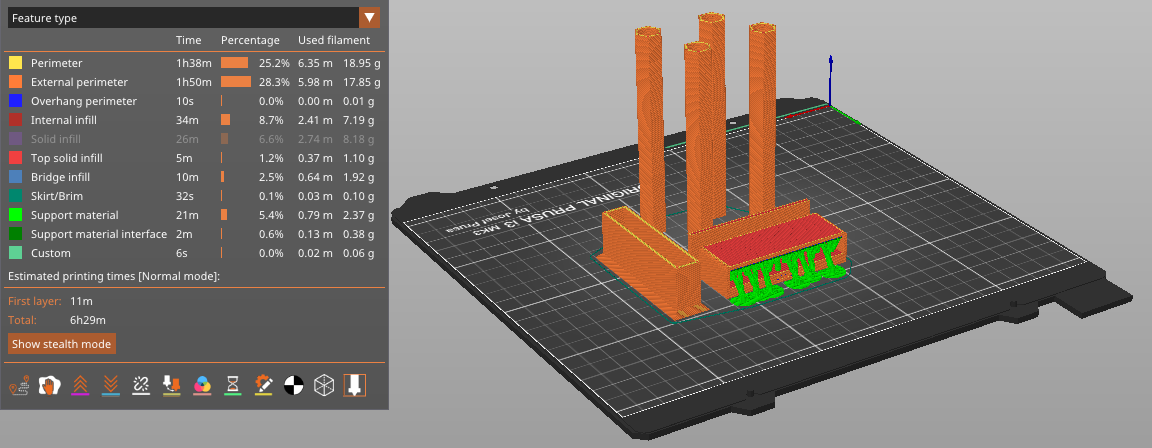
\includegraphics[width=\textwidth]{IMG/PrusaSlicer/prusa_pillar_wago.png}
        \caption*{Structural pillars and Wago Case}
    \end{minipage}
    \hfill
    \begin{minipage}[b]{0.49\textwidth}
        \centering
        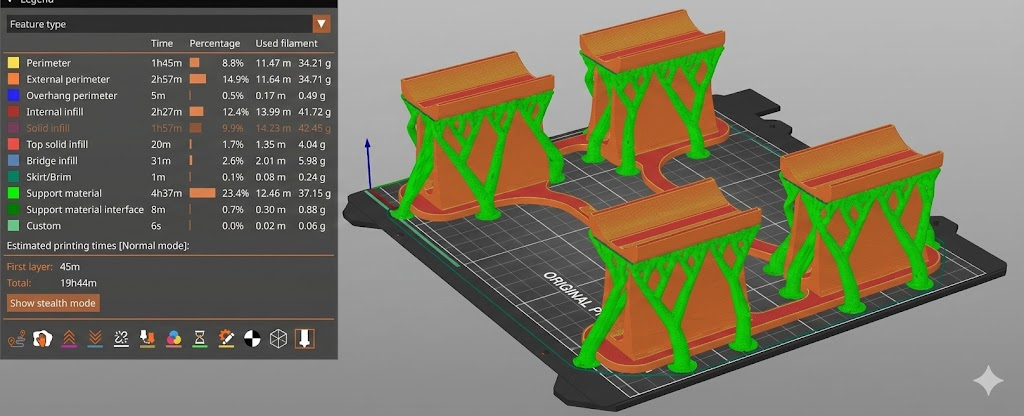
\includegraphics[width=\textwidth]{IMG/PrusaSlicer/Stand_support.jpg}
        \caption*{Robot Test Stand}
    \end{minipage}

    \caption{Slicing preview of OMNICAR components in PrusaSlicer}
    \label{fig:Slicing_preview}
\end{figure}

\section{Mechanical Assembly}

The robot's construction follows a modular "bottom-up" methodology, designed to optimize internal volume distribution and ensure high maintainability. The structure is organized into two primary functional layers connected by rigid vertical pillars.

\subsection{Layer 1: Traction and Power Distribution}
The lower deck (Layer 1) serves as the structural foundation and houses the high-power components. During the initial assembly phase, the motors and core components were positioned without wiring to verify dimensional fits (Figure \ref{fig:physical_assembly_steps}).
\begin{itemize}
    \item \textbf{Suspension and Chassis Coupling:} The connection between the front and rear sections is achieved through a structural bolt passing through flanged bearings. This assembly creates a pivot point that acts as a passive suspension system, allowing the frame to adapt to surface irregularities.
    \item \textbf{Actuation System:} Motor leads were extended by soldering custom wires insulated with heat-shrink tubing to reach the drivers efficiently.
\end{itemize}

\subsection{Power Management: DC-DC Conversion}
To provide a stable logic supply, a \textbf{DC-DC 9A 300W Step-Down Buck Converter} was integrated. The module was calibrated by adjusting its internal multi-turn potentiometer. Although the nominal target was 5.2V to compensate for voltage drops under load, the tuning phase was critical to ensure the Raspberry Pi 5 receives a consistent voltage within its operational tolerances.

\subsection{Layer 2: Logic and Navigation}
The electronics deck (Layer 2) isolates sensitive logic components from electromagnetic interference (EMI). 
\begin{itemize}
    \item \textbf{Processing Unit:} The \textbf{Raspberry Pi 5} is mounted as the central controller.
    \item \textbf{Sensors:} The \textbf{Pi Camera} and \textbf{Lidar} provide an unobstructed $360^{\circ}$ field of view.
\end{itemize}

\begin{figure}[H]
    \centering
    \begin{minipage}[b]{0.40\textwidth}
        \centering
        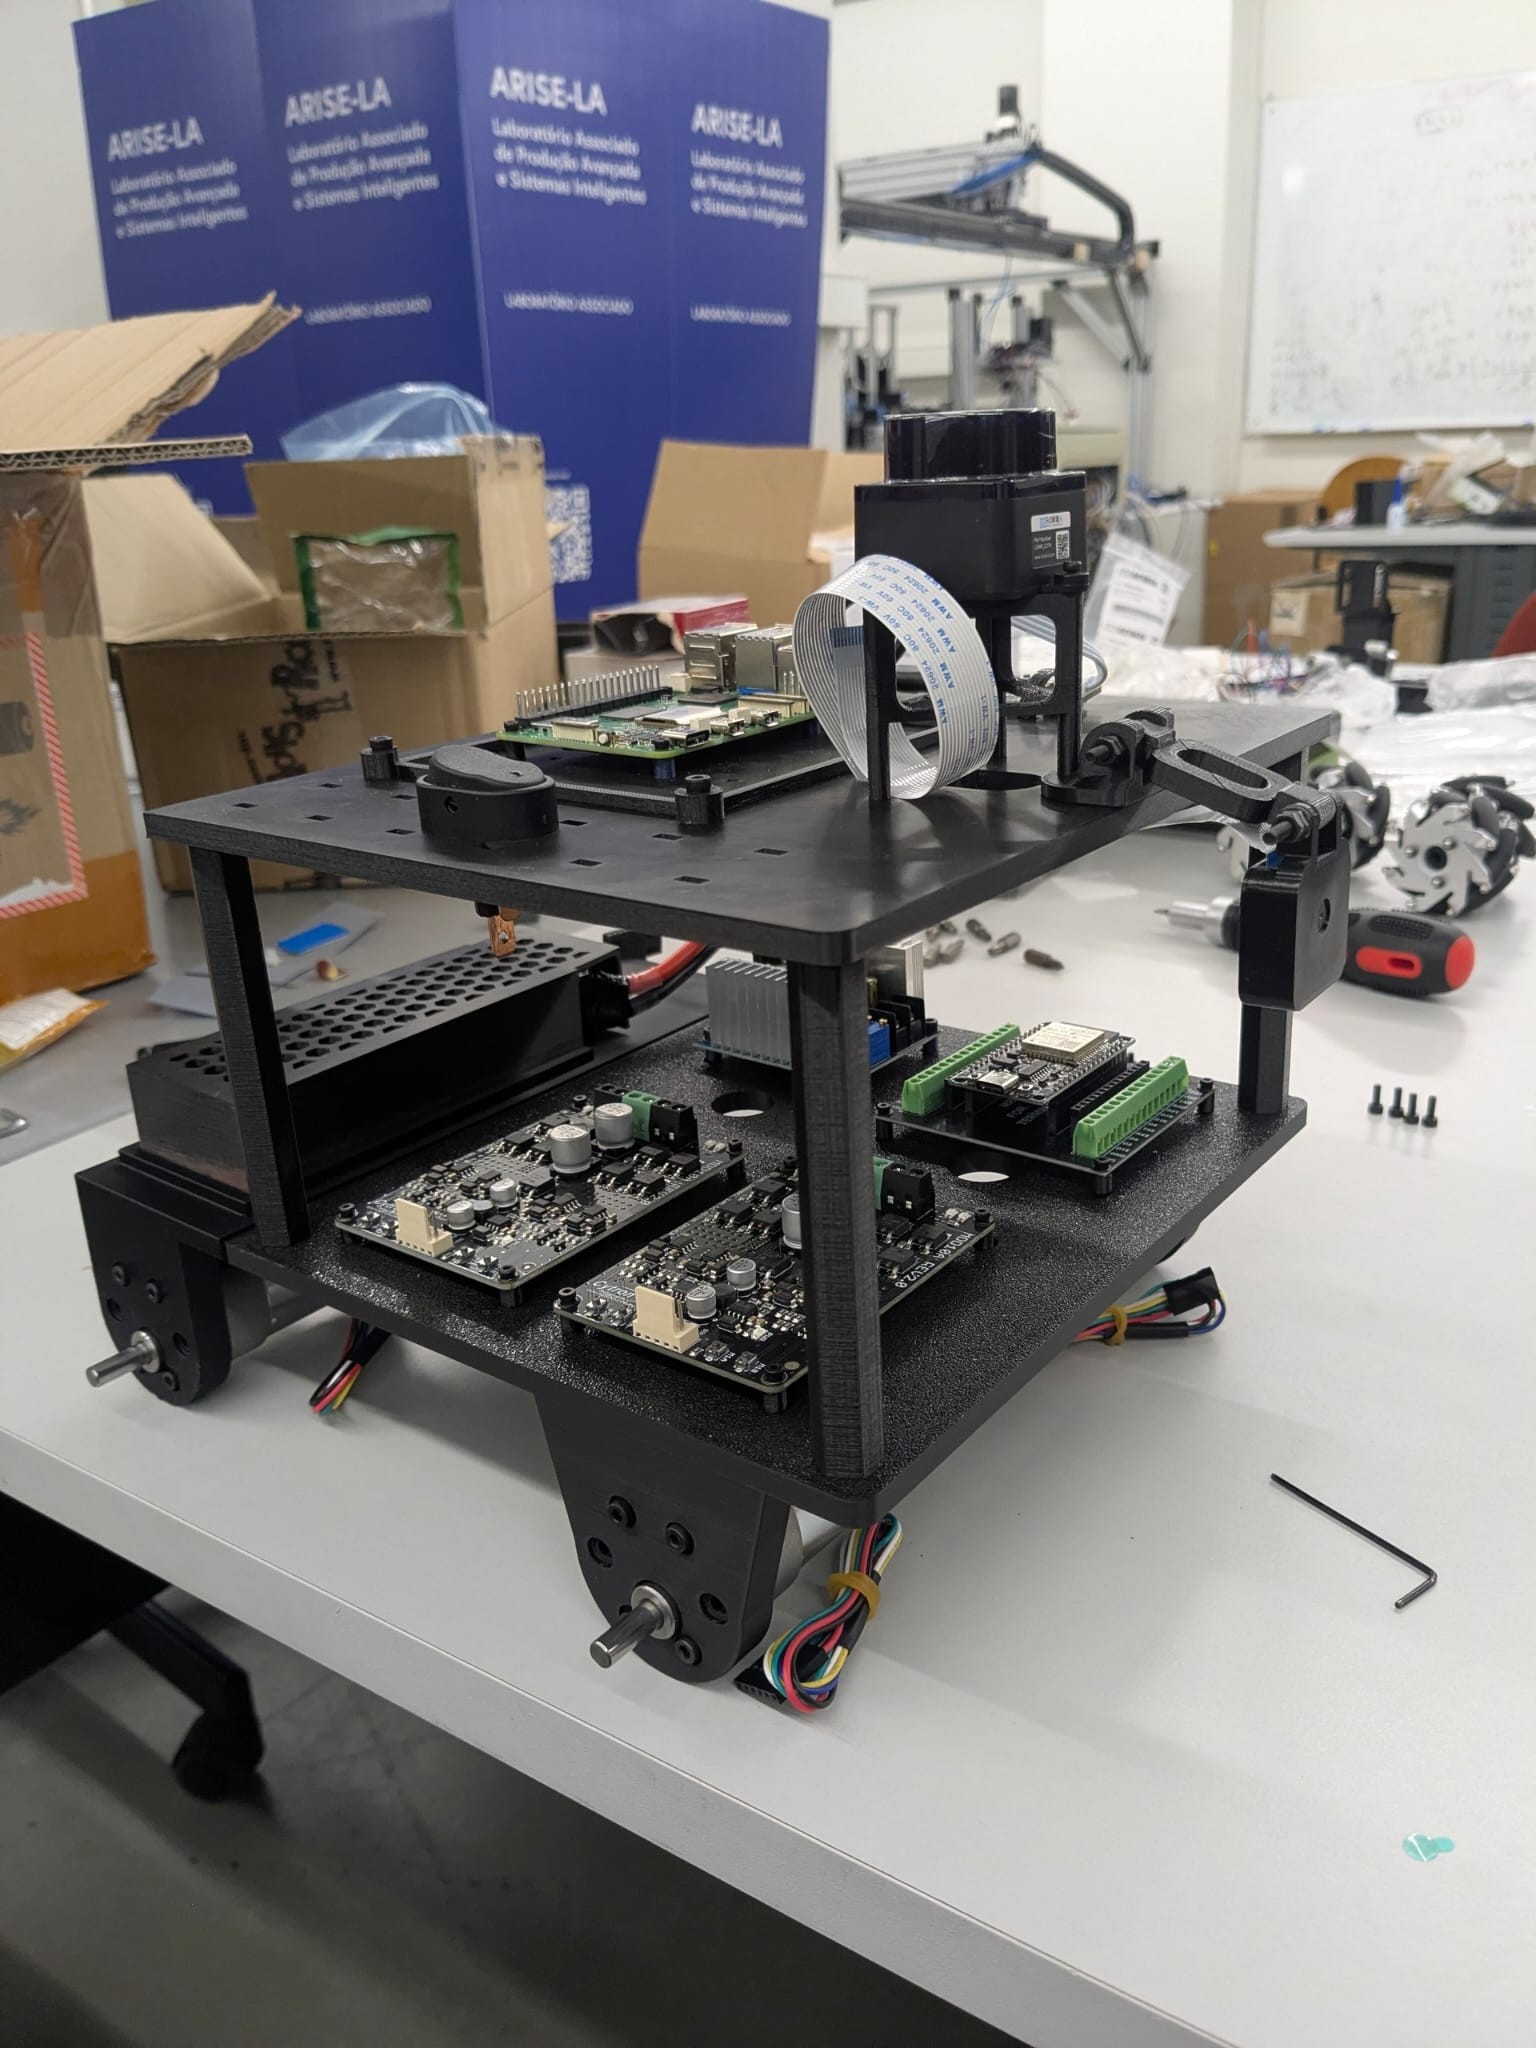
\includegraphics[width=\textwidth]{IMG/Real/Real_omnicar_beta.jpg}
        \caption*{Robot without wiring}
    \end{minipage}
    \hfill
    \begin{minipage}[b]{0.55\textwidth}
        \centering
        \includegraphics[width=\textwidth]{IMG/Real/Real_omnicar_section.jpg}
        \caption*{Main component in the lower layer}
    \end{minipage}
    \caption{Physical assembly of the OMNICAR lower layer}
    \label{fig:physical_assembly_steps}
\end{figure}

\section{Assembly Workflow and System Validation}

The implementation followed a rigorous chronological sequence to minimize the risk of electrical failure and ensure the correctness of the low-level control loops.

\subsection{Wiring and Electrical Pre-testing}
Following the layout of Layer 1 and Layer 2, the wiring was executed according to the previously defined electrical schematic. The circuit was powered by the LiPo battery, and the \textbf{DC-DC converter tuning} was performed as the first step.

The motor actuation was validated by connecting the motors to the MDD10A drivers and supplying 12V for power and 5V for logic. Initial functionality was confirmed \textbf{manually} via the physical test buttons on the drivers, ensuring the gearmotors responded correctly before involving the microcontroller. Subsequently, the DIR and PWM signal lines were routed to the \textbf{ESP32}.

\subsection{Firmware Configuration and Signal Analysis}
A preliminary firmware was developed using \textbf{PlatformIO} to test the PWM generation. As illustrated in Figure \ref{fig:pwm_signal}, the ESP32 successfully generated a stable square wave with a 50\% duty cycle, confirming the correct configuration of the LEDC hardware peripherals.


\begin{figure}[H]
    \centering
    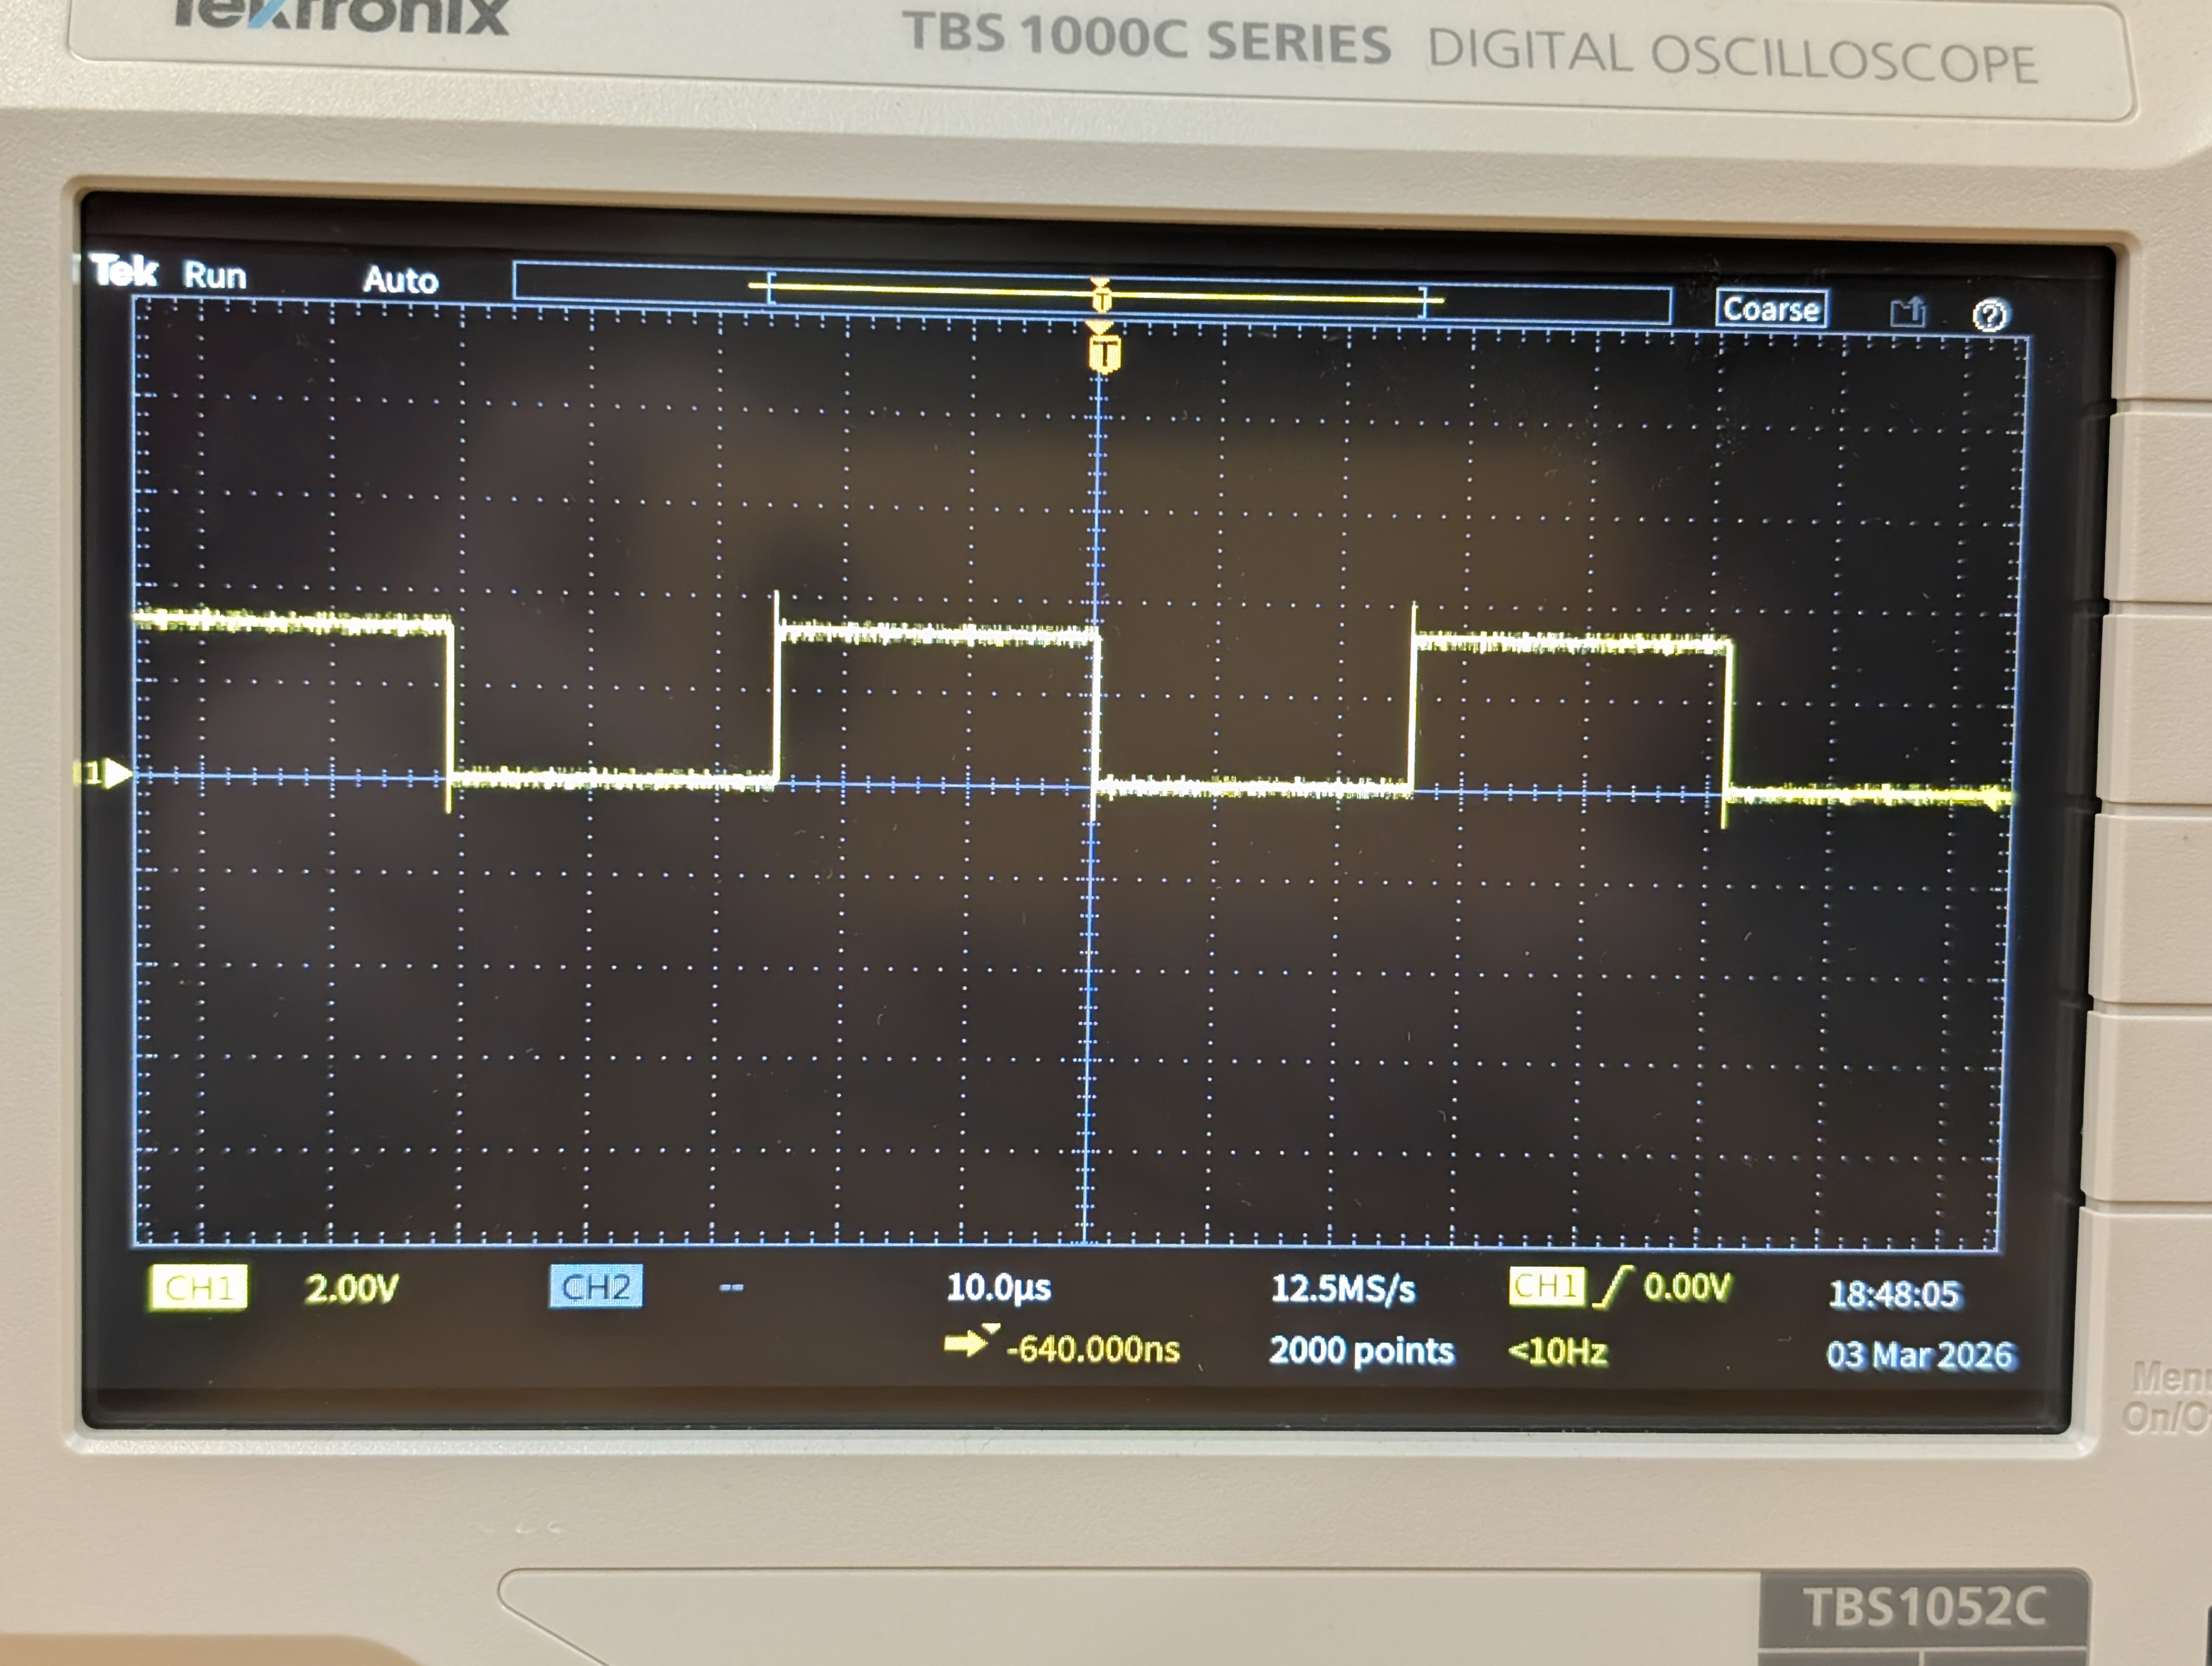
\includegraphics[width=0.45\textwidth]{IMG/Real/PWM_signal.jpg}
    \caption{Oscilloscope capture of the PWM control signal (50\% Duty Cycle)}
    \label{fig:pwm_signal}
\end{figure}

\subsection{Encoder Integration and Signal Conditioning}
The final phase of the assembly involved the integration of the motor encoders. Given that the encoders were powered at 5V, it was necessary to ensure the output signals were compatible with the ESP32's 3.3V logic level. To achieve this, a custom signal conditioning board was realized by soldering \textbf{10k$\Omega$ pull-down resistors} on a prototyping PCB for all 8 encoder channels (A/B phases for 4 motors). This setup, shown in Figure \ref{fig:pulldown_logic}, effectively clamped the input signal to approximately \textbf{3.4V}.

\begin{figure}[H]
    \centering
    \begin{minipage}[b]{0.63\textwidth}
        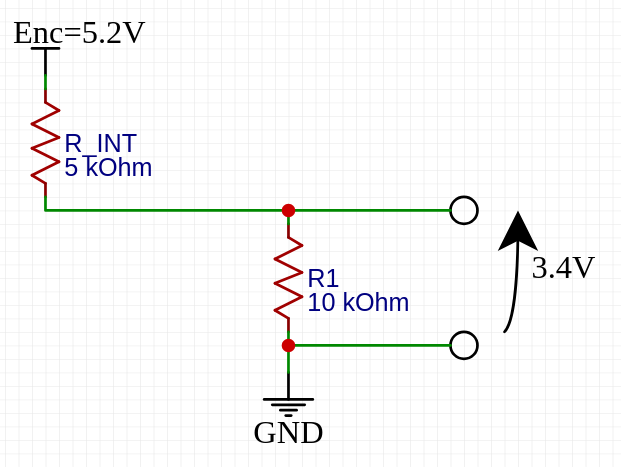
\includegraphics[width=0.6\textwidth]{IMG/Real/pulldown_resistor.png}
        \caption{Pull-down resistor implementation for signal conditioning }
        \label{fig:pulldown_logic}
        \end{minipage}
        \hfill
    \begin{minipage}[b]{0.32\textwidth}
        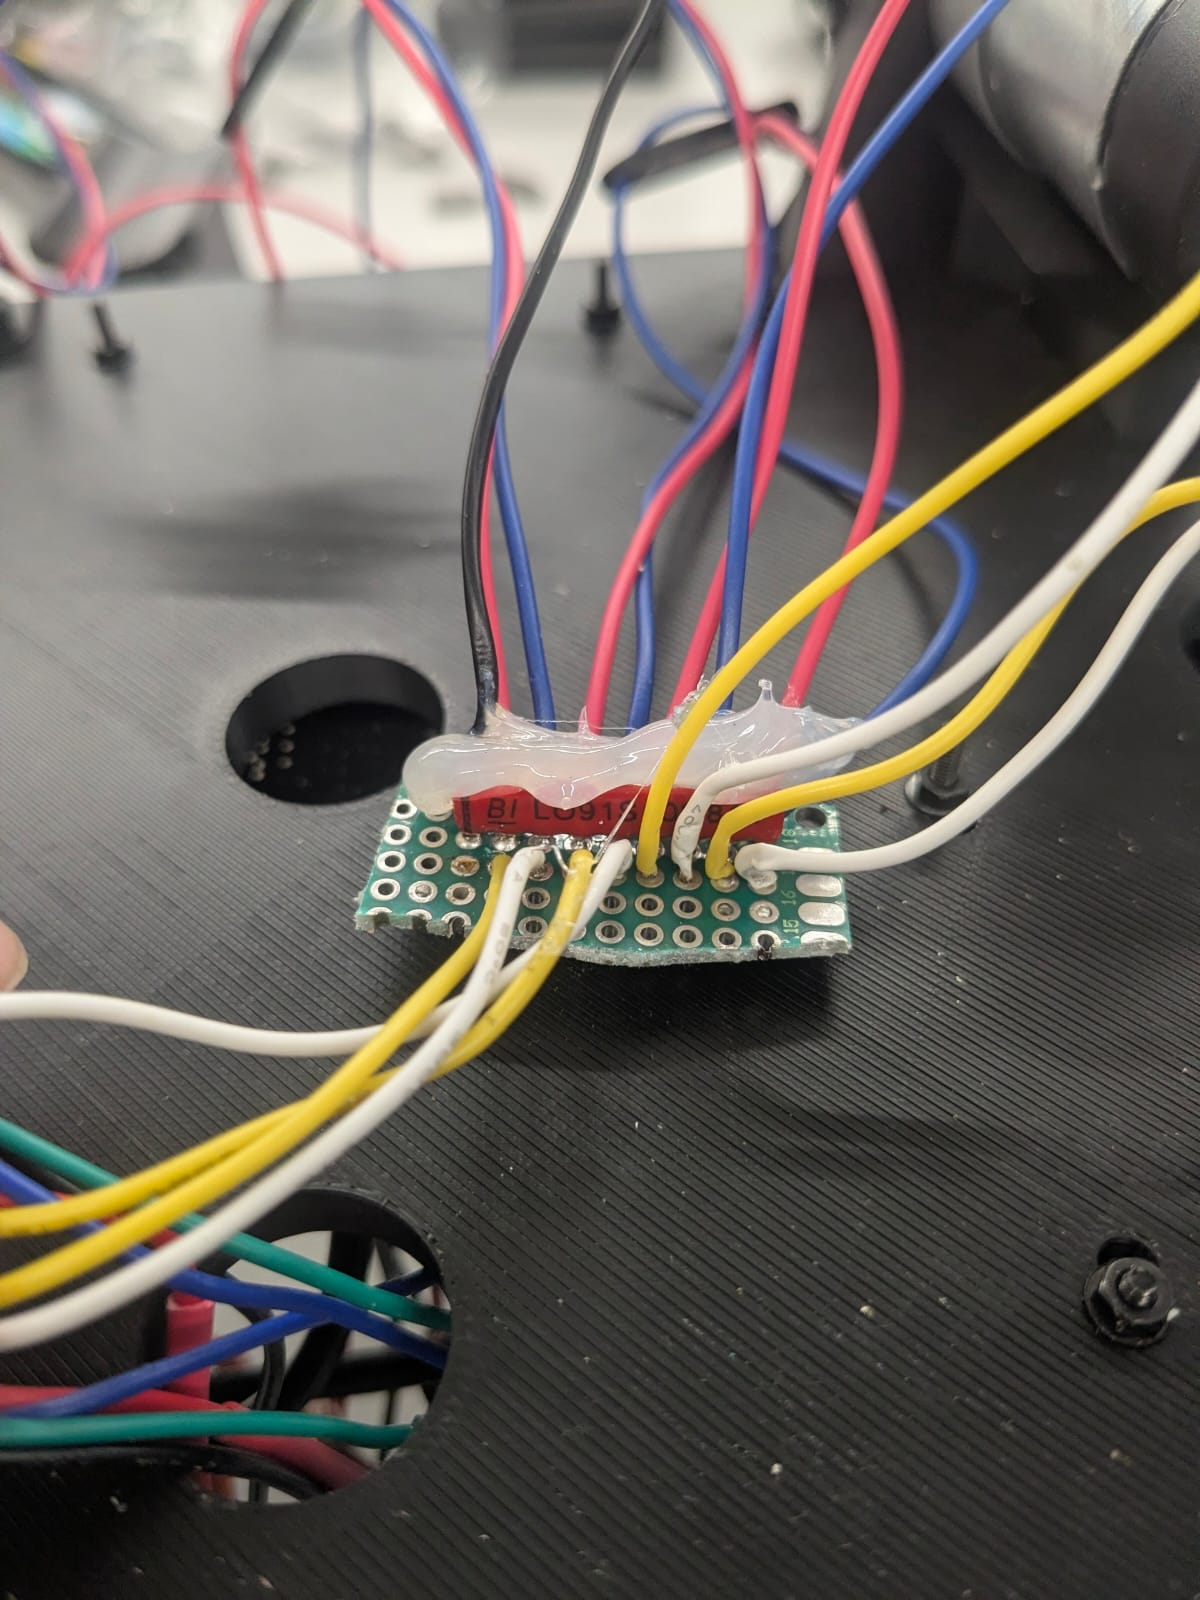
\includegraphics[width=0.6\textwidth]{IMG/Real/pulldown_real.jpeg}
        \caption{Real application of Pull-down resistor}
        \label{fig:pulldown_logic_Real}
        \end{minipage}
    \caption{Solution for Encoder signal}
    \label{fig:Solution for Encoder signal}
\end{figure}

The resulting waveforms were verified via oscilloscope for both forward and backward rotations (Figure \ref{fig:encoder_signals}). The quadrature relationship between the signals remained consistent, providing the high-resolution feedback required for accurate odometry.

\begin{figure}[H]
    \centering
    \begin{minipage}[b]{0.48\textwidth}
        \centering
        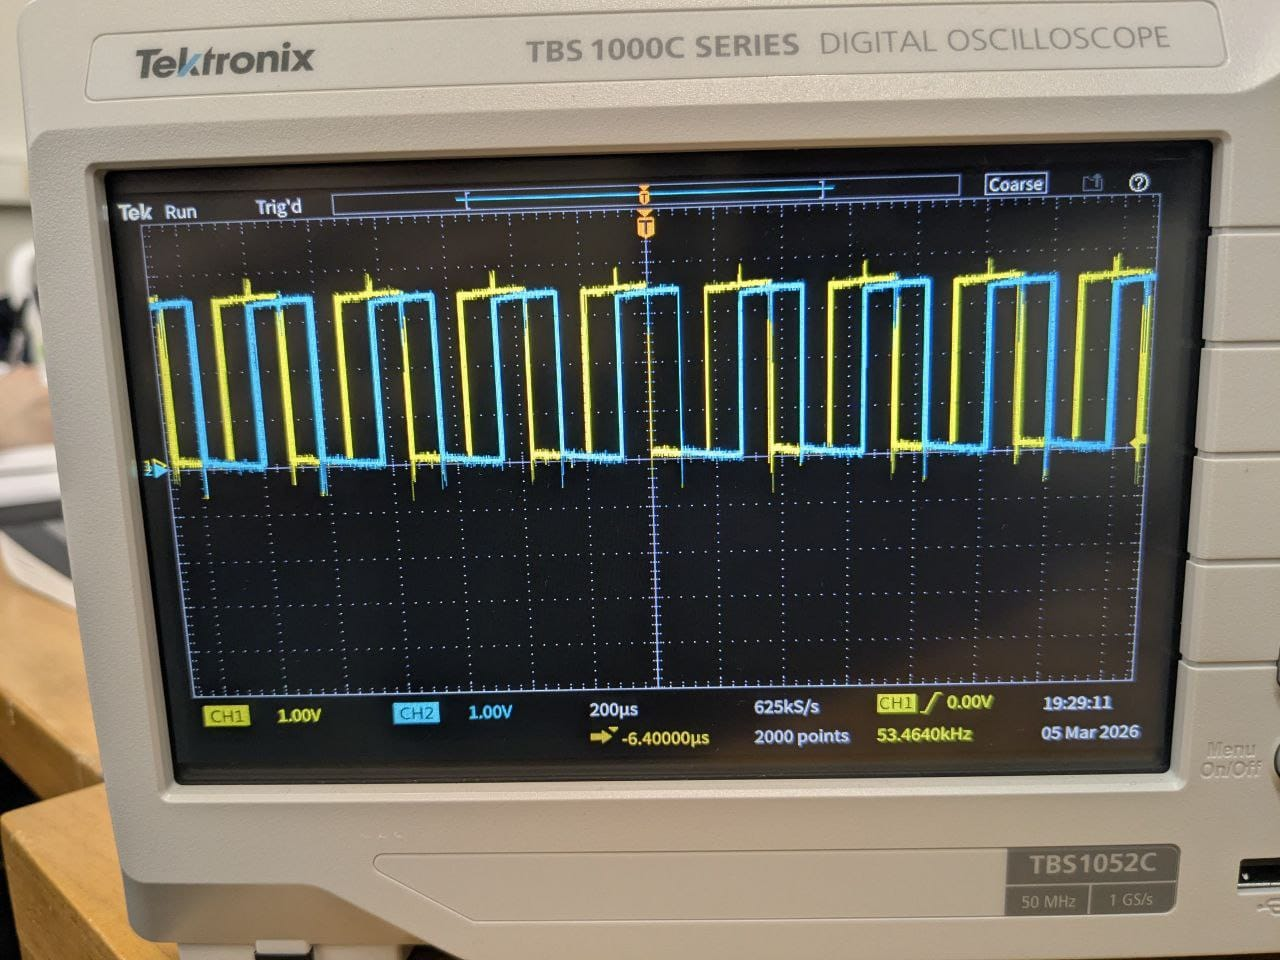
\includegraphics[width=\textwidth]{IMG/Real/encoder_forward.jpeg}
        \caption*{Forward rotation signal}
    \end{minipage}
    \hfill
    \begin{minipage}[b]{0.48\textwidth}
        \centering
        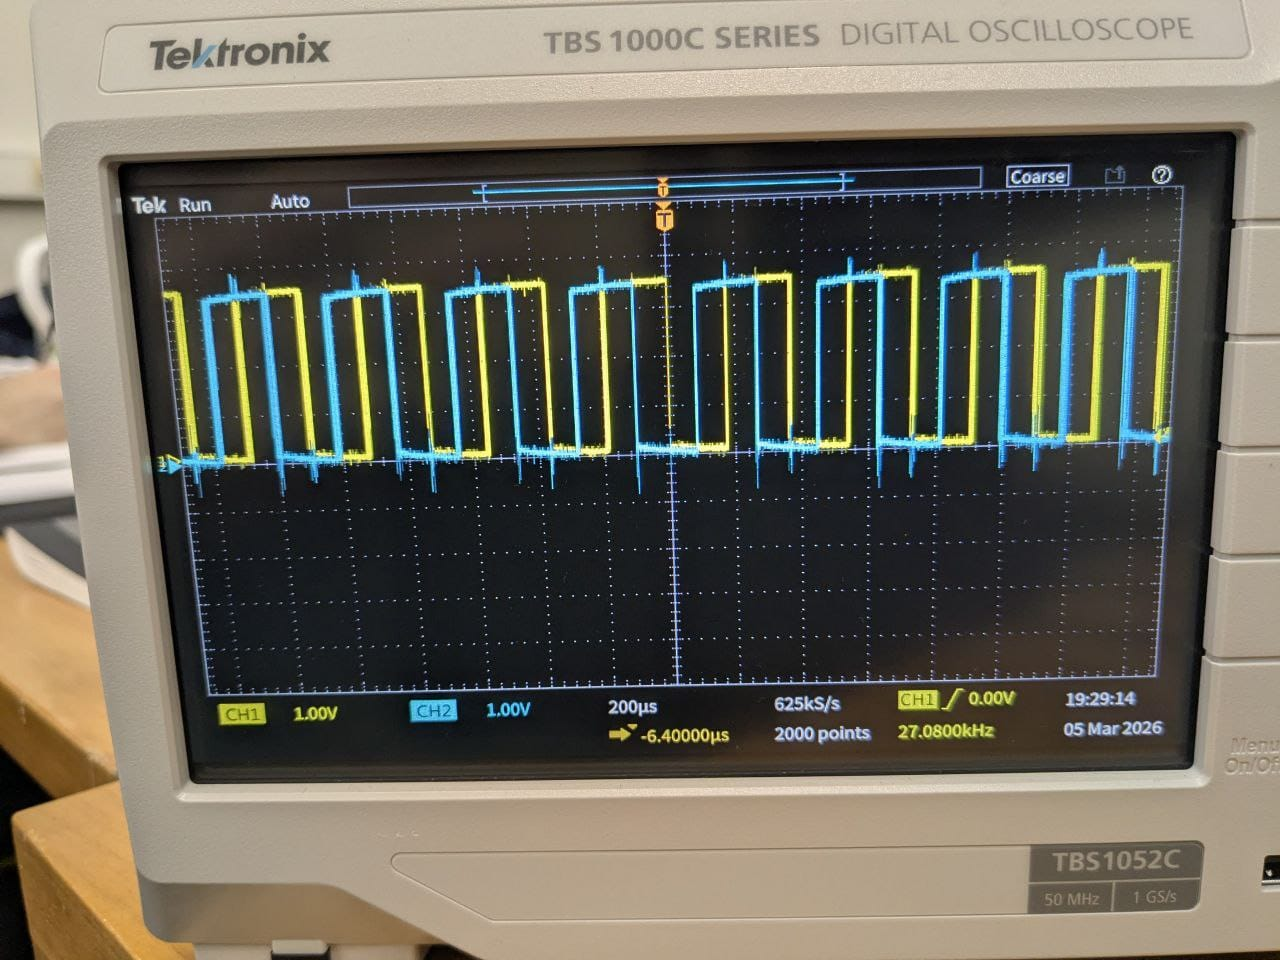
\includegraphics[width=\textwidth]{IMG/Real/encoder_backward.jpeg}
        \caption*{Backward rotation signal}
    \end{minipage}
    \caption{Conditioned encoder signals (approx. 3.4V peak-to-peak)}
    \label{fig:encoder_signals}
\end{figure}

The completion of these hardware validation steps allowed for the commencement of the first dynamic field tests on the integrated platform.

\begin{figure}[H]
    \centering
    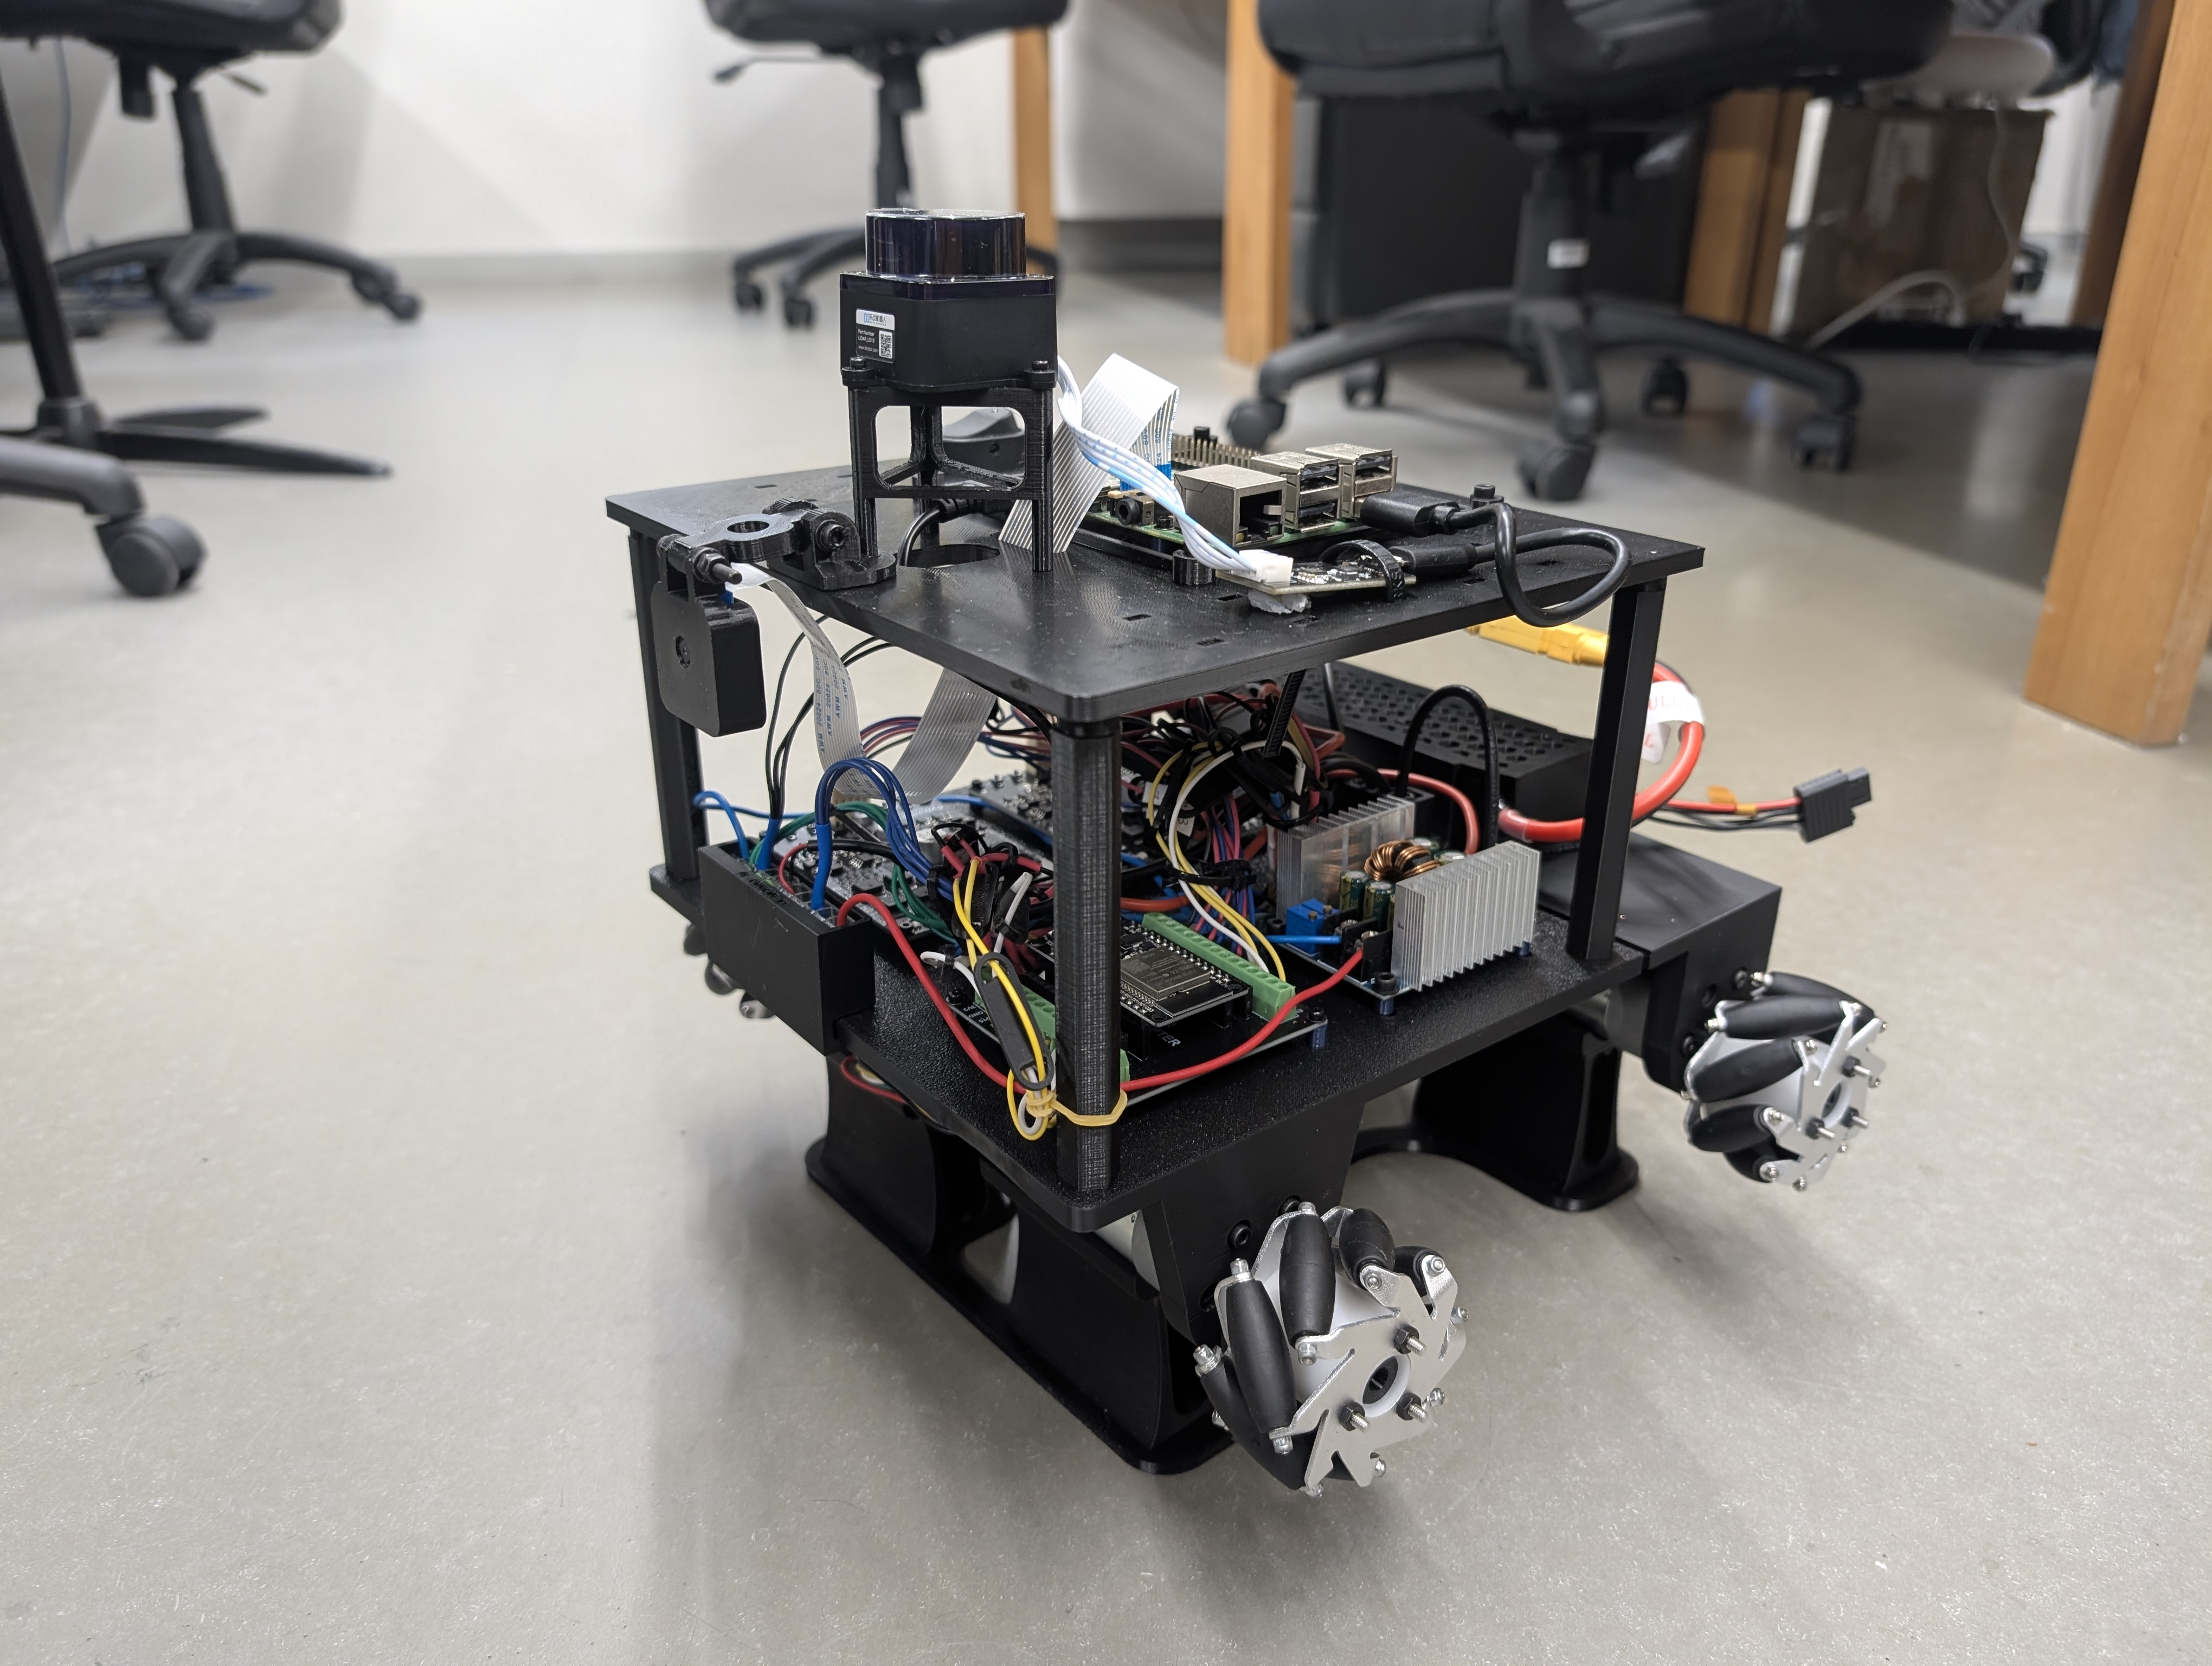
\includegraphics[width=0.7\textwidth]{IMG/Real/Real_omnicar_2.jpg}
    \caption{Fully assembled OMNICAR platform ready for field testing}
    \label{fig:final_robot}
\end{figure}
\chapter{Firmware Development and Experimental Validation}
\label{chap:firmware}

\section{Development Environment: ESP32 and PlatformIO}

The OMNICAR project utilizes the ESP32 microcontroller as the core low-level control unit. Given the necessity to manage high-frequency tasks—such as reading four independent encoders and executing real-time control loops—the development environment played a critical role in ensuring system reliability. While the Arduino IDE is suitable for rapid prototyping, it lacks the advanced features required for complex, multi-file robotic projects. Consequently, the development was migrated to \textbf{PlatformIO}, an open-source ecosystem for IoT development integrated into Visual Studio Code.

The choice of PlatformIO was driven by several technical advantages essential for the OMNICAR's firmware architecture:

\begin{itemize}
    \item \textbf{Modular Project Structure}: Unlike the flat file structure of Arduino, PlatformIO encourages a professional C++ organization. By separating declarations in header files (\texttt{.h}) and logic in implementation files (\texttt{.cpp}), the project achieved better encapsulation and significantly reduced compilation times through incremental builds.
    \item \textbf{Advanced Debugging and Monitoring}: The integrated serial monitor, configured at 115200 baud, allowed for real-time telemetry of motor speeds and PID performance. Furthermore, the environment's support for hardware debugging was pivotal during the initial validation of the encoder reading tasks.
    \item \textbf{Remote Deployment and Diagnostics (OTA)}: Since the OMNICAR is a mobile platform, frequent firmware updates via USB were impractical during dynamic field tests. PlatformIO's native support for \textbf{ArduinoOTA} (Over-The-Air) enabled wireless flashing of the ESP32 over the local network, allowing for immediate iterations. Furthermore, this setup facilitated the analysis of offline floor tests by sharing log files through an integrated \textbf{Web Server} hosted on the ESP32's IP address, eliminating the need for physical access to the robot's internal hardware.
\end{itemize}

\subsection{Configuration: the platformio.ini file}

The \texttt{platformio.ini} file is the core of the project configuration. It allows for precise control over the compilation environment, library versions, and upload methods. Below is the specific setup used for the OMNICAR:

\begin{vscode}{platformio.ini}
[env:esp32dev]
platform = espressif32 @ 6.5.0
board = esp32dev
framework = arduino

; Over-the-Air update configuration
upload_protocol = espota
upload_port = 192.168.31.144  	; IP address ESP32

monitor_speed = 115200 		  	;BaudRate serial monitor
lib_deps = 
    adafruit/Adafruit ADS1X15 @ ^2.5.0
    adafruit/Adafruit BusIO @ ^1.14.1
    bblanchon/ArduinoJson @ ^6.21.3

build_flags = 
    -D CORE_DEBUG_LEVEL=3
    -D _USE_MATH_DEFINES

build_src_filter = +<*> -<PID.cpp>
\end{vscode}

As previously mentioned, the implementation of the \texttt{espota} protocol proved to be fundamental during the experimental phase. It enabled wireless firmware updates while the robot remained positioned on the floor, thereby eliminating the need for constant physical tethering.

\section{Software Architecture and Project Structure}

The firmware is developed using an Object-Oriented Programming (OOP) approach to manage the complexity of the four-wheeled omnidirectional system. The separation of declarations (\texttt{.h}) and implementations (\texttt{.cpp}) is fundamental to ensure modularity (module like motor, encoder, communication, control), allowing for independent testing of hardware components like motors and encoders.

The ESP32 project hierarchy, as organized within the PlatformIO environment, is structured as follows:

\begin{folderbox}{ESP32 Project Directory Structure}
\dirtree{%
.1 OmniCar\_Control/[02]Code/Omnicar/.
.2 .pio/ \DTcomment{Build files and libraries}.
.2 include/ \DTcomment{Header files (.h)}.
.3 connection.h \DTcomment{WiFi and MQTT protocols}.
.3 log.h \DTcomment{Serial and network log}.
.3 motor.h \DTcomment{Control interface (PWM/DIR)}.
.3 CtrlPID.h \DTcomment{PID control class}.
.3 robot.h \DTcomment{Robot class aggregation}.
.3 robot\_config.h \DTcomment{Hardware pins and kinematics}.
.3 encoder.h \DTcomment{Encoder and speed estimation}.
.2 lib/ \DTcomment{External managed libraries}.
.3 Adafruit\_ADS1115.
.3 Adafruit\_BusIO.
.3 ArduinoJson.
.2 src/ \DTcomment{Implementation files (.cpp)}.
.3 main.cpp \DTcomment{Core logic and loops}.
.3 connection.cpp.
.3 motor.cpp.
.3 CtrlPID.cpp.
.3 robot.cpp.
.3 encoder.cpp.
.2 platformio.ini \DTcomment{Build configuration}.
}
\end{folderbox}

\subsection{Role of Main Components}
To ensure a clear distinction between high-level logic and low-level hardware control, the following roles have been assigned to the primary modules:

\begin{itemize}
    \item \textbf{Robot Class (\texttt{Robot.h/cpp})}: 
    Acts as the central hardware abstraction layer and orchestrator for the firmware. It encapsulates the state of the entire platform by aggregating instances of \texttt{Motor} objects and PID controllers. It is responsible for executing the main control loop at a deterministic frequency (e.g., 50Hz, 100Hz, 200Hz), updating the kinematic model, and synchronizing the flow of data between the low-level hardware (actuators/sensors) and the communication layer.

    \item \textbf{Motor \& Encoders}: 
    These low-level modules handle the direct interface with the hardware drivers. The Motor module translates velocity setpoints into PWM signals (using ESP32 peripherals or external drivers like MDD10A) to control the motors. The Encoder module processes signals—capturing ticks via interrupts or dedicated hardware—to compute real-time angular position and velocity for the feedback loop.

    \item \textbf{Connection Handler}: 
    Manages the communication bridge between the embedded controller (ESP32) and the high-level planner (Raspberry Pi/ROS). It implements the protocol stack to parse incoming command packets (e.g., velocity vectors) and serializes telemetry data (encoders, battery status). It supports multiple transport layers, such as high-speed Serial (UART) for real-time control or MQTT/WiFi for remote monitoring and logging.

    \item \textbf{Robot Config (\texttt{robot\_config.h})}: 
    A centralized configuration header that serves as the "single source of truth" for the system. It contains all calibrated hardware constants—such as pin mappings, kinematic dimensions, gear ratios, and PID gains. This decoupling prevents hard-coded values in the logic files, facilitating easy tuning and adaptation to different hardware revisions without modifying the core source code.
    
\end{itemize}

\section{Hardware Abstraction: robot\_config.h}

The \texttt{robot\_config.h} file acts as a centralized configuration hub. It contains critical hardware parameters such as:
\begin{itemize}
    \item \textbf{Pin Mapping}: GPIO assignments for PWM and DIR signals for the four MDD10A drivers.
    \item \textbf{Kinematics}: Wheel radius, gear ratios, and robot geometry ($L$ and $l$ distances).
    \item \textbf{Encoder Resolution}: Definition of the counts per revolution (CPR) to ensure accurate odometry.
\end{itemize}

The \texttt{robot\_config.h} file acts as a centralized configuration hub, ensuring decoupling between hardware parameters and control logic. It contains critical system constants such as:
\begin{itemize}
    \item \textbf{Pin Mapping}: GPIO assignments for the PWM and DIR (direction) peripherals and digital inputs for the encoder signals.
    \item \textbf{Kinematics}: Geometric definitions for the omnidirectional model, including wheel radius ($r = 0.06$ m), gear ratio ($N = 18.75$), and chassis half-dimensions ($L_x = 0.185$ m, $L_y = 0.220$ m).
    \item \textbf{Encoder Resolution}: Definition of the counts per revolution ($CPR = 64$) used to convert raw ticks into angular velocity.
    \item \textbf{PID Control Tuning}: Specifies the PI controller gains derived via \textit{Internal Model Control} (IMC). The parameters are calculated based on an identified first-order plant model of the motors 
\end{itemize}


\section{Experimental Procedures and Main Loop}

The firmware's operational core is encapsulated within the \texttt{main.cpp} file, which manages the real-time execution loop for the motion control algorithms.

\subsection{System Initialization and Setup}
The \texttt{setup()} function defines a common initialization phase for all experimental procedures. This routine configures the hardware peripherals and communication protocols required for robot operation. Include the initialization of the serial interface at 115,200 baud for telemetry, the configuration of the \texttt{Robot} object, and the setup of the Over-The-Air (OTA) update system.

The \texttt{robot.init()} method assigns the GPIO pins for the MDD10A motor drivers and read the encoder channels. A serial channel protocol is initialized to exchange data between the ESP32 and the Raspberry Pi 5.

\begin{vscode}{main.cpp/setup}
void setup() {
  // Inizializza la seriale per il monitoraggio
  Serial.begin(115200);
  serial_channels.init(processSerialPacket, serialWrite);
  // Configura il pulsante BOOT (GPIO 0)
  pinMode(0, INPUT_PULLUP);

  // --- WIFI, OTA, WEB SERVER SETUP ---
  setupWiFi();
  setupOTA();
  // setupWebServer(); //Web Server usato per scaricare i file di log durante le prove offline

  Serial.println("--- OMNICAR MOTOR TEST START ---");
  Serial.flush();
  // Inizializza il robot passando la funzione di callback per la seriale
  robot.init(serialWriteChannel);
  Serial.println("Robot initialized.");
  
  // Reset signal
  serialWriteChannel('r', 0);
  // Initialization
  current_micros = micros();
  previous_micros = current_micros;
  last_motor_update_millis = millis();
}
\end{vscode}

\subsection{Encoder Validation and Tick Counting}
The initial experimental phase consisted of a manual rotation test performed on a selected motor to calibrate and validate the encoder resolution. Although the hardware specifications indicated a nominal resolution of 1200 pulses per revolution (ppr), this empirical verification was essential to ensure that the software parameters defined in \texttt{robot\_config.h} accurately reflected the physical behavior of the system. This procedure eliminated potential discrepancies between the theoretical datasheet and the real-time pulse counting logic, providing a reliable foundation for the first-order velocity control loop.

\begin{vscode}{main.cpp/loop\_manuale}
void loop() {
  uint32_t dt = 0; // Variabile delta time per robot.update
  int idx_mot = 0;
  Serial.println("   TEST MANUALE ENCODER (Ruota a mano)/\n Inserisci indice motore (0-3) per iniziare.");

  while (Serial.available() == 0) {
    delay(10);
  }

  idx_mot = Serial.parseInt();
  // Pulisci il buffer seriale (rimuovi newline)
  while (Serial.available()) { Serial.read(); }

  if (idx_mot >= 0 && idx_mot < kNumMot) {
    Serial.printf("--> MONITORAGGIO MOTORE %d ATTIVO\n", idx_mot);
    Serial.println("    Ruota la ruota manualmente.");

    robot.setMotorPWM(idx_mot, 0);

    // Loop finché non si riceve input seriale
    while (Serial.available() == 0) {
      robot.update(dt);
      Serial.printf("MOT[%d] | Ticks: %d | Odo: %d\n", idx_mot, robot.enc[idx_mot].tick, robot.enc[idx_mot].odo);
    }
  } else {
    Serial.printf("Indice %d non valido! Inserire 0, 1, 2 o 3.\n", idx_mot);
  }
}
\end{vscode}

\subsection{Open-Loop Response and First-Order Approximation}
Individual motors were driven at specific PWM duty cycles to validate the assumption of a \textbf{first-order system} model. To derive this model, we consider the electromechanical equations of a DC motor in the Laplace domain ($s$-domain):

\begin{equation}
\begin{cases}
    U(s) = (R + sL)I(s) + K\Omega(s) \\
    sJ\Omega(s) = KI(s) - B\Omega(s) - T_q
\end{cases}
\begin{cases}
    U(s) = (R + sL)I(s) + K\Omega(s) \\
    KI(s) = (sJ + B)\Omega(s) + T_q
\end{cases}
\end{equation}

where $U(s)$ is the input voltage, $I(s)$ the armature current, $\Omega(s)$ the angular velocity, and $T_q$ represents the load torque. 

\subsubsection{Linearization and Order Reduction}
It is important to note that a linear transfer function $\frac{\Omega(s)}{U(s)}$ cannot be directly deduced from the equations above because the term $T_q$ renders the expression affine rather than linear. To achieve a linear representation, we assume $T_q = 0$, with the intention of compensating for this physical nonlinearity later. Under this assumption, the system can be rearranged as:

\begin{equation}
    \frac{\Omega(s)}{U(s)} = \frac{K}{(R + sL)(sJ + B)}
\end{equation}

resulting in a second-order system. In this scenario, the electrical pole ($s = -R/L$) is typically much faster (located much further left in the complex plane) than the mechanical pole ($s = -B/J$). Consequently, the high-frequency electrical dynamics can be neglected, leading to the final first-order approximation:

\begin{equation}
    G(s) = \frac{\Omega(s)}{U(s)} \approx \frac{K_{gain}}{sJ + B} = \frac{A}{\tau s + 1}
\end{equation}


\subsection{Double Step Test for PID Tuning}
As specified in the \texttt{robot\_config.h} file, the nominal control frequency was established at 50 Hz, although the system performance at higher frequencies was also evaluated in specific test cases. Prior to the formal identification of the system parameters, a preliminary test was conducted on a single motor under no-load conditions. The resulting angular velocity $\omega(t)$, measured in rad/s, is illustrated in Figure \ref{fig:First Test PWM in 50Hz}.

The experimental procedure involved a double-step input: the first step applied a PWM duty cycle of 2047 (representing approximately half of the maximum available thrust), while the second step reached the full resolution of 4095. The steady-state angular velocities observed during these tests align closely with idealized theoretical values, peaking at approximately $60$ rad/s. 

Notably, the open-loop response under no-load conditions show marginal noise and reaches the target velocity with high precision. The purely asymptotic profile of the curve provides visual confirmation that the electrical dynamics—associated with the second pole of the system—are effectively negligible compared to the mechanical time constant. This empirical evidence further justifies the adoption of a first-order approximation for the velocity control loop.

\begin{figure}[H]
    \centering
    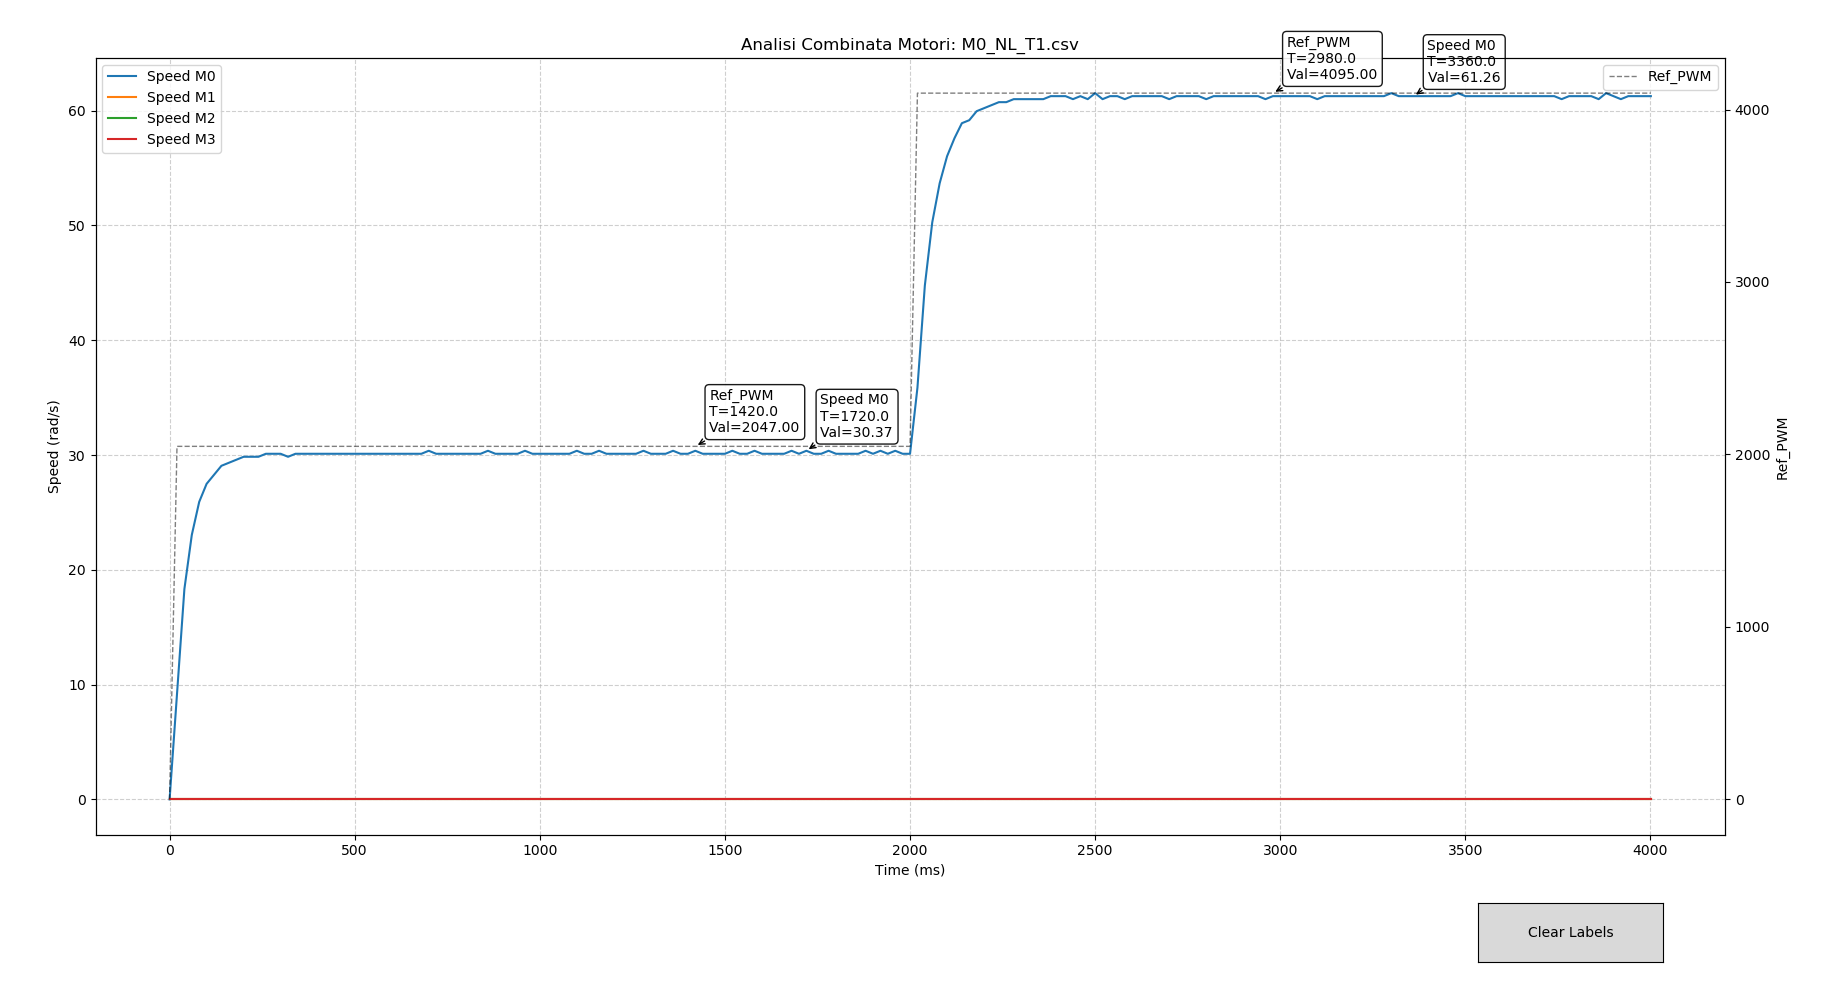
\includegraphics[width=1\textwidth]{IMG/PID/M0_Primo_TEST_PWM.png}
    \caption{First Test PWM in 50Hz}
    \label{fig:First Test PWM in 50Hz}
\end{figure}

A double-step input was applied to all four motors simultaneously during a test with load (robot on the floor). By measuring the steady-state speed we can calculating the gain and the time constant ($\tau$).

As illustrated in Figures \ref{fig:MA_NL_T2_50hz}, \ref{fig:MA_NL_T2_50hz_Mot2}, and \ref{fig:MA_NL_T2_50hz_Separato}, specific safety PWM thresholds were established for the step response tests: a first step at 750 and a second at 1500. These duty cycle values correspond approximately to angular velocities of 10 rad/s and 20 rad/s, respectively.

In this phase, isolating the individual motor responses was fundamental to detecting any potential mechanical or electrical anomalies. The experimental data confirms that all motors exhibit consistent behavior, characterized by a decoupled and uniform response across the assembly.

Based on the analysis of the collected data, the following system parameters were identified. First, the PWM signals were converted into their equivalent voltage values using the following relation:

\begin{equation}
    V_{pwm} = \frac{PWM_{ref}}{PWM_{max}} \cdot V_{battery}
\end{equation}

Given a maximum resolution $PWM_{max} = 4095$ and a measured battery voltage $V_{battery} = 11.9$ V, we obtain:

\begin{equation}
    V_{pwm,750} \approx 2.18 \text{ V}, \quad V_{pwm,1500} \approx 4.36 \text{ V}
\end{equation}

The steady-state gain $K$ was then calculated as the ratio between the variation in angular velocity and the variation in input voltage:

\begin{equation}
    K = \frac{\Delta \omega}{\Delta V_{in}} = \frac{\omega_2 - \omega_1}{V_{pwm,1500} - V_{pwm,750}} = 5.04
\end{equation}

To determine the time constant $\tau$, we identified the angular velocity value corresponding to $63.2\%$ of the transient transition between the first and second step:

\begin{equation}
    \omega_{\tau} = \omega_1 + 0.632 \cdot (\omega_2 - \omega_1) = 16.9 \text{ rad/s}
\end{equation}

By locating $\omega_{\tau}$ on the experimental temporal plot, the resulting time constant was estimated to be approximately $\tau \approx 90$ ms.

% --- Open Loop Motor Analysis (MA) Tests ---
\begin{figure}[H]
    \centering
    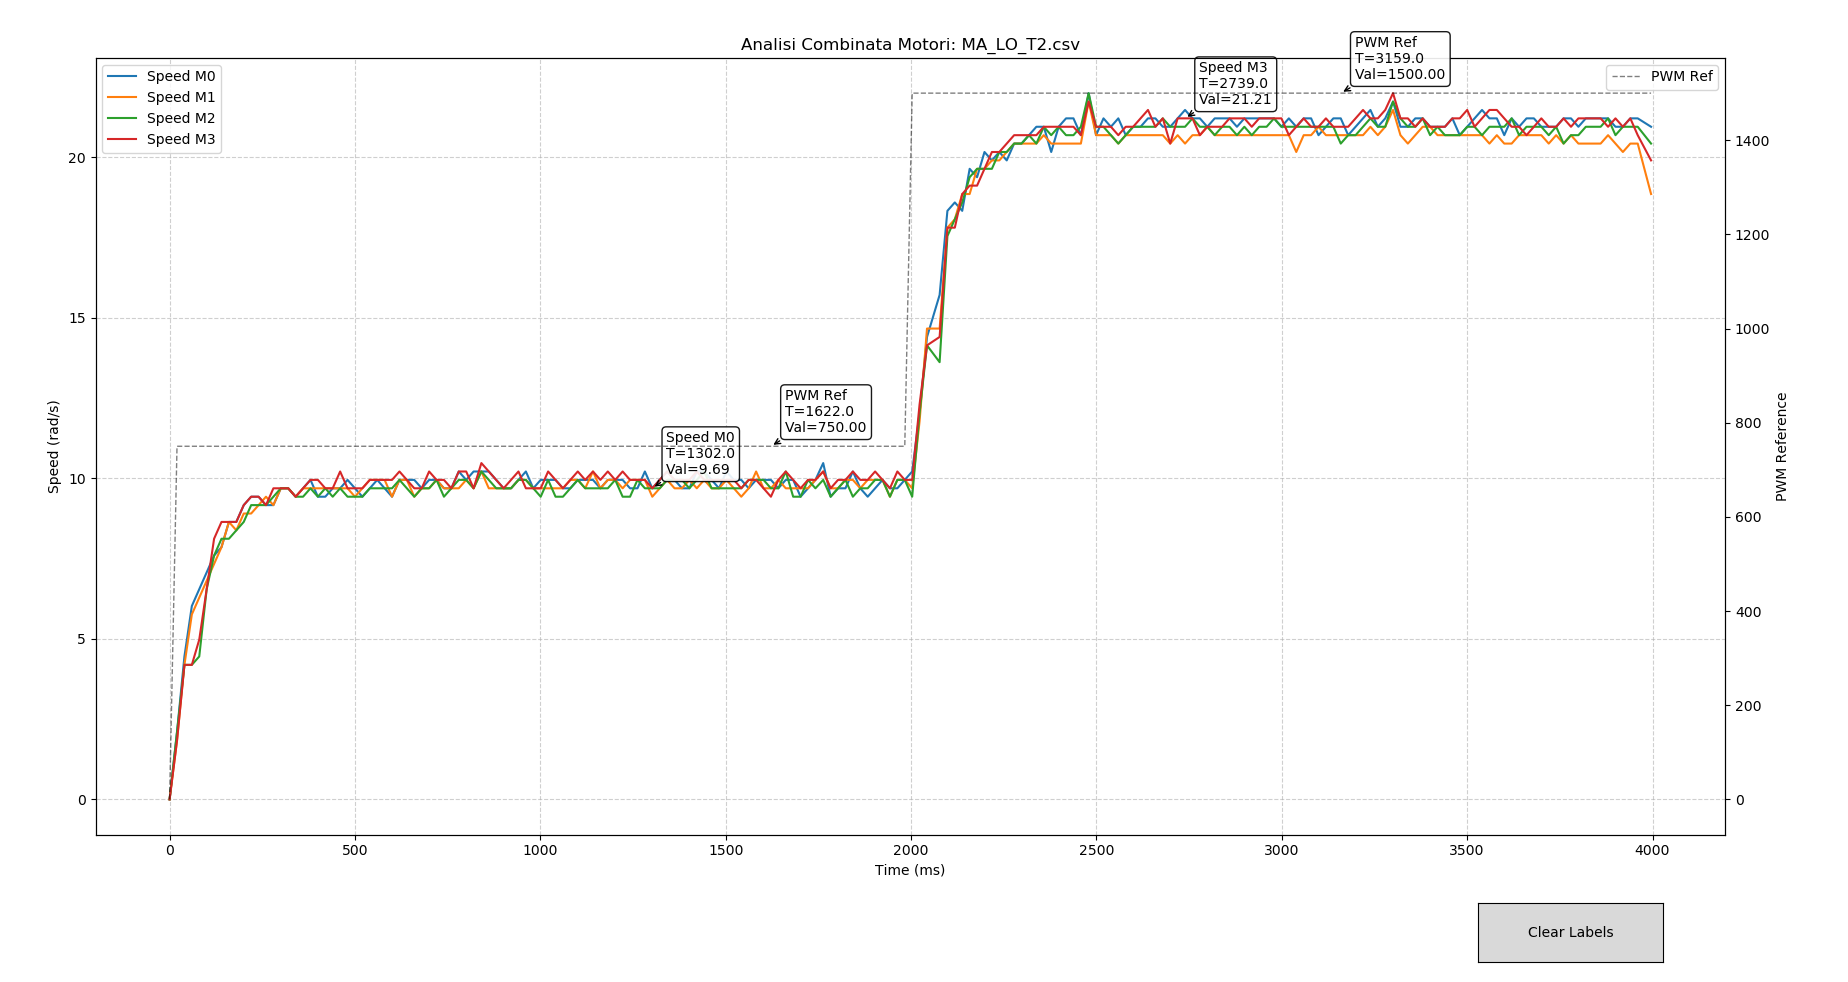
\includegraphics[width=1\textwidth]{IMG/PID/MA_NL_T2_50hz.png}
    \caption{Open-loop no-load test (MA\_NL) at a sampling frequency of 50 Hz}
    \label{fig:MA_NL_T2_50hz}
\end{figure}

\begin{figure}[H]
    \centering
    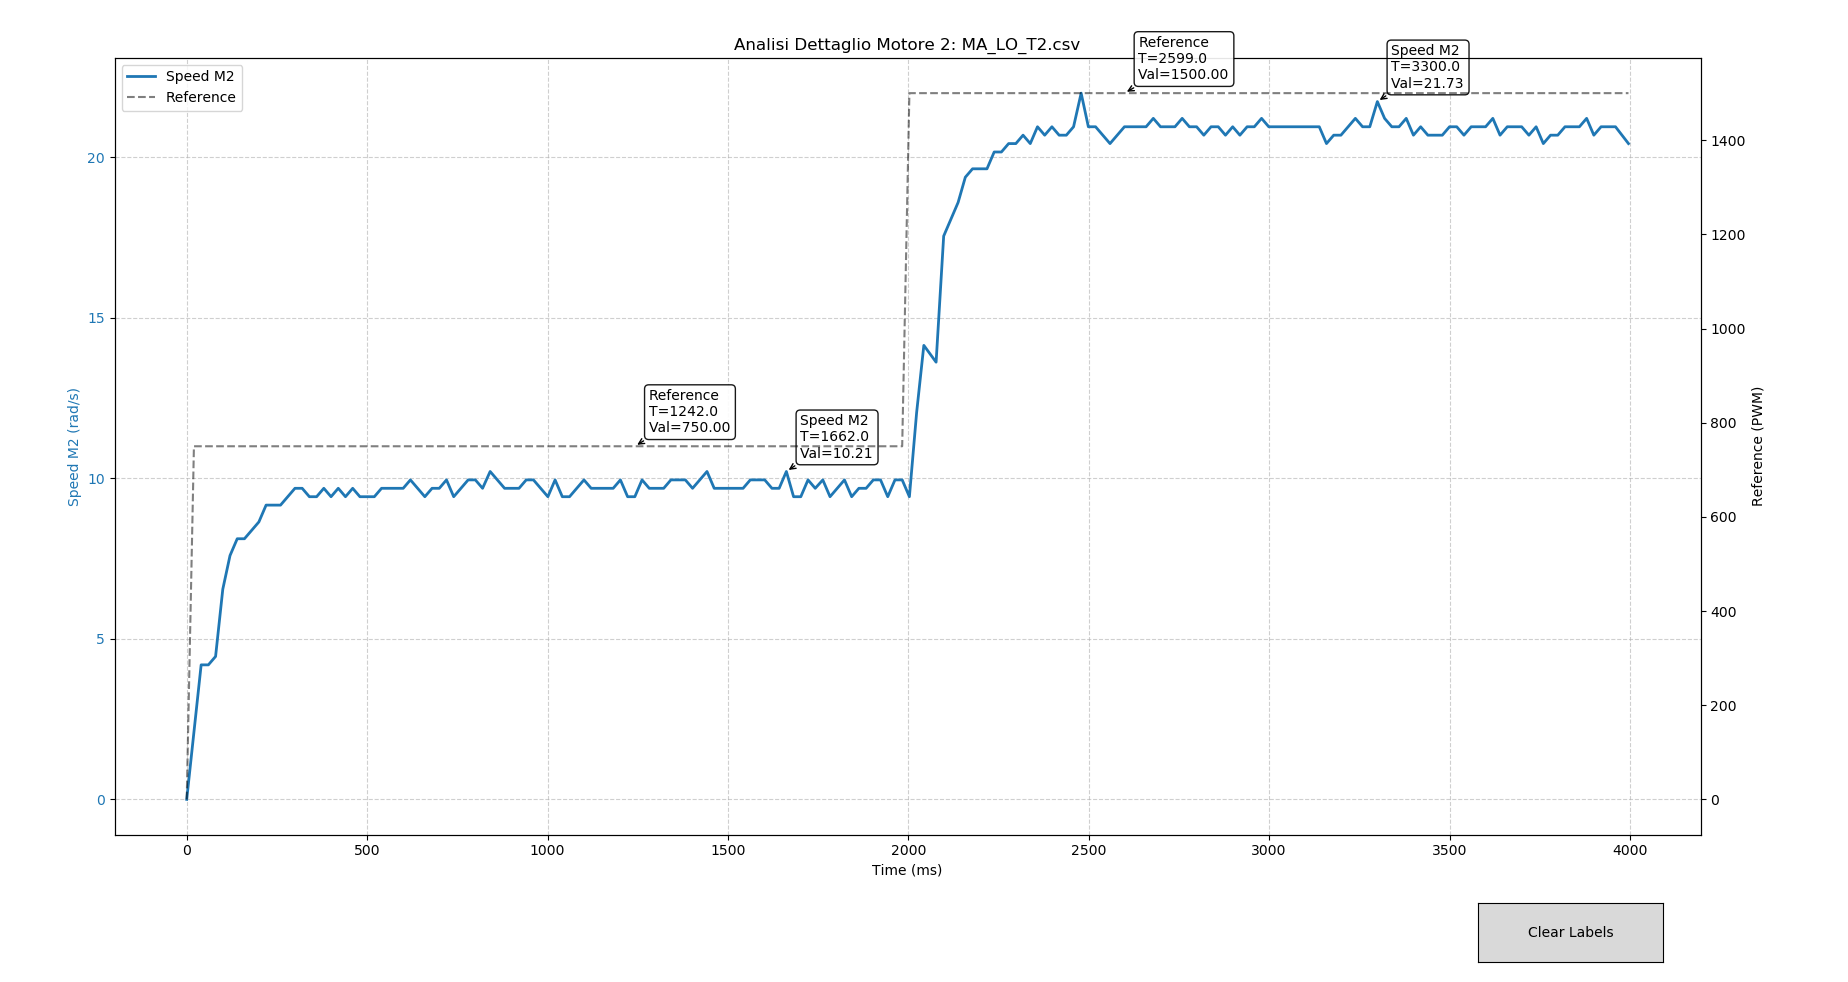
\includegraphics[width=1\textwidth]{IMG/PID/MA_NL_T2_50hz_Mot2.png}
    \caption{Open-loop velocity profile for Motor 2 at 50 Hz sampling rate}
    \label{fig:MA_NL_T2_50hz_Mot2}
\end{figure}

\begin{figure}[H]
    \centering
    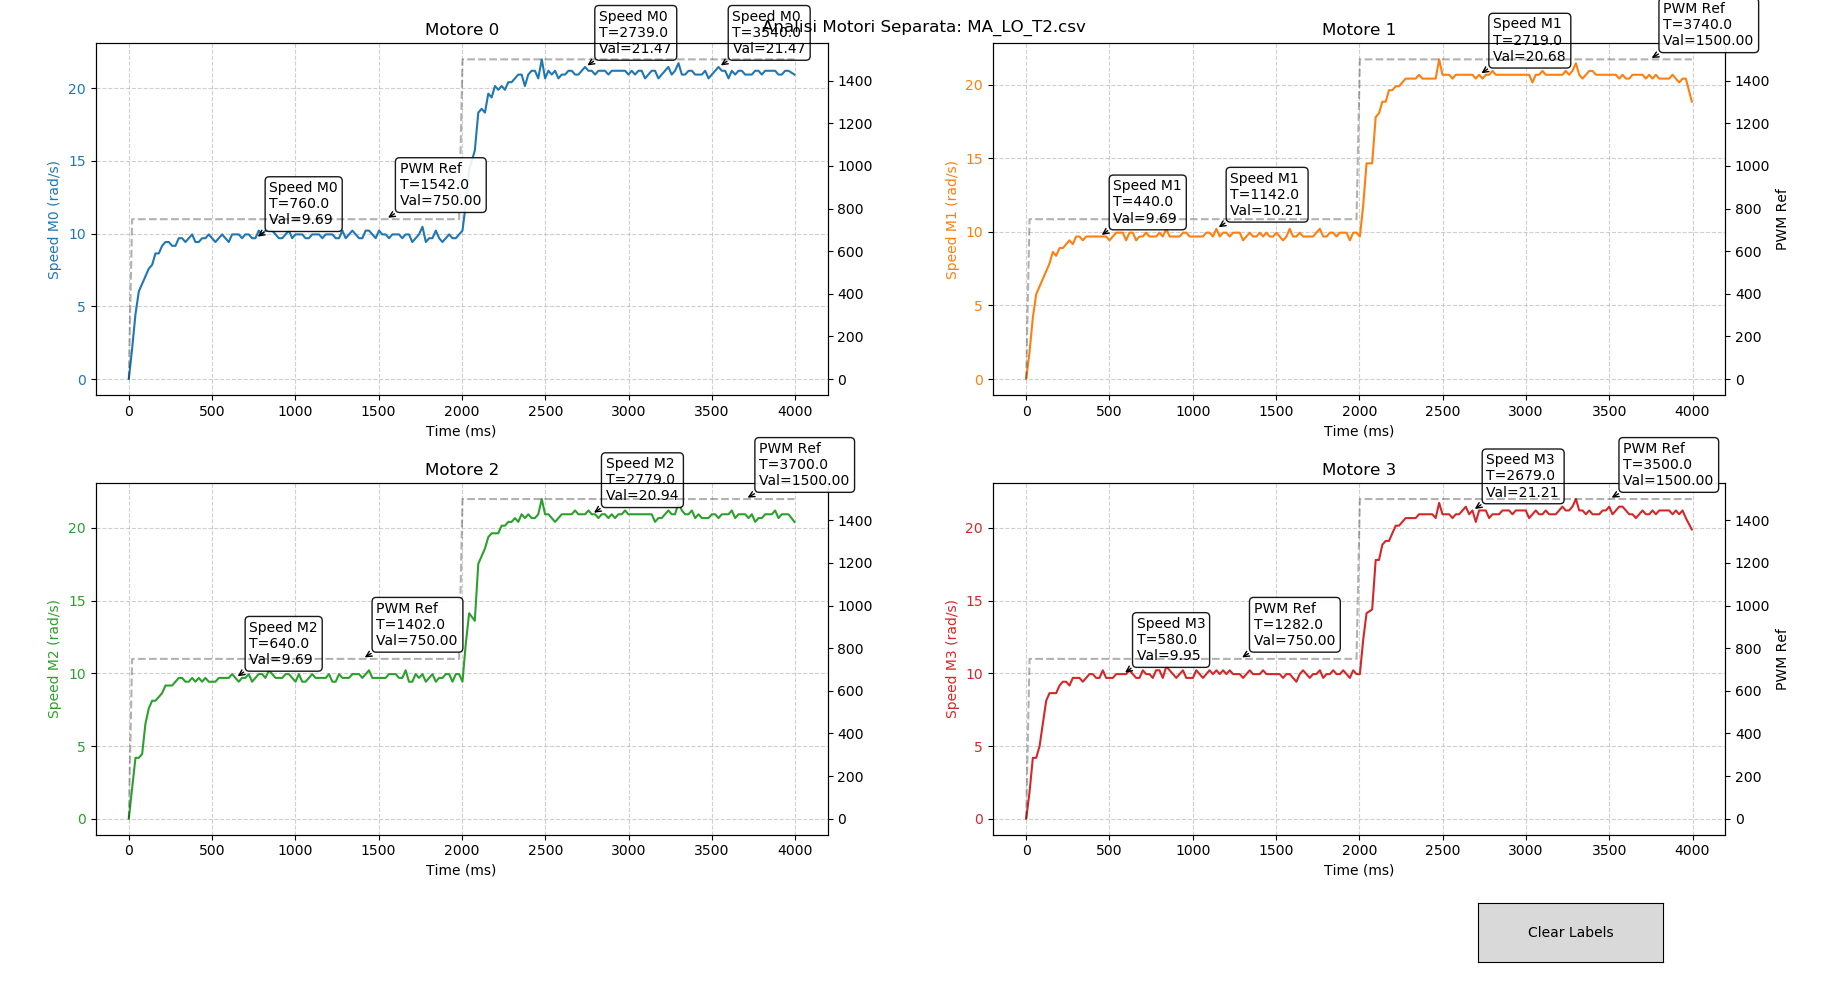
\includegraphics[width=1\textwidth]{IMG/PID/MA_NL_T2_50hz_Separato.png}
    \caption{Detailed view of the open-loop response at 50 Hz for system identification}
    \label{fig:MA_NL_T2_50hz_Separato}
\end{figure}

How show in Figure \ref{fig:MA_NL_T5_100hz}. Experimental analysis demonstrated that increasing the control frequency beyond 50 Hz significantly degrades the Signal-to-Noise Ratio (SNR) in velocity estimation. This phenomenon is primarily attributable to the reduction in numerical resolution—specifically, the quantization error of encoder ticks within shorter sampling periods—and temporal jitter affecting the \texttt{kMotCtrlTimeUs} parameter. 

At higher frequencies, interrupt management on the ESP32 introduces variable latencies that lead to asynchronous tick accumulation, resulting in periodic noise spikes. To ensure the stability of the control algorithms and prevent the amplification of these disturbances through derivative terms, the low-level control loop was maintained at 50 Hz. This configuration provides the optimal compromise between temporal determinism and signal resolution.

\par Subsequent phases of the project will involve use of a dedicated communication link with the Raspberry Pi. In this setup, the raw encoder signals will be transmitted directly and evaluated without the onboard conversion to radians. This approach is designed to assess the signal integrity and the effectiveness of processing when operating at sampling frequencies exceeding 50 Hz.

\begin{figure}[H]
    \centering
    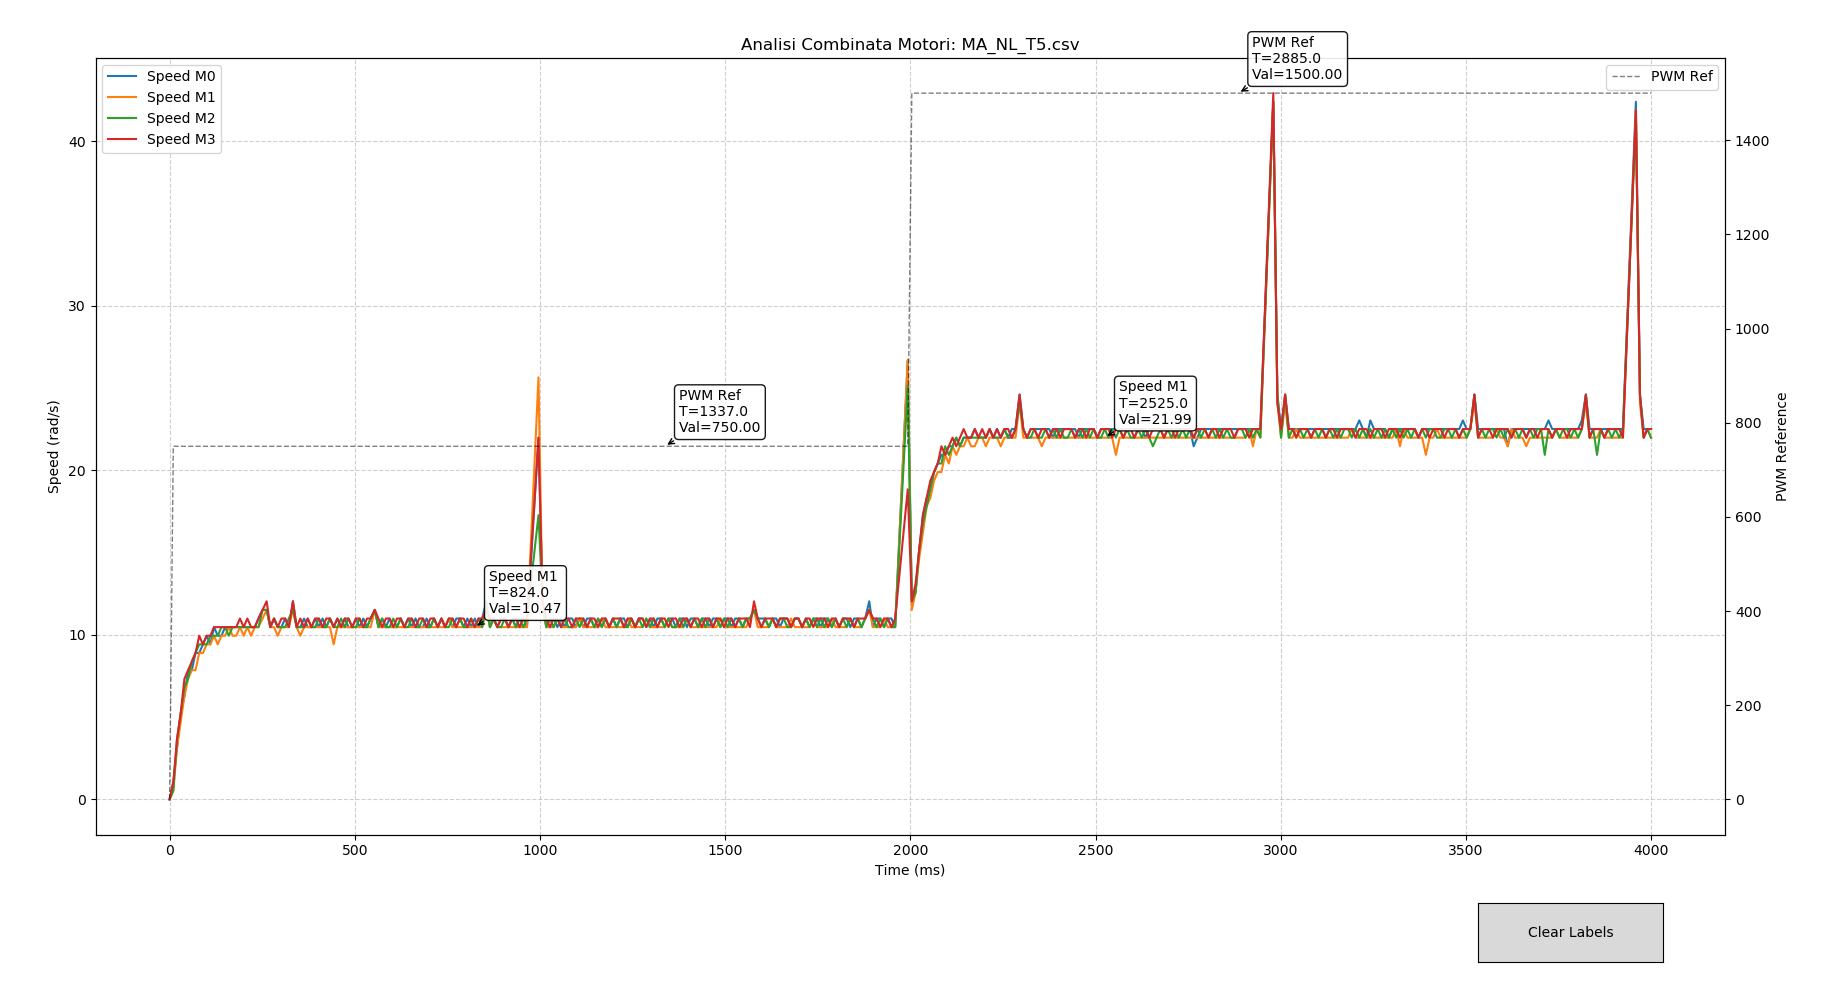
\includegraphics[width=1\textwidth]{IMG/PID/MA_NL_T5_100hz.png}
    \caption{Open-loop test results at 100 Hz showing the initial linear noise increase}
    \label{fig:MA_NL_T5_100hz}
\end{figure}

\begin{vscode}{main.cpp/loop\_tuning}
void loop() {
  ArduinoOTA.handle();
  server.handleClient();  
  handleOfflineTest(); // Controlla pressione tasto

  // Gestione Countdown 5 secondi dopo press BOOT
  if (is_boot_test_pending) {
    if (millis() - boot_test_start_millis > 5000) {
      is_boot_test_pending = false;
      
      // AVVIO TEST E LOG
      logFile = SPIFFS.open("/log.csv", "w");
      if (logFile) {
        tuner.setOutput(&logFile);
        //start(maschera motori attivi, pwm_max, preheat time, step1_time, step2_time)
        tuner.start(0b1111, 1500, 0, 2000, 2000); 
      }
    }
  }

  // Se il tuner è attivo, esegui il suo ciclo di update (non bloccante)
  if (tuner.isRunning()) {
    // Controllo ABORTO: Se premi 'x'
    // (Solo se connesso via seriale)
    if (Serial.available() > 0) {
      char c = Serial.peek(); // Guarda il carattere senza rimuoverlo subito
      if (c == 'x' || c == 'X') {
        Serial.read(); // Rimuovi dal buffer
        tuner.stop();
        return; // Ricomincia il loop
      }
    }
    tuner.update();
  }
  // Chiusura del file log
  else if (logFile) {
    logFile.close();
    tuner.setOutput(&Serial); 
    Serial.println("\n--- LOG SALVATO SU SPIFFS ---");
    Serial.println("Usa il comando 'r' per scaricare i dati.");
  }
  // Altrimenti attendi comandi seriali
  else {
    handleSerialInput();
  }
}
\end{vscode}


\subsection{Closed-Loop}
The transition from open-loop duty cycle commands to a regulated velocity setpoint was achieved through a Proportional-Integral (PI) controller. Since the plant is modeled as a stable first-order system with no zeros, a PI architecture is sufficient to ensure a null steady-state error for step references $R(s) = \frac{1}{s}$.

\subsubsection{Controller Design and Pole-Zero Cancellation}
\begin{figure}[H]
    \centering
    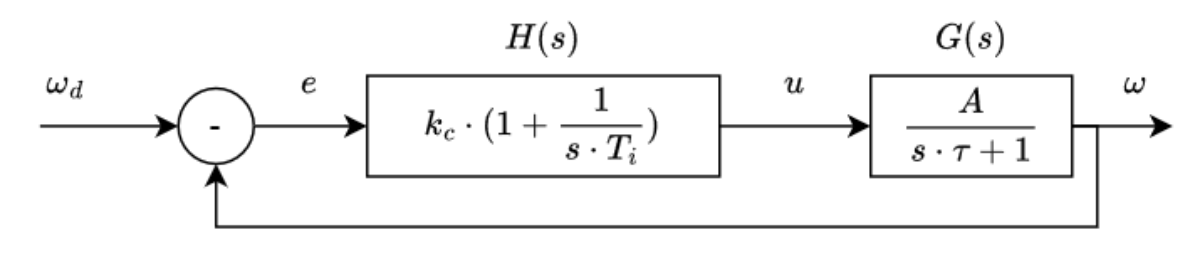
\includegraphics[width=1\textwidth]{IMG/PID/PI_Arch.png}
    \caption{Closed-Loop system - Block diagram}
    \label{fig:PI_Arch}
\end{figure}
Consider the controlling architecture presented in Figure : \ref{}
The controller $H(s)$ is defined by the following transfer function:
\begin{equation}
    H(s) = k_c \left( 1 + \frac{1}{T_i s} \right) = k_c \frac{T_i s + 1}{T_i s}
\end{equation}
where $k_c$ represents the proportional gain and $T_i$ the integral time constant. To simplify the closed-loop dynamics, the design choice $T_i = \tau$ was adopted. This allows the controller's zero to cancel the plant's pole, resulting in the open-loop transfer function:
\begin{equation}
    G(s)H(s) = k_c \frac{A}{\tau s + 1} \cdot \frac{\tau s + 1}{\tau s} = \frac{k_c A}{\tau s}
\end{equation}
The resulting closed-loop transfer function remains a first-order system with unity gain ($A_{cl} = 1$):
\begin{equation}
    T(s) = \frac{G(s)H(s)}{1 + G(s)H(s)} = \frac{1}{\tau_{cl} s + 1}, \quad \text{with } \tau_{cl} = \frac{\tau}{k_c A}
\end{equation}

\subsubsection{Feedforward Compensation and Real-world Constraints}
\begin{figure}[H]
    \centering
    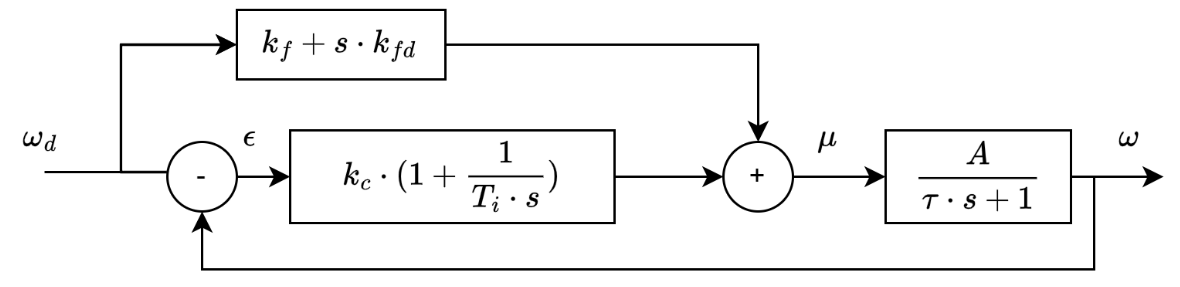
\includegraphics[width=1\textwidth]{IMG/PID/PI_FF_Arch.png}
    \caption{Closed-loop control architecture with feedforward - Block diagram}
    \label{fig:PI_FF_Arch}
\end{figure}
Consider the controlling architecture presented in Figure  \ref{fig:PI_FF_Arch}
To enhance the system's reactivity beyond the feedback loop's limits, a Feedforward (FF) action $F(s)$ was considered. Ideally, the FF controller should invert the plant dynamics ($F(s) = 1/G(s)$) to achieve $F(s)G(s) = 1$. However, a full inversion $\frac{\tau s + 1}{A}$ would be non-proper, requiring a derivative term $k_d$ that is physically unrealizable and highly sensitive to noise. 
Therefore, a simplified feedforward gain was implemented as the inverse of the steady-state gain:
\begin{equation}
    k_f = \frac{1}{A}
\end{equation}
This allows the system to reach the setpoint in finite time by providing the theoretical steady-state voltage required, while the PI controller manages parameter uncertainties and disturbances.

\subsubsection{Experimental Validation and Tuning Strategy}
Initial tuning was performed using a baseline configuration where the desired closed-loop time constant was set to the open-loop value ($\tau_{cl} = \tau$).
\begin{vscode}{robot\_config.h/}
// PI Gains (Derived via IMC Tuning) 
const float kMotCtrlTauCl = kMotModelTau / 1.0f;   
// Desired time constant for the closed-loop (s)
const float kMotCtrlKcKp = kMotModelTau / (kMotCtrlTauCl + kMotModelLag);   
// Tuning: Kc_PI * Kp_plant
const float kMotCtrlKc = (kMotModelTau / kMotCtrlTauCl) / kMotModelKp;  
// PI proportional gain (V / rad.s^(-1))
const float kMotCtrlTi = kMotModelTau;
// PI integration time (s)
const float kMotCtrlKf = 1.0f / kMotModelKp;
// Feed-Forward gain
\end{vscode}

As shown in Fig. \ref{fig:PID_15Rad_200hz_FF}, this configuration led to an overshoot of approximately 20\% and significant jitter at high frequencies (200 Hz). This behavior is consistent with the theoretical risks of aggressive feedforward and quantization errors in discrete-time systems.

To ensure stability without overshoot, a conservative tuning was finalized by doubling the closed-loop time constant ($\tau_{cl} = 2\tau$) and disabling the feedforward action ($k_f = 0$). 
\begin{equation}
    \tau_{cl} = 2 \cdot \tau \implies k_c = \frac{\tau}{2 \tau A} = \frac{1}{2A}
\end{equation}
The results, validated at 50 Hz (Fig. \ref{fig:PID_20Rad_50hz_NoFF}), demonstrate a purely asymptotic response. This configuration successfully balances the convergence speed with the necessity of a high Signal-to-Noise Ratio (SNR) in velocity estimation.
% --- PID Closed Loop Tests ---
\begin{figure}[H]
    \centering
    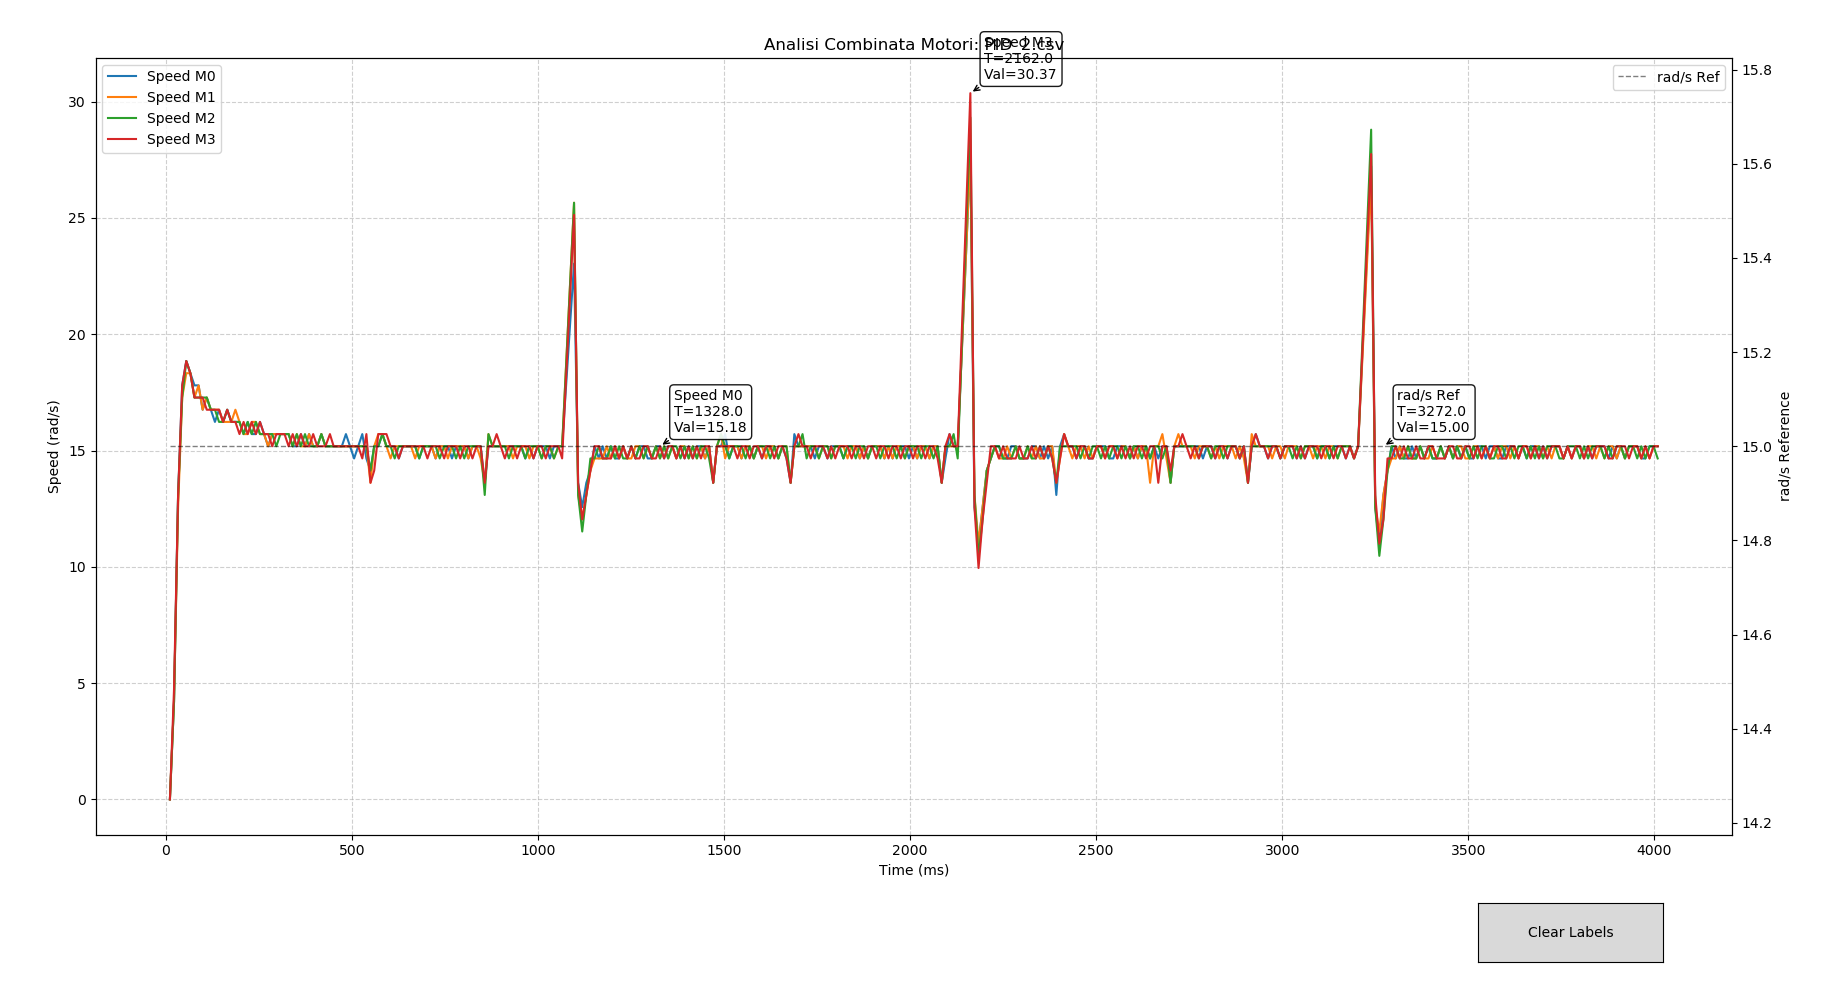
\includegraphics[width=1\textwidth]{IMG/PID/PID_15Rad_200hz_Feedforward_CloseLoop.png}
    \caption{Full closed-loop PID test at 15 rad/s (200 Hz) with Feedforward compensation}
    \label{fig:PID_15Rad_200hz_FF}
\end{figure}

\begin{figure}[H]
    \centering
    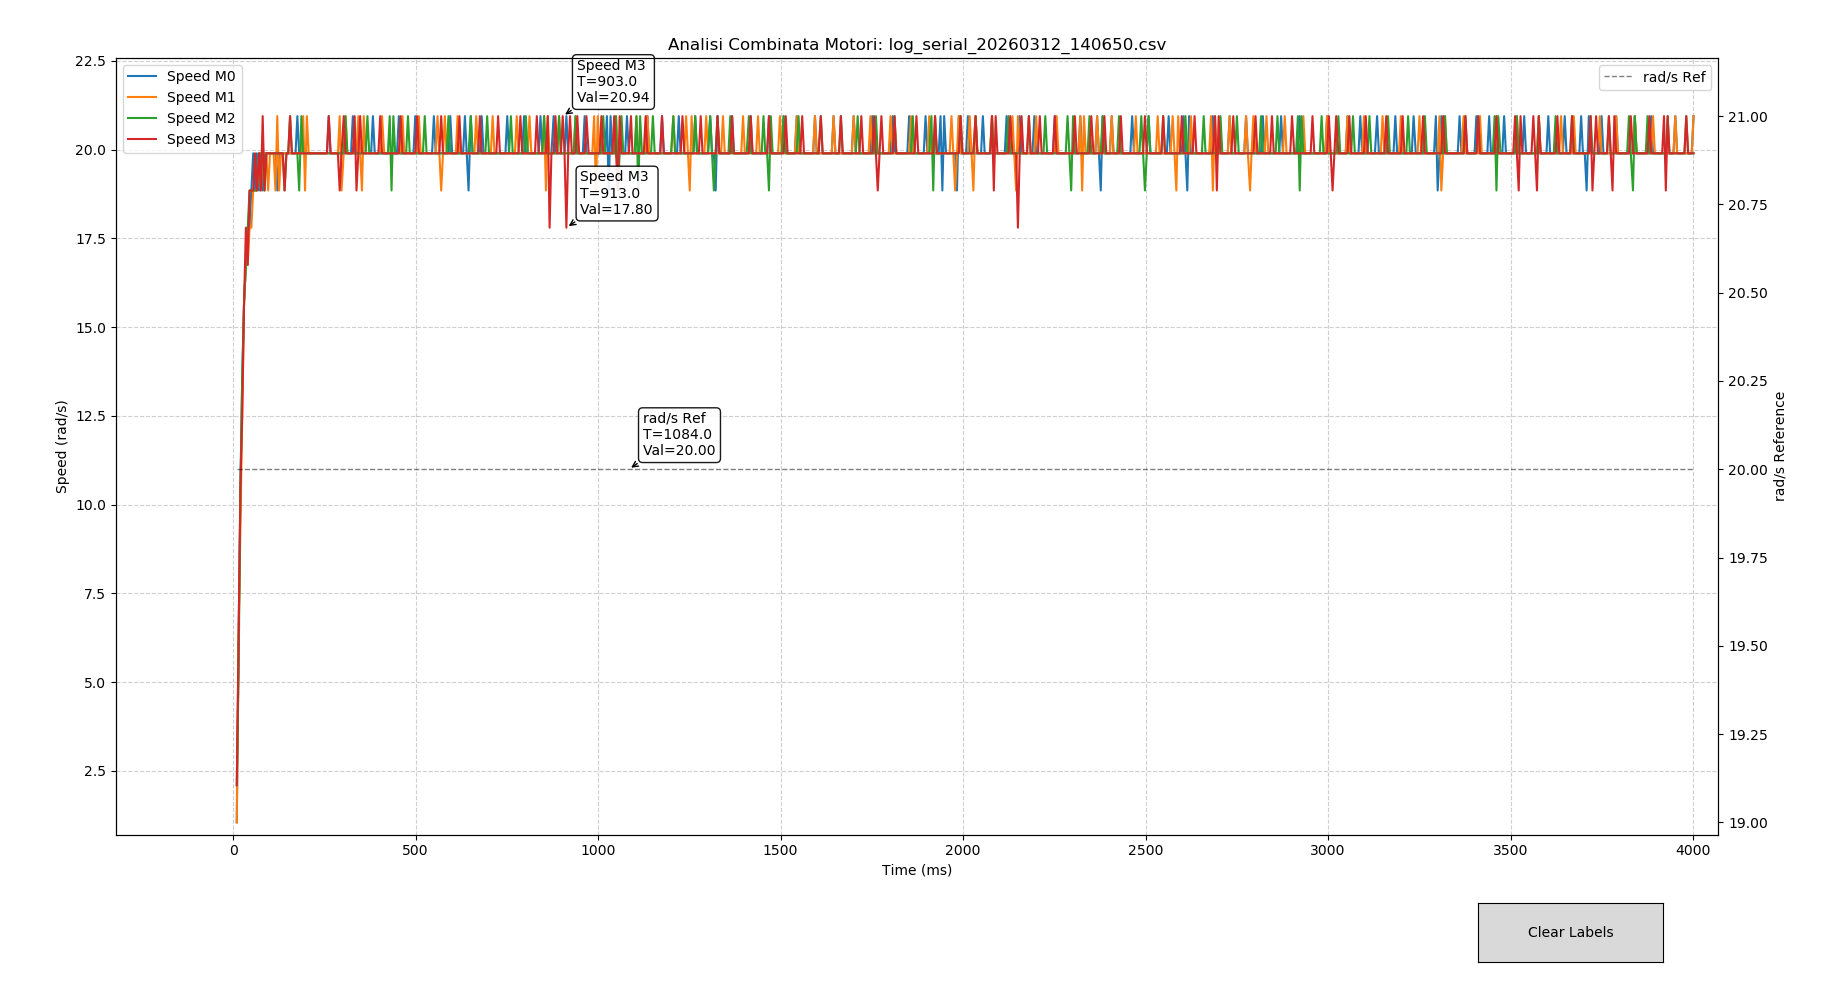
\includegraphics[width=1\textwidth]{IMG/PID/PID_20Rad_100hz_NoFeedforward_CloseLoopHalf.png}
    \caption{PID closed-loop response at 20 rad/s (100 Hz) showing increased measurement jitter}
    \label{fig:PID_20Rad_100hz_NoFF}
\end{figure}

\begin{figure}[H]
    \centering
    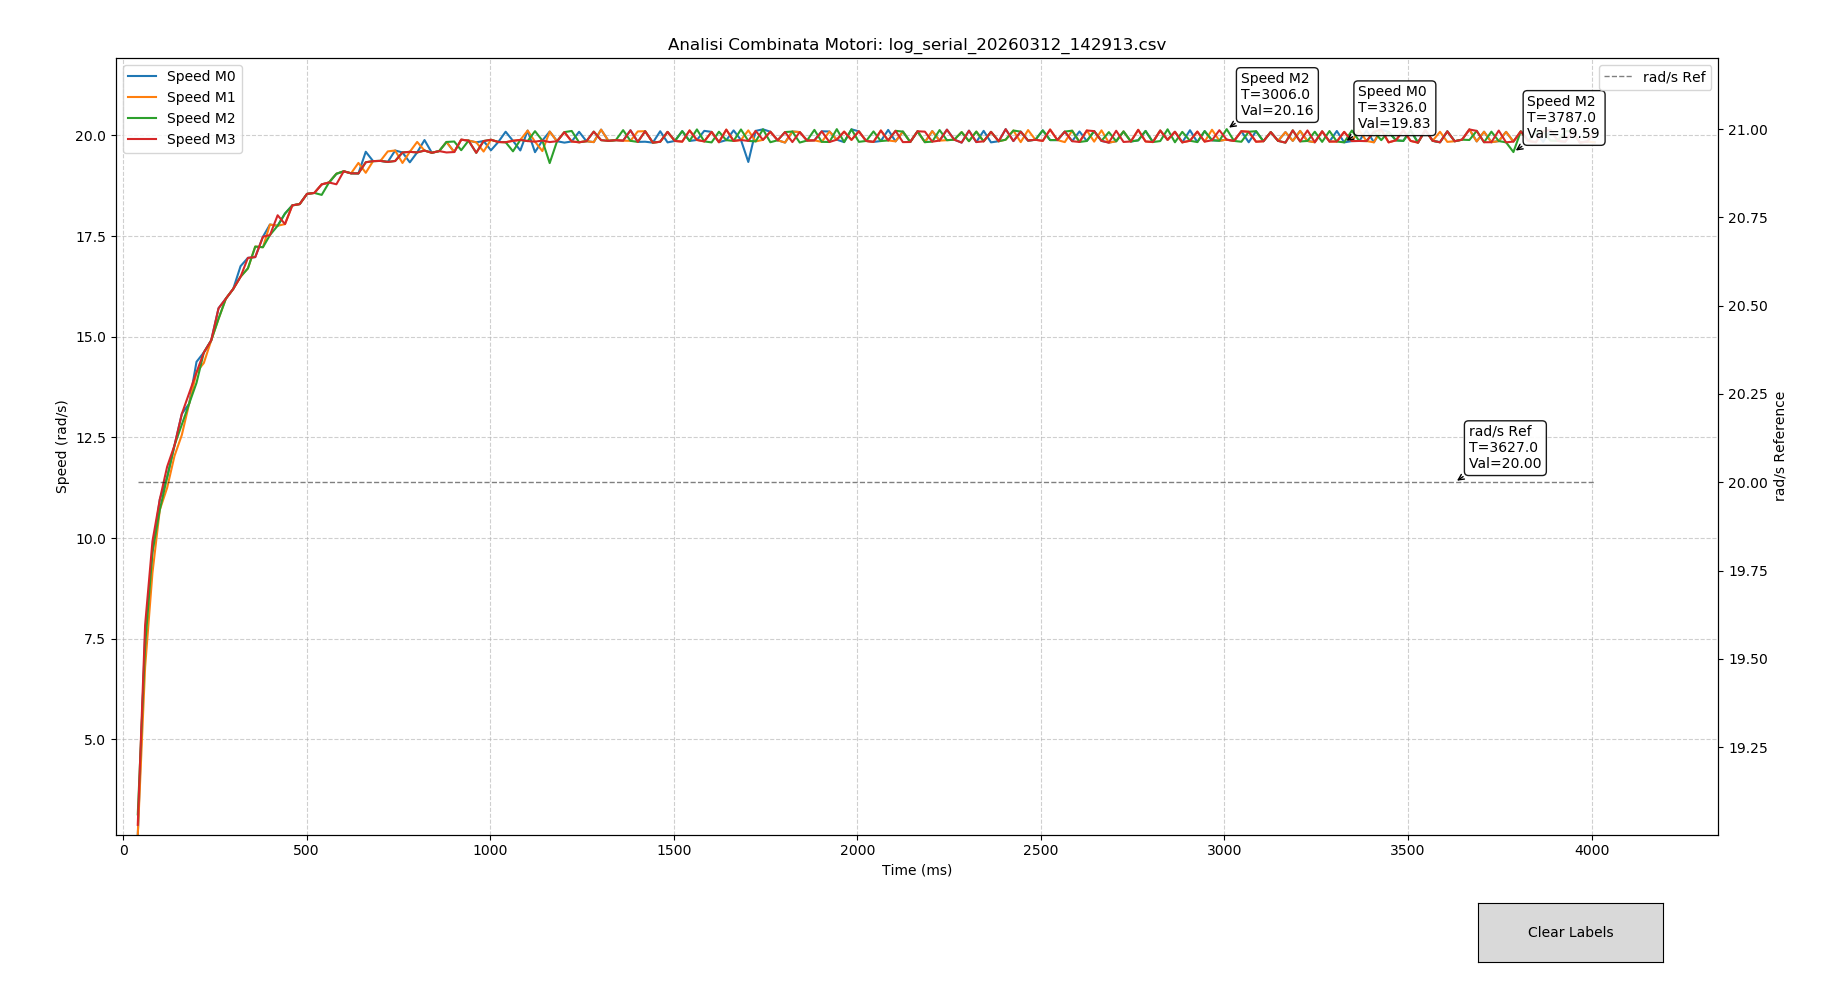
\includegraphics[width=1\textwidth]{IMG/PID/PID_20Rad_50hz_NoFeedforward_CloseLoopHalf.png}
    \caption{PID closed-loop tracking at 20 rad/s (50 Hz) without Feedforward}
    \label{fig:PID_20Rad_50hz_NoFF}
\end{figure}


 
\chapter{Omnicar Platform, ROS Integration and High-Level Software Architecture }

  \section{High-Level Software Architecture: From ROS1 Noetic to ROS2 Jazzy}
  In this thesis, the previous ROS1-based architecture was progressively migrated to ROS2 Jazzy.
  The objective wasn't to update the software stack, but also to obtain a structure that could be tested more easily, extended with new modules, and maintained on the Raspberry Pi 5.

  The transition to ROS2 was particularly relevant for this platform because the high-level software has to coordinate several modules: the serial driver, the odometry node, the localization pipeline, the lidar interface, and the motion-control nodes. In this context, the \textbf{Data Distribution Service} based communication layer of ROS2 provides a more suitable basis for distributed execution and future extensions than the previous centralized \textbf{ROS Master}.

  The hardware upgrade to the \textbf{Raspberry Pi 5} was also an important part of the migration. Compared with the \textbf{Raspberry Pi 3} used in the previous version, the new board offers more computational margin for running several ROS2 nodes at the same time. This is especially useful for odometry computation, localization, lidar data processing, and high-level control tasks, where delays or CPU saturation can directly affect the quality of the robot behaviour.

  \subsection{Migration and Local Implementation}
  From a practical point of view, the migration required rebuilding the software stack around the ROS2 workflow and checking each module separately before running the complete robot. This was necessary because the driver, odometry, localization, and control nodes depend on each other, but failures in one layer can easily mask problems in the others.

  During the migration, I chose to keep the project inside a dedicated ROS2 workspace on the Raspberry Pi instead of mixing the packages with system-level software. This made the development process easier to control, especially when rebuilding packages, changing configuration files, or testing only a subset of the nodes.

  \begin{itemize}
      \item \textbf{Dependency Isolation}: A local workspace allows better control
  of project-specific dependencies and reduces conflicts with system-wide
  libraries and packages.
      \item \textbf{Package organization}: The workspace structure helps organize drivers,
  interfaces, launch files, and configuration files in a clear and maintainable
  way.
      \item \textbf{Reproducibility}: The complete software can be deployed more
  easily on different Raspberry Pi boards while preserving the same internal
  package organization.
      \item \textbf{Future Extensions}: ROS2 makes future extensions easier, such as
  improved localization, additional sensors, and more advanced control features.
  \end{itemize}

  The migration was not limited to a simple syntax update. Some technical points
  required particular attention during the transition:

  \begin{itemize}
      \item the change from the ROS1 \texttt{catkin} build system to the ROS2
  \texttt{ament\_cmake} and \texttt{colcon} workflow;
      \item the adaptation of legacy custom messages and services to the ROS2
  interface package \texttt{sdpo\_drivers\_interfaces};
      \item the conversion of launch files to the ROS2 Python-based launch system;
      \item the verification of topic names, node names, parameter files, and TF
  frame conventions;
      \item the preservation of compatibility with the serial protocol used by the
  ESP32 firmware.
  \end{itemize}

  For this reason, the migration was performed progressively. I first focused on the ROS2 driver, because it represented the mandatory bridge between the Raspberry Pi and the ESP32 firmware. Once this communication layer was stable, the remaining modules could be migrated and tested one at a time.

  \subsection{Workspace Structure}
  The active ROS2 workspace of the project is \texttt{omnicar\_ws}. It follows the
  standard ROS2 and \texttt{colcon} organization, where the compiled artifacts are
  separated from the source code. In particular, the directories \texttt{build/},
  \texttt{install/}, and \texttt{log/} contain the compilation results and runtime
  environment, while the \texttt{src/} directory contains the software packages
  under development.

  Each package keeps the standard ROS2 files, namely \texttt{CMakeLists.txt} and \texttt{package.xml}, which define the build targets, dependencies, and package metadata.

  The separation between header files (\texttt{.h}) and source files
  (\texttt{.cpp}) remains important for code organization and maintainability.
  Header files define the interfaces of the software components, while source
  files implement the internal logic. This structure simplifies development and
  supports incremental compilation.

  The \texttt{config} directories use \texttt{.yaml} files to store parameters
  such as communication settings, odometry constants, and localization
  configuration. This choice makes the system easier to configure and tune without
  modifying the source code.

  The following directory tree shows the simplified structure of the active ROS2
  workspace:

\begin{folderbox}{omnicar\_ws: Simplified Structure}
\begingroup
\scriptsize
\renewcommand{\baselinestretch}{0.85}\selectfont
\dirtree{%
.1 omnicar\_ws/.
.2 bags/ \DTcomment{Recorded ROS2 bag files from controller and robot tests}.
.2 Test/ \DTcomment{Offline analysis workspace for experimental validation}.
.3 test\_code/ \DTcomment{Python scripts and configuration files for bag analysis}.
.3 test\_results/ \DTcomment{Generated plots, metrics and summaries from test runs}.
.2 src/ \DTcomment{ROS2 source workspace containing robot packages and support libraries}.
.3 5dpo\_ratf\_driver-main/ \DTcomment{Main ROS2 robot driver package}.
.4 include/ \DTcomment{Header files for robot and driver classes}.
.4 src/ \DTcomment{ROS2 source files, including driver and tuning nodes}.
.4 launch/ \DTcomment{ROS2 launch files, including bringup}.
.4 sh/ \DTcomment{Support scripts and legacy tuning utilities}.
.3 sdpo\_driver\_omnijoy/ \DTcomment{ROS2 joystick teleoperation node}.
.4 src/ \DTcomment{Joystick command processing logic}.
.4 launch/ \DTcomment{Launch file for Logitech F710 teleoperation}.
.3 sdpo\_drivers\_interfaces/ \DTcomment{ROS2 custom messages and services}.
.4 msg/ \DTcomment{Motor reference and encoder feedback messages}.
.4 srv/ \DTcomment{Custom service definitions}.
.3 sdpo\_ros\_odom/ \DTcomment{ROS2 odometry computation package}.
.4 include/ \DTcomment{Odometry class headers}.
.4 src/ \DTcomment{Odometry implementation}.
.4 config/ \DTcomment{Kinematic and wheel parameters}.
.4 launch/ \DTcomment{Odometry launch files}.
.3 sdpo\_ratf\_ros\_localization/ \DTcomment{ROS2 localization module}.
.4 include/ \DTcomment{Localization and EKF headers}.
.4 src/ \DTcomment{Localization implementation}.
.4 config/ \DTcomment{Localization parameters}.
.4 launch/ \DTcomment{Localization launch file}.
.3 ldlidar\_stl\_ros/ \DTcomment{ROS2 lidar integration package}.
.4 src/ \DTcomment{Lidar publishing and listening nodes}.
.4 config/ \DTcomment{Lidar configuration files}.
.3 5dpo\_serial\_port-main/ \DTcomment{Asynchronous serial communication library}.
.4 include/ \DTcomment{Serial communication headers}.
.4 src/ \DTcomment{Async serial implementation}.
.3 serial\_communication\_channels-main/ \DTcomment{Serial channel protocol library}.
.4 include/ \DTcomment{Protocol headers}.
.4 src/ \DTcomment{Protocol implementation}.
.3 sdpo\_motion\_control/ \DTcomment{High-level ROS2 motion-control package}.
.4 config/ \DTcomment{Controller parameter files and trajectory/path settings}.
.4 src/ \DTcomment{Controller node implementations for go-to-point and path following}.
.4 launch/ \DTcomment{Launch files for controller tests}.
.4 msg/ \DTcomment{Custom debug messages published by the control nodes}.
}
\endgroup
\end{folderbox}



 \subsection{Experimental Validation: ROS2 Integration and Control Chain}
  This phase of the software integration focused on validating the
  communication and control chain of the OmniCar platform in the ROS2 environment.
  These tests were intended to verify the correctness of serial communication with
  the ESP32 controller, the consistency of encoder feedback, joystick commands, odometry, and localization modules inside the migrated ROS2 architecture.

  \subsubsection{Test 1: Encoder Monitoring and Open-Loop Velocity Control}
  The first test was intentionally simple, because before testing odometry or control it was necessary to verify that the Raspberry Pi could receive reliable encoder data from the ESP32.

  \paragraph{Operational Procedure}
  After enabling access to the serial device, the main driver node,
  \texttt{sdpo\_ratf\_driver}, was launched. This node is the central
  communication interface between the ROS2 graph and the ESP32 firmware. In the
  current implementation, it subscribes to the \texttt{motors\_ref} topic and
  publishes encoder and digital state feedback through the topics
  \texttt{motors\_enc}, \texttt{switch\_1\_state}, and \texttt{switch\_2\_state}.
  
  \vspace{0.2cm}
  
  To validate the feedback chain, the \texttt{motors\_enc} topic was monitored
  during runtime while the wheels were rotated manually. This check confirmed the
  correct reception of encoder increments, the absence of packet loss, and the
  correct transmission of angular speed and ticks-per-revolution information from
  the embedded layer to ROS2.

  \vspace{0.2cm}
  
  For actuation validation, a constant reference was sent on the
  \texttt{motors\_ref} topic using the custom message type
  \texttt{sdpo\_drivers\_interfaces/msg/MotRefArray}. In this way, it was possible
  to verify the complete command path from ROS2 to the ESP32 firmware.

  The test confirmed that the node \texttt{sdpo\_ratf\_driver} acts as the central
  bridge of the low-level architecture. It guarantees bidirectional data exchange
  with the embedded controller while providing a stable interface for the higher-
  level ROS2 nodes.

\begin{figure}[H]
    \centering
    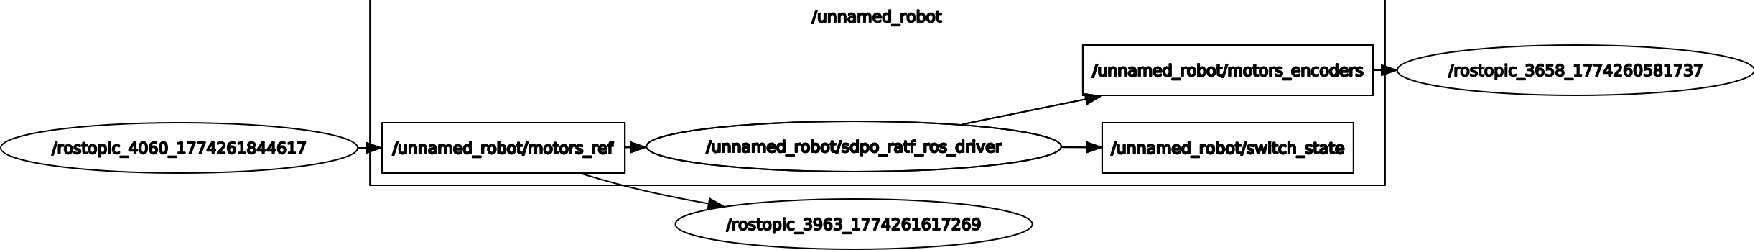
\includegraphics[width=1.1\textwidth]{IMG/ROS/PDF_rosgraph_test_enc_vel_ref.pdf}
    \caption{rqt\_graph showing the active nodes and topics during the encoder test, including reference velocity and measured encoder feedback.}
    \label{fig:rqt_graph_test_Encoder}
\end{figure}

\begin{vscode}{Commands to use for Test 1}
CMD1  
  ros2 launch sdpo_ratf_driver sdpo_ratf_driver.launch.py

CMD2
  ros2 topic echo /unnamed_robot/motors_enc

CMD3
  ros2 topic pub -r 20 /unnamed_robot/motors_ref sdpo_drivers_interfaces/msg/MotRefArray "{ang_speed_ref: [{ref: 5.0}, {ref: 5.0}, {ref: 5.0}, {ref:5.0}]}"
  ros2 topic pub -r 20 /unnamed_robot/motors_ref sdpo_drivers_interfaces/msg/MotRefArray "{ang_speed_ref: [{ref: 0.0}, {ref: 0.0}, {ref: 0.0}, {ref:0.0}]}"
\end{vscode}

  \subsubsection{Test 2: Manual Control using a Joystick Controller}
  The second validation phase concerned the integration of a joystick controller
  in the ROS2 environment, with the aim of verifying manual control of the
  platform and the correct interaction between high-level user commands and low-
  level motor actuation.

  The teleoperation chain is organized into three stages:
  \begin{itemize}
      \item \textbf{Joystick Acquisition}: The node \texttt{joy\_linux\_node},
  launched through the package \texttt{joy\_linux}, acquires the state of the
  Logitech F710 controller and publishes it on the topic \texttt{joy} as
  \texttt{sensor\_msgs/msg/Joy}.
      \item \textbf{User Command Interpretation}: The node
  \texttt{sdpo\_driver\_omnijoy} subscribes to \texttt{joy} and converts the
  joystick inputs into a velocity command of type \texttt{geometry\_msgs/msg/
  Twist}, published on the topic \texttt{cmd\_vel}. This node applies deadman
  logic and scaling factors for linear and angular motion.
      \item \textbf{Conversion into Wheel References}: The node
  \texttt{sdpo\_ros\_odom\_cmd\_vel} subscribes to \texttt{cmd\_vel}, applies the
  inverse kinematics of the four-wheel omnidirectional platform, and publishes the
  resulting wheel references on \texttt{motors\_ref}. In addition, it publishes
  the scaled robot-level reference on \texttt{cmd\_vel\_ref}.
  \end{itemize}

  At this point, the node \texttt{sdpo\_ratf\_driver} receives the
  \texttt{motors\_ref} message and transmits the corresponding angular speed
  references to the ESP32 firmware through the serial communication protocol.

  This result is important, because it shows that the migrated ROS2 control chain is modular and separated into functional layers. The joystick node manages the user input, the kinematic conversion node computes the wheel references, and the main driver handles
  communication with the embedded controller. This separation improves clarity,
  maintainability, and testability of the overall system.

  \begin{figure}[H]
    \centering
    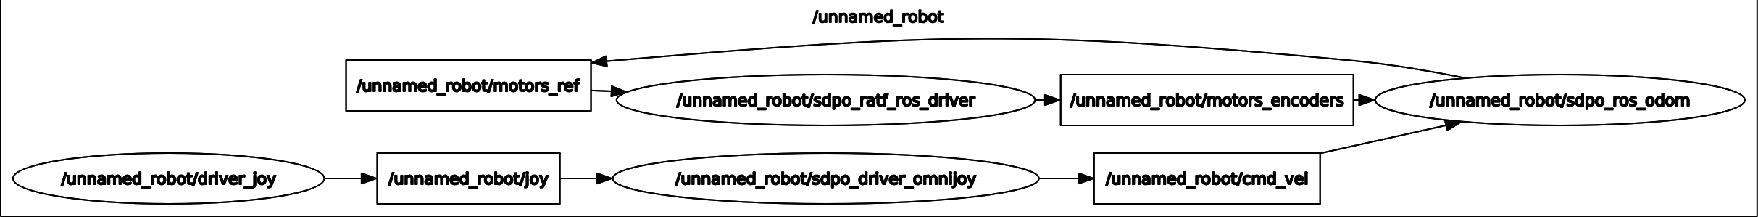
\includegraphics[width=1.1\textwidth]{IMG/ROS/PDF_rosgraph_test_joystick.pdf}
    \caption{rqt\_graph showing the active nodes and topics during the joystick test}
    \label{fig:rqt_graph_test_joy}
\end{figure}

\begin{vscode}{Commands to use for Test 2}
CMD 1
ros2 launch sdpo_ratf_driver omnicar_joy_control.launch.py

CMD 2
ros2 topic echo /unnamed_robot/odom
\end{vscode}

\vspace{0.4cm}

  \subsubsection{Test 3: Localization and Lidar Integration}
  After validating the joystick teleoperation chain, the next step was to verify that the odometry node produced a coherent estimate of the robot motion. The robot was moved manually or through joystick commands while the estimated pose and TF frames were observed in RViz. The comparison with the real motion showed that the direction of motion and frame alignment were consistent, although small discrepancies appeared due to wheel slip, odometric drift, and modelling errors.

  \vspace{0.2cm}
  
  The localization function is managed by the node
  \texttt{sdpo\_ratf\_ros\_localization}, which subscribes to \texttt{odom} and,
  when enabled, also to \texttt{laser\_scan\_point\_cloud}. It publishes the
  estimated robot pose on the topic \texttt{pose}, the detected beacons on
  \texttt{beacons}, and the reference map beacons as \texttt{map\_beacons}.
  Moreover, it broadcasts the TF transform between the frames \texttt{map} and
  \texttt{odom}.

\vspace{0.2cm}

  This architecture allows localization to refine the odometric estimate by
  combining wheel-based motion prediction with external observations derived from
  the lidar subsystem.
  The localization process can be observed in Fig.~\ref{fig:odom_comparison}, where the RViz visualization shows the lidar scan in red and the detected beacons in white, providing a direct representation of the perception layer used for pose estimation.

\vspace{0.2cm}

  The TF tree adopted in this configuration follows the standard chain \newline 
  \texttt{map} $\rightarrow$ \texttt{odom} $\rightarrow$ \texttt{base\_footprint} $\rightarrow$ \texttt{laser}.
  
   \newline  
   
  In this structure, the \texttt{map} frame represents the global reference, \texttt{odom} provides a continuous but drifting local estimate, \texttt{base\_footprint} defines the robot base frame, and \texttt{laser} corresponds to the lidar sensor frame. This hierarchical organization ensures consistency between localization, odometry, and sensor measurements.

\vspace{0.2cm}

  The lidar integration is provided by the package \texttt{ldlidar\_stl\_ros},
  which publishes scan data for the perception layer. In the current migration
  process, the lidar is an important component because it supports the
  localization pipeline and extends the ROS2 stack beyond basic low-level control.

  The comparison between the real experiment and the RViz visualization shows that the odometry provides a consistent estimate of the robot motion. The trajectory and frame alignment are coherent, while small differences are due to odometric drift, wheel slip, and modeling errors.
  For the following Test, the same laucher used in the previous test is valid.

 \begin{figure}[H]
    \centering

    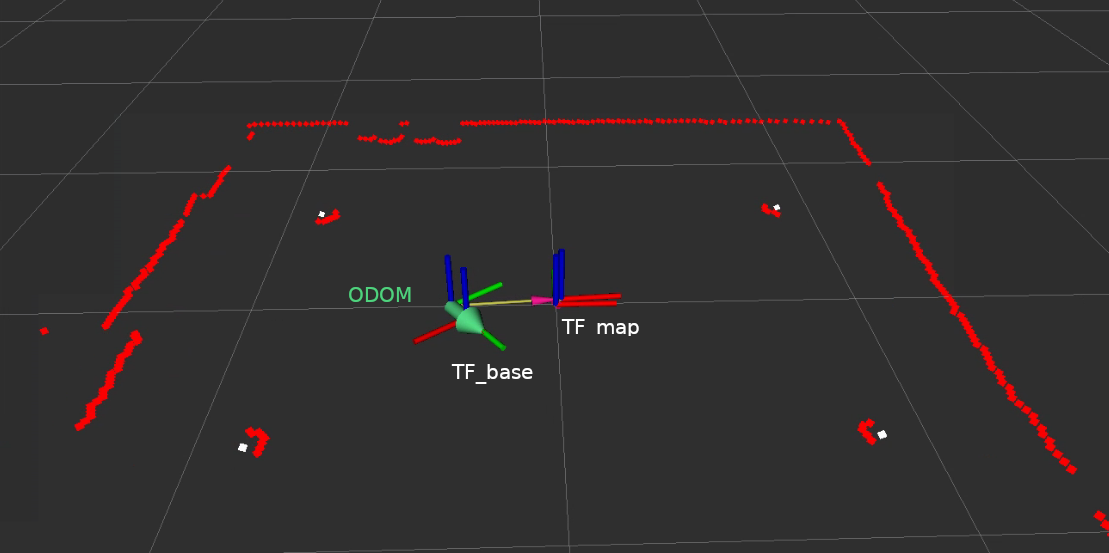
\includegraphics[width=0.90\linewidth]{IMG/ROS/rviz2_odom_edit.png}
    \caption*{RViz odometry and TF visualization}

    \vspace{0.4cm}

    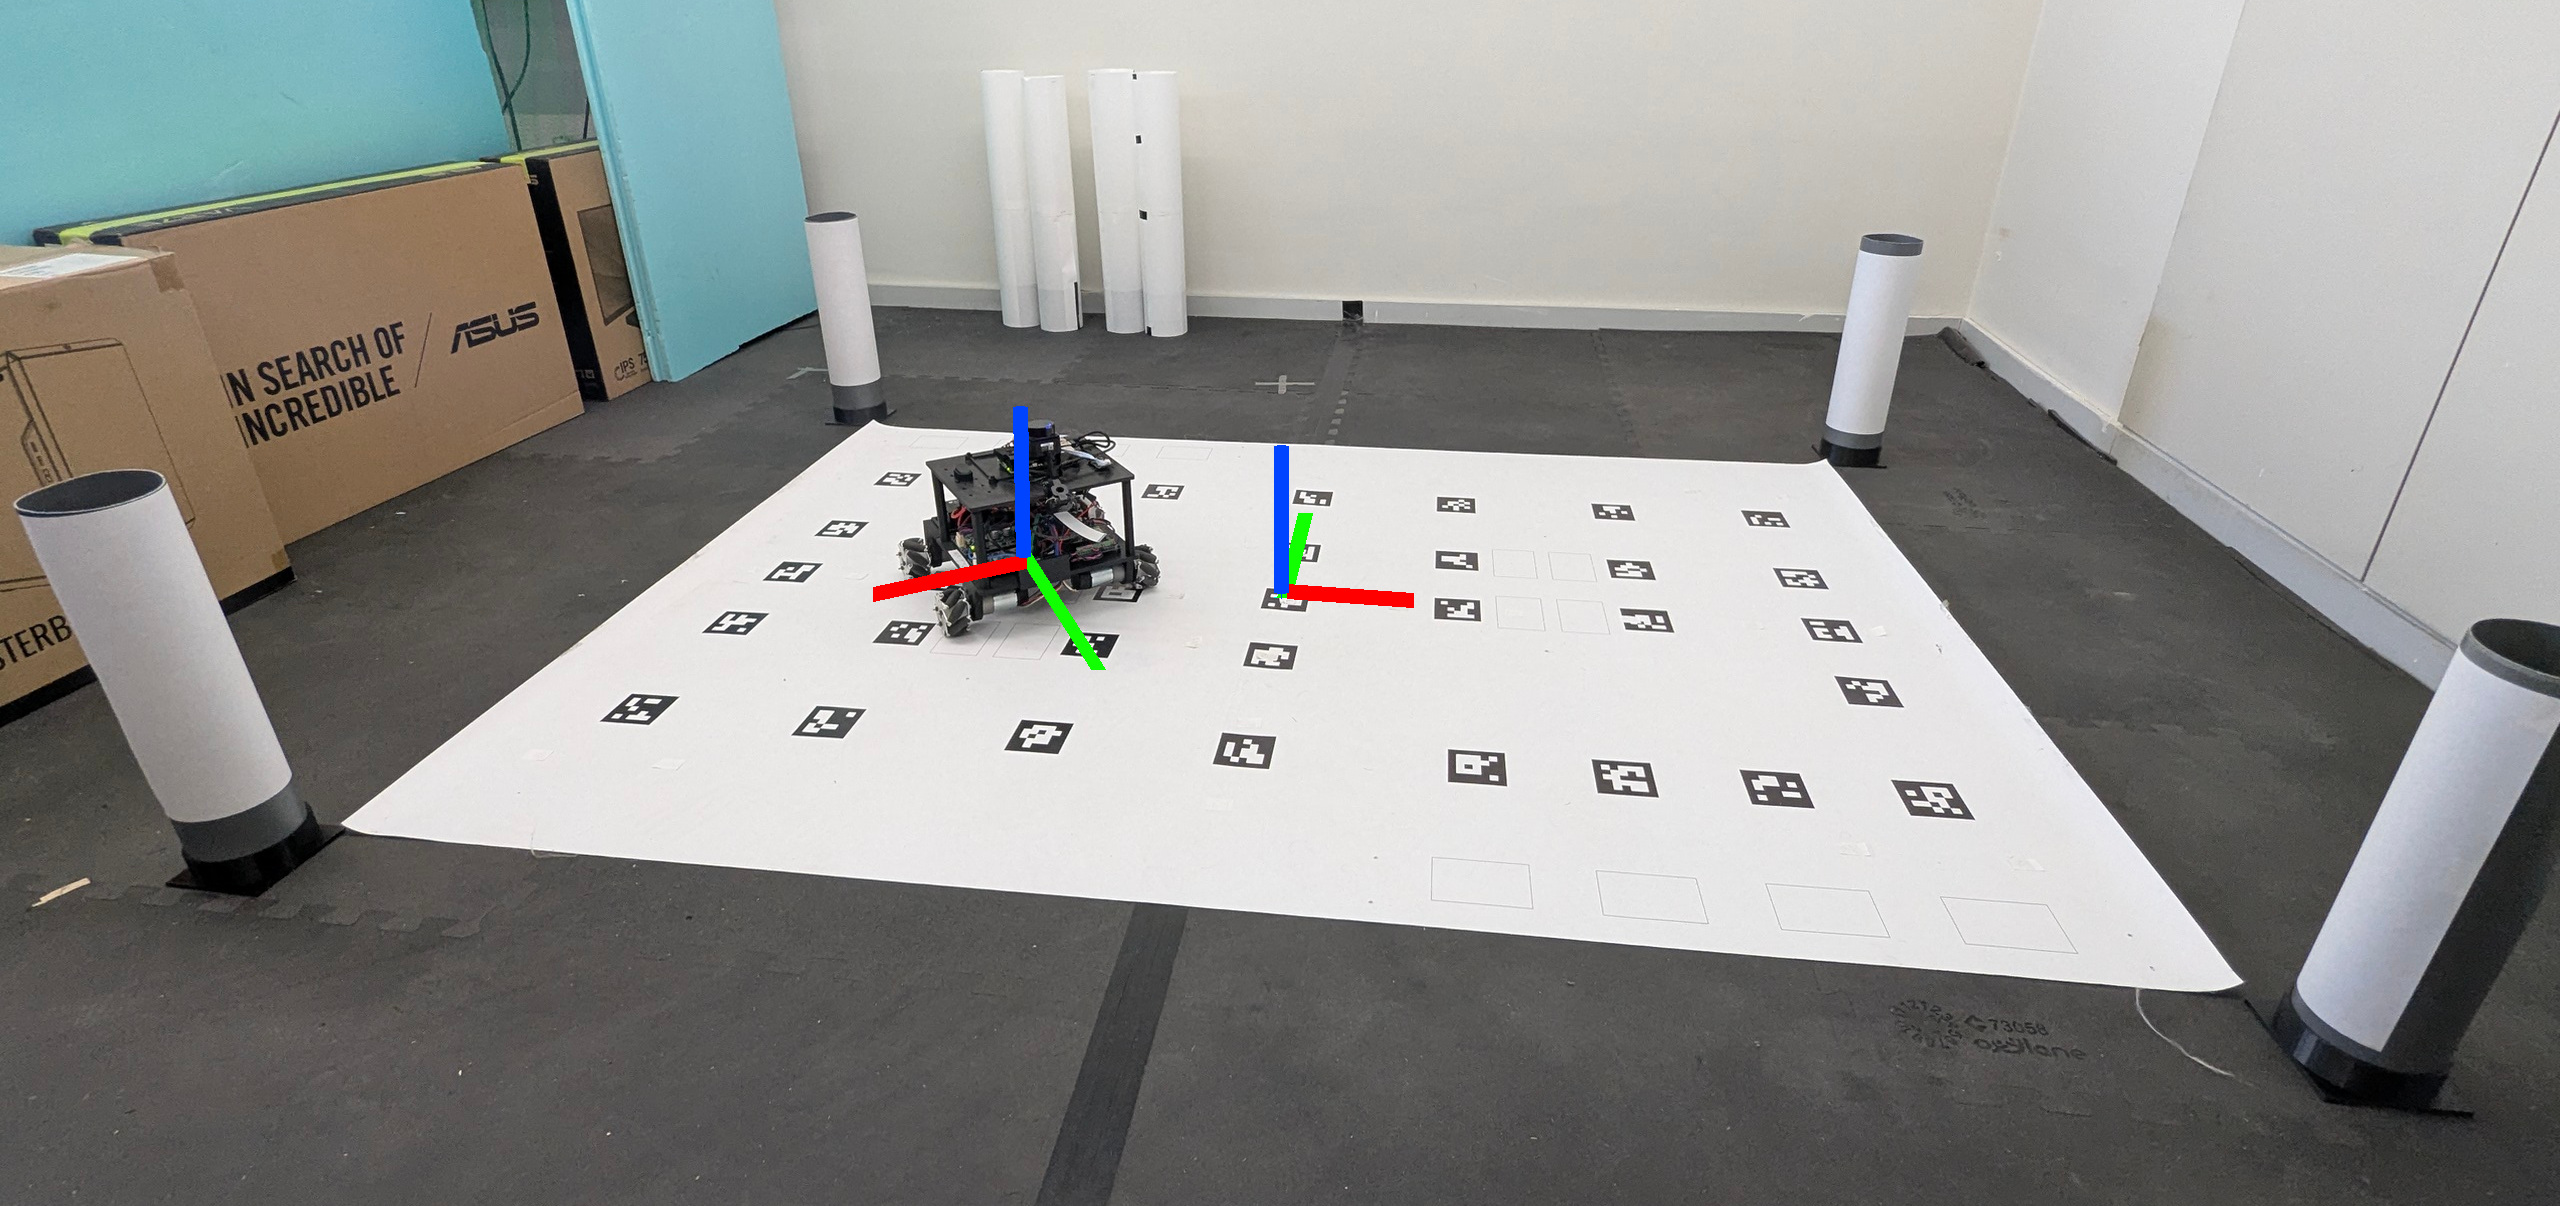
\includegraphics[width=0.90\linewidth]{IMG/ROS/odom_real_edit.jpg}
    \caption*{Real experimental setup}

    \caption{Comparison between the real robot experiment and the corresponding odometry visualization in RViz.}
    \label{fig:odom_comparison}
\end{figure}


\newpage
\subsubsection{Test 4: Waypoint Tracking Validation with the
  \texttt{go\_to\_point} Controller}

  This test represented the first closed-loop high-level motion-control experiment performed within the migrated ROS2 architecture. In this phase, the package \texttt{sdpo\_motion\_control} was used to command the robot toward a
  sequence of planar target poses, with the objective of evaluating the behaviour of the \texttt{go\_to\_point} controller, the consistency of the odometric feedback, and the overall quality of the integrated control chain.

\vspace{0.4cm}

  This test was carried out after correcting an inconsistency in the
  \texttt{map}--\texttt{odom} transformation inside the localization chain. In
  the previous implementation, the rotation between \texttt{map} and \texttt{odom}
  was computed correctly, but the translation term was combined with the robot EKF
  yaw instead of the relative \texttt{map}--\texttt{odom} rotation. This produced a
  frame inconsistency. After this correction, the waypoint experiments became coherent and repeatable.

  \paragraph{Test configuration}
  For controller tuning and validation, six reference poses were assigned in
  sequence. The same six target positions are the ones shown in the plots of
  target trajectory, current robot trajectory, and tracking errors:
  
\begin{figure}[H]
    \centering
    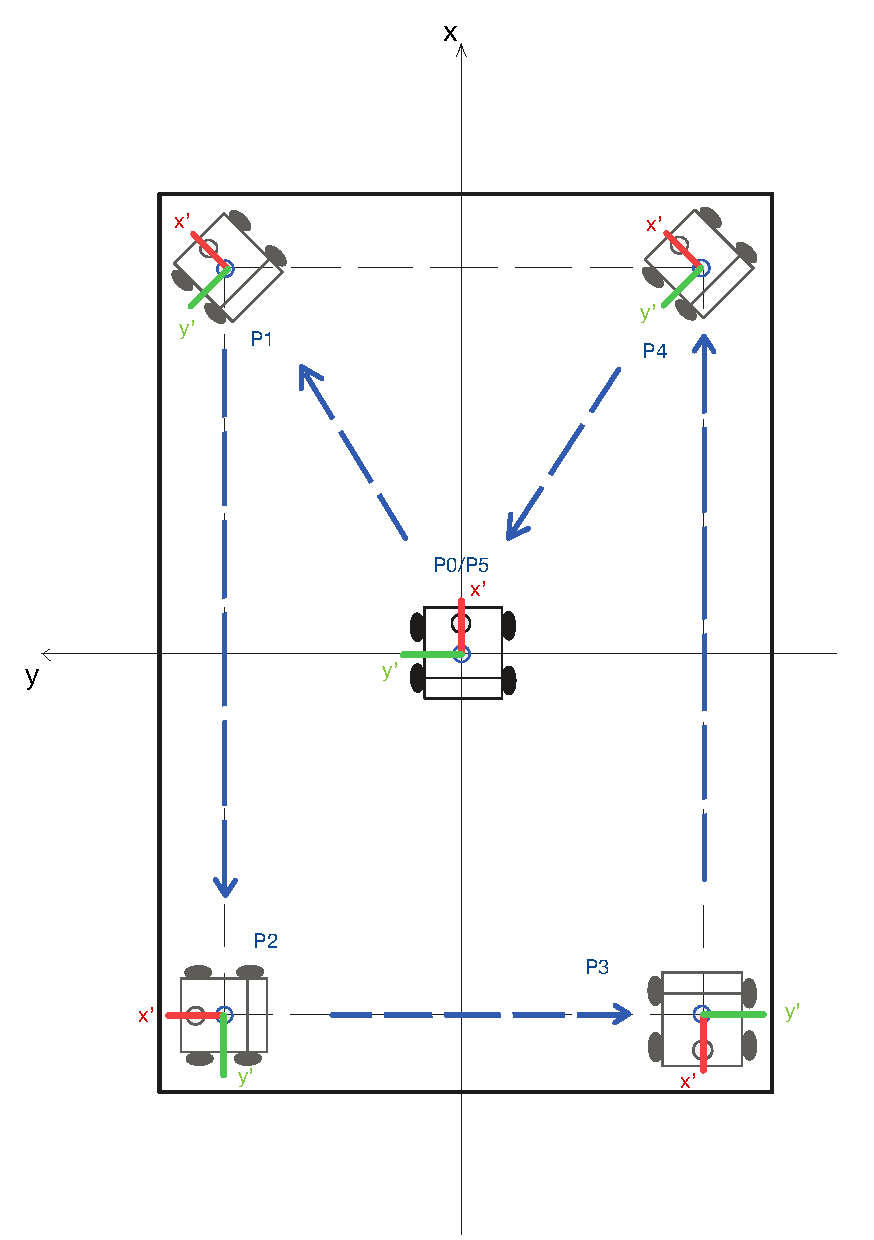
\includegraphics[width=0.52\textwidth]{IMG/ROS/GoToPoint_test_Draw.pdf}
    \caption{diagram of the test executed}
    \label{fig:GoToPoint_test}
\end{figure}

\begin{itemize}
  \item \texttt{(P0) \{x: 0.0, y: 0.0, z: 0.0\}}
  \item \texttt{(P1) \{x: 0.6, y: 0.45, z: 0.78\}}
  \item \texttt{(P2) \{x: -0.6, y: 0.45, z: 1.56\}}
  \item \texttt{(P3) \{x: -0.6, y: -0.45, z: 3.14\}}
  \item \texttt{(P4) \{x: 0.6, y: -0.45, z: 0.78\}}
  \item \texttt{(P5) \{x: 0.0, y: 0.0, z: 0.0\}}
\end{itemize}

    The sequence was chosen to force the robot to move in different directions of the workspace, including diagonal displacements where odometric errors and wheel slip are more visible, ending with a return to the origin.

  \paragraph{Observed behaviour}
  The experiments showed that the \texttt{go\_to\_point} controller is able to
  drive the robot through the assigned sequence and to reach all the commanded
  poses with stable behaviour. Motions along the main axes were generally more
  accurate.

\begin{figure}[H]
    \centering
    \includegraphics[width=1.0\textwidth]{IMG/ROS/TEST4_position.png}
    \caption{plot control position results}
    \label{fig:TEST4_position}
\end{figure}

\begin{figure}[H]
    \centering
    \includegraphics[width=1.0\textwidth]{IMG/ROS/TEST4_position_error.png}
    \caption{plot position errors}
    \label{fig:TEST4_position_error}
\end{figure}

  The comparison between the commanded target pose and the estimated current pose,
  together with the plots of the tracking error, highlighted that the control loop
  remained stable during all tests, but also confirmed the presence of a
  residual positioning error. Over the waypoint sequence, the largest observed deviation was on the order of \(2 \ \mathrm{cm}\) on each
  axis. This discrepancy was not mainly associated with instability of the
  controller itself, but rather with the accumulated estimation error of the
  pose used by the controller.

  The results were particularly useful because they helped separate the effect
  of
  control tuning from the effect of state estimation. In fact, the tests
  confirmed
  that the basic control chain
  \texttt{goal} $\rightarrow$ \texttt{controller} $\rightarrow$
  \texttt{cmd\_vel}
  $\rightarrow$ \texttt{motors\_ref} $\rightarrow$ robot is functionally
  correct,
  while the main limitation at this stage is the residual drift and bias of the
  pose estimate over longer or diagonal displacements.

  \paragraph{Discussion of the results}
  From a control point of view, these experiments represent the first successful
  validation of waypoint regulation in the migrated ROS2 architecture. The robot
  was able to execute repeated planar repositioning tasks using the new
  \texttt{sdpo\_motion\_control} package, and the obtained behaviour is already
  sufficient to consider the controller as a valid baseline for further tuning
  and for future trajectory-tracking developments.

  At the same time, the tests showed that improved precision will require not
  only controller tuning, but also a more accurate calibration of the localization
  and odometry chain, especially for diagonal motions and global return-to-origin
  tasks. For this reason, Test~4 was an important milestone: it validated the
  complete waypoint control loop in ROS2 and clearly identified the remaining
  gap between acceptable closed-loop operation and higher-accuracy autonomous
  navigation.

  \subsection{Final Considerations on the Integrated ROS2 Chain}
From a control perspective, the \texttt{go\_to\_point} validation was carried out within a cascaded control architecture, where the inner loop was already introduced in the previous chapters.

At the embedded level, the ESP32 firmware implements the low-level wheel-velocity regulation loop, including the motor control logic discussed in Chapter~\ref{chap:firmware}. This inner loop tracks wheel-speed references and provides the actuation layer required by the ROS2 motion stack. As a result, the high-level controller running on the Raspberry Pi can be designed at the robot-motion level, in terms of planar pose regulation.

\begin{figure}[H]
    \centering
    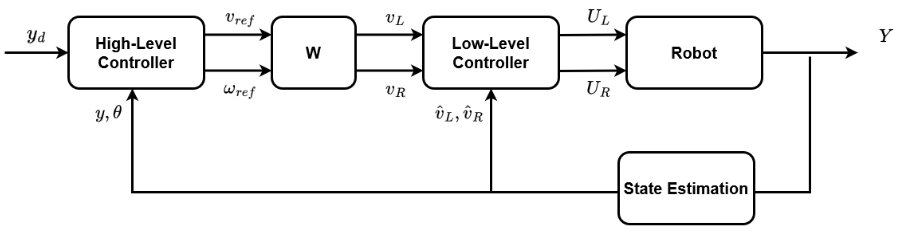
\includegraphics[width=1.0\textwidth]{IMG/controller/controller_general_architecture.png}
    \caption{Controller Architecture}
    \label{fig:Control_Architecture}
\end{figure}

Motion-control architecture adopted for OMNICAR as a two-layer cascade, consistent with the firmware and ROS2 integration described in the previous chapters.

\begin{itemize}
\item \textbf{High-level controller}: receives the estimated robot pose \((x,y,\theta)\) from the state-estimation pipeline and computes robot-level reference velocities for motion tasks (initially waypoint regulation, later path-following scenarios). These references are then mapped to wheel-level commands through the kinematic transformation block \(W\).

\item \textbf{Low-level controller}: implemented on the ESP32, receives wheel-velocity references and applies closed-loop motor control to track them through PWM/DIR actuation, using encoder feedback for regulation.
\end{itemize}

This architecture, shown in Fig.~\ref{fig:Control Architecture}, provides a clear separation of responsibilities: high-level motion generation in ROS2 and fast embedded actuation at firmware level. In the present chapter, the high-level scenario is limited to a \texttt{go\_to\_point} task with a P-only outer loop.

In the ROS2 experiments presented in Test~4, the high-level outer loop was intentionally kept simple and implemented as a \textbf{P-only controller} on the planar coordinates \((x,y,\psi)\). Three proportional actions were used to generate the commanded robot velocities from position and heading errors, while integral and derivative terms were disabled in this phase.

The tuning was performed progressively by starting from moderate proportional gains (around \(K_p \approx 0.8\), then adjusted per axis) and increasing them until a satisfactory compromise between responsiveness and oscillation margin was obtained. This approach was chosen to obtain a robust baseline controller and to isolate the effect of the localization and odometry chain on the final positioning performance.

Experimental results confirmed that this P-only outer loop is sufficient to achieve stable waypoint reaching and repeatable closed-loop behavior for the considered trajectories. Residual errors, especially during diagonal motions and return-to-origin phases, were mainly associated with state-estimation drift and model mismatch rather than with instability of the proportional control law itself.

This test should therefore be interpreted as the first high-level control scenario in the migrated ROS2 architecture: a deliberately simple and transparent baseline. In the next chapter, more advanced high-level control scenarios will be analyzed.


  

 
\chapter{Motion Control Design and Experimental Evaluation}
\label{chap:motion_control_design}

The high-level control loop is implemented in ROS2 inside the package
\texttt{sdpo\_motion\_control}. Its role is to compute planar velocity commands
for the omnidirectional robot from the measured pose and from the desired path.
The output of this layer is a body-frame velocity command:
\begin{equation}
    \mathbf{u}
    =
    \begin{bmatrix}
        v_x & v_y & \omega
    \end{bmatrix}^{T},
\end{equation}
where \(v_x\) is the linear velocity component along the robot \(x_b\)-axis,
  \(v_y\) is the linear velocity component along the robot \(y_b\)-axis, and
  \(\omega\) is the yaw rate around the vertical axis. Therefore, \(v_x\) and
  \(v_y\) are not two independent wheel speeds, but the two planar components of
  the robot velocity in the body frame.


The robot pose in the global frame is defined as:
\begin{equation}
    \mathbf{x}
    =
    \begin{bmatrix}
        x & y & \psi
    \end{bmatrix}^{T},
\end{equation}
where \(x\) and \(y\) are the robot position and \(\psi\) is the yaw angle. The
controllers studied in this section are structured path-following controllers.
They do not directly solve an optimization problem. Instead, they use geometric
quantities such as path projection, path tangent, cross-track error, and
along-track error.

Two controllers are analysed:

\begin{itemize}
    \item the \textbf{Moving Reference proportional controller}, implemented as
    \texttt{moving\_reference\_p};
    \item the \textbf{Linear Segment controller}, implemented as
    \texttt{linear\_segment}.
\end{itemize}

For each controller, the control law, the main parameters, the test setup, the
quantitative results, and the experimental figures are reported.

\section{Evaluation Protocol and Metrics}
\label{sec:evaluation_protocol}

The experiments are evaluated using the recorded path-following datasets stored
in:

\begin{itemize}
    \item \texttt{Test/test\_results/RECTANGULAR\_test/};
    \item \texttt{Test/test\_results/}.
\end{itemize}

The main performance indicators are computed from the sampled tracking errors.
For a generic error signal \(e_i\), with \(N\) samples, the root mean square
error is:

The root mean square errot is:
\begin{equation}
    \mathrm{RMSE}_{e}
    =
    \sqrt{
        \frac{1}{N}
        \sum_{i=1}^{N} e_i^2
    }.
\end{equation}

The mean absolute error is:
\begin{equation}
    \mathrm{MAE}_{e}
    =
    \frac{1}{N}
    \sum_{i=1}^{N} |e_i|.
\end{equation}

The maximum absolute error is:
\begin{equation}
    e_{\max}
    =
    \max_{i=1,\dots,N} |e_i|.
\end{equation}

The path progression ratio is used to understand how much of the reference path
was covered during the test:
\begin{equation}
    r_{\gamma}
    =
    \frac{\gamma_{\mathrm{final}}}{L_{\mathrm{path}}},
\end{equation}
where \(\gamma_{\mathrm{final}}\) is the final curvilinear abscissa reached by
the reference or projection point, and \(L_{\mathrm{path}}\) is the total path
length. A value close to one means that the robot completed almost the whole
path.

The velocity saturation ratios are also reported:
\begin{equation}
    r_{\mathrm{sat},v_x}, \quad
    r_{\mathrm{sat},v_y}, \quad
    r_{\mathrm{sat},\omega}.
\end{equation}
These values indicate the fraction of samples in which the corresponding
velocity command reached its imposed limit.

\section{Moving Reference Proportional Controller}
\label{sec:moving_reference_controller}

\subsection{Control Principle}

The Moving Reference controller tracks a virtual point that moves along the
path. The path is described by a parametric curve:
\begin{equation}
    \mathbf{p}_{r}(\gamma)
    =
    \begin{bmatrix}
        x_r(\gamma) \\
        y_r(\gamma)
    \end{bmatrix},
\end{equation}
where \(\gamma\) is the path coordinate. The reference point advances according
to:
\begin{equation}
    \dot{\gamma}
    =
    \mathrm{sat}
    \left(
        v_d + k_{\gamma} e_{\parallel},
        \dot{\gamma}_{\min},
        \dot{\gamma}_{\max}
    \right),
\end{equation}

where \(v_d\) is the desired path speed, \(k_{\gamma}\) is the progression gain,
and \(e_{\parallel}\) is the along-track error. The saturation function limits
the path progression between \(\dot{\gamma}_{\min}\) and
\(\dot{\gamma}_{\max}\).

The position error in the global frame is:
\begin{equation}
    \mathbf{e}_{w}
    =
    \mathbf{p}_{r}(\gamma)
    -
    \mathbf{p},
    \qquad
    \mathbf{p}
    =
    \begin{bmatrix}
        x \\
        y
    \end{bmatrix}.
\end{equation}

Since the robot receives velocity commands in its body frame, the error is
rotated using the yaw angle:
\begin{equation}
    \mathbf{e}_{b}
    =
    \mathbf{R}^{T}(\psi)
    \mathbf{e}_{w},
\end{equation}
with:
\begin{equation}
    \mathbf{R}(\psi)
    =
    \begin{bmatrix}
        \cos\psi & -\sin\psi \\
        \sin\psi & \cos\psi
    \end{bmatrix}.
\end{equation}

The proportional control law is:
\begin{equation}
    \begin{bmatrix}
        v_x \\
        v_y
    \end{bmatrix}
    =
    \begin{bmatrix}
        k_x e_{b,x} \\
        k_y e_{b,y}
    \end{bmatrix}.
\end{equation}

The heading is controlled independently with a proportional law:
\begin{equation}
    \omega
    =
    k_{\psi}
    e_{\psi},
\end{equation}
where:
\begin{equation}
    e_{\psi}
    =
    \mathrm{wrapToPi}(\psi_r - \psi).
\end{equation}
The function \(\mathrm{wrapToPi}(\cdot)\) maps an angle into the interval
  \([-\pi,\pi]\). This is necessary because yaw angles are periodic, in this case the controller always uses the shortest angular error

Finally, the command is saturated to respect the velocity limits:
\begin{equation}
    v_x \in [-v_{x,\max}, v_{x,\max}],
    \quad
    v_y \in [-v_{y,\max}, v_{y,\max}],
    \quad
    \omega \in [-\omega_{\max}, \omega_{\max}].
\end{equation}

This controller is simple and robust, but its performance strongly depends on
the balance between the path progression speed and the feedback gains. If the
virtual point moves too fast, the robot follows the path with a delay. If it
moves too slowly, the robot can track accurately but the test becomes slower.

\subsection{Test Parameters and Results}

\noindent
  \textbf{Test legend:}
  \begin{itemize}
      \item \textbf{MR-R01}: \texttt{PF\_2026-04-27\_RECT\_MAP\_MREFP\_V01\_R01};
      \item \textbf{P-R01}: \texttt{PF\_2026-04-27\_RECT\_MAP\_PONLY\_V01\_R01};
      \item \textbf{P-R02}: \texttt{PF\_2026-04-27\_RECT\_MAP\_PONLY\_V01\_R02}.
\end{itemize}

\begin{table}[H]
  \centering
  \caption{Moving Reference controller: main test parameters.}
  \label{tab:mref_parameters}
  \small
  \begin{tabular}{lccc}
  \toprule
  \textbf{Parameter} &
  \textbf{MR-R01} &
  \textbf{P-R01} &
  \textbf{P-R02} \\
  \midrule
  Path & RECT & RECT & RECT \\
  Frame & MAP & MAP & MAP \\
  Controller mode & \texttt{moving\_reference\_p} & \texttt{moving\_reference\_p} & \texttt{moving\_reference\_p} \\
  Heading mode & fixed & fixed & fixed \\
  \(v_d\) [m/s] & 0.35 & 0.35 & 0.35 \\
  \(k_{\gamma}\) & 0.50 & 0.50 & 0.50 \\
  \(\dot{\gamma}_{\min}\) [m/s] & 0.10 & 0.10 & 0.10 \\
  \(\dot{\gamma}_{\max}\) [m/s] & 0.35 & 0.35 & 0.35 \\
  Control rate [Hz] & 50 & 50 & 50 \\
  \(kp_{x}\) & 0.50 & 0.80 & 0.50 \\
  \(kp_{y}\) & 0.60 & 0.90 & 0.50 \\
  \(kp_{yaw}\) & 0.50 & 0.50 & 0.50 \\
  \(v_{x,\max}\) [m/s] & 0.40 & 0.40 & 0.40 \\
  \(v_{y,\max}\) [m/s] & 0.40 & 0.40 & 0.40 \\
  \(\omega_{\max}\) [rad/s] & 0.35 & 0.35 & 0.35 \\
  \bottomrule
  \end{tabular}
\end{table}

\begin{table}[H]
  \centering
  \caption{Moving Reference controller: experimental results.}
  \label{tab:mref_experimental_results}
  \small
  \begin{tabular}{lccc}
  \toprule
  \textbf{Metric} &
  \textbf{MR-R01} &
  \textbf{P-R01} &
  \textbf{P-R02} \\
  \midrule
  Duration [s] & 30.56 & 16.12 & 16.28 \\
  Samples & 975 & 515 & 514 \\
  Mean sample time [s] & 0.0314 & 0.0314 & 0.0317 \\
  Real path length [m] & 8.1990 & 4.9195 & 4.7319 \\
  Final \(\gamma\) [m] & 1.5230 & 0.6813 & 2.9163 \\
  Path progress ratio \(r_{\gamma}\) & 0.3626 & 0.1622 & 0.6944 \\
  \(\mathrm{RMSE}_x\) [m] & 0.0509 & 0.0455 & 0.0556 \\
  \(\mathrm{RMSE}_y\) [m] & 0.1021 & 0.0930 & 0.0609 \\
  \(\mathrm{RMSE}_{\psi}\) [rad] & 0.0141 & 0.0148 & 0.0147 \\
  \(\mathrm{RMSE}_{e_{\parallel}}\) [m] & 0.0701 & 0.0629 & 0.0772 \\
  \(\mathrm{MAE}_{e_{\parallel}}\) [m] & 0.0593 & 0.0548 & 0.0704 \\
  \(\max |e_{\parallel}|\) [m] & 0.1163 & 0.1124 & 0.1190 \\
  \(\mathrm{IAE}_{e_{\parallel}}\) & 1.8162 & 0.8878 & 1.1433 \\
  \(\max |e_{\psi}|\) [rad] & 0.0344 & 0.0447 & 0.0304 \\
  Saturation ratio \(v_x\) & 0.00 & 0.00 & 0.00 \\
  Saturation ratio \(v_y\) & 0.00 & 0.00 & 0.00 \\
  Saturation ratio \(\omega\) & 0.00 & 0.00 & 0.00 \\
  \bottomrule
  \end{tabular}
\end{table}

\begin{figure}[H]
    \centering
    \begin{subfigure}{\textwidth}
        \centering
        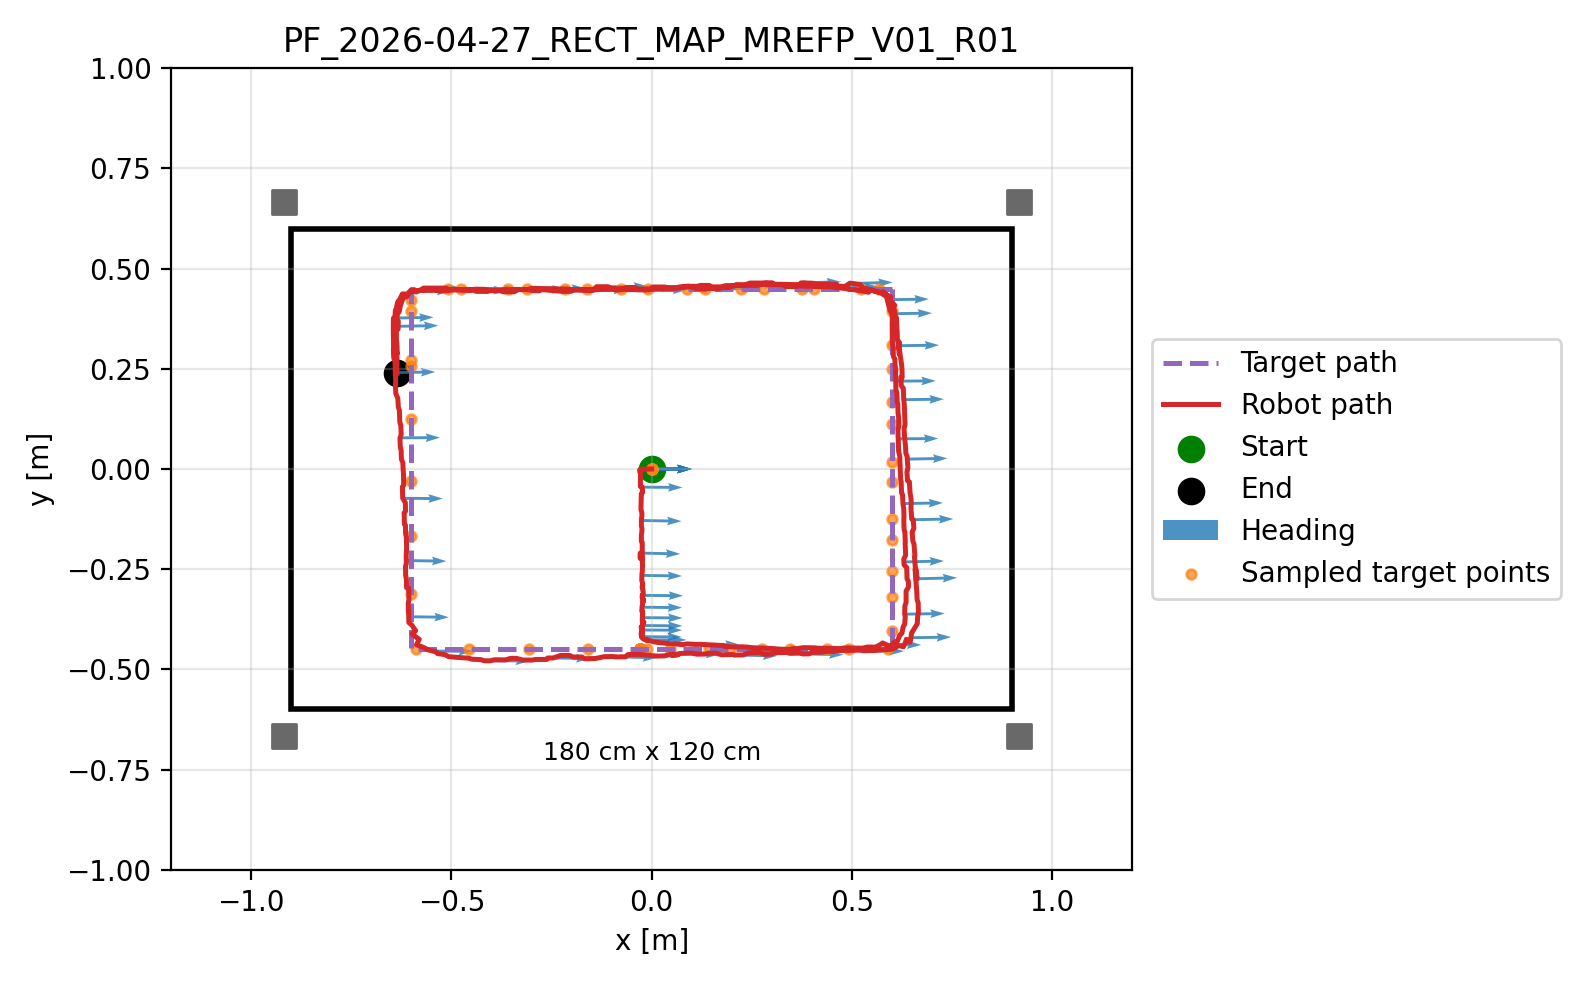
\includegraphics[width=0.7\linewidth]{IMG/controller/MREFP/MR_R01_xy_map.png}
        \caption{MR\_R01 xy map}
        \label{fig:MR_R01_xy_map}
    \end{subfigure}

    \vspace{0.2em}

    \begin{subfigure}{\textwidth}
        \centering
        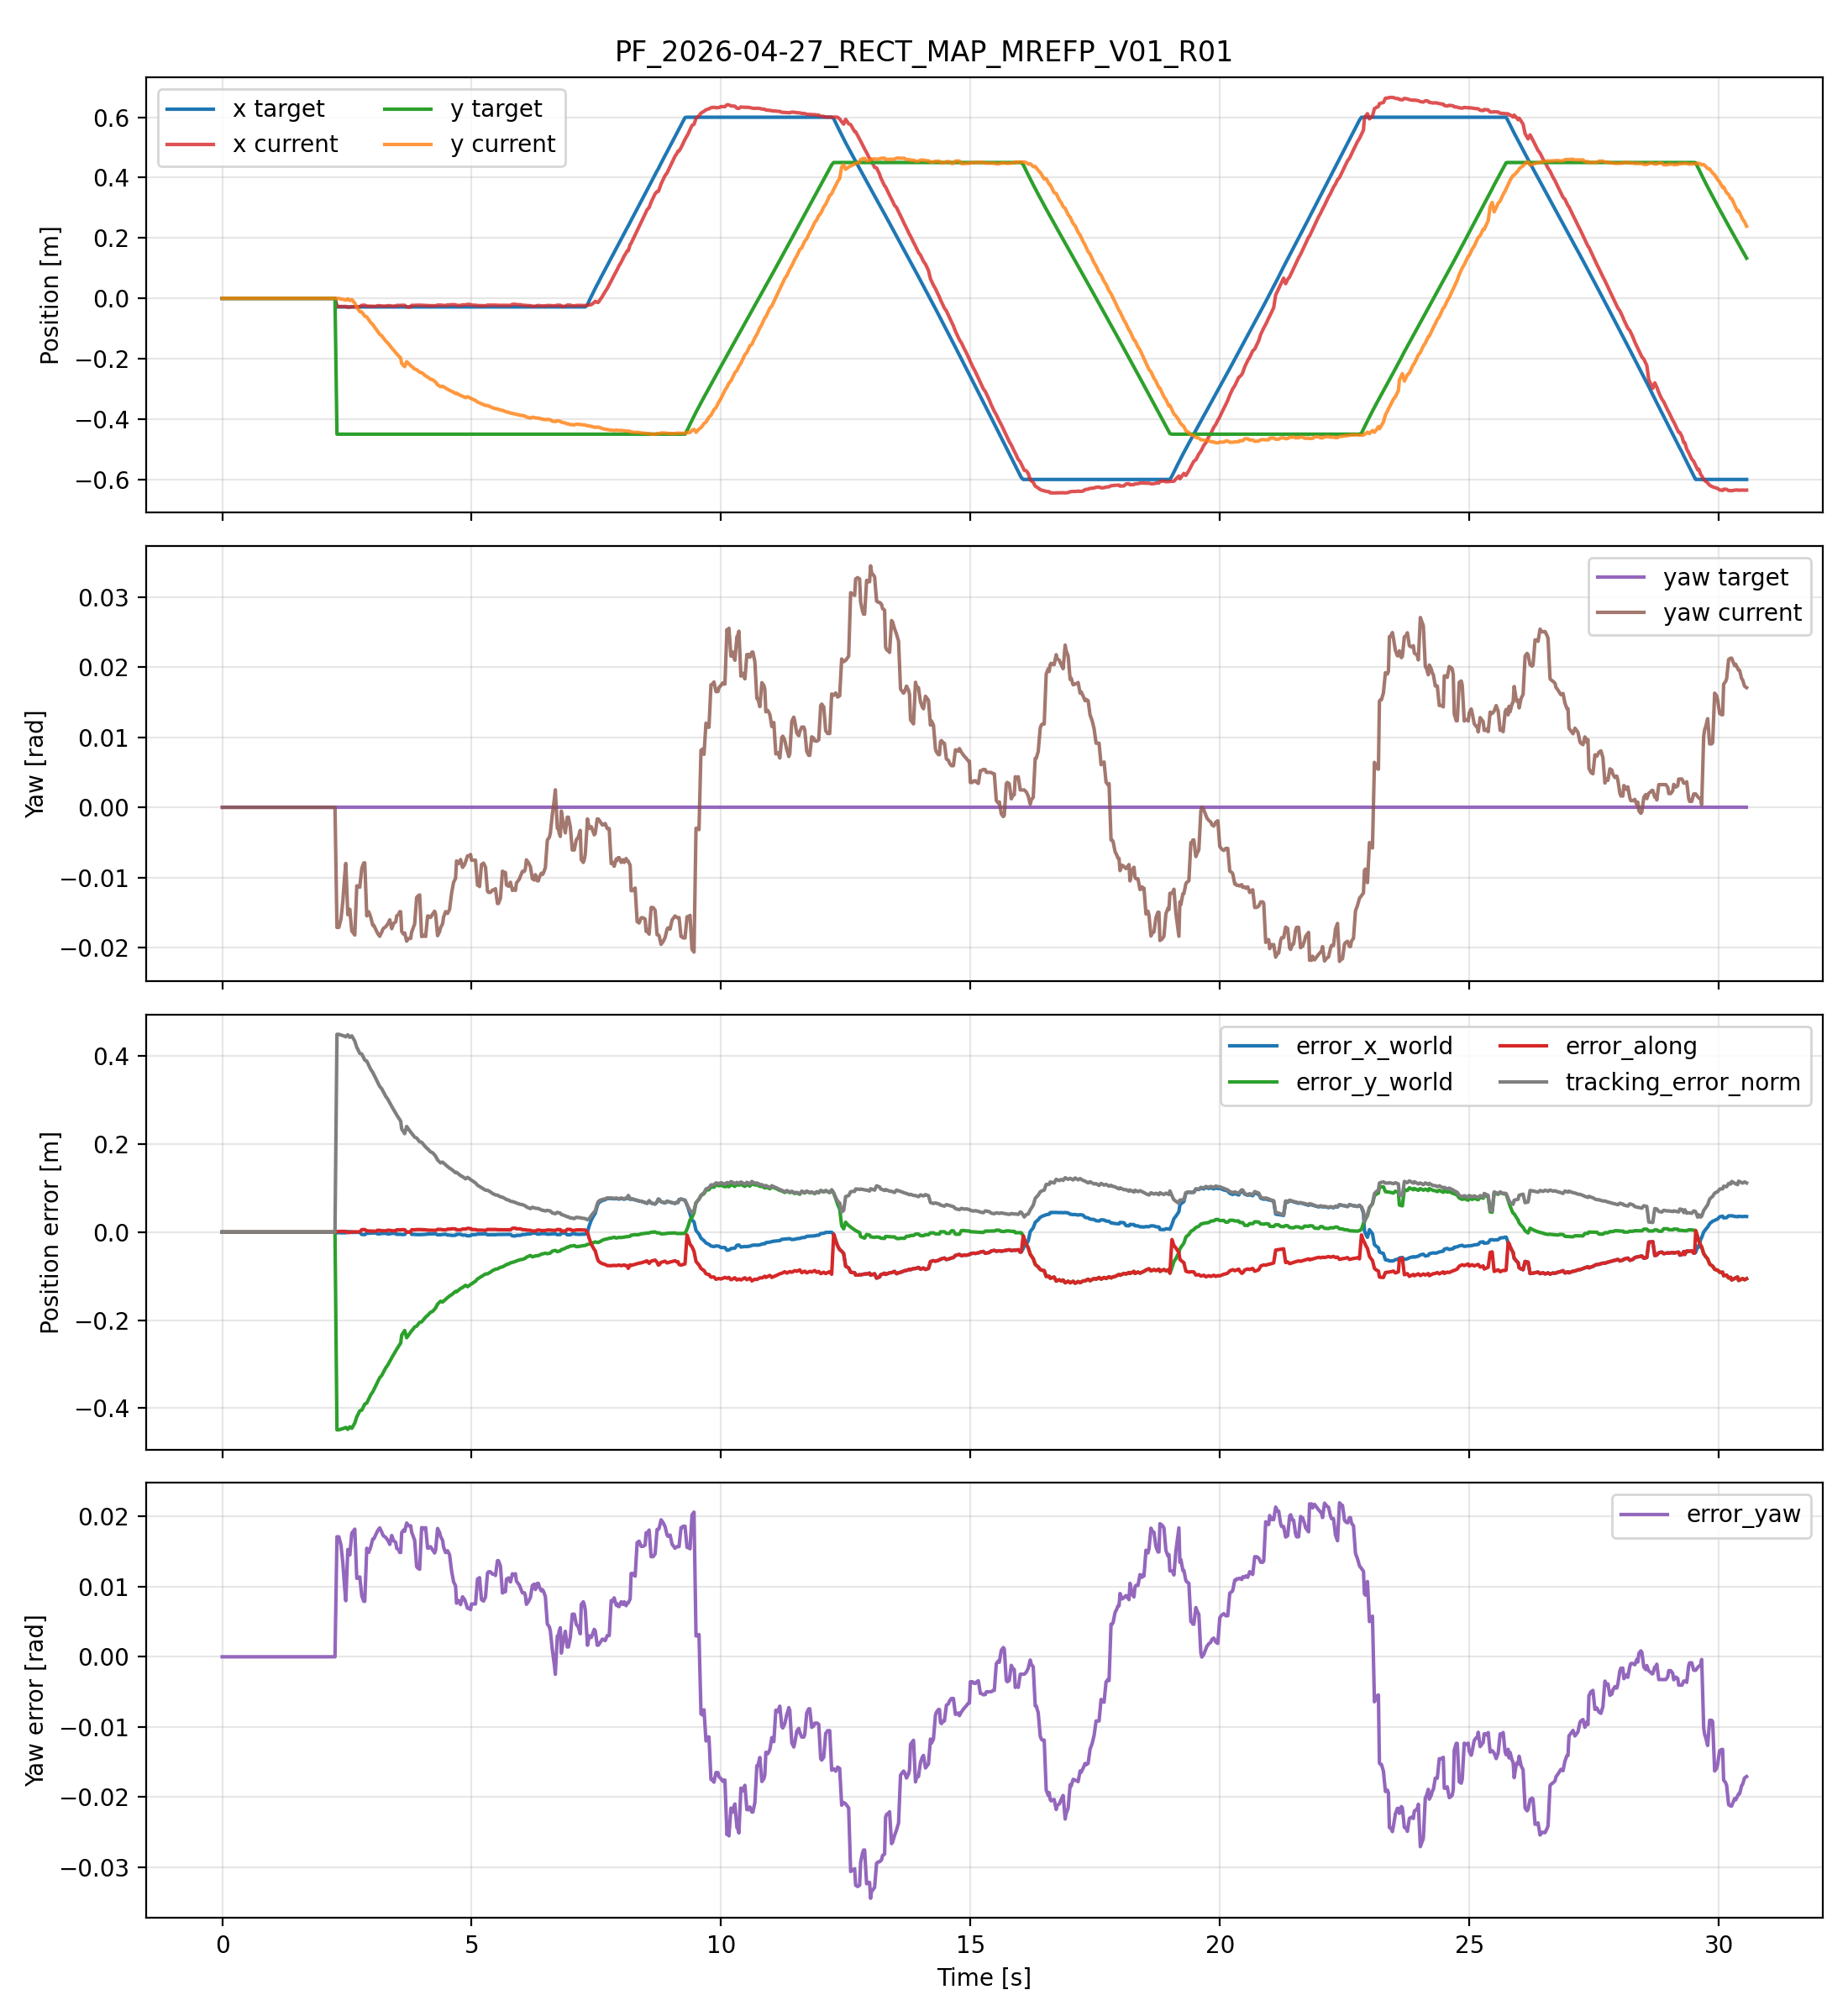
\includegraphics[width=0.6\linewidth]{IMG/controller/MREFP/MR_R01_target_tracking_and_errors.png}
        \caption{MR\_R01 tracking and errors}
        \label{fig:MR_R01_tracking_and_errors}
    \end{subfigure}
    
    \vspace{0.2em}
    \caption{Experimental results for MR\_R01 scenario.} 
    \label{fig:MR_R01_general}
\end{figure}

\newpage
\begin{figure}[H]
    \centering
    \begin{subfigure}{\textwidth}
        \centering
        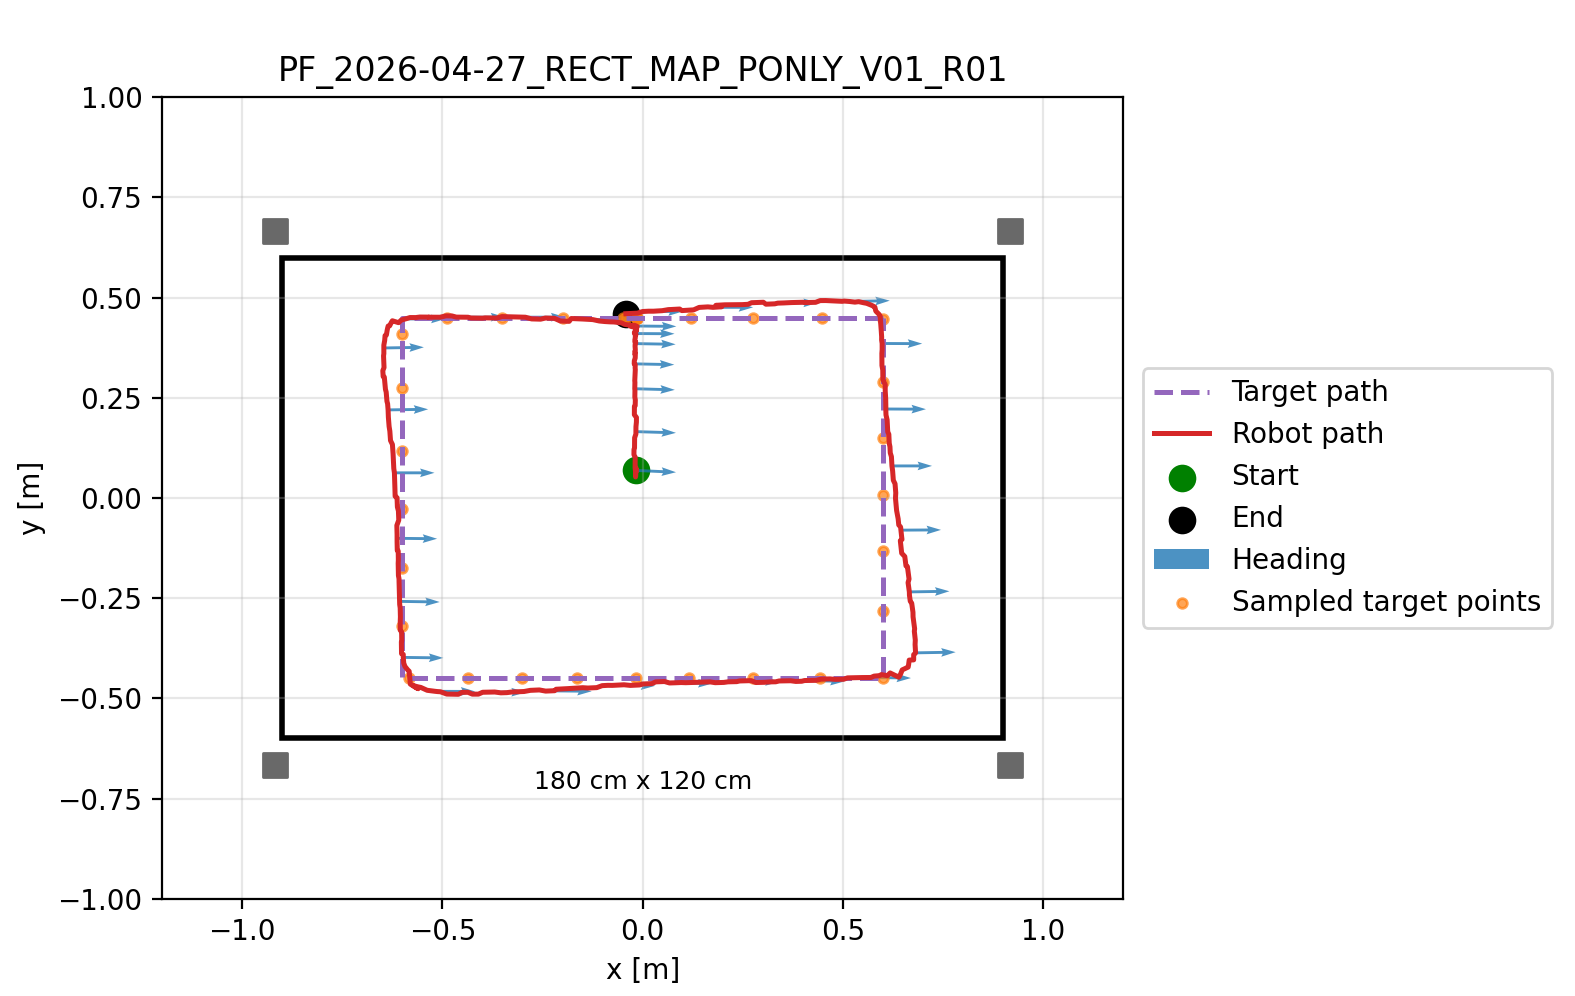
\includegraphics[width=0.7\linewidth]{IMG/controller/MREFP/PR01_xy_map.png}
        \caption{P\_R01 xy map}
        \label{fig:PR01_xy_map}
    \end{subfigure}

    \vspace{0.2em}

    \begin{subfigure}{\textwidth}
        \centering
        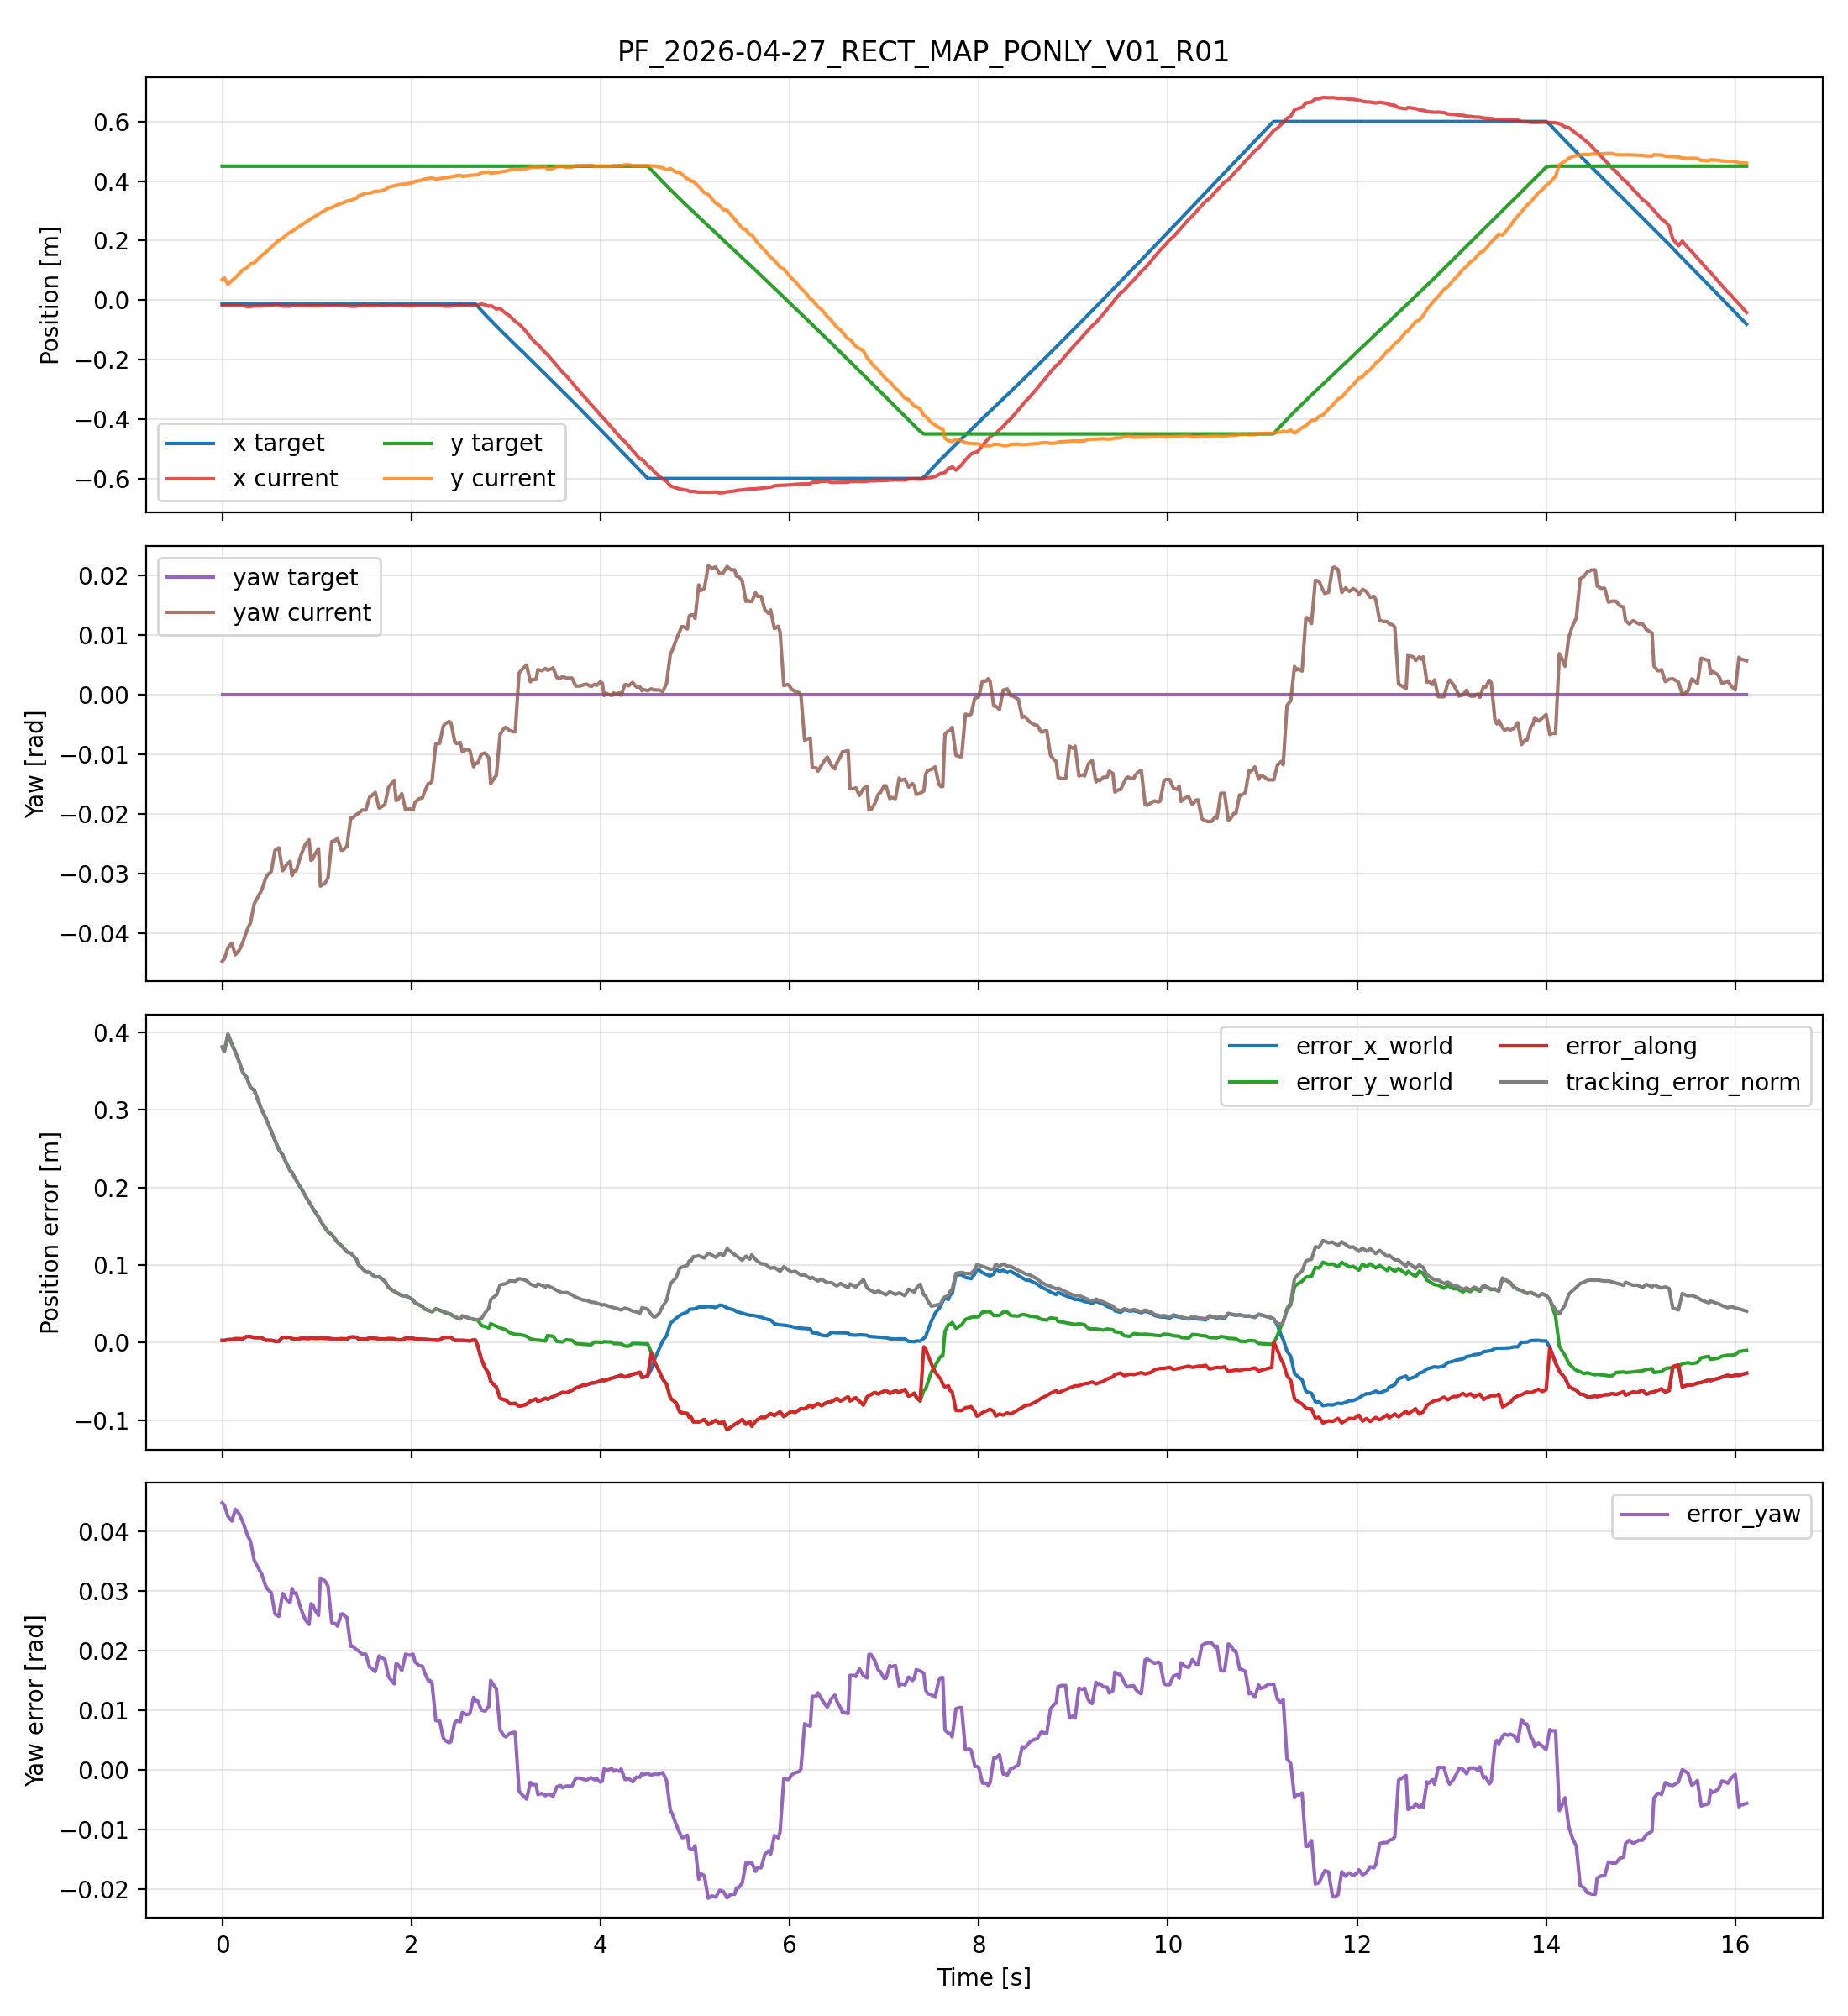
\includegraphics[width=0.7\linewidth]{IMG/controller/MREFP/PR01_target_tracking_and_errors.png}
        \caption{P\_R01 tracking and errors}
        \label{fig:PR01_tracking_and_errors}
    \end{subfigure}
    
    \vspace{0.2em}
    \caption{Experimental results for P\_R01 scenario.} 
    \label{fig:PR01_general}
\end{figure}

\newpage
\begin{figure}[H]
    \centering
    \begin{subfigure}{\textwidth}
        \centering
        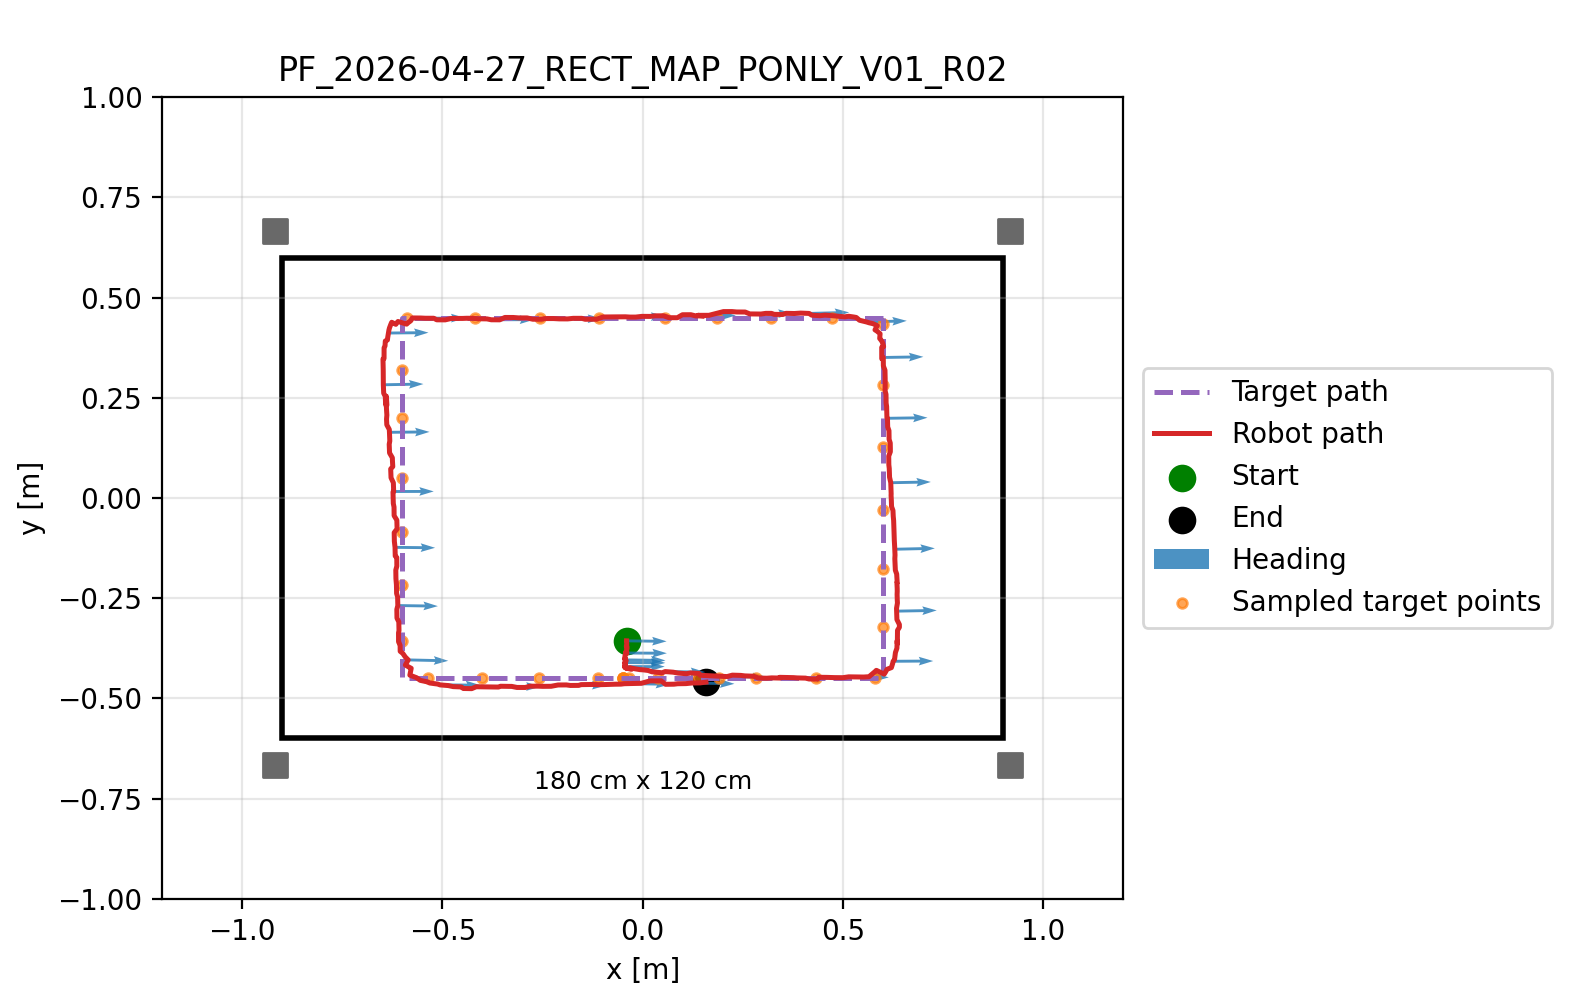
\includegraphics[width=0.7\linewidth]{IMG/controller/MREFP/PR02_xy_map.png}
        \caption{P\_R02 xy map}
        \label{fig:PR02_xy_map}
    \end{subfigure}

    \vspace{0.2em}

    \begin{subfigure}{\textwidth}
        \centering
        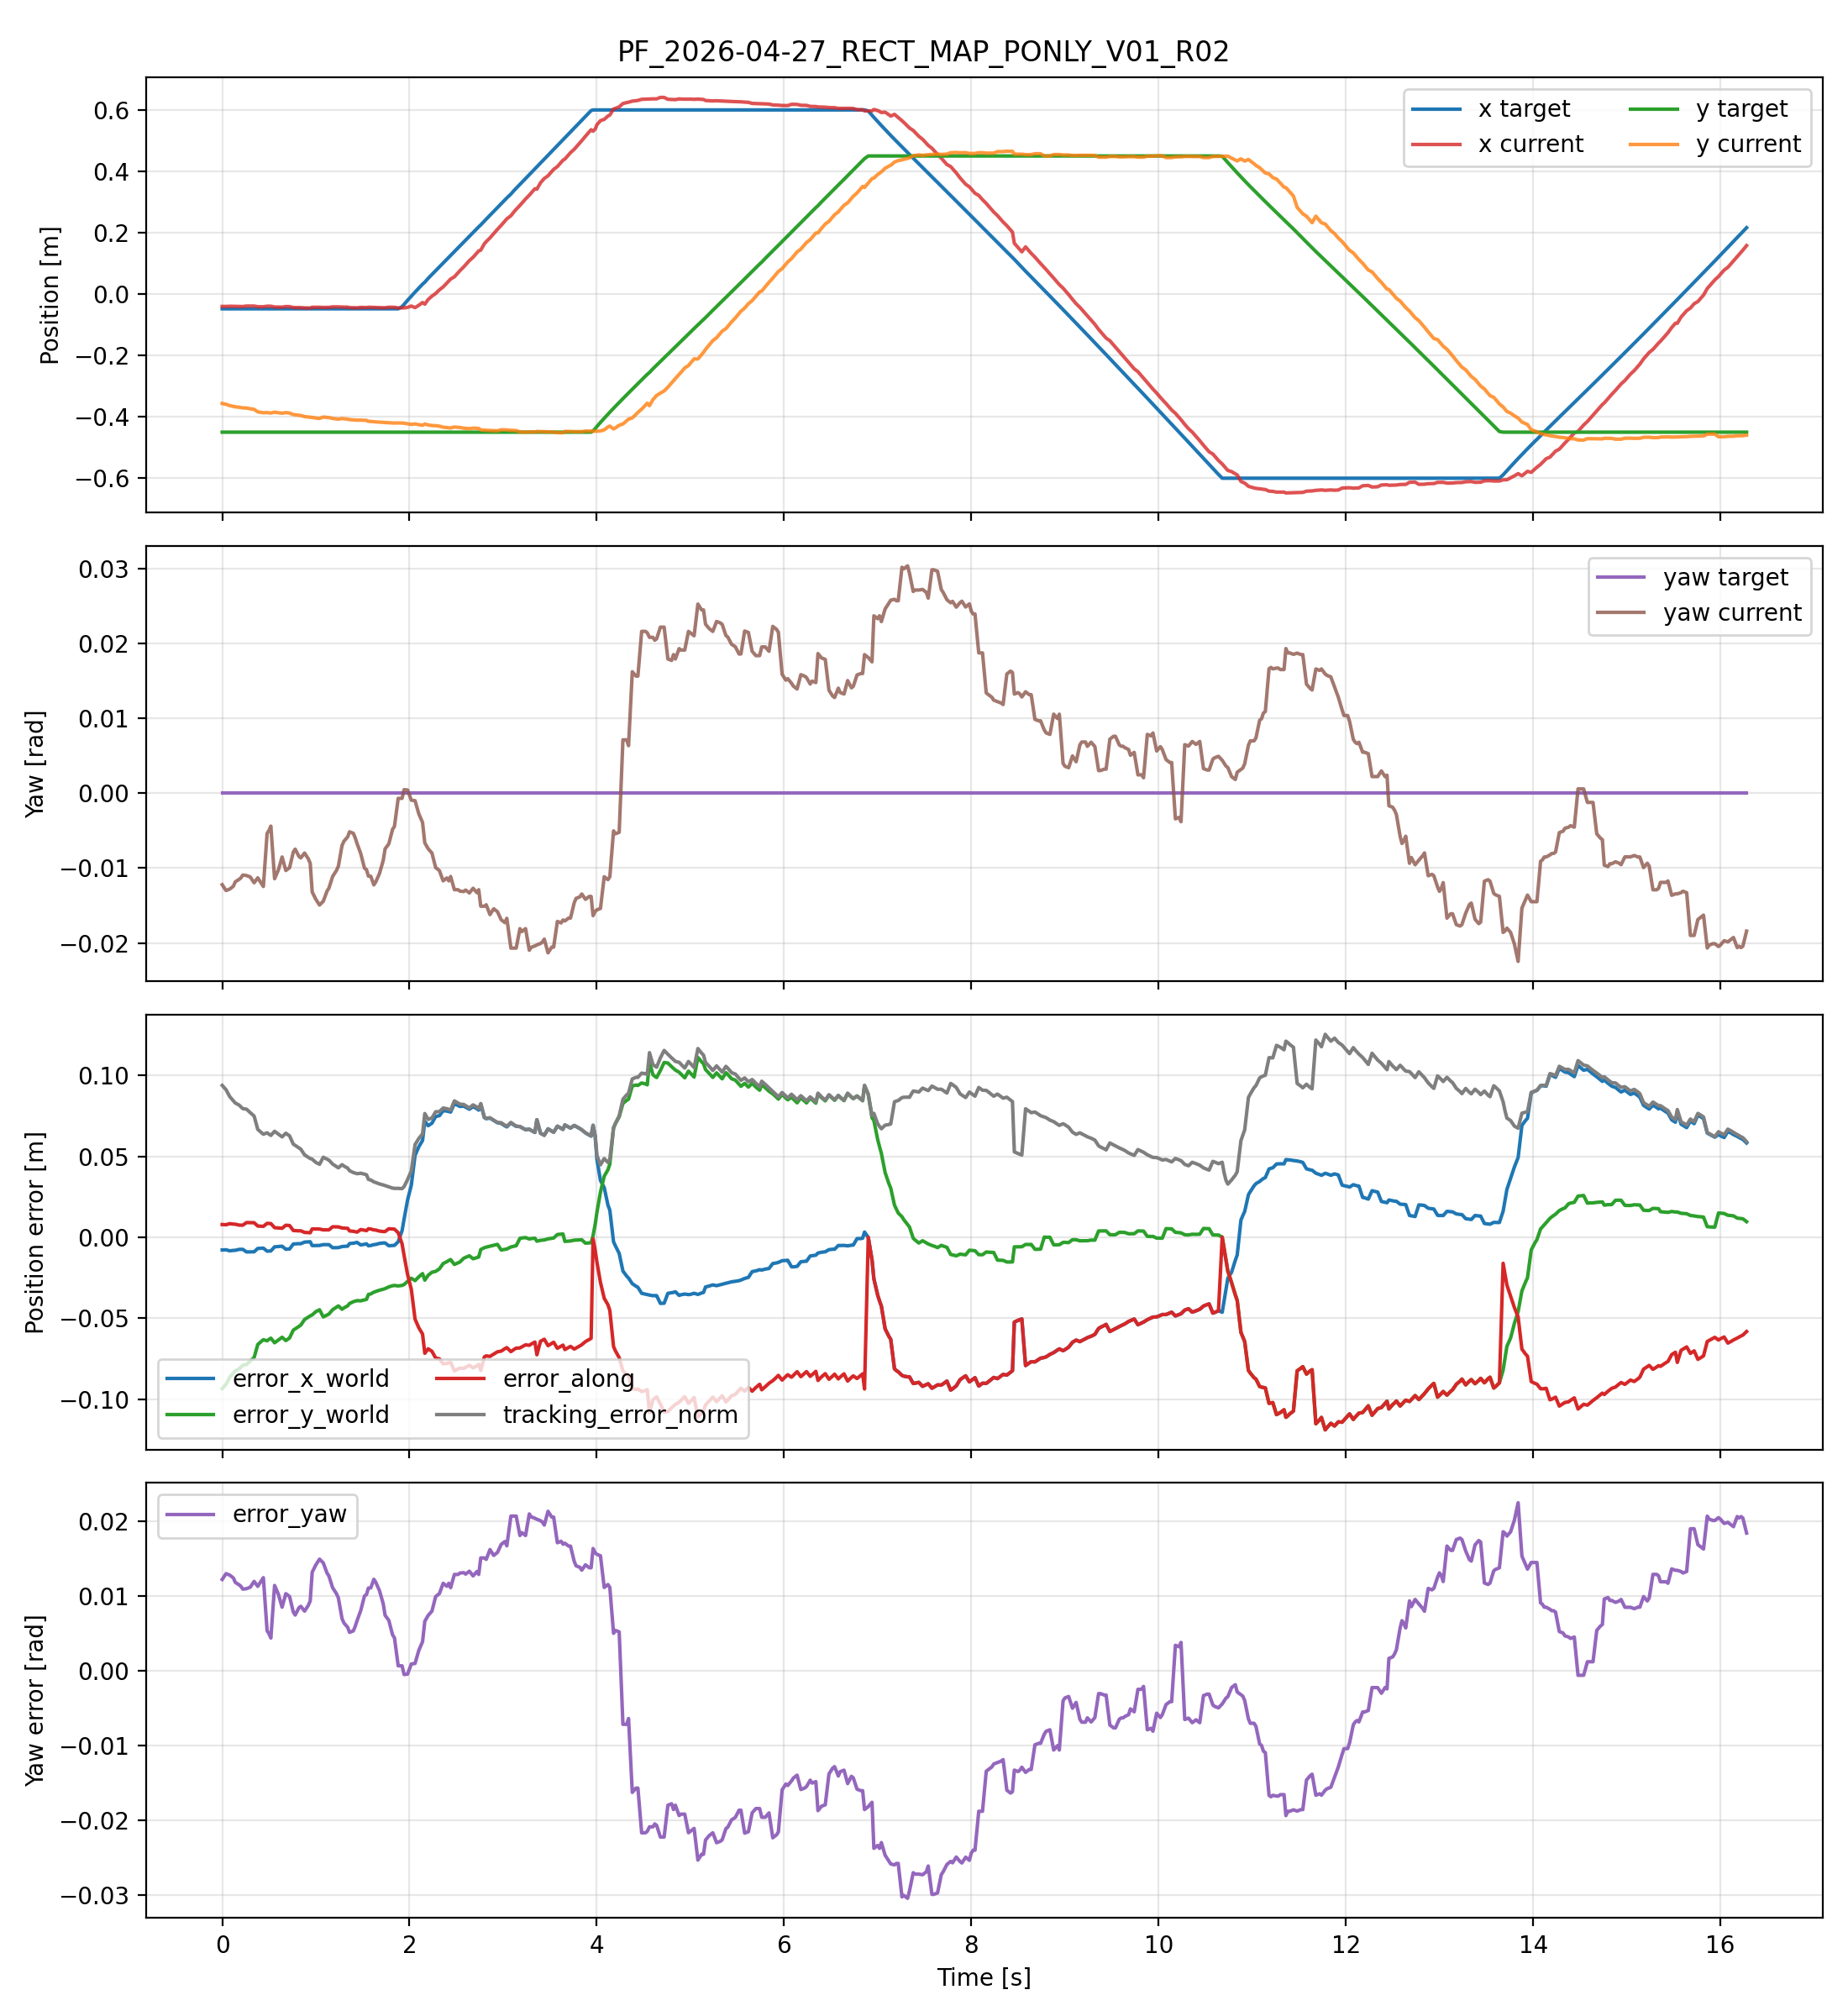
\includegraphics[width=0.7\linewidth]{IMG/controller/MREFP/PR02_target_tracking_and_errors.png}
        \caption{P\_R02 tracking and errors}
        \label{fig:PR02_tracking_and_errors}
    \end{subfigure}
    
    \vspace{0.2em}
    \caption{Experimental results for P\_R02 scenario.} 
    \label{fig:PR01_general}
\end{figure}

\section{Linear Segment Controller}
\subsection{Control Principle}

The Linear Segment controller uses the local geometry of the path. At each
control step, the robot position is projected onto the current path segment.
Given two consecutive path points:
\begin{equation}
    \mathbf{p}_i
    =
    \begin{bmatrix}
        x_i \\
        y_i
    \end{bmatrix},
    \qquad
    \mathbf{p}_{i+1}
    =
    \begin{bmatrix}
        x_{i+1} \\
        y_{i+1}
    \end{bmatrix},
\end{equation}
the segment vector is:
\begin{equation}
    \mathbf{s}_i
    =
    \mathbf{p}_{i+1}
    -
    \mathbf{p}_i.
\end{equation}

The unit tangent vector is:
\begin{equation}
    \mathbf{t}_i
    =
    \frac{\mathbf{s}_i}{\|\mathbf{s}_i\|}.
\end{equation}

The normal vector is obtained by rotating the tangent by \(90^\circ\):
\begin{equation}
    \mathbf{n}_i
    =
    \begin{bmatrix}
        -t_{i,y} \\
        t_{i,x}
    \end{bmatrix}.
\end{equation}

The projection coefficient is:
\begin{equation}
    \alpha
    =
    \frac{
        (\mathbf{p} - \mathbf{p}_i)^T \mathbf{s}_i
    }{
        \mathbf{s}_i^T \mathbf{s}_i
    }.
\end{equation}

To keep the projected point inside the segment, \(\alpha\) is limited:
\begin{equation}
    \alpha_c
    =
    \mathrm{sat}(\alpha,0,1).
\end{equation}

The closest point on the segment is:
\begin{equation}
    \mathbf{p}_{c}
    =
    \mathbf{p}_i
    +
    \alpha_c \mathbf{s}_i.
\end{equation}

The position error is:
\begin{equation}
    \mathbf{e}
    =
    \mathbf{p}_{c}
    -
    \mathbf{p}.
\end{equation}

This error is decomposed into an along-track component and a lateral component:
\begin{equation}
    e_{\parallel}
    =
    \mathbf{e}^{T}\mathbf{t}_i,
    \qquad
    e_{\perp}
    =
    \mathbf{e}^{T}\mathbf{n}_i.
\end{equation}

The desired velocity in the world frame is:
\begin{equation}
    \mathbf{v}_{w}
    =
    v_d \mathbf{t}_i
    +
    k_{\parallel} e_{\parallel} \mathbf{t}_i
    +
    k_{\perp} e_{\perp} \mathbf{n}_i.
\end{equation}

The first term moves the robot along the path. The second term corrects the
longitudinal error. The third term corrects the lateral error and is the main
term used to reduce the cross-track deviation.

Since the robot command is expressed in body frame, the world-frame velocity is
rotated using:
\begin{equation}
    \mathbf{v}_{b}
    =
    \mathbf{R}^{T}(\psi)
    \mathbf{v}_{w}.
\end{equation}

Therefore:
\begin{equation}
    v_x = v_{b,x},
    \qquad
    v_y = v_{b,y}.
\end{equation}

The yaw motion is controlled separately:
\begin{equation}
    \omega
    =
    k_{\psi}
    \mathrm{wrapToPi}(\psi_r - \psi).
\end{equation}

This formulation is useful for an omnidirectional robot because longitudinal
motion and lateral correction can be commanded at the same time. For this
reason, the robot does not need to align its body with the path before reducing
the lateral error.

\subsection{Test Parameters}

\noindent
  \textbf{Test legend:}
  \begin{itemize}
      \item \textbf{LIN-01}: \texttt{PF\_2026-04-28\_INFIN\_MAP\_LINEAR\_V01\_R01};
      \item \textbf{LIN-02}: \texttt{PF\_2026-04-29\_INFIN\_MAP\_LINEAR\_V01\_R02};
      \item \textbf{LIN-03}: \texttt{PF\_2026-04-29\_INFIN\_MAP\_LINEAR\_V01\_R07};
      \item \textbf{LIN-04}: \texttt{PF\_2026-04-29\_INFIN\_MAP\_LINEAR\_V01\_R08};
      \item \textbf{LIN-05}: \texttt{PF\_2026-04-29\_INFIN\_MAP\_LINEAR\_V01\_R10}.
  \end{itemize}

  \begin{table}[H]
  \centering
  \caption{Linear Segment controller: configuration parameters of the selected tests.}
  \label{tab:linear_configuration_parameters}
  \small
  \begin{tabular}{lccccc}
  \toprule
  \textbf{Parameter} &
  \textbf{LIN-01} &
  \textbf{LIN-02} &
  \textbf{LIN-03} &
  \textbf{LIN-04} &
  \textbf{LIN-05} \\
  \midrule
  Path & INFIN & INFIN & INFIN & INFIN & INFIN \\
  Frame & MAP & MAP & MAP & MAP & MAP \\
  Heading mode & fixed & fixed & fixed & fixed & fixed \\
  \(v_d\) [m/s] & 0.35 & 0.20 & 0.30 & 0.40 & 0.50 \\
  \(k_{\gamma}\) & 0.20 & 0.20 & 0.20 & 0.30 & 0.40 \\
  \(\dot{\gamma}_{\min}\) [m/s] & 0.10 & 0.05 & 0.05 & 0.05 & 0.05 \\
  \(\dot{\gamma}_{\max}\) [m/s] & 0.35 & 0.20 & 0.20 & 0.30 & 0.30 \\
  \(k_{\parallel}\) & 0.00 & 0.40 & 1.00 & 1.00 & 1.00 \\
  \(k_{\perp}\) & 0.80 & 3.00 & 5.00 & 5.00 & 8.00 \\
  Control rate [Hz] & 50 & 50 & 50 & 50 & 50 \\
  \bottomrule
  \end{tabular}
  \end{table}

  \begin{table}[H]
  \centering
  \caption{Linear Segment controller: experimental results of the selected tests.}
  \label{tab:linear_experimental_results}
  \small
  \begin{tabular}{lccccc}
  \toprule
  \textbf{Metric} &
  \textbf{LIN-01} &
  \textbf{LIN-02} &
  \textbf{LIN-03} &
  \textbf{LIN-04} &
  \textbf{LIN-05} \\
  \midrule
  Duration [s] & 23.80 & 39.20 & 32.28 & 27.39 & 22.58 \\
  Samples & 753 & 1268 & 1020 & 853 & 716 \\
  Mean sample time [s] & 0.0316 & 0.0309 & 0.0317 & 0.0321 & 0.0316 \\
  Real path length [m] & 7.7631 & 7.7922 & 9.6978 & 10.7535 & 11.6237 \\
  Final \(\gamma\) [m] & 2.0687 & 4.4860 & 2.0970 & 2.1181 & 2.1832 \\
  Path progress ratio \(r_{\gamma}\) & 0.4542 & 0.9849 & 0.4604 & 0.4650 & 0.4793 \\
  \(\mathrm{RMSE}_x\) [m] & 0.0720 & 0.0125 & 0.0172 & 0.0270 & 0.0396 \\
  \(\mathrm{RMSE}_y\) [m] & 0.0586 & 0.0113 & 0.0148 & 0.0228 & 0.0252 \\
  \(\mathrm{RMSE}_{\psi}\) [rad] & 0.0139 & 0.0082 & 0.0120 & 0.0187 & 0.0324 \\
  \(\mathrm{RMSE}_{e_{\parallel}}\) [m] & 0.0028 & 0.0003 & 0.0005 & 0.0005 & 0.0009 \\
  \(\mathrm{MAE}_{e_{\parallel}}\) [m] & 0.0009 & 0.00005 & 0.00008 & 0.00010 & 0.00020 \\
  \(\max |e_{\parallel}|\) [m] & 0.0217 & 0.0037 & 0.0049 & 0.0057 & 0.0104 \\
  \(\mathrm{IAE}_{e_{\parallel}}\) & 0.0206 & 0.0020 & 0.0025 & 0.0027 & 0.0044 \\
  \(\max |e_{\psi}|\) [rad] & 0.0340 & 0.0264 & 0.0310 & 0.0464 & 0.0745 \\
  Saturation ratio \(v_x\) & 0.0000 & 0.0000 & 0.0186 & 0.0668 & 0.2304 \\
  Saturation ratio \(v_y\) & 0.0000 & 0.0000 & 0.0461 & 0.0961 & 0.1955 \\
  Saturation ratio \(\omega\) & 0.0000 & 0.0000 & 0.0000 & 0.0000 & 0.0000 \\
  \bottomrule
  \end{tabular}
  \end{table}

 The experimental validation analyzes the impact of varying desired speeds ($v_d$) and feedback gains ($k_{\parallel}, k_{\perp}$) on the Linear Segment controller. All tests were conducted on an "infinity" path within the MAP frame, utilizing a fixed-heading mode. The primary objective is to evaluate the trade-off between path progression, tracking accuracy, and control effort.

\paragraph{Baseline and Tuning Impact (LIN-01)}
The baseline configuration, \textbf{LIN-01} ($v_d = 0.35~\mathrm{m/s}$), employs a weak feedback action with $k_{\parallel}=0$ and $k_{\perp}=0.8$. This setup results in the poorest tracking performance among the selected runs:
\[
    \mathrm{RMSE}_x = 0.0720~\mathrm{m}, \quad \mathrm{RMSE}_y = 0.0586~\mathrm{m}, \quad \mathrm{RMSE}_{e_{\parallel}} = 0.0028~\mathrm{m}
\]
Since saturation ratios remain at zero, the high tracking error is not due to physical actuator limits but is directly attributable to the insufficient feedback gains, particularly the absence of longitudinal compensation ($k_{\parallel}=0$).

\paragraph{Optimal Performance (LIN-02)}
The most balanced results are achieved in \textbf{LIN-02}. By reducing the speed to $v_d = 0.20~\mathrm{m/s}$ and increasing the gains to $k_{\parallel}=0.4$ and $k_{\perp}=3.0$, the tracking errors decrease significantly:
\[
    \mathrm{RMSE}_x = 0.0125~\mathrm{m}, \quad \mathrm{RMSE}_y = 0.0113~\mathrm{m}, \quad \mathrm{RMSE}_{e_{\parallel}} = 0.0003~\mathrm{m}
\]
This configuration provides high path completion and negligible error without encountering velocity saturation, establishing a robust benchmark for reliable autonomous navigation.

\paragraph{High-Speed Scenarios and Actuator Limits (LIN-03 to LIN-05)}
As the desired speed increases, a clear degradation in performance and an increase in control effort are observed:

\begin{itemize}
    \item \textbf{LIN-03 ($v_d = 0.30~\mathrm{m/s}$):} Despite maintaining good local accuracy, the path progress ratio drops to $r_{\gamma} = 0.4604$. The controller begins to approach the actuation limits, with saturation ratios reaching $1.86\%$ on $v_x$ and $4.61\%$ on $v_y$.
    \item \textbf{LIN-04 ($v_d = 0.40~\mathrm{m/s}$):} The system nears its operational limits. Position errors and heading divergence increase ($\mathrm{RMSE}_{\psi} = 0.0187~\mathrm{rad}$), while saturation becomes more frequent ($r_{\mathrm{sat},v_y} \approx 9.61\%$).
    \item \textbf{LIN-05 ($v_d = 0.50~\mathrm{m/s}$):} In the fastest test, the controller hits significant saturation ($\approx 23\%$ on $v_x$). This prevents the full application of corrective commands, leading to the highest observed errors:
    \[
        \mathrm{RMSE}_x = 0.0396~\mathrm{m}, \quad \max |e_{\psi}| = 0.0745~\mathrm{rad}
    \]
\end{itemize}


\paragraph{Concluding Remarks}
The results demonstrate a direct correlation between target velocity and tracking stability. While \textbf{LIN-02} represents the ideal operational point for the current tuning, the high-speed tests highlight the physical and algorithmic boundaries of the system. To maintain accuracy at higher velocities, future developments should consider adaptive path progression or the introduction of feedforward terms to mitigate the lag induced by high-gain feedback during saturation.

\newpage
\begin{figure}[H]
    \centering
    \begin{subfigure}{\textwidth}
        \centering
        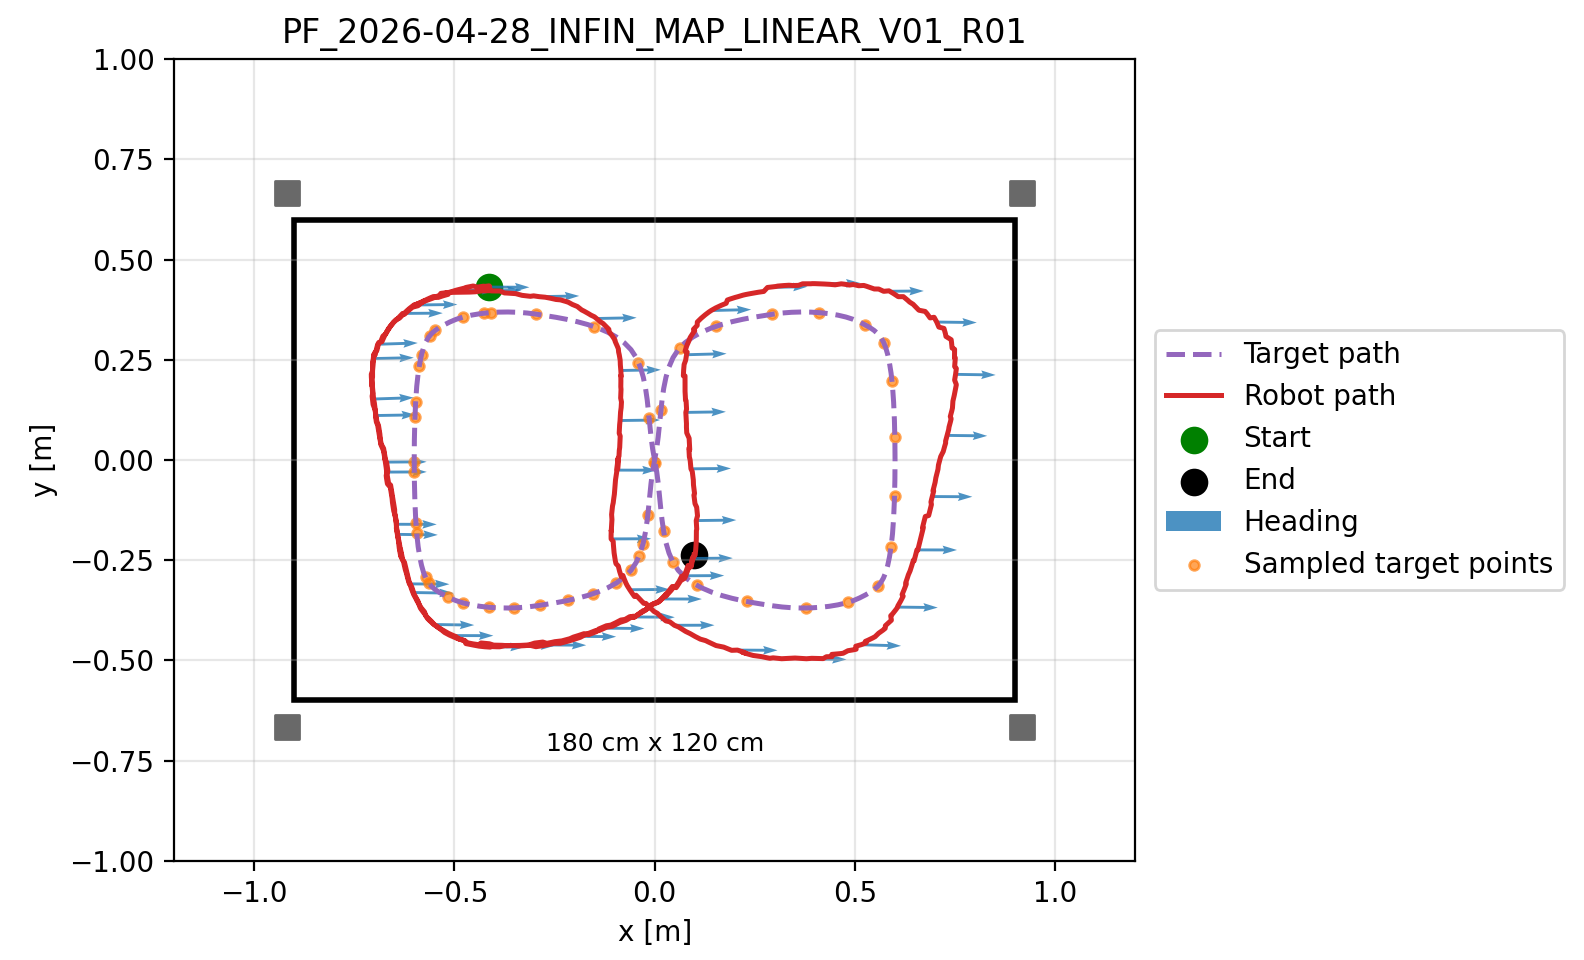
\includegraphics[width=0.7\linewidth]{IMG/controller/LIN/LIN_01_xy_map.png}
        \caption{LIN\_01 xy map}
        \label{fig:LIN_01_xy_map}
    \end{subfigure}

    \vspace{0.5em}

    \begin{subfigure}{\textwidth}
        \centering
        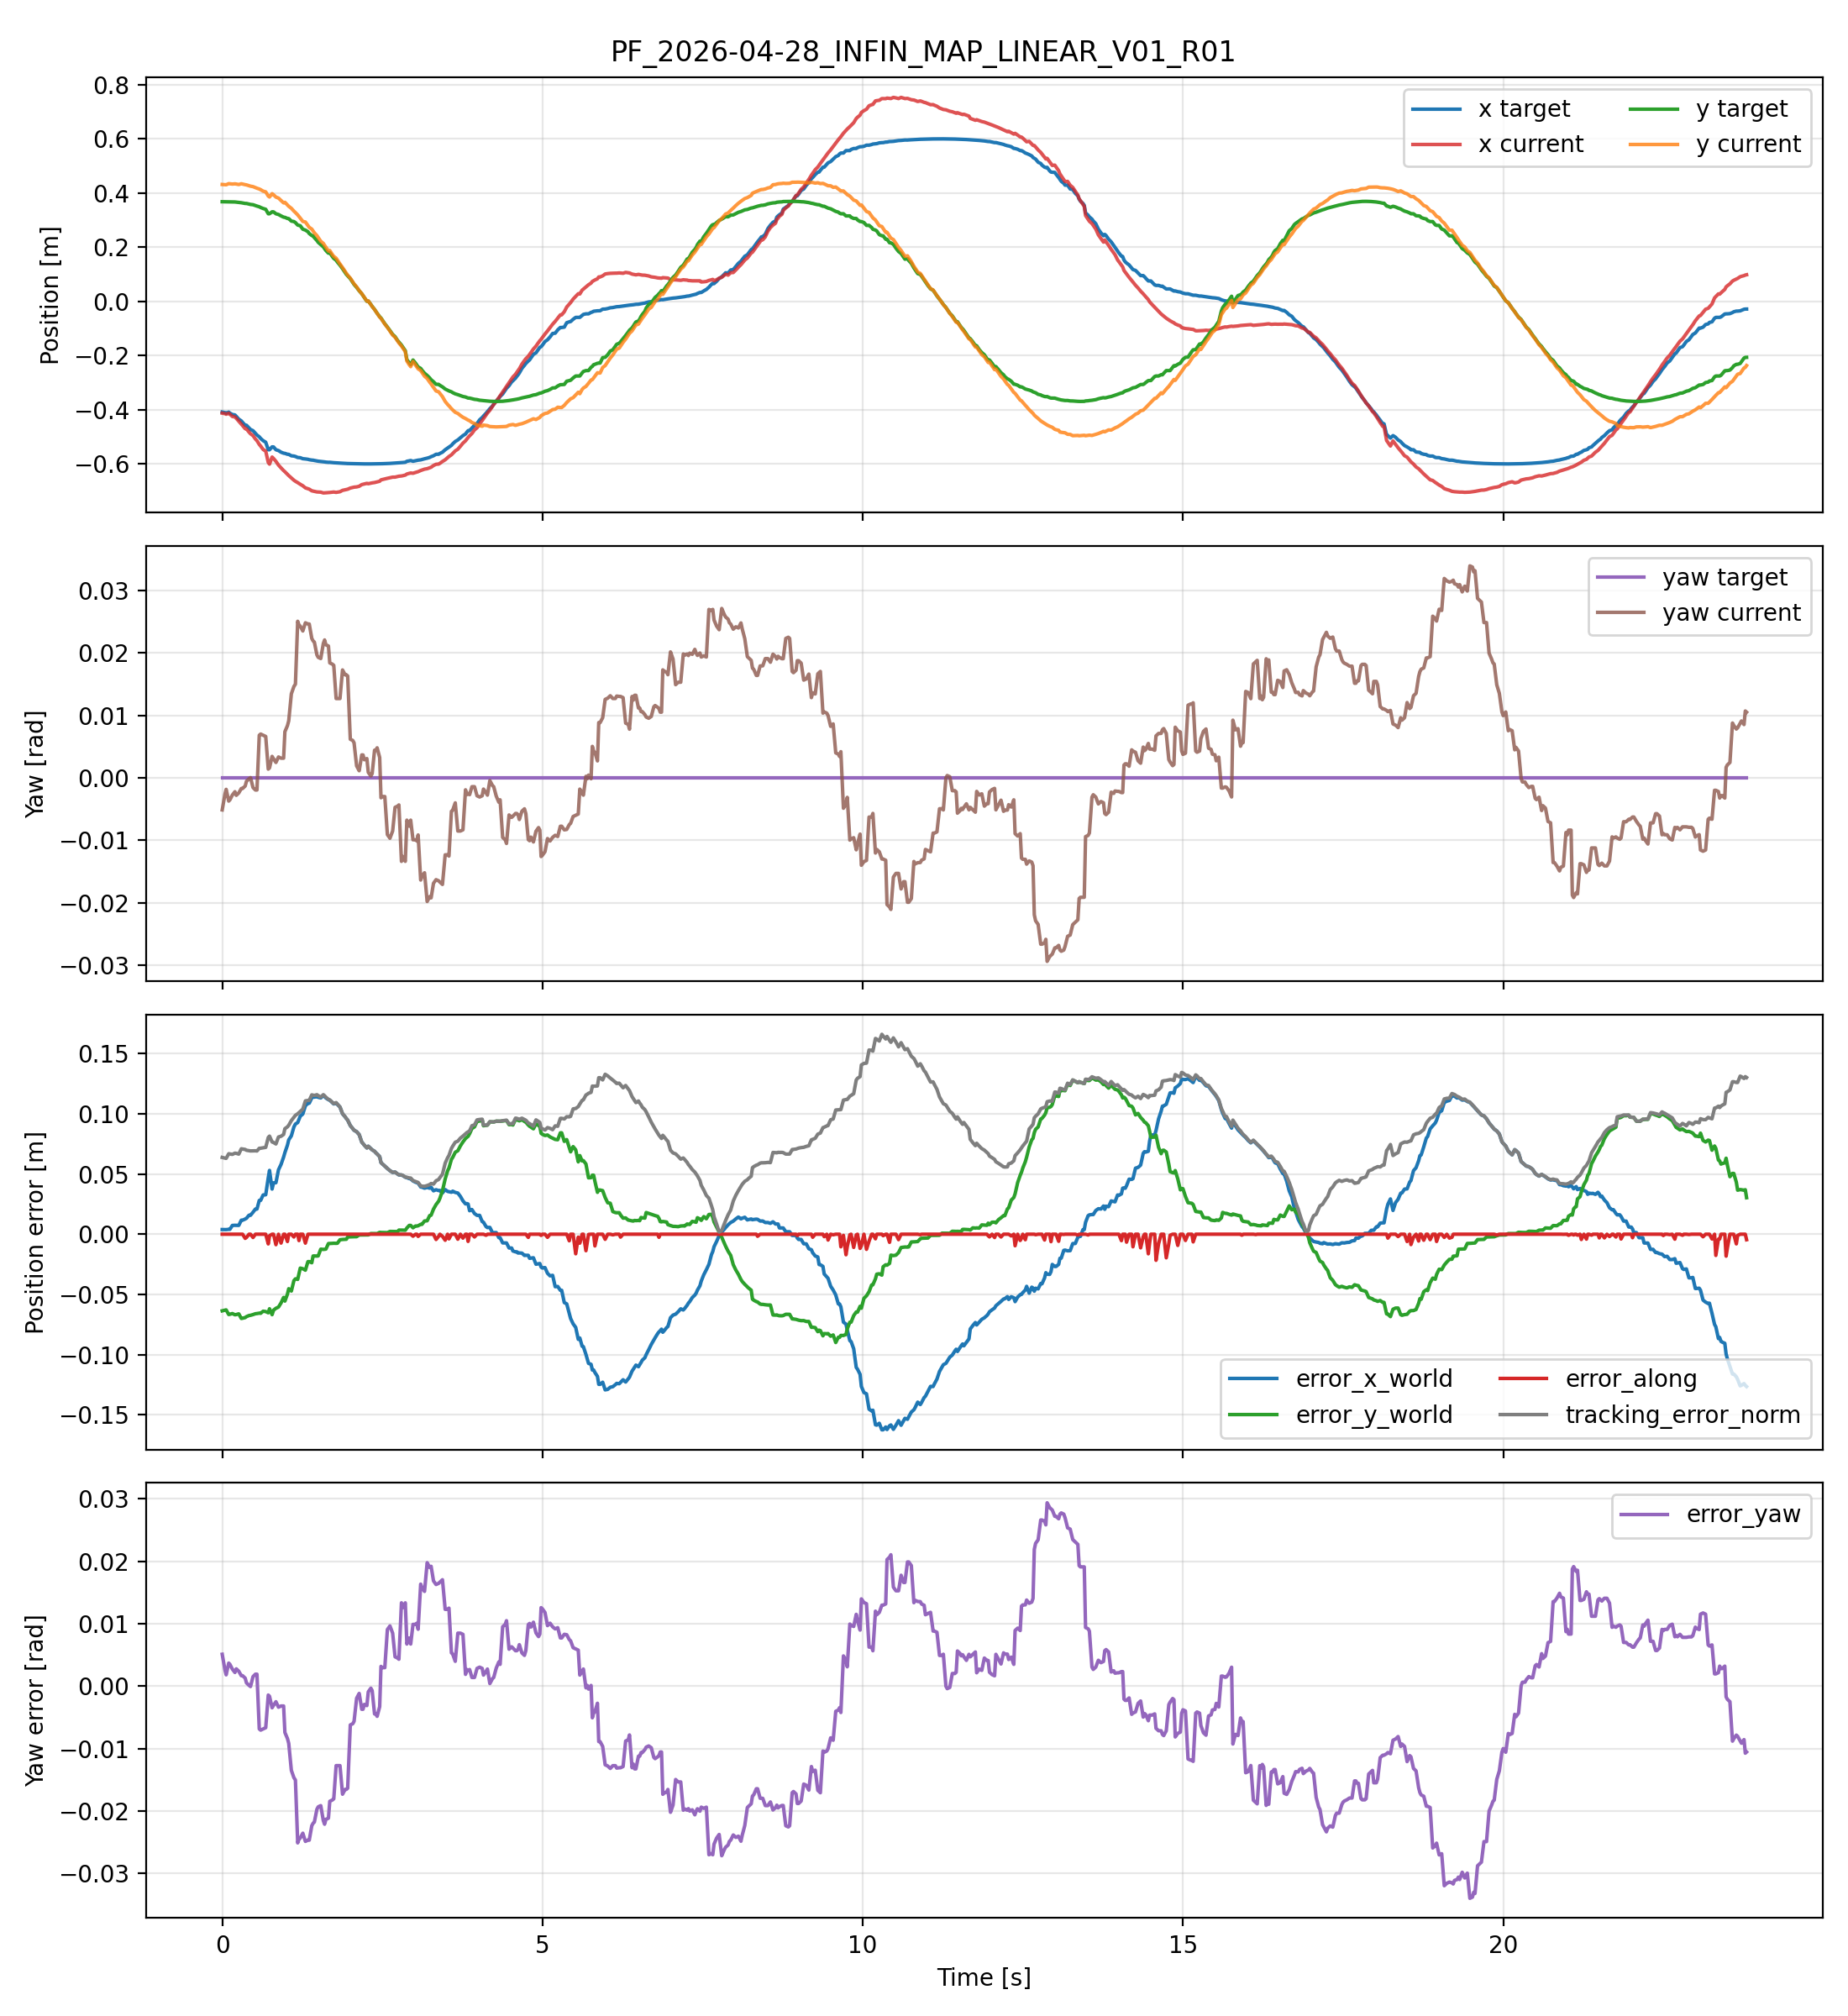
\includegraphics[width=0.7\linewidth]{IMG/controller/LIN/LIN_01_target_tracking_and_errors.png}
        \caption{LIN\_01 tracking and errors}
        \label{fig:LIN_01_tracking_and_errors}
    \end{subfigure}
    
    \vspace{0.5em}
    \caption{Experimental results for LIN\_01 scenario.} 
    \label{fig:LIN_01_general}
\end{figure}

\newpage
\begin{figure}[H]
    \centering
    \begin{subfigure}{\textwidth}
        \centering
        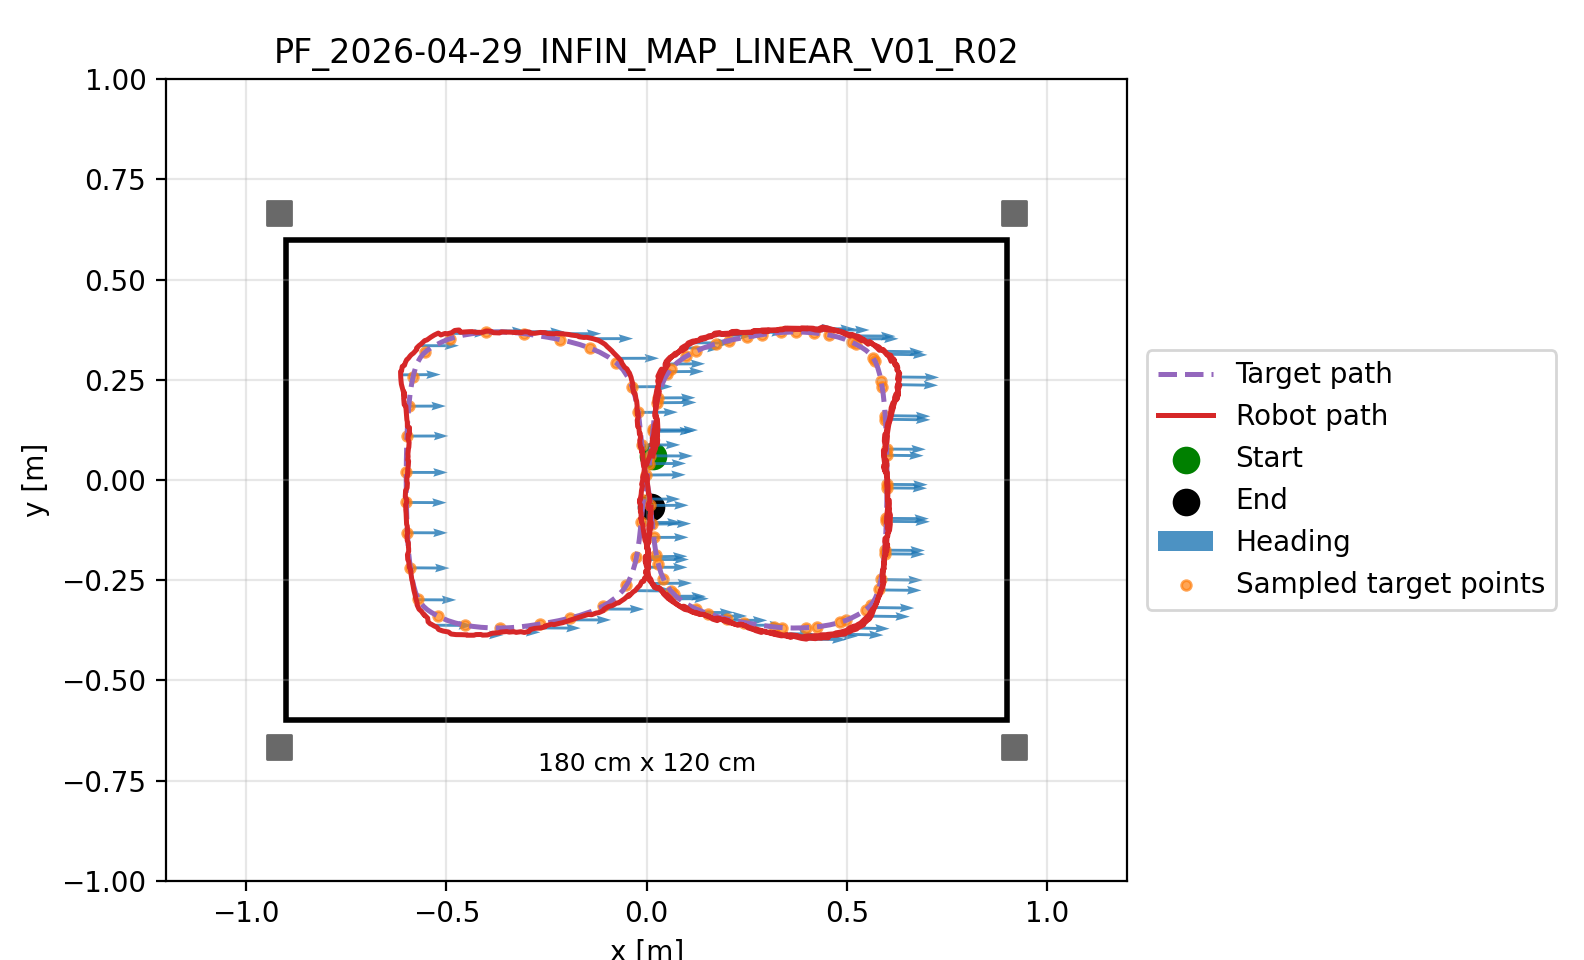
\includegraphics[width=0.7\linewidth]{IMG/controller/LIN/LIN_02_xy_map.png}
        \caption{LIN\_02 xy map}
        \label{fig:LIN_02_xy_map}
    \end{subfigure}

    \vspace{0.5em}

    \begin{subfigure}{\textwidth}
        \centering
        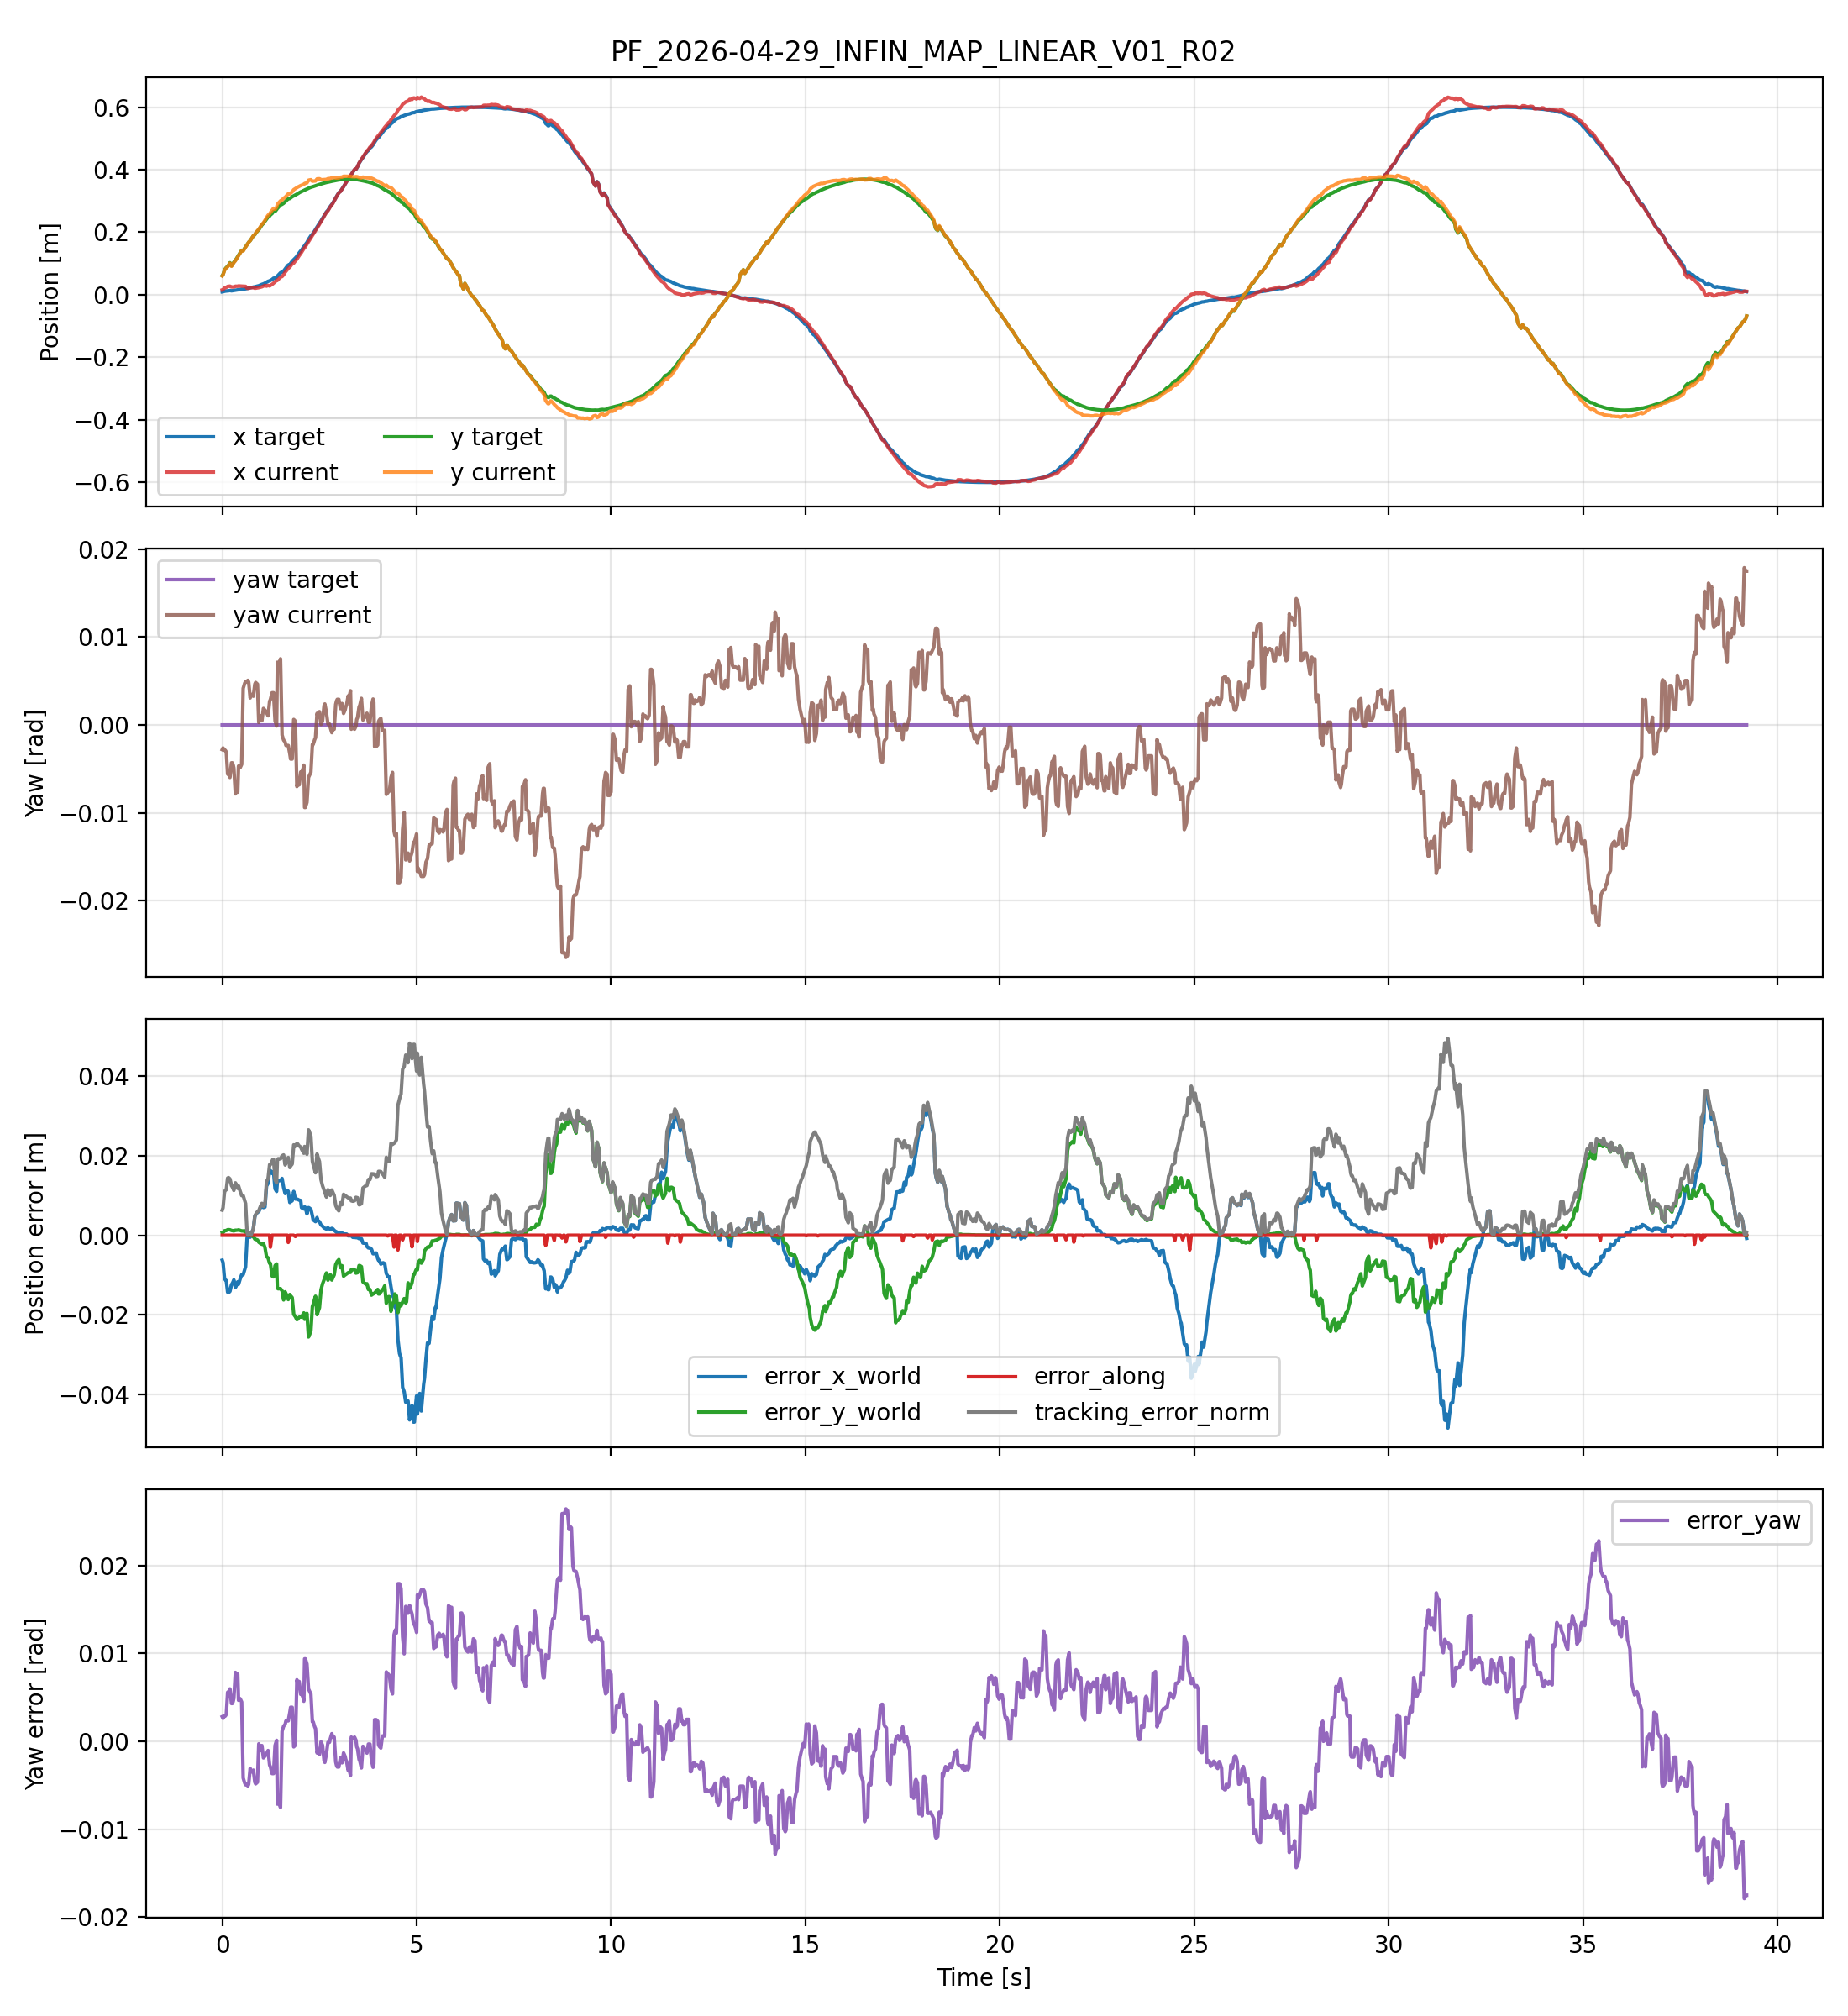
\includegraphics[width=0.7\linewidth]{IMG/controller/LIN/LIN_02_target_tracking_and_errors.png}
        \caption{LIN\_02 tracking and errors}
        \label{fig:LIN_02_tracking_and_errors}
    \end{subfigure}
    
    \vspace{0.5em}
    \caption{Experimental results for LIN\_02 scenario.} 
    \label{fig:LIN_02_general}
\end{figure}

\newpage
\begin{figure}[H]
    \centering
    \begin{subfigure}{\textwidth}
        \centering
        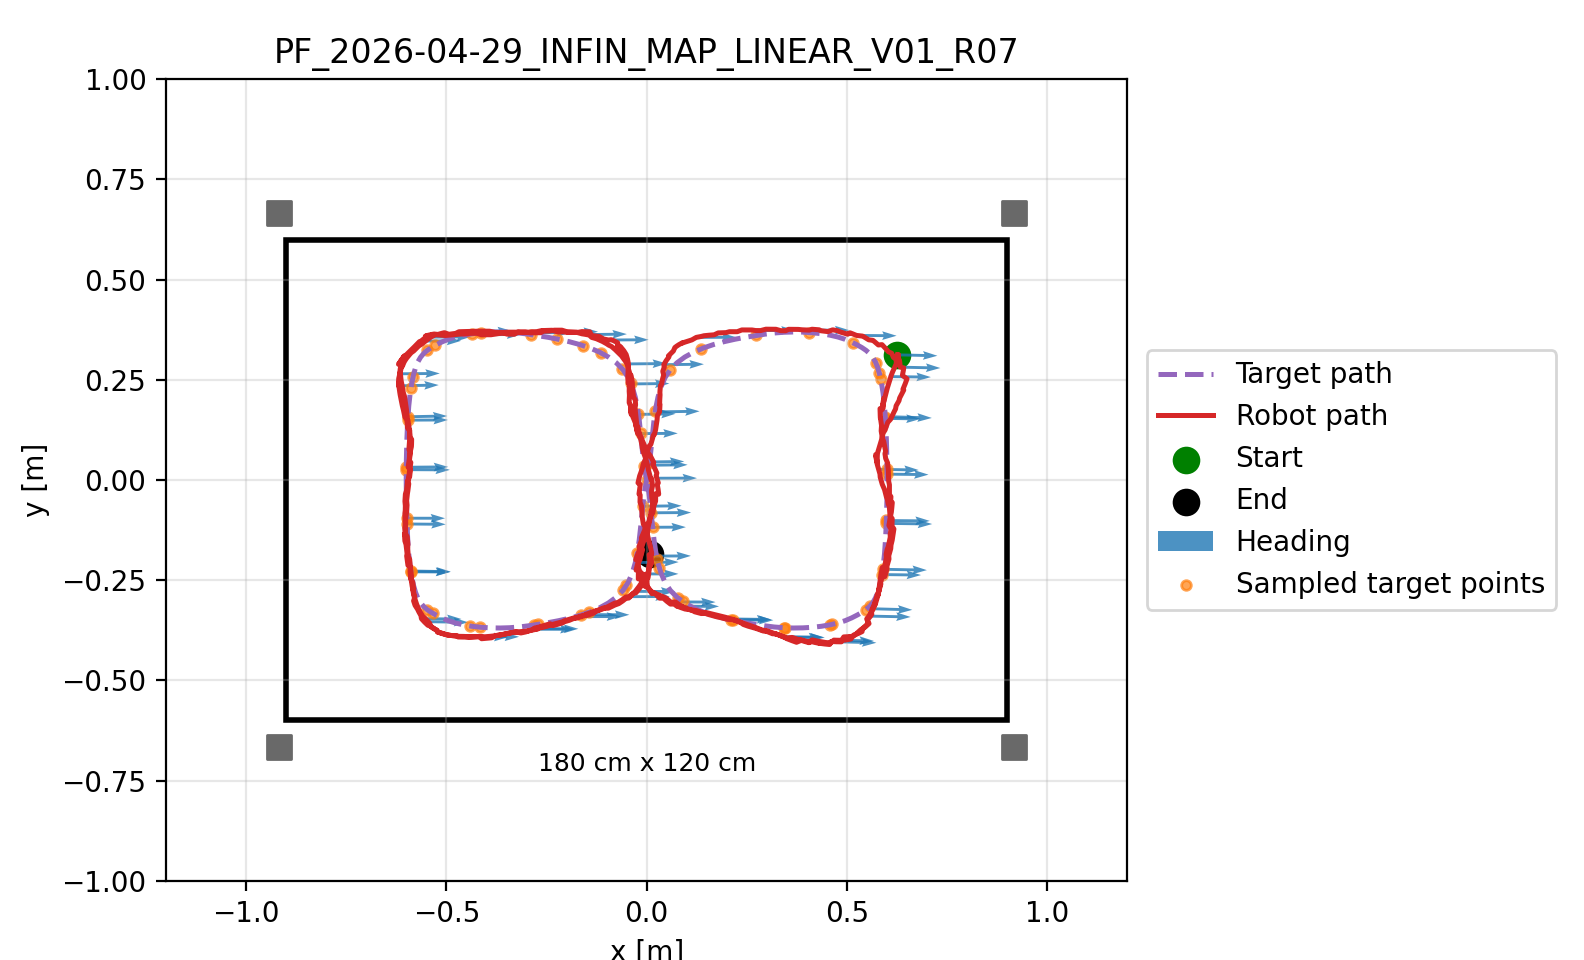
\includegraphics[width=0.7\linewidth]{IMG/controller/LIN/LIN_03_xy_map.png}
        \caption{LIN\_03 xy map}
        \label{fig:LIN_03_xy_map}
    \end{subfigure}

    \vspace{0.5em}

    \begin{subfigure}{\textwidth}
        \centering
        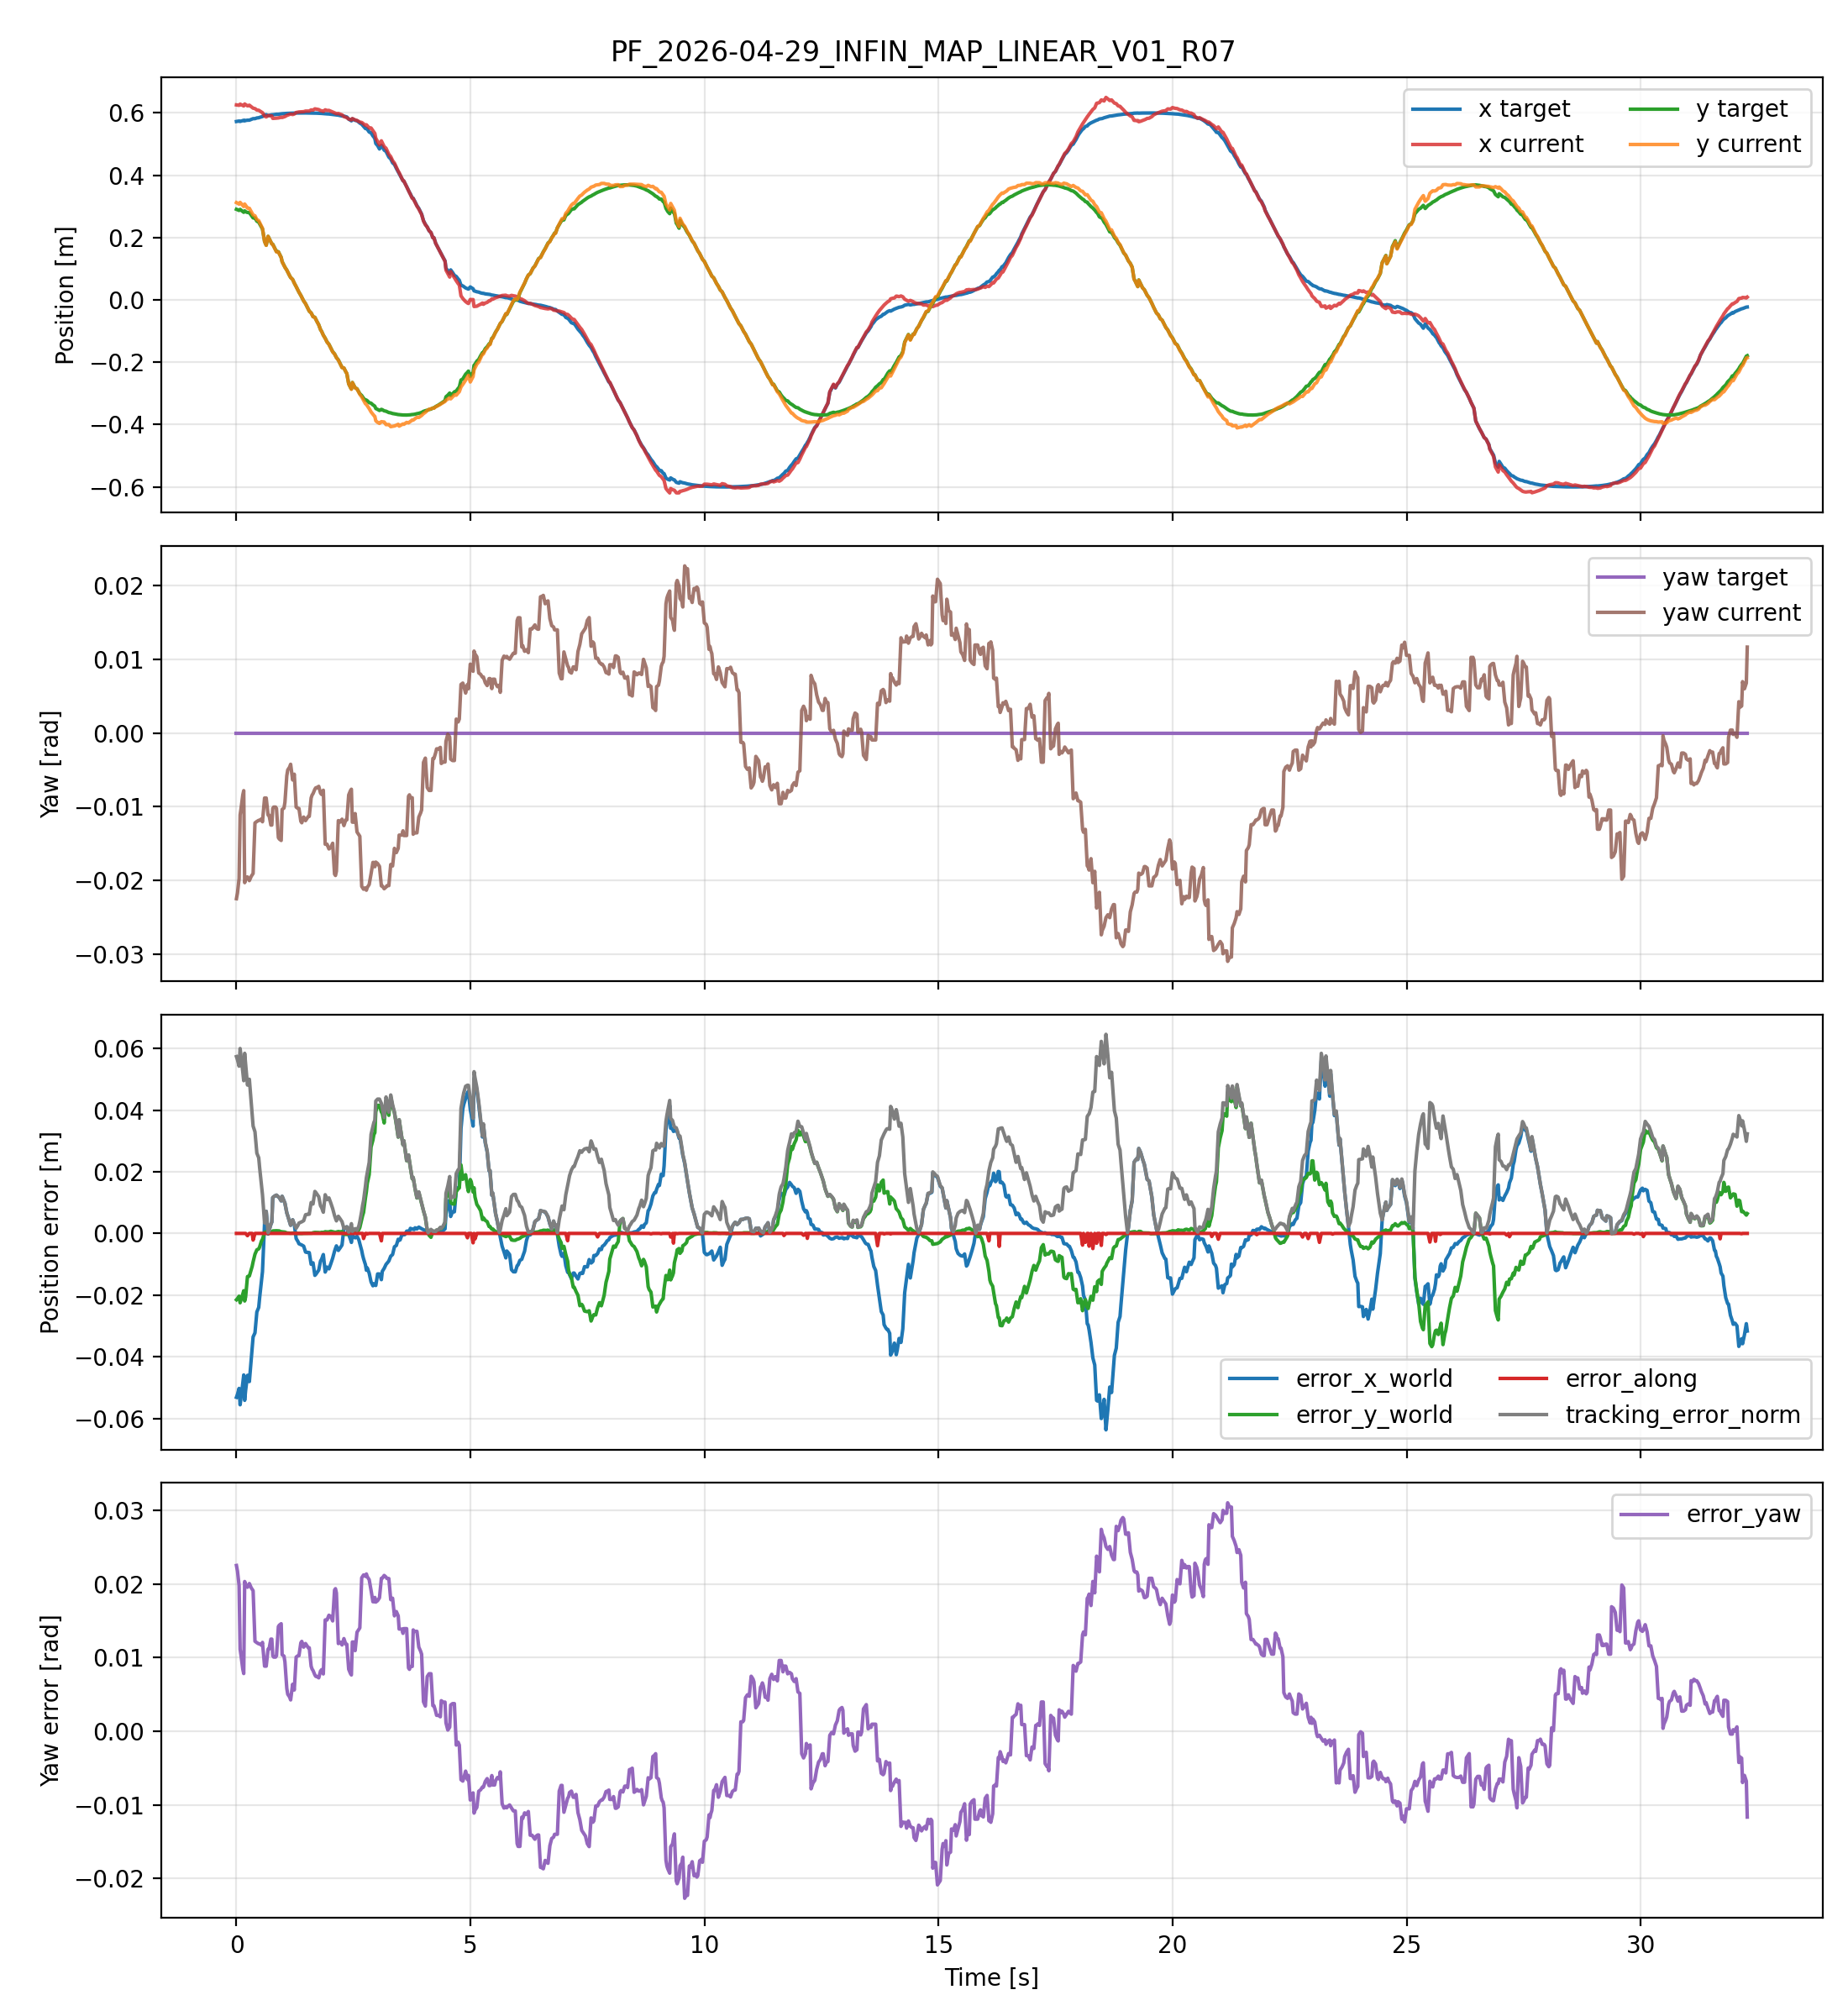
\includegraphics[width=0.7\linewidth]{IMG/controller/LIN/LIN_03_target_tracking_and_errors.png}
        \caption{LIN\_03 tracking and errors}
        \label{fig:LIN_03_tracking_and_errors}
    \end{subfigure}
    
    \vspace{0.5em}
    \caption{Experimental results for LIN\_03 scenario.} 
    \label{fig:LIN_03_general}
\end{figure}

\newpage
\begin{figure}[H]
    \centering
    \begin{subfigure}{\textwidth}
        \centering
        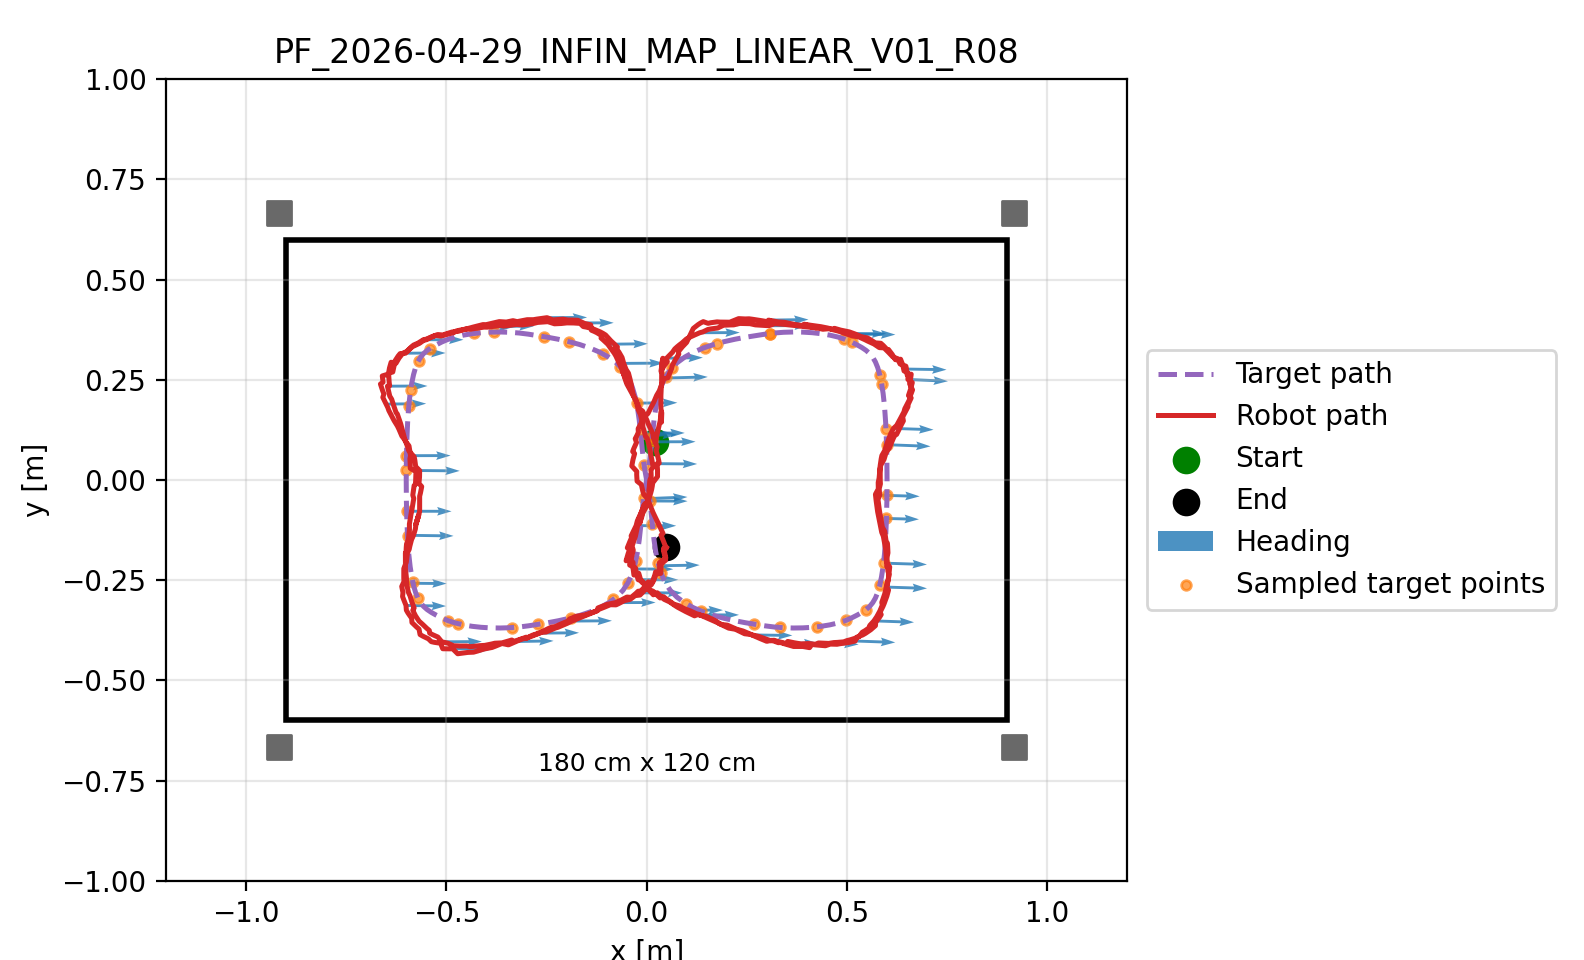
\includegraphics[width=0.7\linewidth]{IMG/controller/LIN/LIN_04_xy_map.png}
        \caption{LIN\_04 xy map}
        \label{fig:LIN_04_xy_map}
    \end{subfigure}

    \vspace{0.5em}

    \begin{subfigure}{\textwidth}
        \centering
        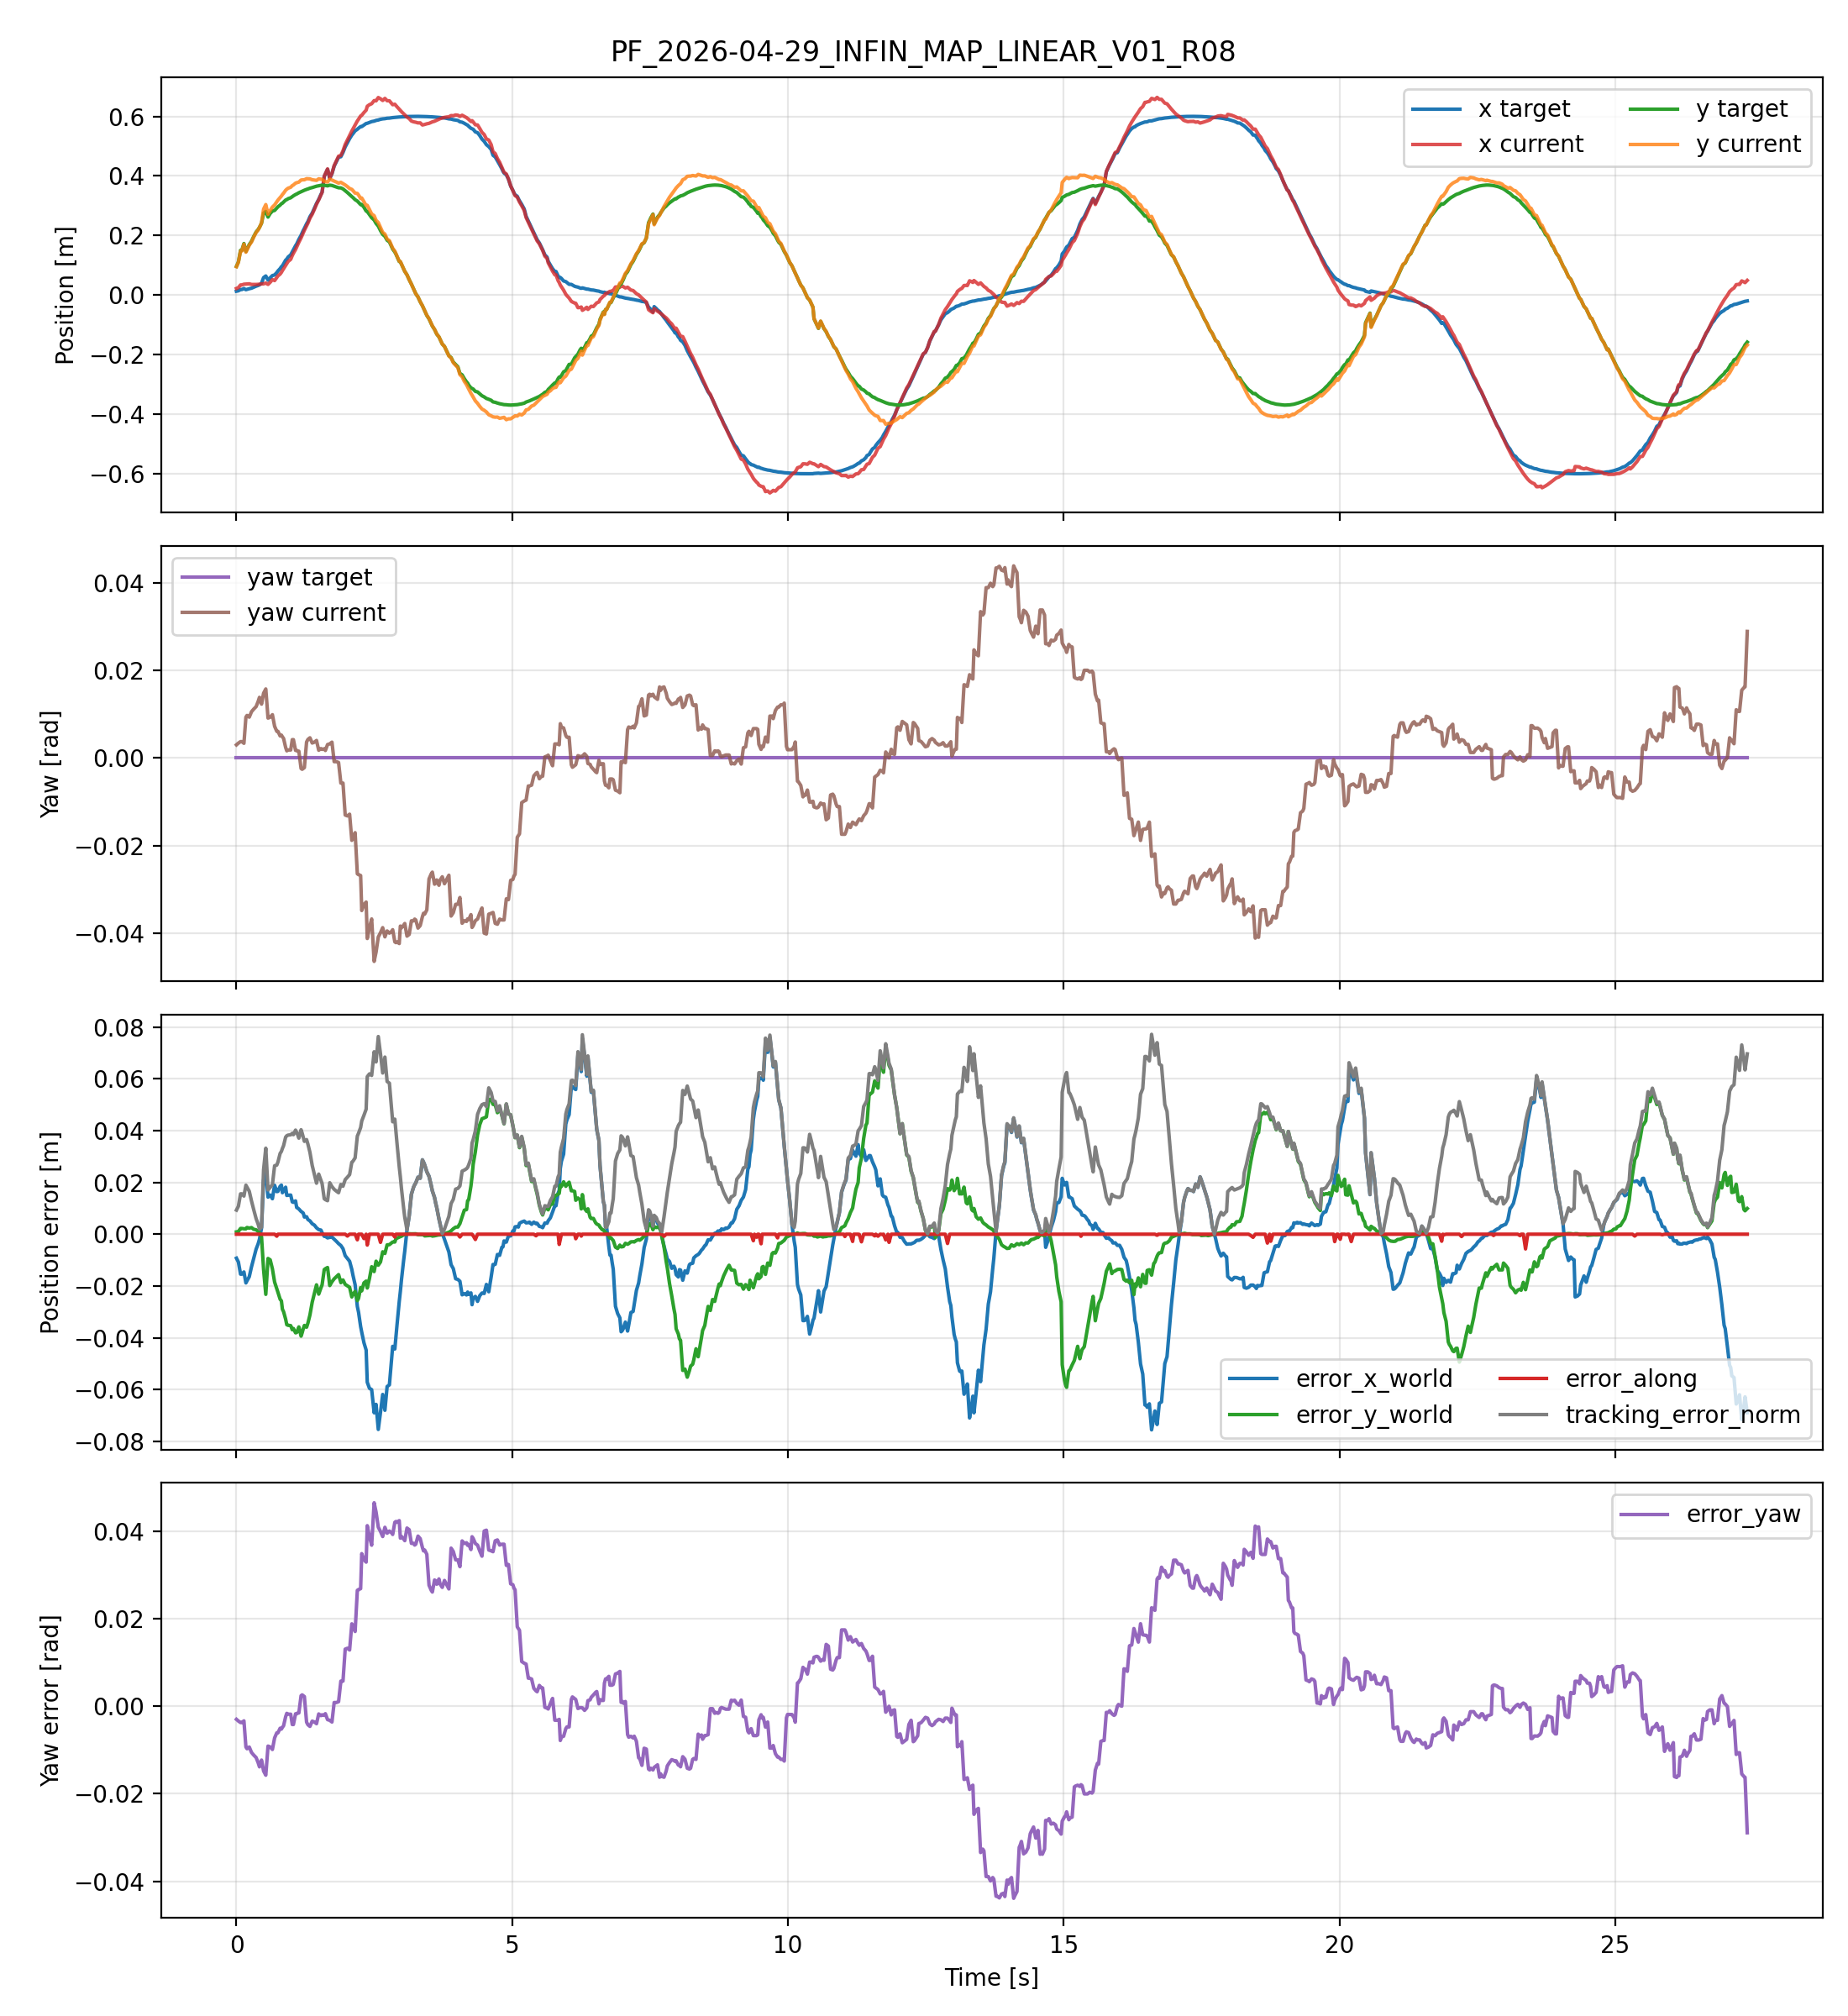
\includegraphics[width=0.7\linewidth]{IMG/controller/LIN/LIN_04_target_tracking_and_errors.png}
        \caption{LIN\_04 tracking and errors}
        \label{fig:LIN_04_tracking_and_errors}
    \end{subfigure}
    
    \vspace{0.5em}
    \caption{Experimental results for LIN\_04 scenario.} 
    \label{fig:LIN_04_general}
\end{figure}

\newpage
\begin{figure}[H]
    \centering
    \begin{subfigure}{\textwidth}
        \centering
        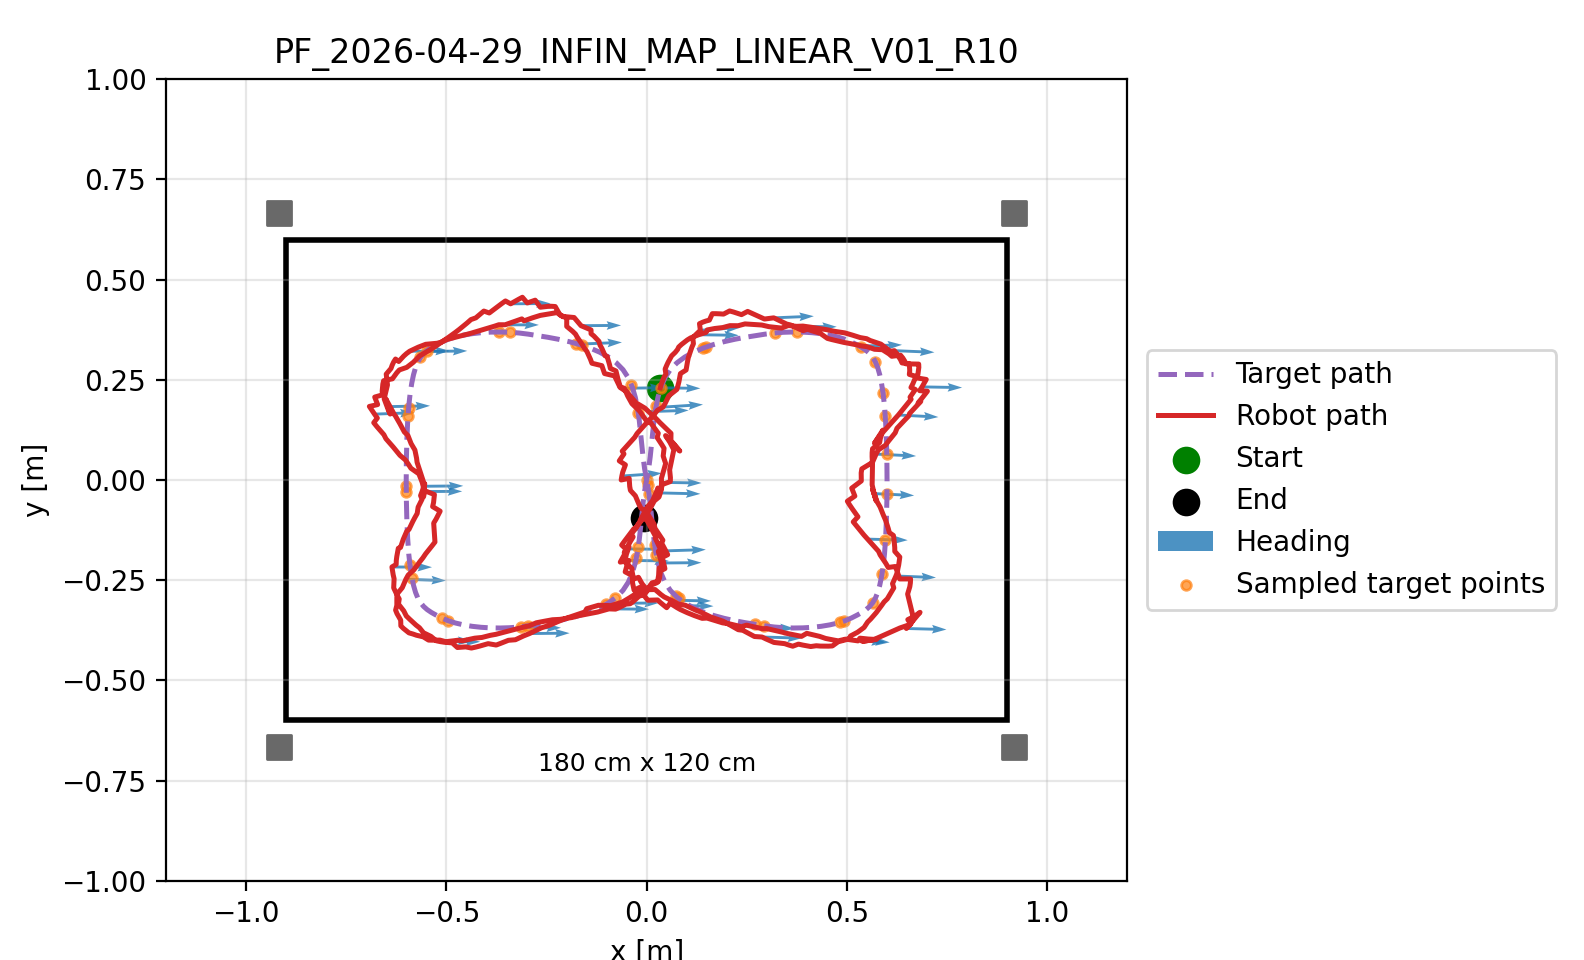
\includegraphics[width=0.7\linewidth]{IMG/controller/LIN/LIN_05_xy_map.png}
        \caption{LIN\_05 xy map}
        \label{fig:LIN_05_xy_map}
    \end{subfigure}

    \vspace{0.5em}

    \begin{subfigure}{\textwidth}
        \centering
        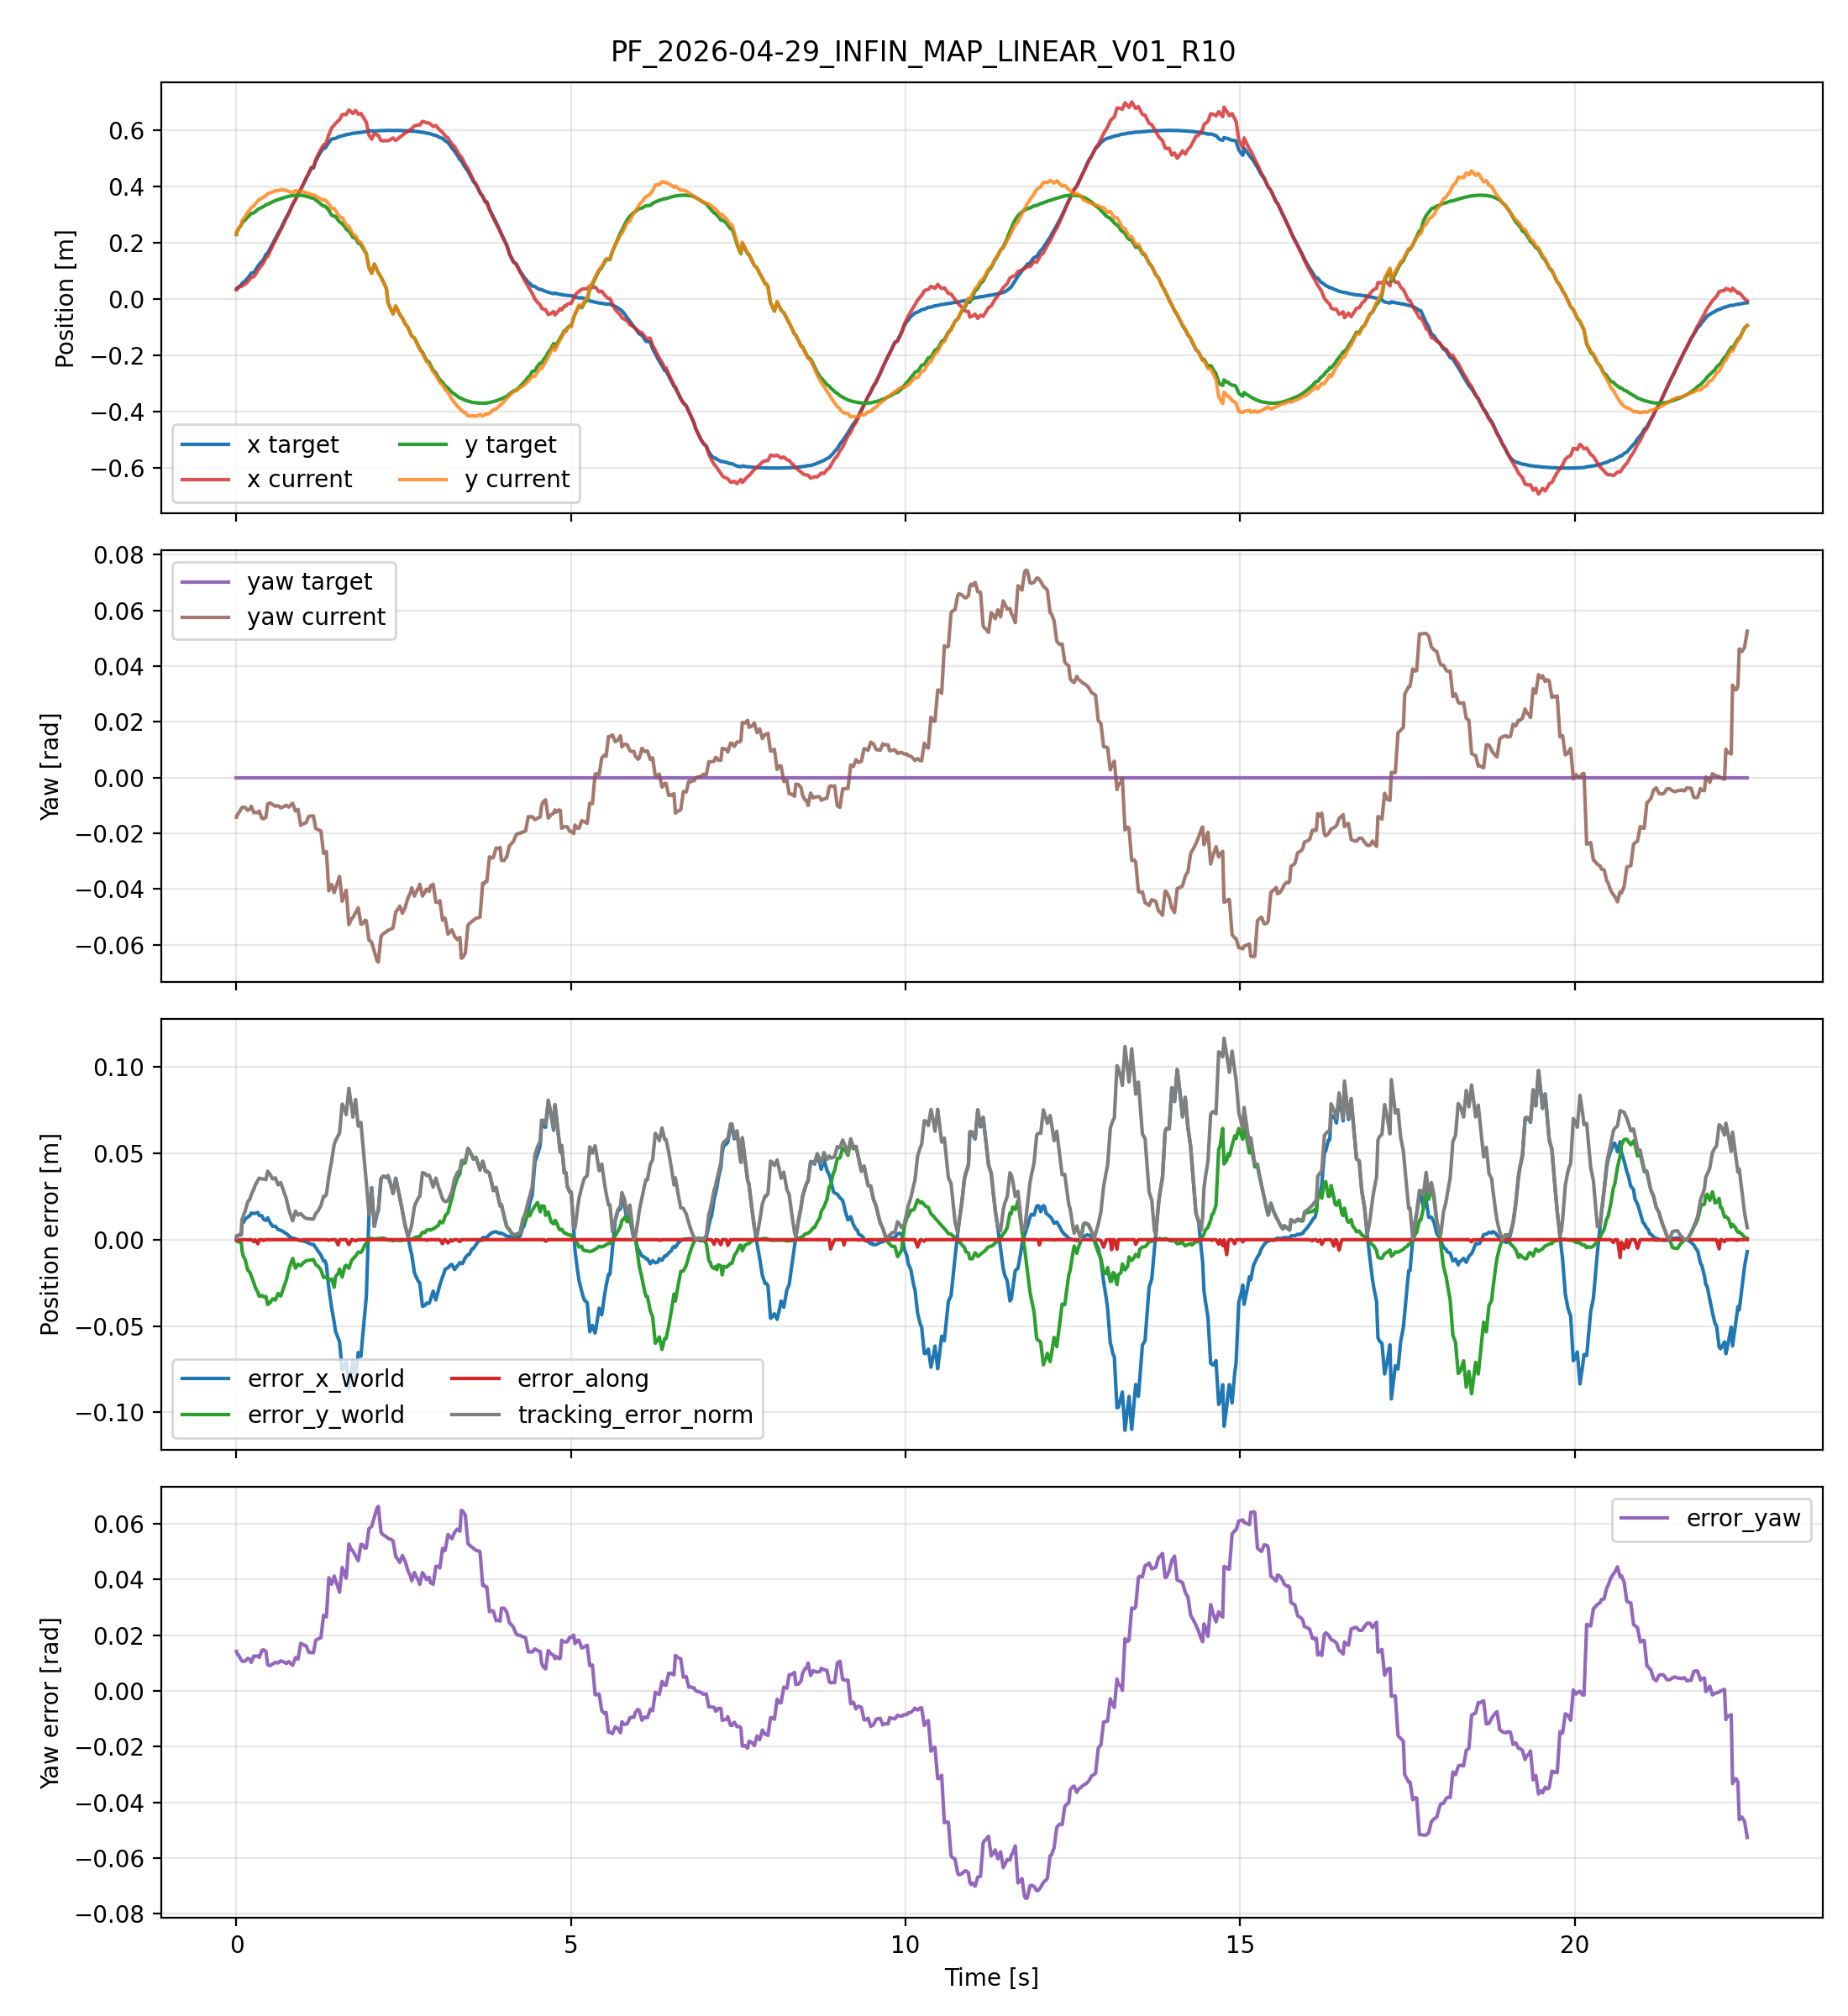
\includegraphics[width=0.7\linewidth]{IMG/controller/LIN/LIN_05_target_tracking_and_errors.png}
        \caption{LIN\_05 tracking and errors}
        \label{fig:LIN_05_tracking_and_errors}
    \end{subfigure}
    
    \vspace{0.5em}
    \caption{Experimental results for LIN\_05 scenario.} 
    \label{fig:LIN_05_general}
\end{figure}

% Section to append to Chapter 6 after the Linear Segment controller.
% Required packages: booktabs, float, subcaption.

% Section to append to Chapter 6 after the Linear Segment controller.
% Required packages: booktabs, float, subcaption.
% Code excerpts use the standard LaTeX verbatim environment.

\section{Nonlinear Model Predictive Contouring Controller}
\label{sec:nonlinear_mpcc_controller}

This section describes the predictive controller used in the experimental.  The objective of the controller is not only to
reduce the instantaneous Cartesian error with respect to a moving point, but to
choose a velocity command by considering the future evolution of the robot over a
short horizon.  This is the main difference with the previous geometric
controllers: the command is selected by balancing path accuracy, path
progression, command effort and command smoothness in the same optimization
problem.

The formulation is inspired by MPC trajectory-tracking approaches for
omnidirectional mobile robots.  In those approaches a model of the robot is used
to predict the future motion, and an optimal control problem is solved at each
control period.  Smooth parametric references, such as B-Spline trajectories, are
particularly suitable for MPC because the reference can be evaluated at any point
of the prediction horizon and the local path geometry can be used inside the
cost function.  In this work the reference is treated as a geometric path rather
than as a purely time-indexed trajectory.  The progression along the path is
represented by the curvilinear coordinate \(\gamma\), so the controller can
separate lateral path error from advancement along the curve.

The controller follows the same cascade architecture used in the rest of the
ROS2 stack.  The high-level node receives the estimated pose in the
\texttt{map} frame, evaluates the reference path, computes a planar velocity
command and publishes a \texttt{geometry\_msgs/Twist} message on
\texttt{cmd\_vel}.  The lower ROS2 driver and the ESP32 firmware then convert
this velocity reference into wheel commands and motor voltages.

\subsection{Geometric Path Representation}

The reference path is represented by a sequence of points loaded from a CSV file.
The implementation stores the cumulative distance along the polyline, which is
used as the path coordinate \(\gamma\).  Given \(\gamma\), the function
\texttt{sampleAt} finds the corresponding segment, interpolates the reference
position and computes the local tangent:

\begin{verbatim}
PathSample sampleAt(double gamma) const
{
  ...
  sample.x = a.x + ratio * (b.x - a.x);
  sample.y = a.y + ratio * (b.y - a.y);
  sample.tangent_x = (b.x - a.x) / segment_length;
  sample.tangent_y = (b.y - a.y) / segment_length;
  ...
}
\end{verbatim}

The tangent vector is therefore
\begin{equation}
    \mathbf{t}(\gamma)=
    \begin{bmatrix}
        t_x(\gamma) & t_y(\gamma)
    \end{bmatrix}^{T},
\end{equation}
while the normal vector is obtained as
\begin{equation}
    \mathbf{n}(\gamma)=
    \begin{bmatrix}
        -t_y(\gamma) & t_x(\gamma)
    \end{bmatrix}^{T}.
\end{equation}
This same geometric representation is used by the Linear Segment controller and
is the natural basis for the MPCC formulation, because contouring and lag errors
are defined with respect to the tangent and normal directions of the path.

\subsection{Predictive Model}

The predicted state is defined as
\begin{equation}
    \mathbf{x}_k =
    \begin{bmatrix}
        x_k & y_k & \psi_k & \gamma_k
    \end{bmatrix}^{T},
\end{equation}
where \((x_k,y_k,\psi_k)\) is the predicted robot pose and \(\gamma_k\) is the
predicted curvilinear coordinate along the path.  The control vector is
\begin{equation}
    \mathbf{u}_k =
    \begin{bmatrix}
        v_{x,k} & v_{y,k} & \omega_k & \dot{\gamma}_k
    \end{bmatrix}^{T}.
\end{equation}
The first three variables are the body-frame velocity command sent to the robot,
whereas \(\dot{\gamma}_k\) controls the virtual advancement of the reference
point along the path.

The prediction model is the discrete-time kinematic model of a holonomic mobile
robot:
\begin{equation}
\begin{aligned}
    x_{k+1} &= x_k + \Delta t
    \left(\cos\psi_k\,v_{x,k}-\sin\psi_k\,v_{y,k}\right), \\
    y_{k+1} &= y_k + \Delta t
    \left(\sin\psi_k\,v_{x,k}+\cos\psi_k\,v_{y,k}\right), \\
    \psi_{k+1} &= \mathrm{wrapToPi}(\psi_k + \Delta t\,\omega_k), \\
    \gamma_{k+1} &= \gamma_k + \Delta t\,\dot{\gamma}_k .
\end{aligned}
\end{equation}
This model is intentionally simple: it assumes that the omnidirectional platform
can track the commanded planar velocity directly.  Therefore, wheel dynamics,
slip, actuator dead zones and low-level loop delays are not part of the
prediction model.  In the experimental tests the prediction step is
\(\Delta t=0.08~\mathrm{s}\).  The horizon is usually \(N=12\), corresponding to
a prediction window of approximately \(0.96~\mathrm{s}\), while the final test
uses \(N=14\), corresponding to approximately \(1.12~\mathrm{s}\).

\subsection{Contouring and Lag Errors}

At each predicted step the path is sampled at \(\gamma_k\).  Let
\(\mathbf{p}_k=[x_k\;y_k]^T\) be the predicted robot position and
\(\mathbf{p}_r(\gamma_k)\) the sampled reference point.  The position error is
projected onto the tangent and normal directions:
\begin{equation}
    e_{l,k} =
    \left(\mathbf{p}_k-\mathbf{p}_r(\gamma_k)\right)^T
    \mathbf{t}(\gamma_k),
    \qquad
    e_{c,k} =
    \left(\mathbf{p}_k-\mathbf{p}_r(\gamma_k)\right)^T
    \mathbf{n}(\gamma_k).
\end{equation}
The lag error \(e_l\) measures whether the predicted robot position is ahead of
or behind the virtual reference point along the path.  The contouring error
\(e_c\) measures the lateral deviation from the path and is the most important
quantity for geometric path following.  The heading error is
\begin{equation}
    e_{\psi,k}=\mathrm{wrapToPi}(\psi_r(\gamma_k)-\psi_k).
\end{equation}

The same decomposition can be seen in the available path-following code used for
the Linear Segment controller.  The controller computes the tangent, builds the
normal vector, and projects the Cartesian error onto both directions:

\begin{verbatim}
const double normal_x = -command.target.tangent_y;
const double normal_y = command.target.tangent_x;
const double error_along =
  dx_world * command.target.tangent_x + dy_world * command.target.tangent_y;
const double error_lateral = dx_world * normal_x + dy_world * normal_y;
\end{verbatim}

For the MPCC, these same geometric quantities are evaluated not only at the
current pose, but at every predicted state along the horizon.

\subsection{Cost Function}

The stage cost minimized along the horizon is composed of tracking, progress,
effort and smoothness terms:
\begin{equation}
\begin{aligned}
    J_k =&
    q_c e_{c,k}^{2}
    + q_l e_{l,k}^{2}
    + q_{\psi} e_{\psi,k}^{2}
    - q_p \dot{\gamma}_k \\
    &+ r_{v_x} v_{x,k}^{2}
    + r_{v_y} v_{y,k}^{2}
    + r_{\omega} \omega_k^{2}
    + r_{\dot{\gamma}} \dot{\gamma}_k^{2} \\
    &+ r_{\Delta v_x}\Delta v_{x,k}^{2}
    + r_{\Delta v_y}\Delta v_{y,k}^{2}
    + r_{\Delta\omega}\Delta\omega_k^{2}
    + r_{\Delta\dot{\gamma}}\Delta\dot{\gamma}_k^{2}.
\end{aligned}
\end{equation}
The terms \(q_c\), \(q_l\) and \(q_{\psi}\) penalize geometric tracking errors.
The negative term \(-q_p\dot{\gamma}_k\) rewards advancement along the path.  The
\(r\) terms penalize large velocity commands, while the \(r_\Delta\) terms
penalize command increments.  Penalizing increments is important in practice
because it reduces abrupt changes in \texttt{cmd\_vel} without forcing the
absolute velocity to be unnecessarily small.  A terminal cost is also added to
the last predicted contouring and lag errors, so the final state of the rollout
is encouraged to remain close to the path.

\subsection{Implementation Structure}

The ROS2 path-following node is organized around a common control pipeline:
receive the pose, compute a \texttt{ControlCommand}, and publish the final
\texttt{Twist}.  In the public repository version, the dispatcher selects between
\texttt{linear\_segment} and \texttt{moving\_reference\_p}:

\begin{verbatim}
void runFollow(const rclcpp::Time & stamp, double dt)
{
  ControlCommand command = controller_mode_ == "linear_segment" ?
    computeLinearSegmentCommand() :
    computeMovingReferenceCommand(dt);
  publishCommand(stamp, dt, command);
}
\end{verbatim}

The MPCC controller follows the same interface: it must return a
\texttt{ControlCommand} containing the selected body-frame velocities and the
predicted path advancement.  Conceptually, the dispatcher becomes:

\begin{verbatim}
if (controller_mode_ == "linear_segment") {
  command = computeLinearSegmentCommand();
} else if (controller_mode_ == "moving_reference_p") {
  command = computeMovingReferenceCommand(dt);
} else if (controller_mode_ == "nonlinear_mpcc") {
  command = computeNonlinearMpccCommand(dt);
}
\end{verbatim}

The sampled MPCC implementation can be summarized by the following pseudo-code:

\begin{verbatim}
best_cost = +infinity
best_command = previous_command

for vx in sampled_vx:
  for vy in sampled_vy:
    for omega in sampled_omega:
      for gamma_dot in sampled_gamma_dot:
        x_pred = current_x
        y_pred = current_y
        psi_pred = current_yaw
        gamma_pred = current_gamma
        cost = 0

        for k = 0 ... N-1:
          sample = sampleAt(gamma_pred)
          t = sample.tangent
          n = [-t.y, t.x]

          e_l = dot([x_pred,y_pred] - sample.position, t)
          e_c = dot([x_pred,y_pred] - sample.position, n)
          e_psi = wrapToPi(sample.yaw - psi_pred)

          cost += stageCost(e_c, e_l, e_psi,
                            vx, vy, omega, gamma_dot,
                            previous_command)

          x_pred += dt * (cos(psi_pred)*vx - sin(psi_pred)*vy)
          y_pred += dt * (sin(psi_pred)*vx + cos(psi_pred)*vy)
          psi_pred = wrapToPi(psi_pred + dt * omega)
          gamma_pred += dt * gamma_dot

        cost += terminalCost(e_c, e_l)

        if cost < best_cost:
          best_cost = cost
          best_command = [vx, vy, omega, gamma_dot]
\end{verbatim}

After the best candidate is selected, it is published through the same output
stage used by the other controllers.  The current node adds feedforward and
feedback terms, saturates the velocities and publishes \texttt{cmd\_vel}:

\begin{verbatim}
cmd.linear.x = clamp(cmd_vx_raw, -max_linear_x_, max_linear_x_);
cmd.linear.y = clamp(cmd_vy_raw, -max_linear_y_, max_linear_y_);
cmd.angular.z = clamp(cmd_w_raw, -max_angular_z_, max_angular_z_);
pub_cmd_vel_->publish(cmd);
\end{verbatim}

This implementation choice avoids the need for an external nonlinear optimizer
and is deterministic, but the result depends on the sampling resolution.  A
coarse grid is computationally cheap but may produce quantized commands, whereas
a dense grid improves the approximation at the cost of a higher computation
time.

\subsection{Limitations and Possible Improvements}

The main limitations of this first predictive formulation are:
\begin{itemize}
    \item the prediction model neglects wheel dynamics, actuator delay, wheel
    slip, friction and the transient response of the low-level velocity loop;
    \item the command is selected on a finite grid, so the solution is only an
    approximation of the continuous optimum;
    \item the same candidate command is kept constant during the whole rollout,
    which reduces computation time but limits the richness of the predicted
    control sequence;
    \item the controller depends directly on the pose estimate, so localization
    drift appears as contouring and lag error;
    \item obstacle constraints are not included, therefore the controller is a
    path-following controller and not a complete local planner.
\end{itemize}

Future work should focus on a continuous nonlinear solver, optimization of a full
command sequence instead of a constant command, curvature-dependent velocity
limits, adaptive progress weights, explicit actuator-delay compensation and
uncertainty-aware localization handling.  The current implementation is
therefore best interpreted as an experimental predictive baseline: it shows how
tracking, progress and smoothness can be traded off explicitly, but it still
requires further tuning before it can be considered superior to a simpler and
well-tuned geometric controller in all metrics.

\subsection{Test Parameters and Results}

\noindent
\textbf{Test legend:}
\begin{itemize}
    \item \textbf{MPC-01}: \texttt{PF\_2026-05-11\_INFIN\_MAP\_MPCC\_V01\_R01};
    \item \textbf{MPC-02}: \texttt{PF\_2026-05-11\_INFIN\_MAP\_MPCC\_V01\_R02};
    \item \textbf{MPC-03}: \texttt{PF\_2026-05-11\_INFIN\_MAP\_MPCC\_V01\_R03};
    \item \textbf{MPC-04}: \texttt{PF\_2026-05-11\_INFIN\_MAP\_MPCC\_V01\_R04};
    \item \textbf{MPC-05}: \texttt{PF\_2026-05-11\_INFIN\_MAP\_MPCC\_V01\_R05};
    \item \textbf{MPC-06}: \texttt{PF\_2026-05-11\_INFIN\_MAP\_MPCC\_V01\_R06}.
\end{itemize}

The following parameters are common to all tests: path \texttt{INFIN}, reference frame
\texttt{MAP}, controller mode \texttt{nonlinear\_mpcc}, fixed heading mode.

\begin{table}[H]
\centering
\caption{Main characteristic parameters of the selected MPCC tests.}
\label{tab:mpcc_characteristic_parameters}
\scriptsize
\setlength{\tabcolsep}{3pt}
\renewcommand{\arraystretch}{1.05}
\begin{tabular}{lcccccc}
\toprule
\textbf{Parameter} &
\textbf{MPC-01} &
\textbf{MPC-02} &
\textbf{MPC-03} &
\textbf{MPC-04} &
\textbf{MPC-05} &
\textbf{MPC-06} \\
\midrule
Main configuration 
& Baseline 
& Slow/stable 
& Aggressive 
& Very aggressive 
& Aggressive curves 
& Extreme \\
\midrule
\(v_{x,\max}\) [m/s]          
& 0.25 & 0.18 & 0.35 & 0.50 & 0.60 & 0.70 \\
\(v_{y,\max}\) [m/s]          
& 0.25 & 0.18 & 0.35 & 0.50 & 0.60 & 0.70 \\
\(\omega_{\max}\) [rad/s]     
& 0.45 & 0.35 & 0.60 & 0.60 & 0.60 & 0.80 \\
\(\dot{\gamma}_{\max}\) [m/s] 
& 0.30 & 0.20 & 0.40 & 0.40 & 0.40 & 0.70 \\
\midrule
\(a_{x,\max}\) [m/s\(^2\)]    
& 0.60 & 0.40 & 0.90 & 0.90 & 0.90 & 1.80 \\
\(a_{y,\max}\) [m/s\(^2\)]    
& 0.60 & 0.40 & 0.90 & 0.90 & 0.90 & 1.80 \\
\(\dot{\omega}_{\max}\) [rad/s\(^2\)] 
& 1.20 & 0.80 & 1.60 & 1.60 & 1.60 & 2.50 \\
\(\ddot{\gamma}_{\max}\) [m/s\(^2\)] 
& 0.80 & 0.50 & 1.20 & 1.20 & 1.20 & 2.50 \\
\midrule
\(q_p\)                       
& 0.40 & 0.25 & 0.60 & 0.60 & 0.90 & 1.60 \\
\(q_c\)                       
& 20 & 20 & 20 & 20 & 20 & 18 \\
\(q_l\)                       
& 2 & 2 & 2 & 2 & 2 & 1 \\
\(q_{\psi}\)                  
& 1.0 & 1.0 & 1.0 & 1.0 & 1.0 & 0.6 \\
\midrule
\(r_{v_x}, r_{v_y}\)          
& 0.15 & 0.15 & 0.15 & 0.15 & 0.15 & 0.07 \\
\(r_{\omega}\)                
& 0.10 & 0.10 & 0.10 & 0.10 & 0.10 & 0.05 \\
\(r_{\dot{\gamma}}\)          
& 0.05 & 0.05 & 0.05 & 0.05 & 0.05 & 0.02 \\
\(r_{\Delta v_x}, r_{\Delta v_y}\) 
& 0.50 & 0.50 & 0.50 & 0.50 & 0.70 & 0.25 \\
\(r_{\Delta \omega}\)         
& 0.20 & 0.20 & 0.20 & 0.20 & 0.20 & 0.10 \\
\(r_{\Delta \dot{\gamma}}\)   
& 0.10 & 0.10 & 0.10 & 0.10 & 0.10 & 0.30 \\
\midrule
\(N\)                         
& 12 & 12 & 12 & 12 & 12 & 14 \\
\(\dot{\gamma}\) samples      
& 5 & 5 & 5 & 5 & 5 & 7 \\
\bottomrule
\end{tabular}
\end{table}

\begin{table}[H]
\centering
\caption{Compact notation used for vector parameters.}
\label{tab:mpcc_vector_parameters}
\scriptsize
\setlength{\tabcolsep}{4pt}
\renewcommand{\arraystretch}{1.05}
\begin{tabular}{ll}
\toprule
\textbf{Code} & \textbf{Values} \\
\midrule
A & \((r_{v_x}, r_{v_y}, r_{\omega}, r_{\dot{\gamma}})=(0.15,0.15,0.10,0.05)\) \\
B & \((r_{v_x}, r_{v_y}, r_{\omega}, r_{\dot{\gamma}})=(0.07,0.07,0.05,0.02)\) \\
C & \((r_{\Delta v_x}, r_{\Delta v_y}, r_{\Delta \omega}, r_{\Delta\dot{\gamma}})=(0.50,0.50,0.20,0.10)\) \\
D & \((r_{\Delta v_x}, r_{\Delta v_y}, r_{\Delta \omega}, r_{\Delta\dot{\gamma}})=(0.25,0.25,0.10,0.30)\) \\
S1 & \((v_x,v_y,\omega,\dot{\gamma})_{\mathrm{samples}}=(5,5,5,5)\) \\
S2 & \((v_x,v_y,\omega,\dot{\gamma})_{\mathrm{samples}}=(5,5,5,7)\) \\
\bottomrule
\end{tabular}
\end{table}

\begin{table}[H]
\centering
\caption{Nonlinear MPCC controller: experimental results of the selected tests.}
\label{tab:mpcc_experimental_results}
\scriptsize
\begin{tabular}{lcccccc}
\toprule
\textbf{Metric} &
\textbf{MPC-01} &
\textbf{MPC-02} &
\textbf{MPC-03} &
\textbf{MPC-04} &
\textbf{MPC-05} &
\textbf{MPC-06} \\
\midrule
Duration [s] & 54.46 & 32.39 & 50.40 & 29.53 & 35.39 & 21.53 \\
Samples & 818 & 487 & 757 & 444 & 532 & 324 \\
Mean sample time [s] & 0.0667 & 0.0667 & 0.0667 & 0.0667 & 0.0667 & 0.0667 \\
Real path length [m] & 9.5826 & 7.1290 & 7.0083 & 6.8210 & 9.4391 & 6.2836 \\
Final \(\gamma\) [m] & 2.1353 & 4.5252 & 4.5341 & 2.2472 & 2.2663 & 4.4428 \\
Path progress ratio \(r_{\gamma}\) & 0.4688 & 0.9935 & 0.9955 & 0.4934 & 0.4976 & 0.9754 \\
\(\mathrm{RMSE}_x\) [m] & 0.0202 & 0.0272 & 0.0153 & 0.0291 & 0.0368 & 0.0677 \\
\(\mathrm{RMSE}_y\) [m] & 0.0317 & 0.0440 & 0.0228 & 0.0487 & 0.0583 & 0.0934 \\
\(\mathrm{RMSE}_{\|e\|}\) [m] & 0.0376 & 0.0517 & 0.0274 & 0.0568 & 0.0689 & 0.1154 \\
Mean \(\|e\|\) [m] & 0.0333 & 0.0463 & 0.0253 & 0.0479 & 0.0614 & 0.1085 \\
Max \(\|e\|\) [m] & 0.0851 & 0.0970 & 0.0693 & 0.1323 & 0.1467 & 0.2102 \\
\(\mathrm{RMSE}_{\psi}\) [rad] & 0.0067 & 0.0092 & 0.0046 & 0.0108 & 0.0139 & 0.0294 \\
\(\mathrm{RMSE}_{e_{\parallel}}\) [m] & 0.0366 & 0.0503 & 0.0268 & 0.0552 & 0.0668 & 0.1104 \\
\(\mathrm{MAE}_{e_{\parallel}}\) [m] & 0.0321 & 0.0445 & 0.0244 & 0.0458 & 0.0589 & 0.1038 \\
\(\max |e_{\parallel}|\) [m] & 0.0851 & 0.0964 & 0.0693 & 0.1318 & 0.1455 & 0.2032 \\
\(\mathrm{IAE}_{e_{\parallel}}\) & 1.7487 & 1.4376 & 1.2276 & 1.3506 & 2.0827 & 2.2351 \\
\(\max |e_{\psi}|\) [rad] & 0.0413 & 0.0538 & 0.0151 & 0.0376 & 0.0473 & 0.0710 \\
Saturation ratio \(v_x\) & 0.0000 & 0.0000 & 0.0000 & 0.0000 & 0.0000 & 0.0000 \\
Saturation ratio \(v_y\) & 0.0000 & 0.0000 & 0.0000 & 0.0000 & 0.0000 & 0.0000 \\
Saturation ratio \(\omega\) & 0.0000 & 0.0000 & 0.0000 & 0.0000 & 0.0000 & 0.0000 \\
\bottomrule
\end{tabular}
\end{table}

The six MPCC tests show a clear progression in tuning.  \textbf{MPC-01} uses the
most conservative velocity limits and progress weight.  It remains stable and
has no command saturation, but it covers less than half of the path
\((r_{\gamma}=0.4688)\).  \textbf{MPC-02} and \textbf{MPC-03} increase the path
progression weight and the allowed velocity limits.  Both runs almost complete
the path, with \(r_{\gamma}=0.9935\) and \(r_{\gamma}=0.9955\), respectively.
Among all MPCC tests, \textbf{MPC-03} provides the best compromise in terms of
tracking accuracy, with \(\mathrm{RMSE}_x=0.0153~\mathrm{m}\),
\(\mathrm{RMSE}_y=0.0228~\mathrm{m}\), and the lowest yaw error
\(\mathrm{RMSE}_{\psi}=0.0046~\mathrm{rad}\).

\textbf{MPC-04} and \textbf{MPC-05} do not improve the tracking behaviour.  Even
though the actuator limits are increased, the path progression remains close to
half of the path and the position errors increase.  This suggests that simply
raising the available command range is not sufficient: the cost weights and the
prediction behaviour must remain balanced.  \textbf{MPC-06} is the most
aggressive configuration.  It uses a longer horizon, larger velocity limits,
lower effort penalties, and a much higher progress reward.  The robot again
covers almost the entire path \((r_{\gamma}=0.9754)\), but the tracking error
increases substantially, reaching \(\mathrm{RMSE}_{\|e\|}=0.1154~\mathrm{m}\).
This run is useful because it identifies the practical limit of this first MPCC
tuning: encouraging too much progression produces faster motion but degrades the
geometric quality of the trajectory.

\subsection{Experimental Figures}

\newpage
\begin{figure}[H]
    \centering
    \begin{subfigure}{\textwidth}
        \centering
        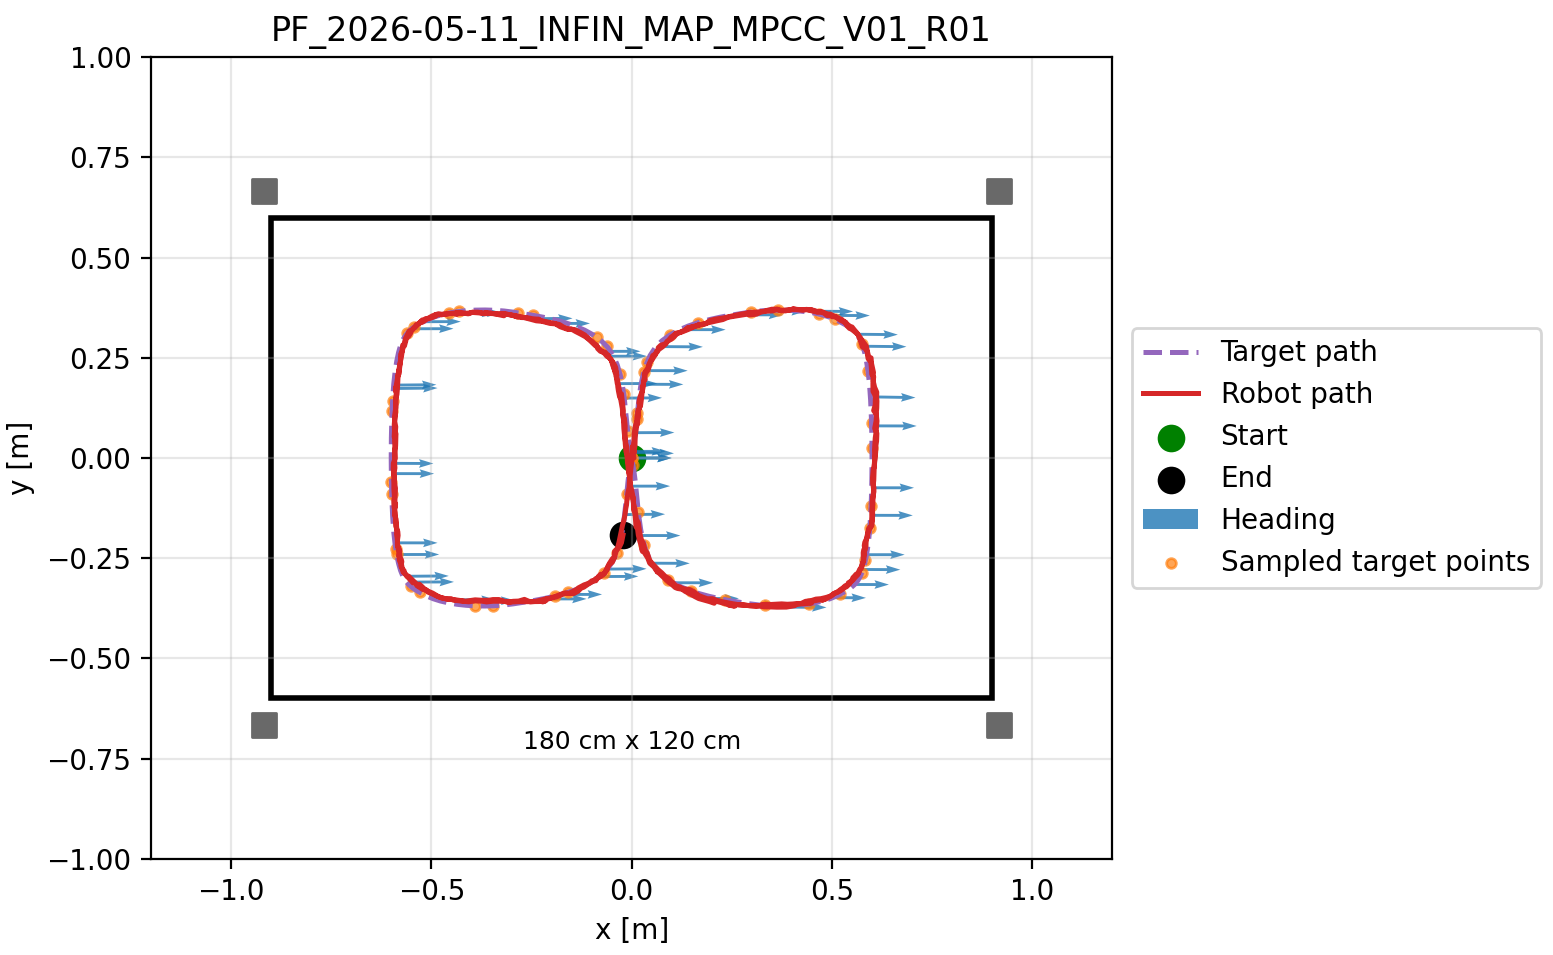
\includegraphics[width=0.7\linewidth]{IMG/controller/MPC/MPC_01_xy_map.png}
        \caption{MPC\_01 xy map}
        \label{fig:MPC_01_xy_map}
    \end{subfigure}

    \vspace{0.5em}

    \begin{subfigure}{\textwidth}
        \centering
        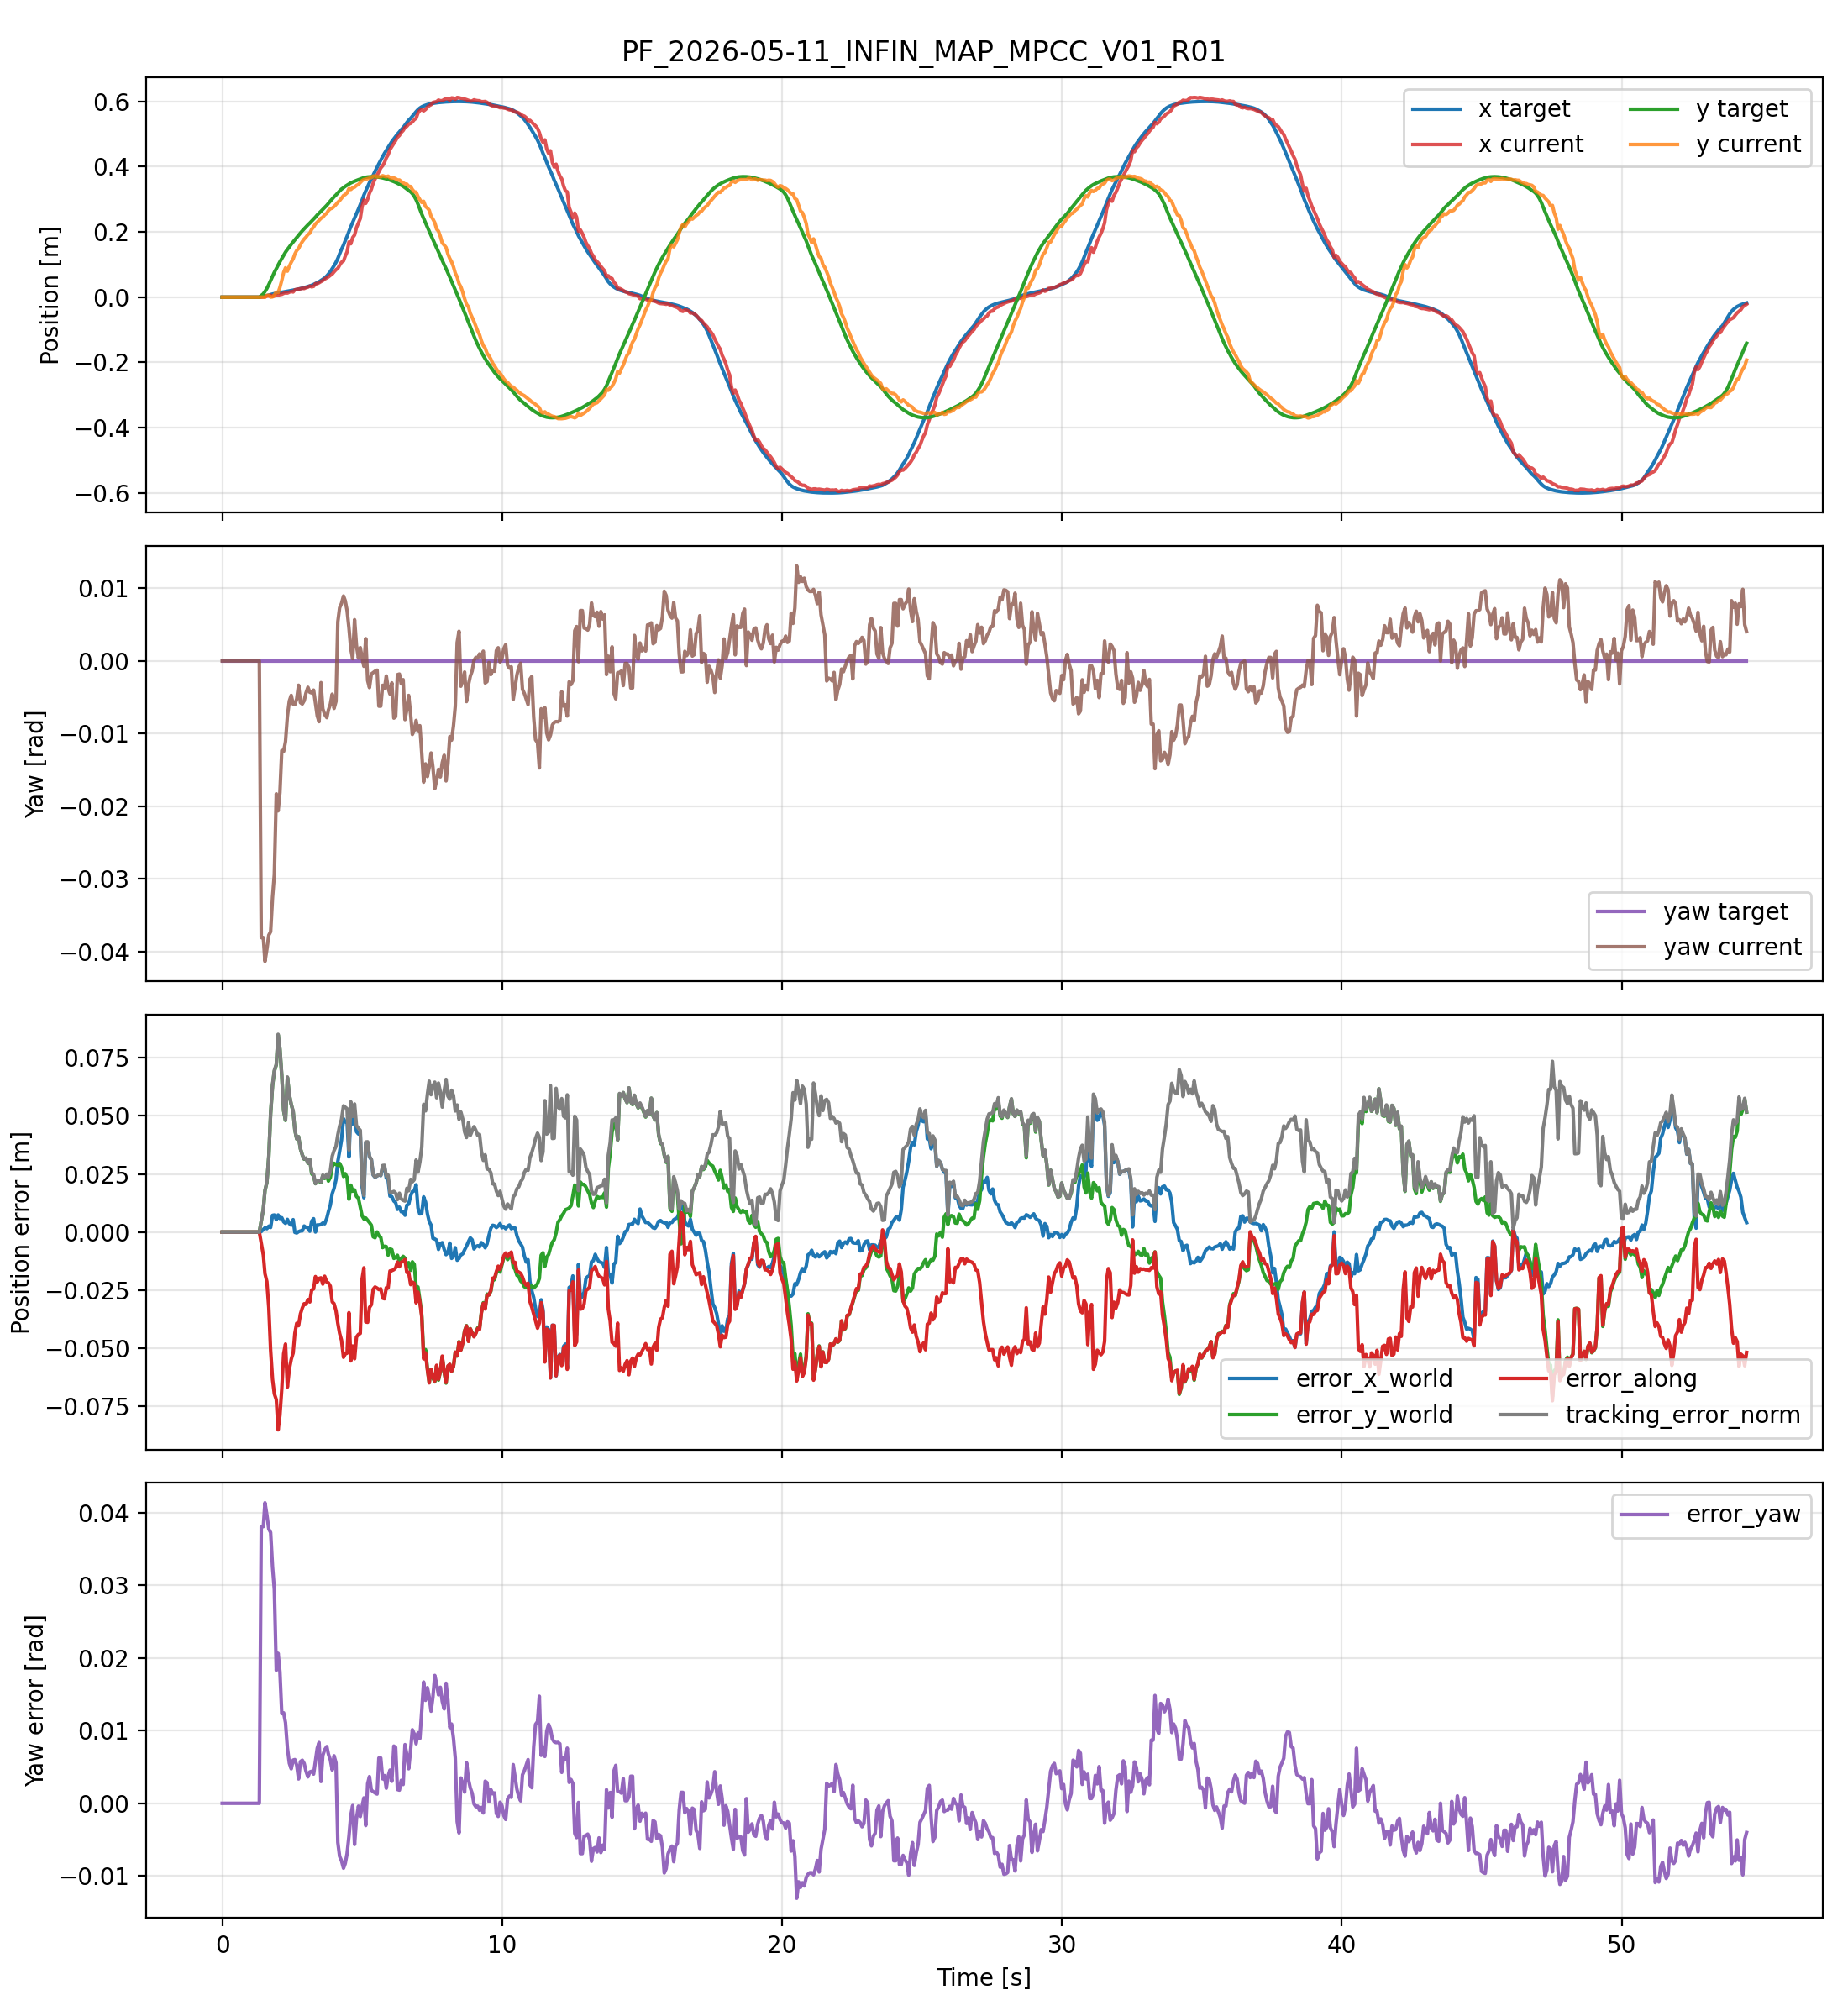
\includegraphics[width=0.7\linewidth]{IMG/controller/MPC/MPC_01_track_error.png}
        \caption{MPC\_01 tracking and errors}
        \label{fig:MPC_01_tracking_and_errors}
    \end{subfigure}
    \caption{Experimental results for MPC\_01 scenario.}
    \label{fig:MPC_01_general}
\end{figure}

\newpage
\begin{figure}[H]
    \centering
    \begin{subfigure}{\textwidth}
        \centering
        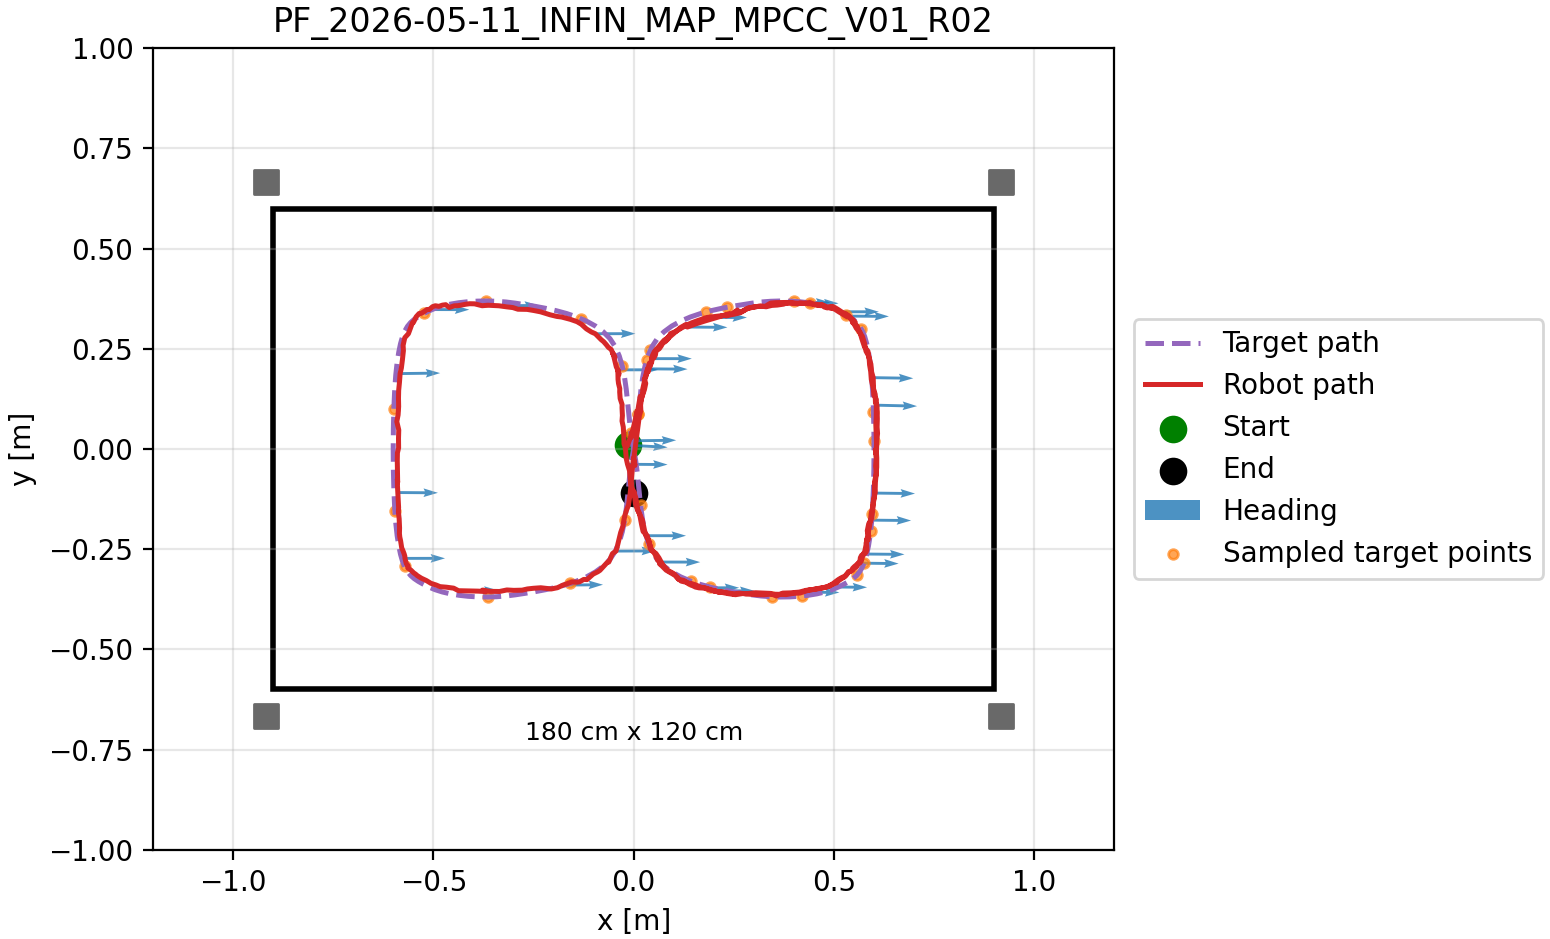
\includegraphics[width=0.7\linewidth]{IMG/controller/MPC/MPC_02_xy_map.png}
        \caption{MPC\_02 xy map}
        \label{fig:MPC_02_xy_map}
    \end{subfigure}

    \vspace{0.5em}

    \begin{subfigure}{\textwidth}
        \centering
        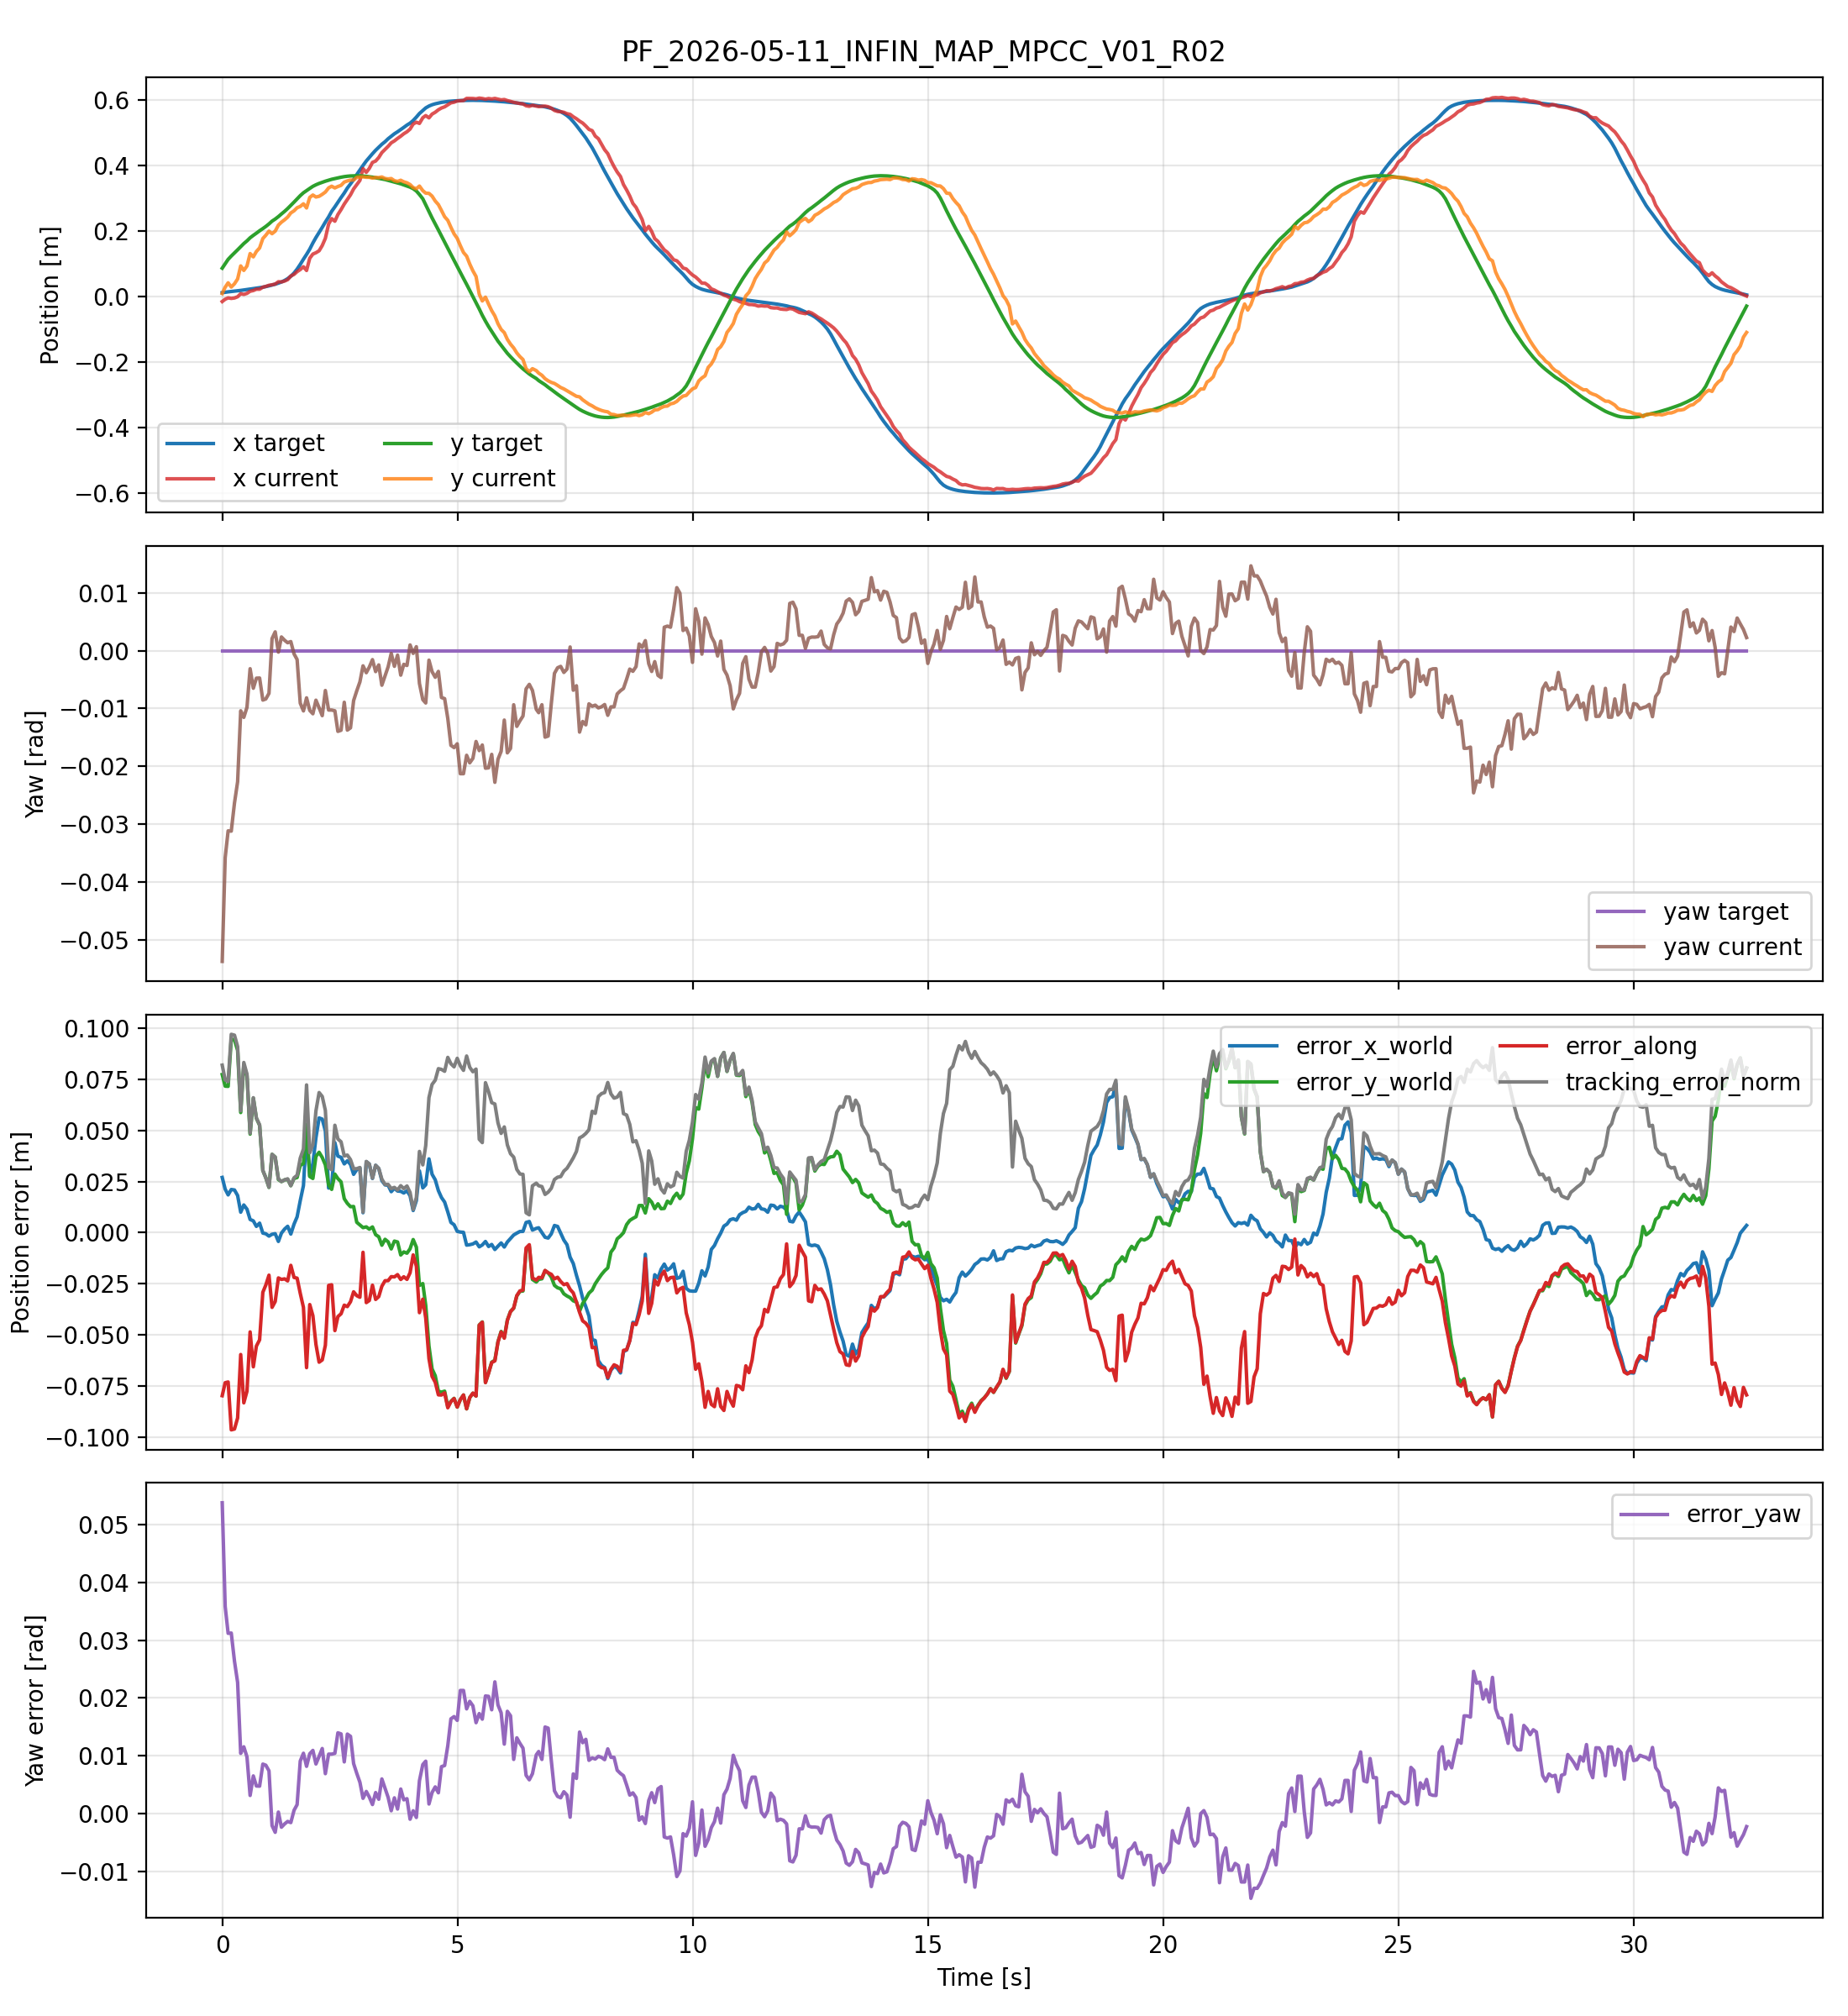
\includegraphics[width=0.7\linewidth]{IMG/controller/MPC/MPC_02_track_error.png}
        \caption{MPC\_02 tracking and errors}
        \label{fig:MPC_02_tracking_and_errors}
    \end{subfigure}
    \caption{Experimental results for MPC\_02 scenario.}
    \label{fig:MPC_02_general}
\end{figure}

\newpage
\begin{figure}[H]
    \centering
    \begin{subfigure}{\textwidth}
        \centering
        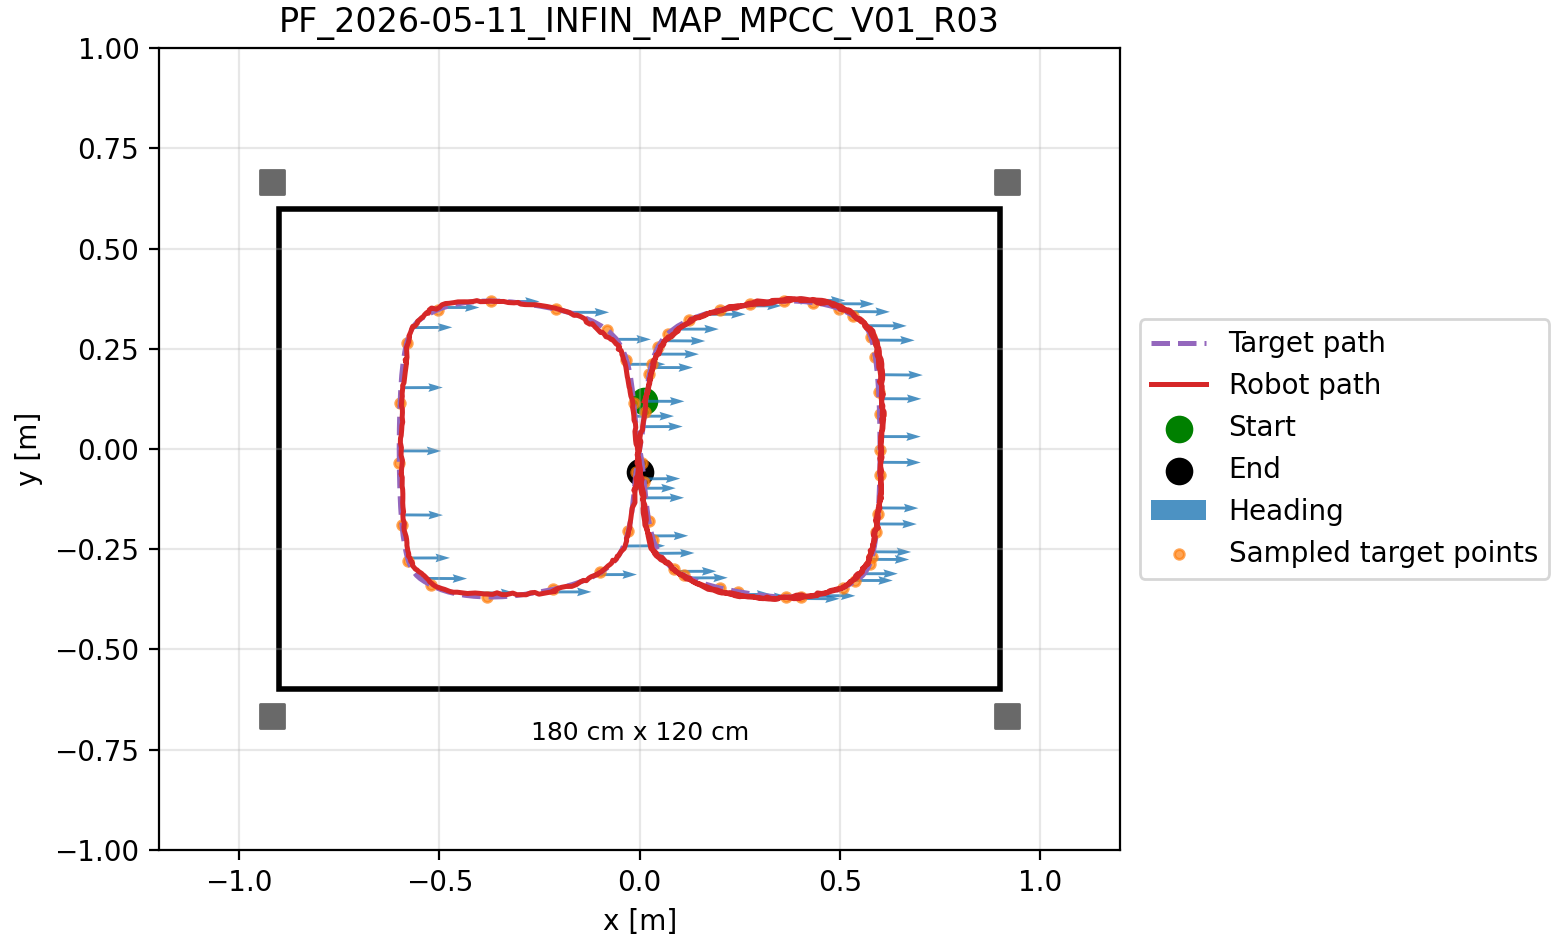
\includegraphics[width=0.7\linewidth]{IMG/controller/MPC/MPC_03_xy_map.png}
        \caption{MPC\_03 xy map}
        \label{fig:MPC_03_xy_map}
    \end{subfigure}

    \vspace{0.5em}

    \begin{subfigure}{\textwidth}
        \centering
        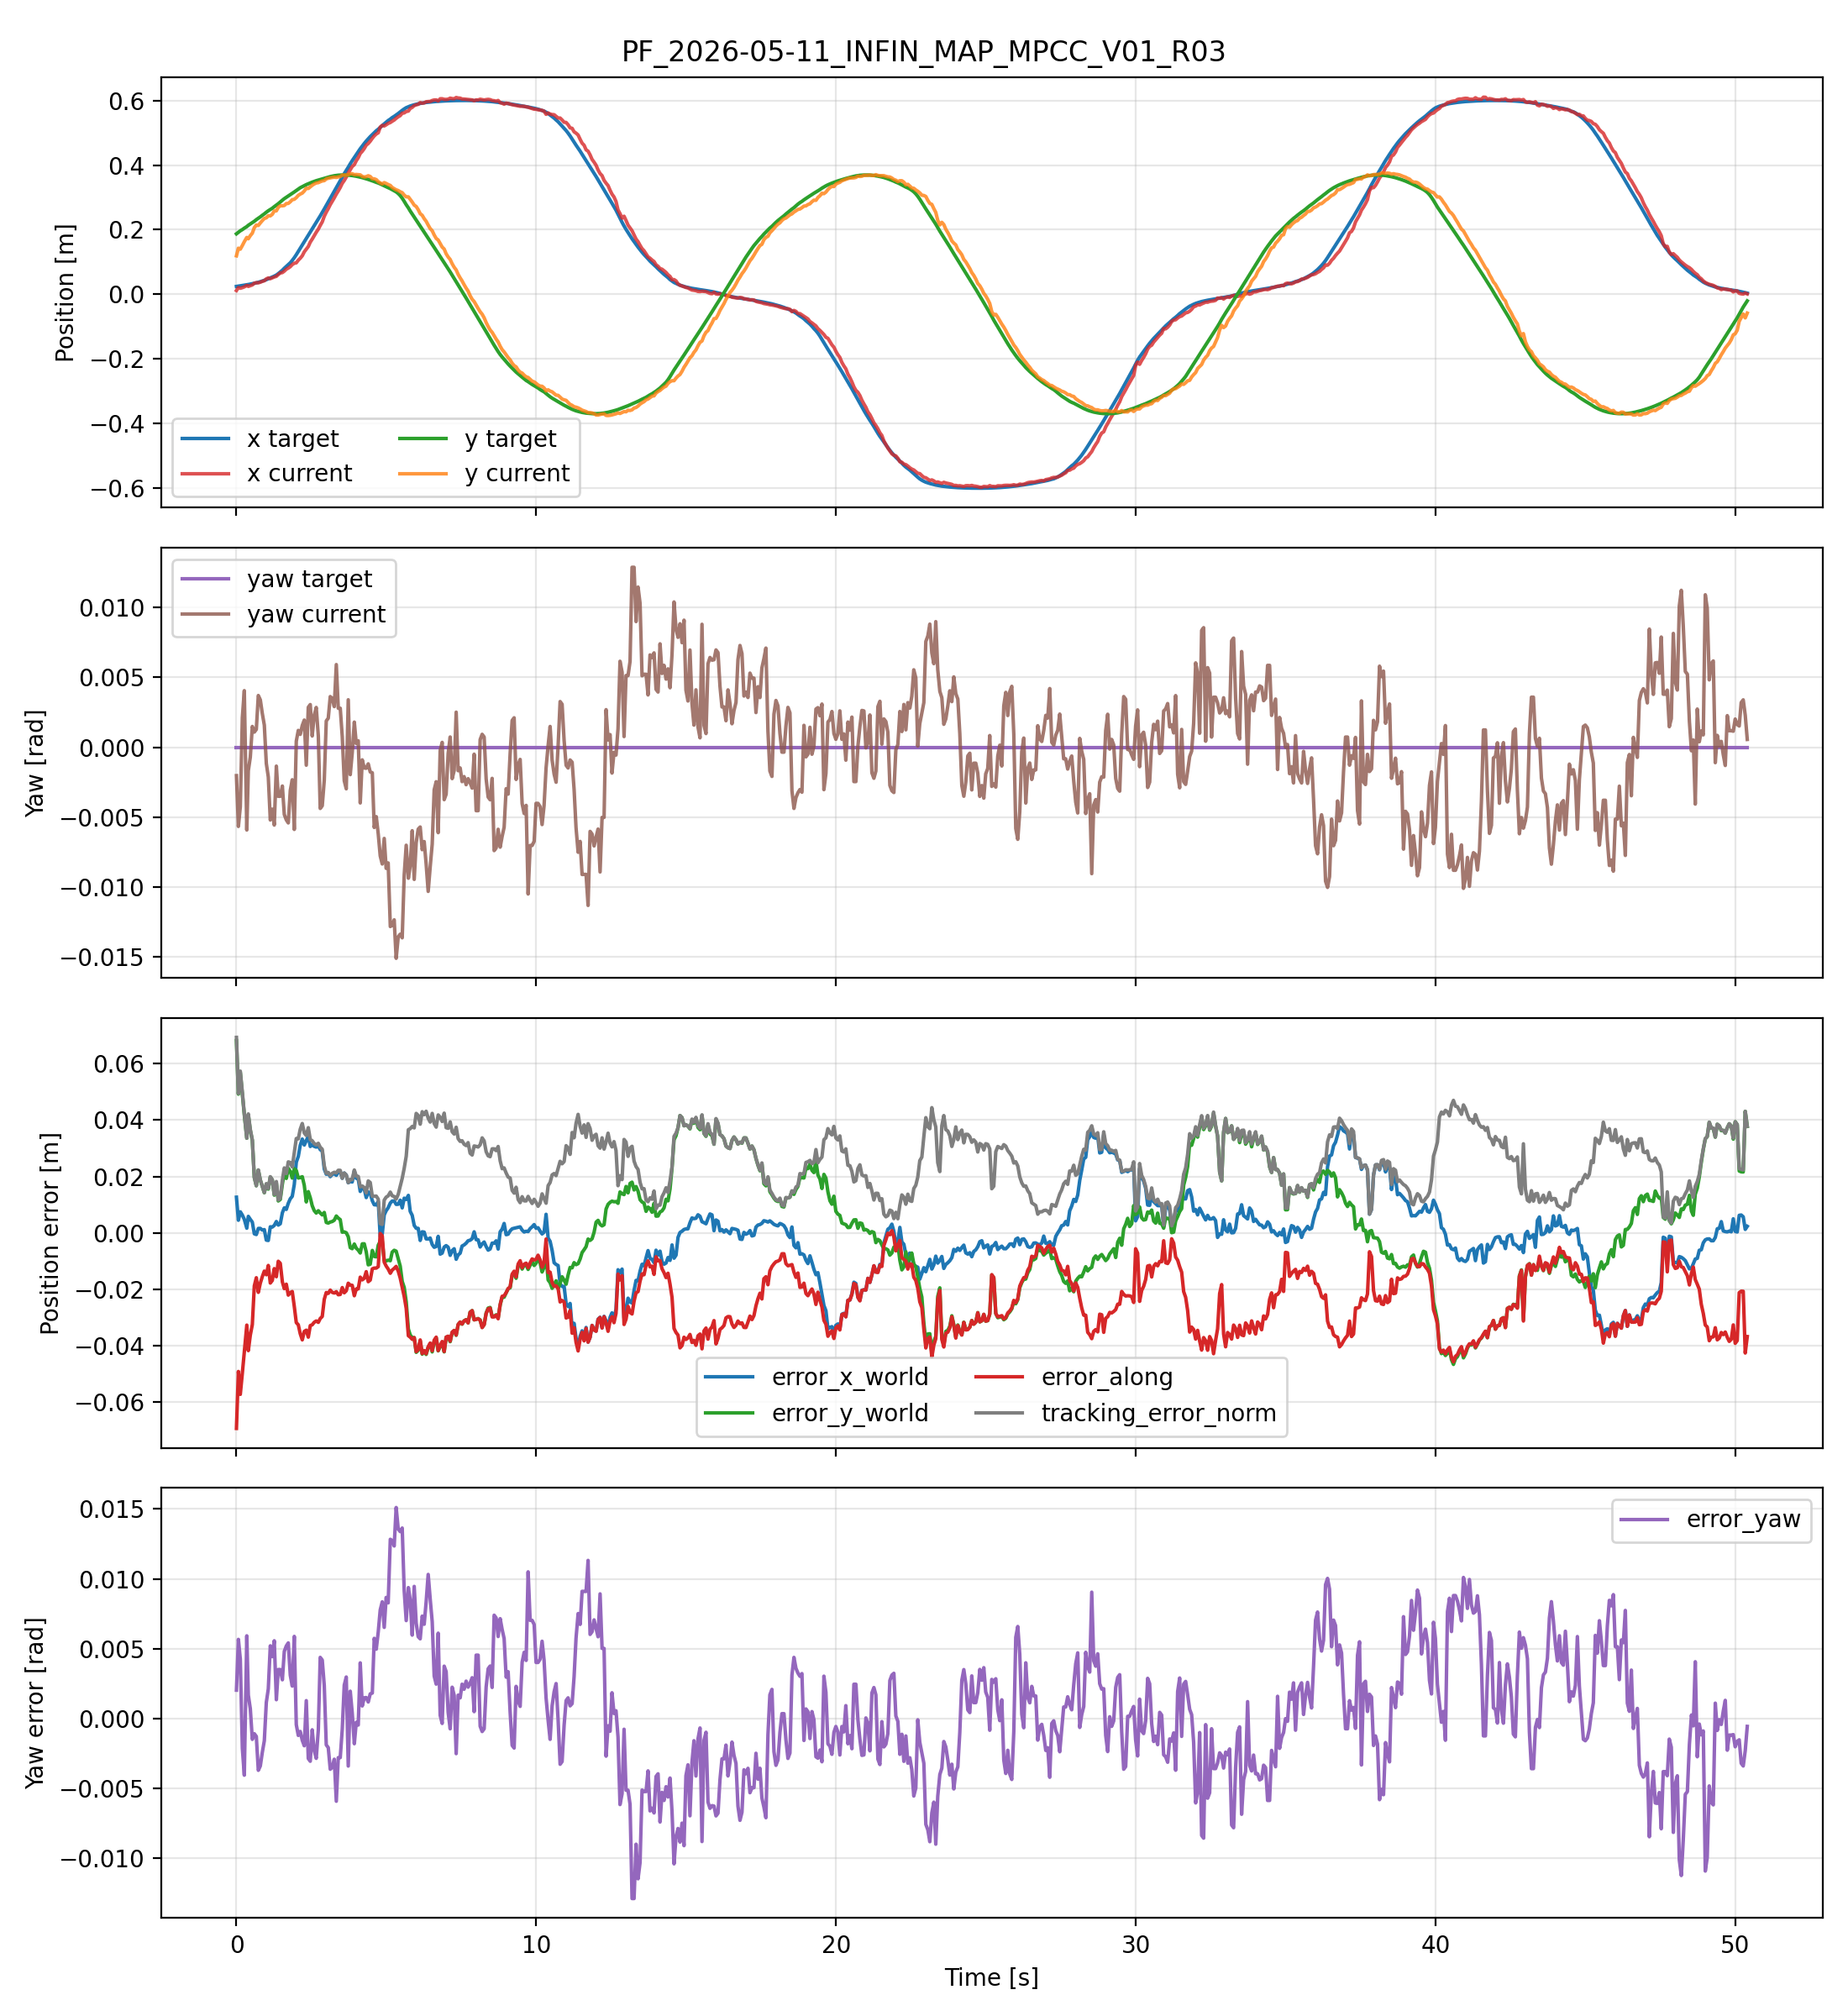
\includegraphics[width=0.7\linewidth]{IMG/controller/MPC/MPC_03_track_error.png}
        \caption{MPC\_03 tracking and errors}
        \label{fig:MPC_03_tracking_and_errors}
    \end{subfigure}
    \caption{Experimental results for MPC\_03 scenario.}
    \label{fig:MPC_03_general}
\end{figure}

\newpage
\begin{figure}[H]
    \centering
    \begin{subfigure}{\textwidth}
        \centering
        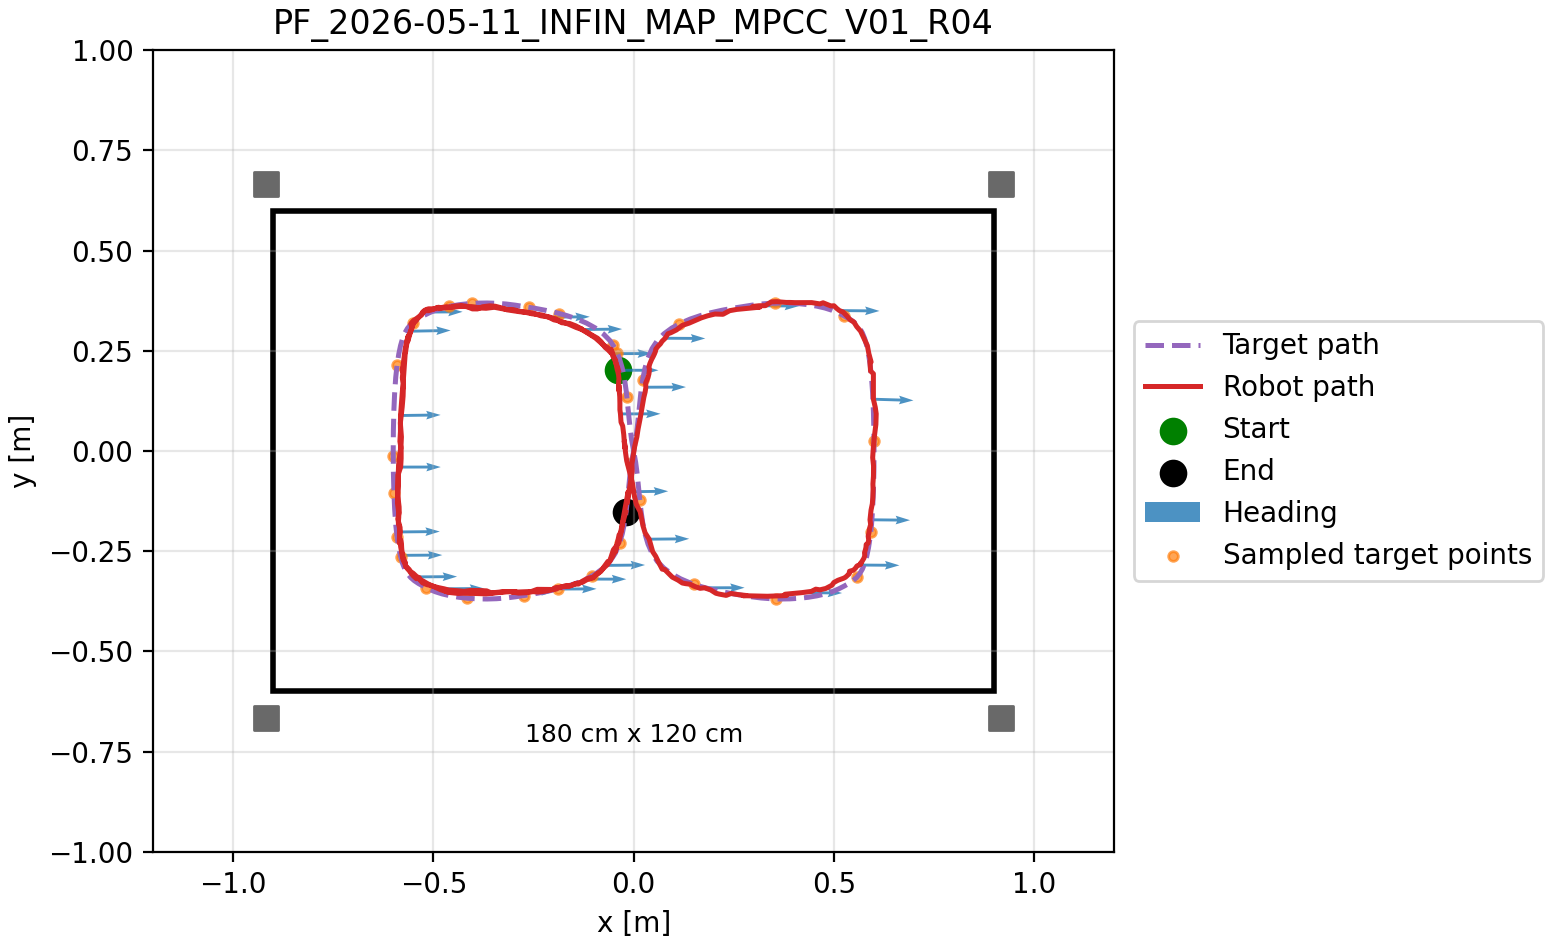
\includegraphics[width=0.7\linewidth]{IMG/controller/MPC/MPC_04_xy_map.png}
        \caption{MPC\_04 xy map}
        \label{fig:MPC_04_xy_map}
    \end{subfigure}

    \vspace{0.5em}

    \begin{subfigure}{\textwidth}
        \centering
        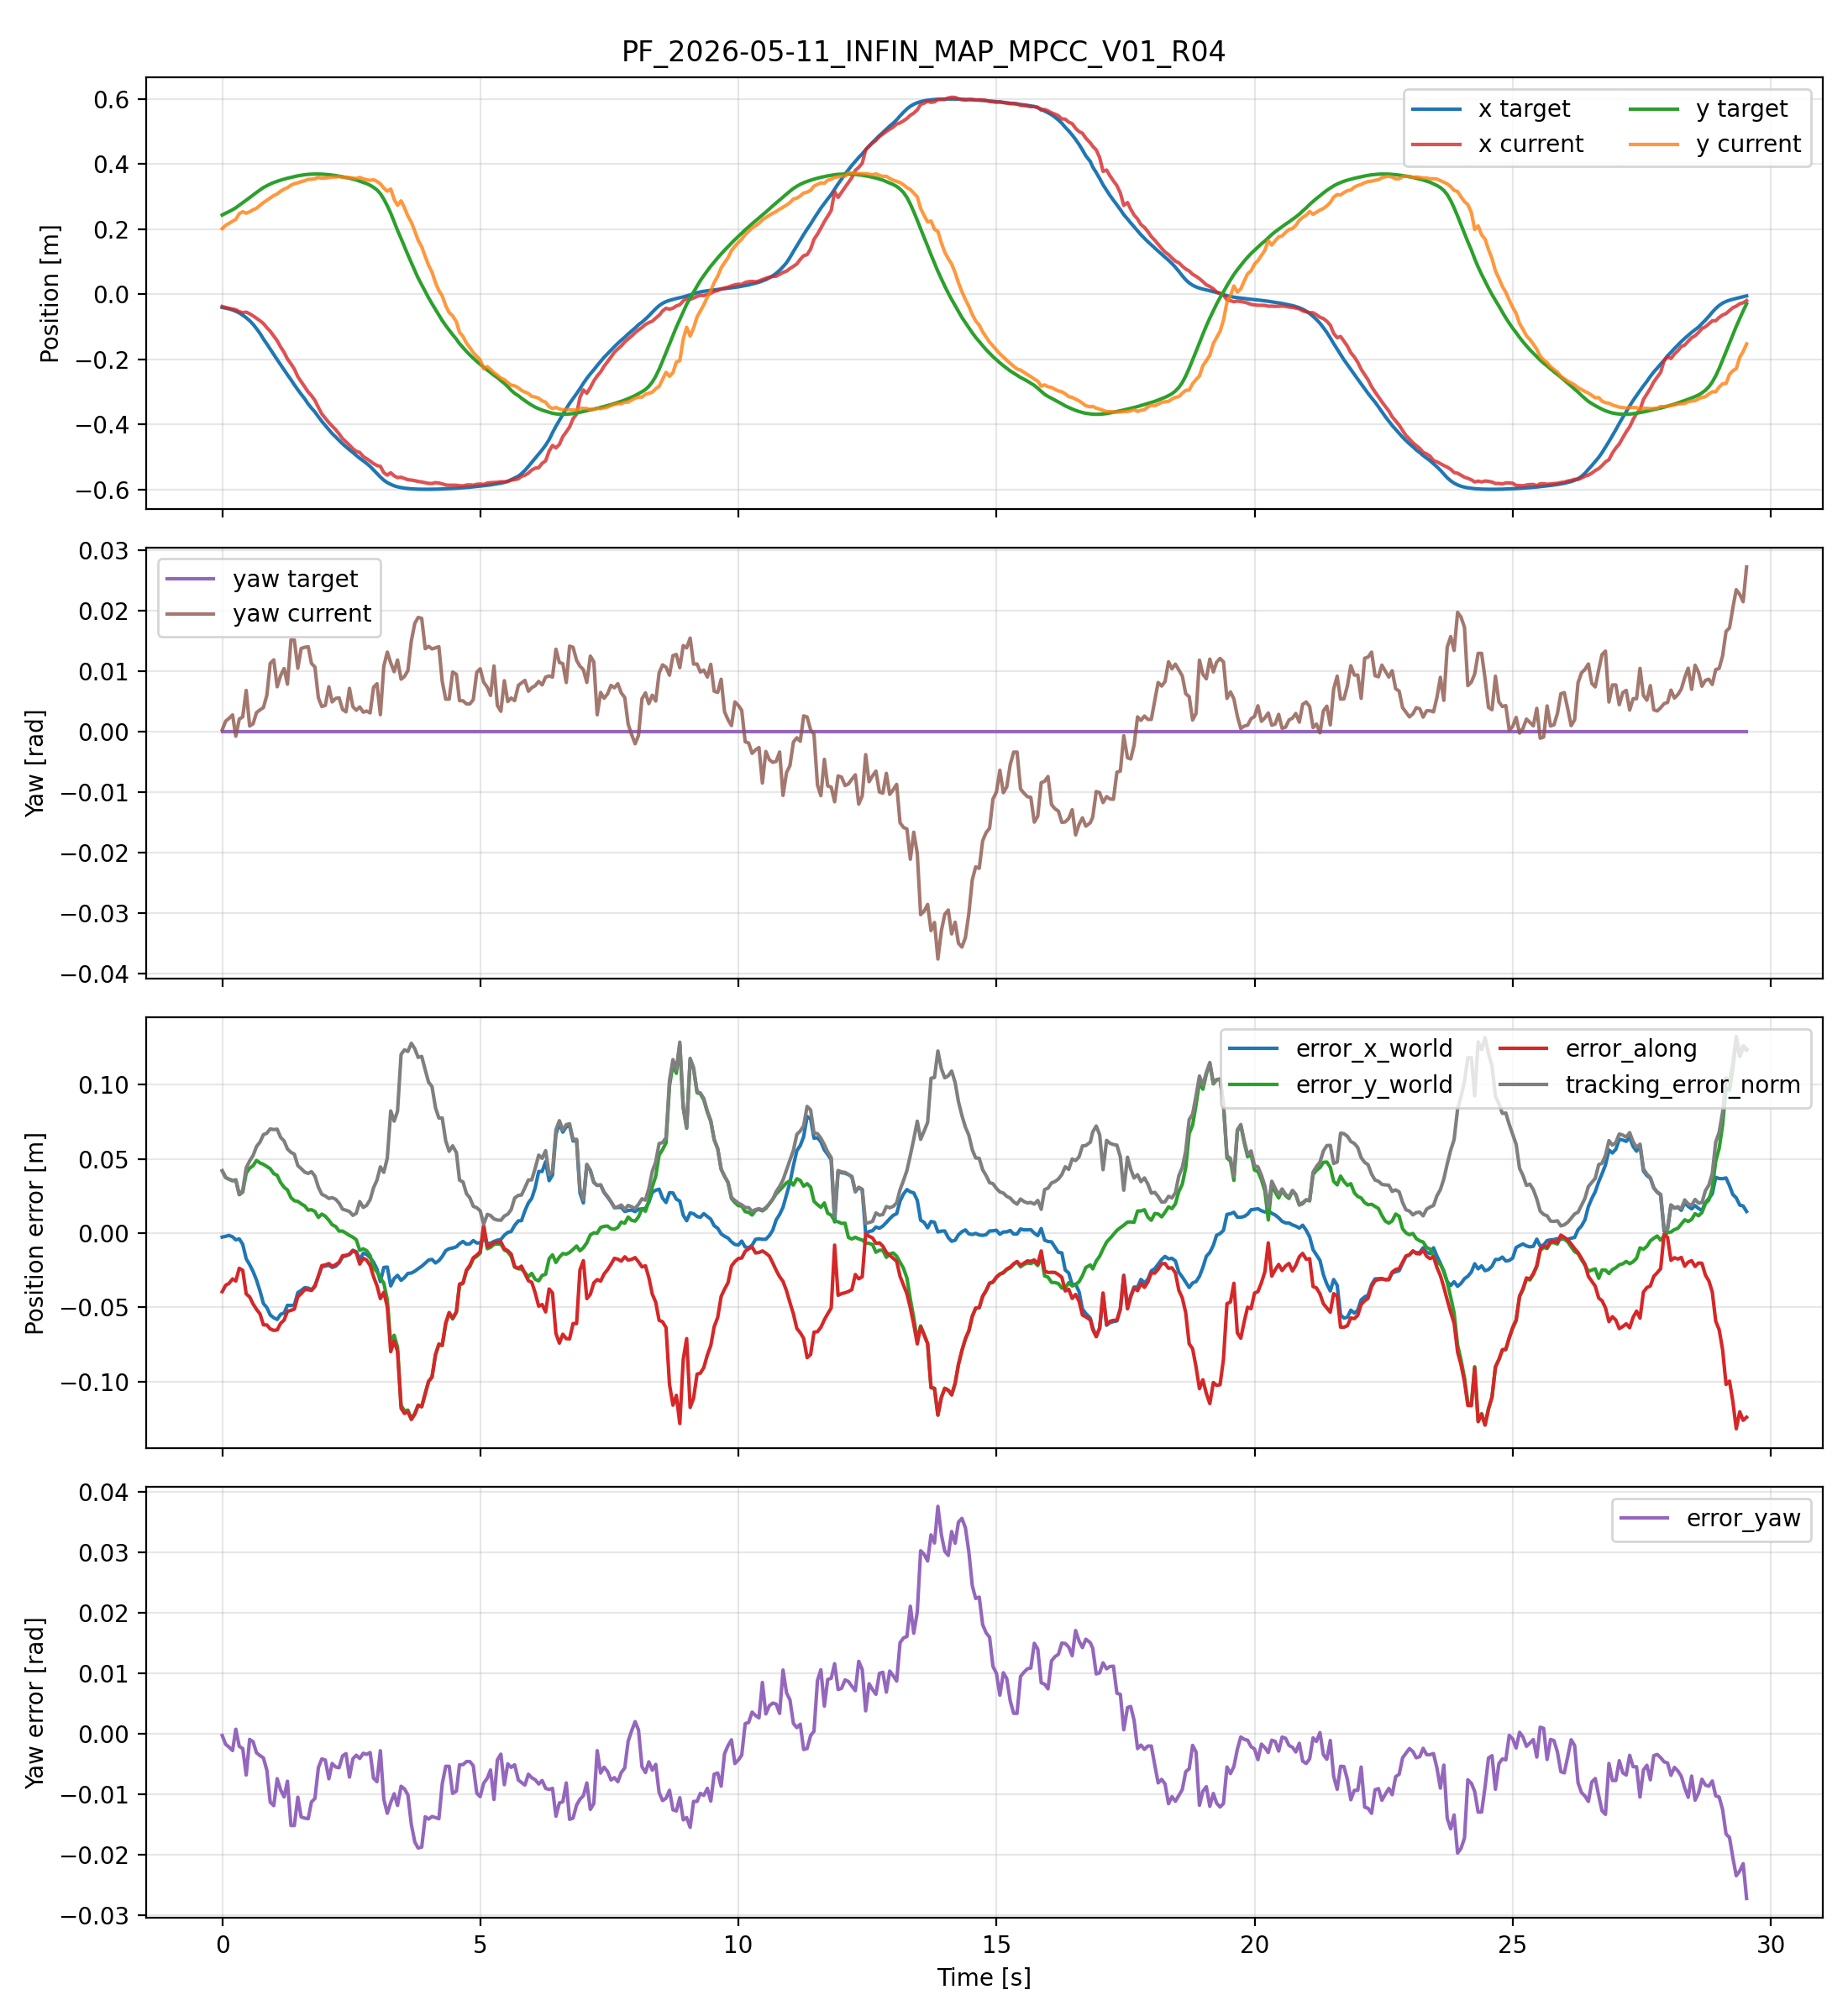
\includegraphics[width=0.7\linewidth]{IMG/controller/MPC/MPC_04_track_error.png}
        \caption{MPC\_04 tracking and errors}
        \label{fig:MPC_04_tracking_and_errors}
    \end{subfigure}
    \caption{Experimental results for MPC\_04 scenario.}
    \label{fig:MPC_04_general}
\end{figure}

\newpage
\begin{figure}[H]
    \centering
    \begin{subfigure}{\textwidth}
        \centering
        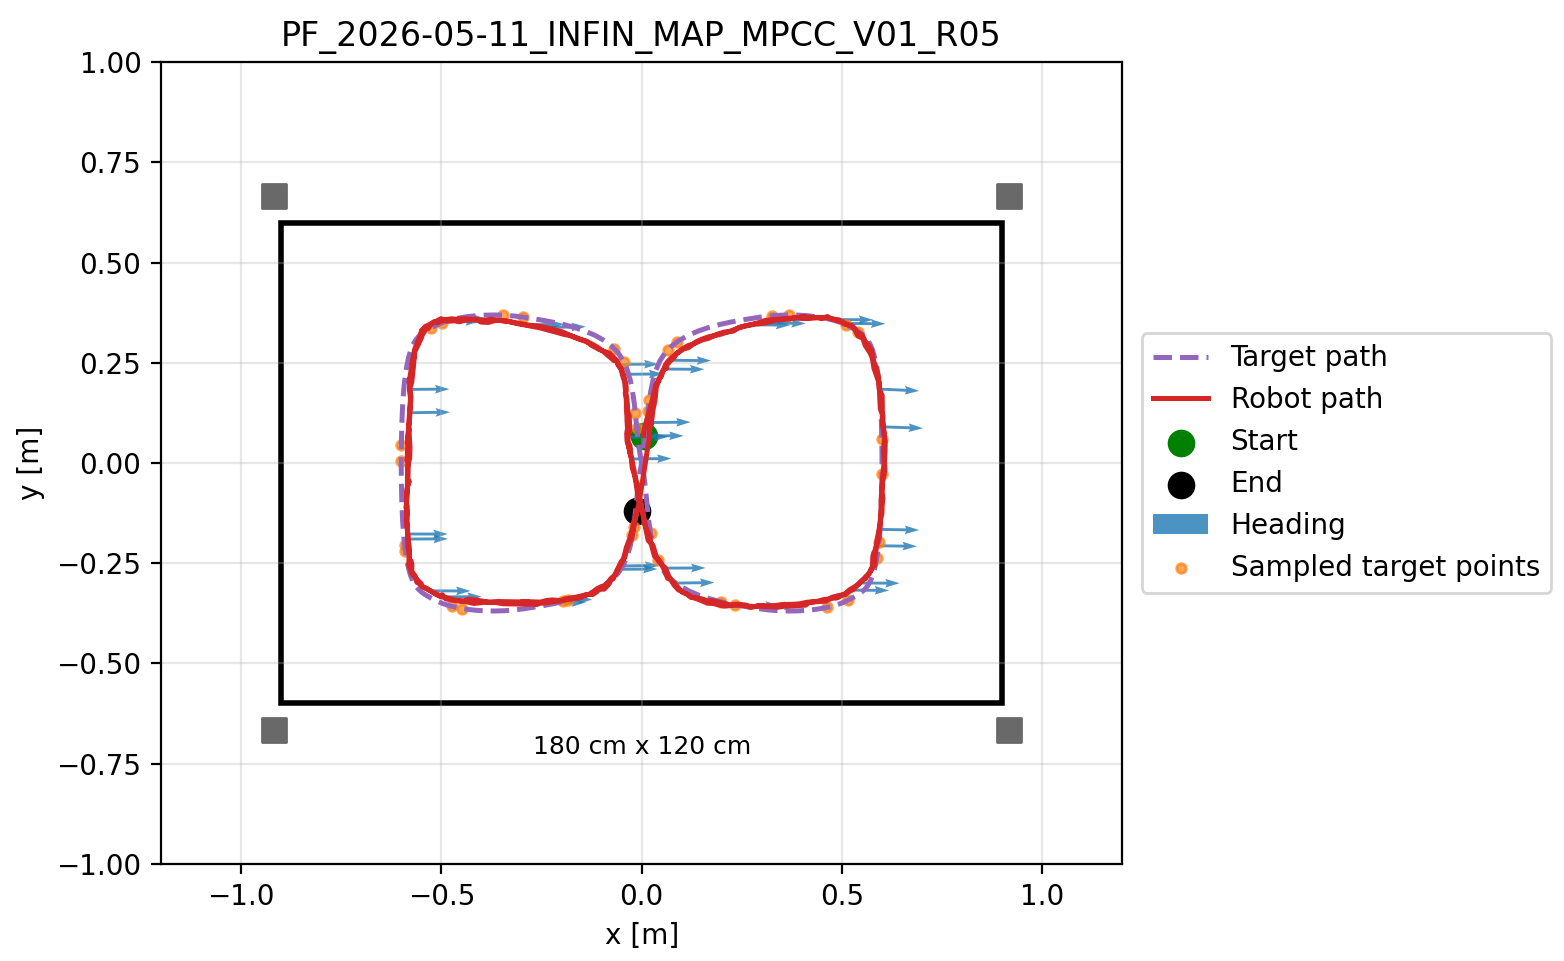
\includegraphics[width=0.7\linewidth]{IMG/controller/MPC/MPC_05_xy_map.png}
        \caption{MPC\_05 xy map}
        \label{fig:MPC_05_xy_map}
    \end{subfigure}

    \vspace{0.5em}

    \begin{subfigure}{\textwidth}
        \centering
        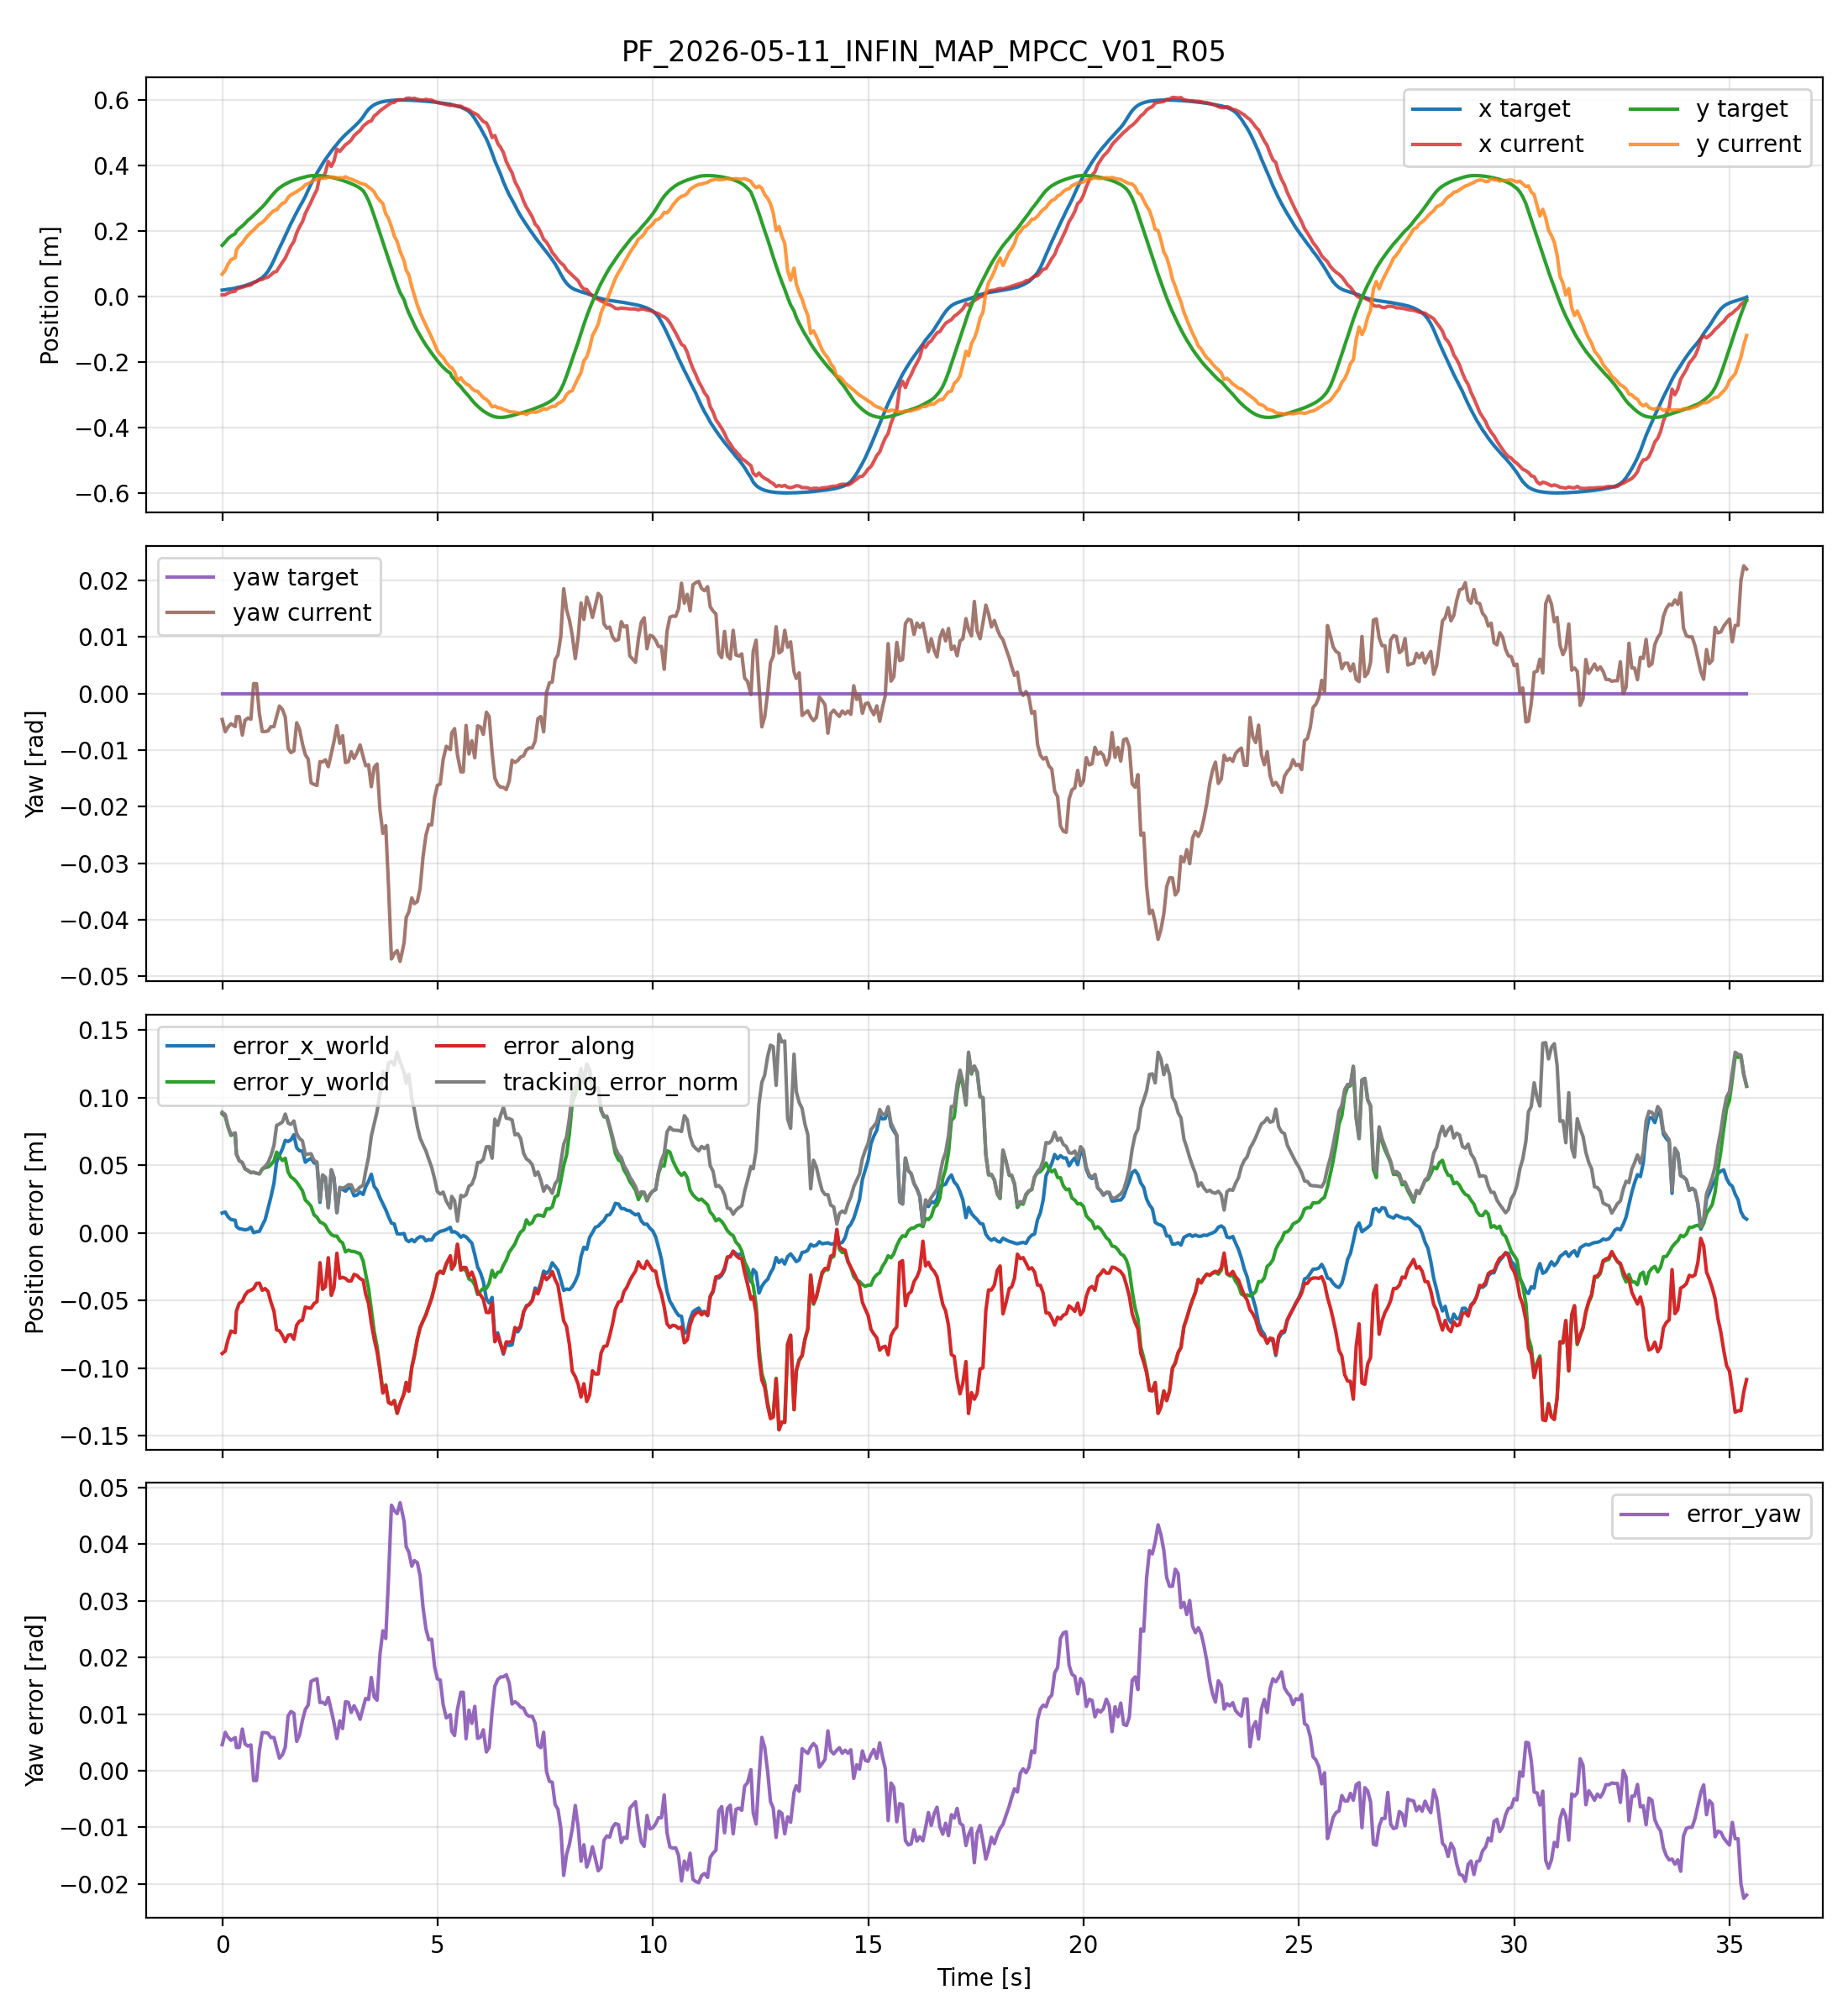
\includegraphics[width=0.7\linewidth]{IMG/controller/MPC/MPC_05_track_error.png}
        \caption{MPC\_05 tracking and errors}
        \label{fig:MPC_05_tracking_and_errors}
    \end{subfigure}
    \caption{Experimental results for MPC\_05 scenario.}
    \label{fig:MPC_05_general}
\end{figure}

\newpage
\begin{figure}[H]
    \centering
    \begin{subfigure}{\textwidth}
        \centering
        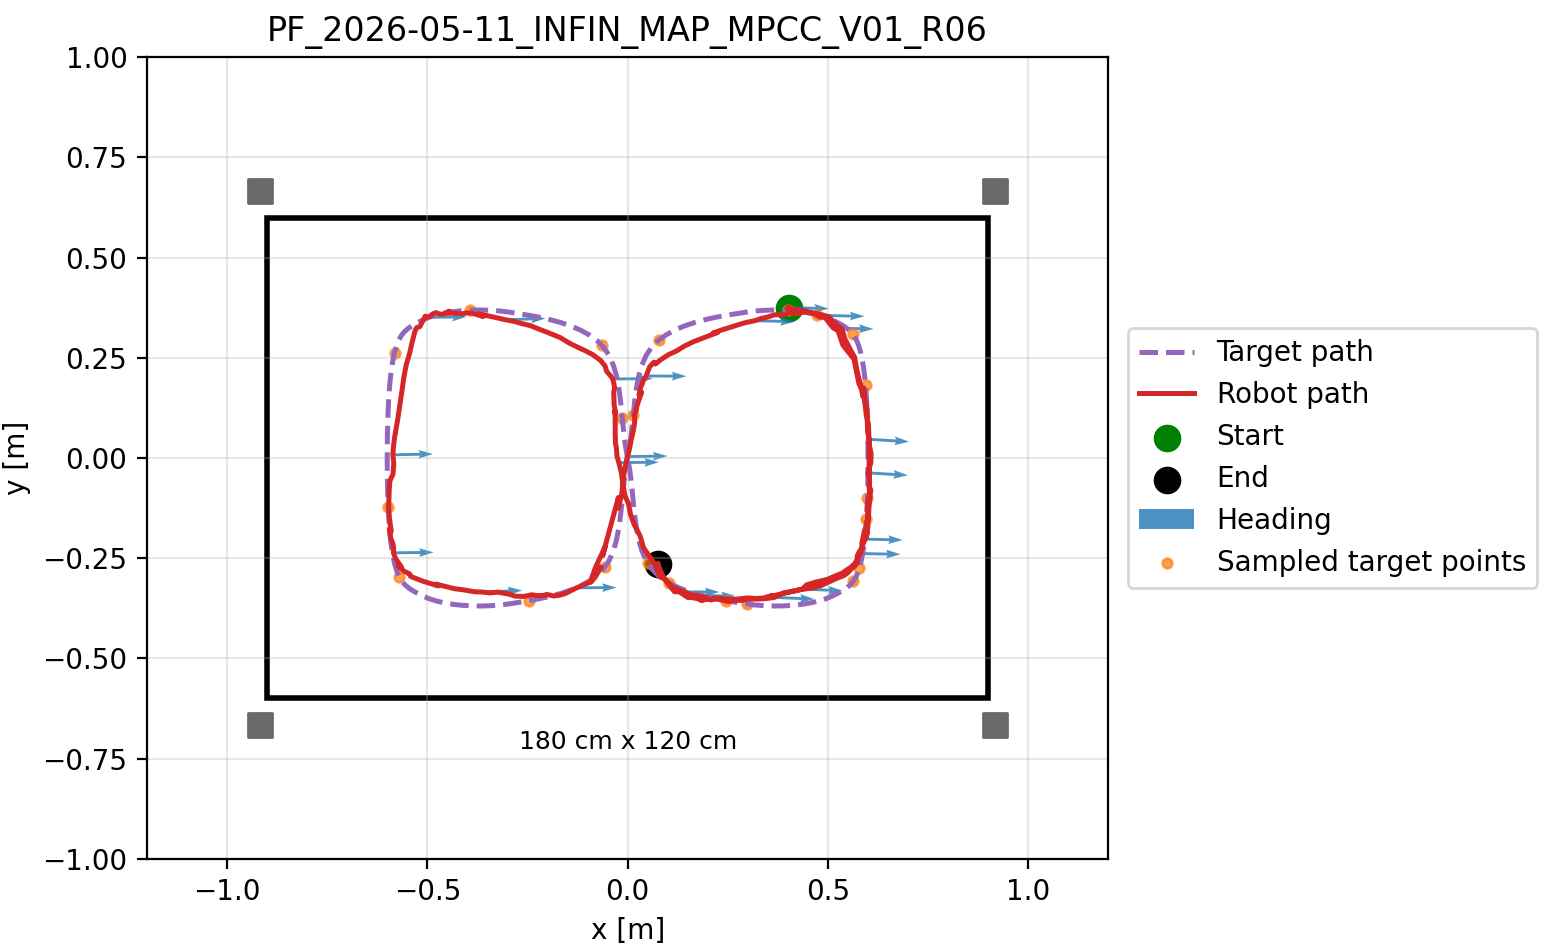
\includegraphics[width=0.7\linewidth]{IMG/controller/MPC/MPC_06_xy_map.png}
        \caption{MPC\_06 xy map}
        \label{fig:MPC_06_xy_map}
    \end{subfigure}

    \vspace{0.5em}

    \begin{subfigure}{\textwidth}
        \centering
        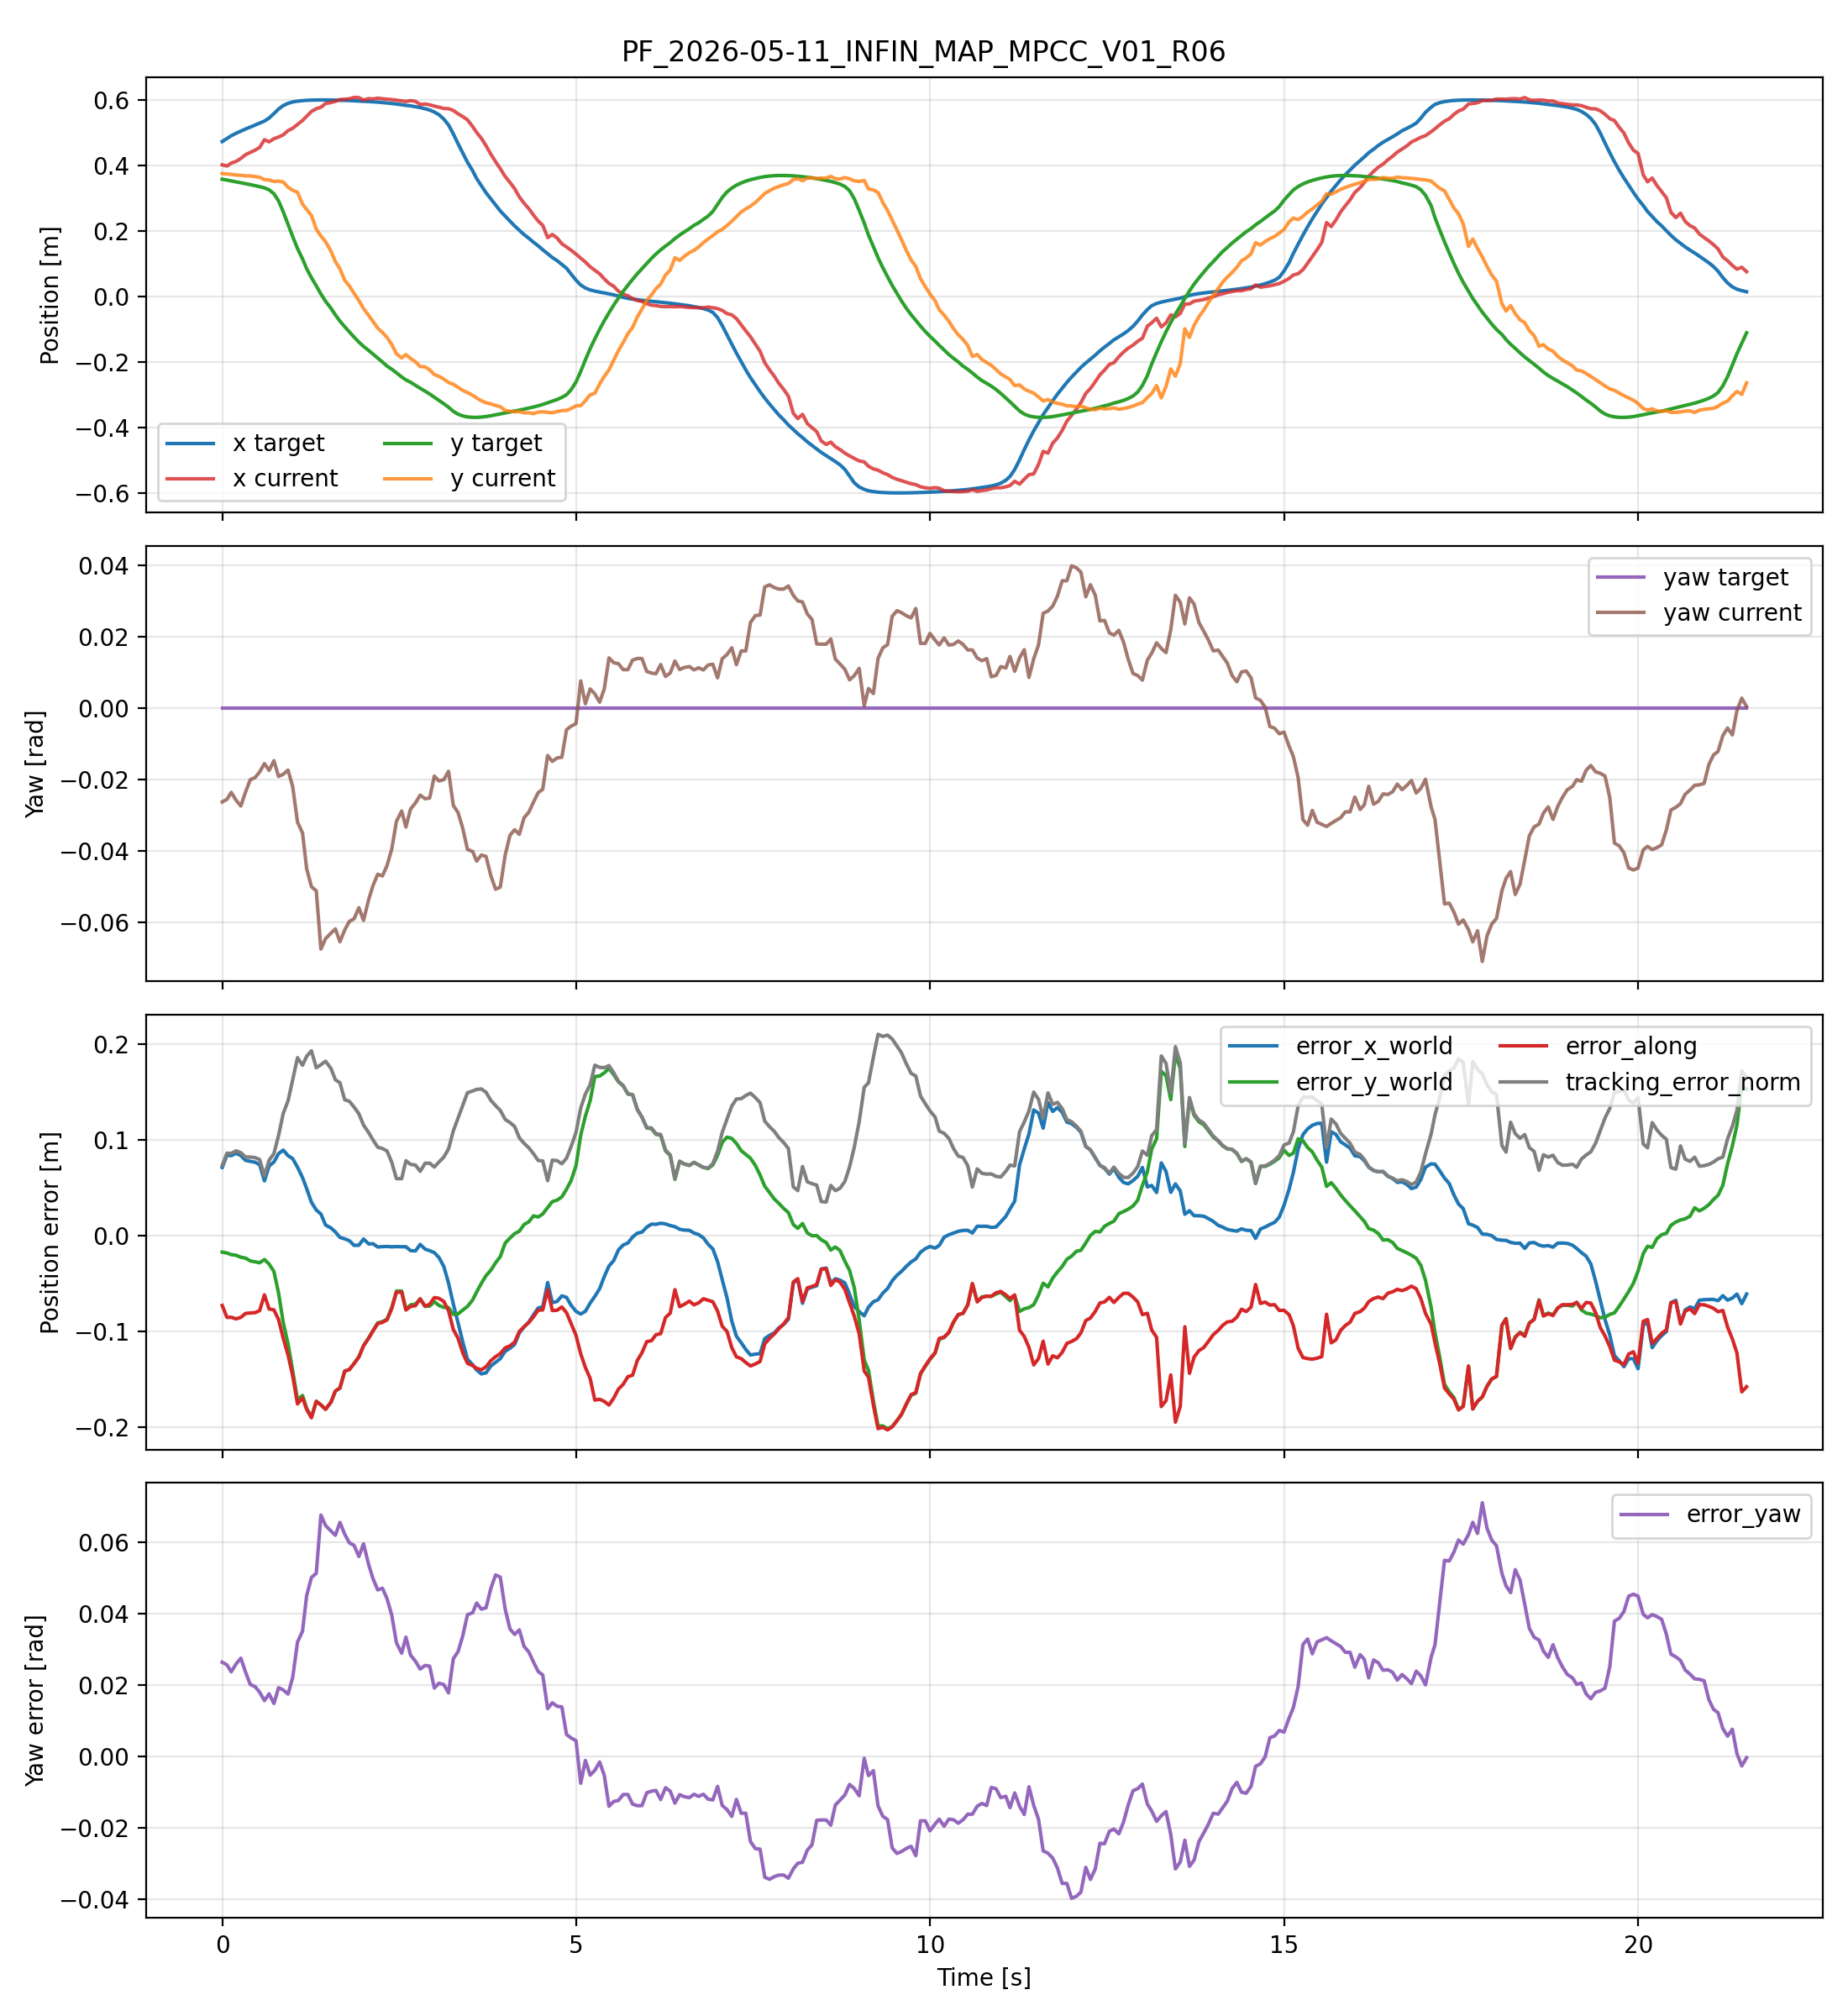
\includegraphics[width=0.7\linewidth]{IMG/controller/MPC/MPC_06_track_error.png}
        \caption{MPC\_06 tracking and errors}
        \label{fig:MPC_06_tracking_and_errors}
    \end{subfigure}
    \caption{Experimental results for MPC\_06 scenario.}
    \label{fig:MPC_06_general}
\end{figure}

\subsection{Comparison Between Linear Segment and MPCC}
  \label{subsec:common_segment_comparison}

  The previous tables evaluate each experiment over its full recorded duration.
  This is useful to understand whether a controller is able to complete the path,
  but it is not always the fairest way to compare tracking quality.  In fact, two
  tests may cover different portions of the infinity-shaped trajectory, and the
  tracking errors computed over the full run may therefore refer to different path
  segments.  For this reason, a final comparison was performed by evaluating each
  pair of tests only over the common portion of the path covered by both runs.

  The comparison was computed using the curvilinear coordinate \(\gamma\).  For a
  set of selected runs, the common interval is defined as:
  \begin{equation}
      \gamma_{\min}^{c}
      =
      \max_j \gamma_{\min,j},
      \qquad
      \gamma_{\max}^{c}
      =
      \min_j \gamma_{\max,j}.
  \end{equation}
  Only the samples satisfying
  \begin{equation}
      \gamma \in
      \left[
          \gamma_{\min}^{c},
          \gamma_{\max}^{c}
      \right]
  \end{equation}
  are used in the final comparison.  This makes the evaluation independent of the
  different total path progress reached by each controller.

  The error is not computed with respect to the internal target point published by
  each controller.  Instead, each measured robot position is compared with the same
  geometric reference path, interpolated at the recorded value of \(\gamma\).  Let
  \(\mathbf{p}=[x\;y]^T\) be the measured robot position and
  \(\mathbf{p}_r(\gamma)=[x_r(\gamma)\;y_r(\gamma)]^T\) the reference point on the
  path.  The position error is:
  \begin{equation}
      \mathbf{e}
      =
      \mathbf{p}
      -
      \mathbf{p}_r(\gamma).
  \end{equation}
  Using the local tangent and normal vectors:
  \begin{equation}
      \mathbf{t}(\gamma)
      =
      \begin{bmatrix}
          \cos\psi_r(\gamma) \\
          \sin\psi_r(\gamma)
      \end{bmatrix},
      \qquad
      \mathbf{n}(\gamma)
      =
      \begin{bmatrix}
          -\sin\psi_r(\gamma) \\
          \cos\psi_r(\gamma)
      \end{bmatrix},
  \end{equation}
  the error is decomposed into lag and contouring components:
  \begin{equation}
      e_l
      =
      \mathbf{e}^T \mathbf{t}(\gamma),
      \qquad
      e_c
      =
      \mathbf{e}^T \mathbf{n}(\gamma).
  \end{equation}
  The contouring error \(e_c\) measures the lateral distance from the path and is
  the most relevant quantity for geometric path-following accuracy.  The lag error
  \(e_l\) measures whether the robot is ahead of or behind the reference point
  along the path direction.  For this final comparison, the reported metrics are:
  \begin{equation}
      \mathrm{RMSE}_{e_c}
      =
      \sqrt{
          \frac{1}{N}
          \sum_{i=1}^{N} e_{c,i}^{2}
      },
      \qquad
      \mathrm{MAE}_{e_c}
      =
      \frac{1}{N}
      \sum_{i=1}^{N} |e_{c,i}|,
  \end{equation}
  \begin{equation}
      \max |e_c|
      =
      \max_{i=1,\dots,N} |e_{c,i}|,
      \qquad
      \mathrm{RMSE}_{e_l}
      =
      \sqrt{
          \frac{1}{N}
          \sum_{i=1}^{N} e_{l,i}^{2}
      },
      \qquad
      \mathrm{MAE}_{e_l}
      =
      \frac{1}{N}
      \sum_{i=1}^{N} |e_{l,i}|.
  \end{equation}
  The path progress ratio and the velocity saturation ratios are not included in
this final comparison, because the objective here is to isolate the tracking
quality on the same path segment.

\begin{table}[H]
\centering
\caption{Common-segment comparison between selected Linear Segment and MPCC
tests.}
\label{tab:common_segment_comparison}
\scriptsize
\setlength{\tabcolsep}{3pt}
\renewcommand{\arraystretch}{1.05}
\begin{tabular}{lccccccc}
\toprule
\textbf{Run} &
\shortstack{\textbf{Common}\\\textbf{segment [m]}} &
\textbf{Duration [s]} &
\(\mathrm{RMSE}_{e_c}\) [m] &
\(\mathrm{MAE}_{e_c}\) [m] &
\(\max |e_c|\) [m] &
\(\mathrm{RMSE}_{e_l}\) [m] &
\(\mathrm{MAE}_{e_l}\) [m] \\
\midrule
LIN-04 & 4.548 & 50.14 & 0.0115 & 0.0086 & 0.0367 & 0.0003 & 0.0002 \\
LIN-05 & 4.548 & 38.86 & 0.0259 & 0.0210 & 0.0646 & 0.0010 & 0.0005 \\
\midrule
MPC-05 & 4.534 & 35.39 & 0.0170 & 0.0144 & 0.0357 & 0.0666 & 0.0587 \\
MPC-06 & 4.534 & 21.53 & 0.0330 & 0.0257 & 0.0705 & 0.1105 & 0.1039 \\
\midrule
LIN-05 & 4.534 & 22.58 & 0.0469 & 0.0391 & 0.1166 & 0.0011 & 0.0006 \\
MPC-06 & 4.534 & 21.53 & 0.0330 & 0.0257 & 0.0705 & 0.1105 & 0.1039 \\
\bottomrule
\end{tabular}
\end{table}

The first comparison considers two Linear Segment runs. The slower configuration
LIN-R05 achieves the best contouring performance. Increasing the velocity in
LIN-R06 reduces the duration from \(50.14~\mathrm{s}\) to
\(38.86~\mathrm{s}\), but the maximum contouring error increases from
\(0.0367~\mathrm{m}\) to \(0.0646~\mathrm{m}\), which is almost doubled.
This confirms that the Linear Segment controller is very accurate at moderate
speed, but its lateral tracking quality degrades as the motion becomes more
aggressive.

The second comparison considers two MPCC runs. MPC-R05 provides better geometric
tracking, with \(\mathrm{RMSE}_{e_c}=0.0170~\mathrm{m}\) and
\(\max |e_c|=0.0357~\mathrm{m}\). MPC-R06 is faster, completing the common
segment in \(21.53~\mathrm{s}\), but the contouring error increases to
\(\mathrm{RMSE}_{e_c}=0.0330~\mathrm{m}\), with a maximum contouring error of
\(0.0705~\mathrm{m}\). The lag error also increases significantly, from
\(\mathrm{RMSE}_{e_l}=0.0666~\mathrm{m}\) to
\(\mathrm{RMSE}_{e_l}=0.1105~\mathrm{m}\). This indicates that the aggressive
MPCC configuration favours path advancement, but introduces a larger mismatch
between the robot motion and the virtual path coordinate.

The final cross-comparison evaluates the aggressive Linear Segment run LIN-R10
against MPC-R06 over the same \(4.534~\mathrm{m}\) common segment. In this case,
MPC-R06 achieves better lateral path-following accuracy:
\[
    \mathrm{RMSE}_{e_c}
    =
    0.0330~\mathrm{m}
    \quad \text{against} \quad
    0.0469~\mathrm{m}
\]
for LIN-R10. The maximum contouring error is also lower for MPC-R06:
\[
    \max |e_c|
    =
    0.0705~\mathrm{m}
    \quad \text{against} \quad
    0.1166~\mathrm{m}.
\]
However, the lag error remains much larger for MPC-R06
\((\mathrm{RMSE}_{e_l}=0.1105~\mathrm{m})\) than for the Linear Segment
controller \((\mathrm{RMSE}_{e_l}=0.0011~\mathrm{m})\). Therefore, the MPCC
shows better lateral geometric tracking in the aggressive comparison, but still
requires further tuning of the lag penalty and path advancement dynamics. The
Linear Segment controller remains simpler and very effective when its velocity
is moderate, while the MPCC becomes more promising when higher-speed geometric
path following is required.

  \begin{figure}[H]
      \centering
      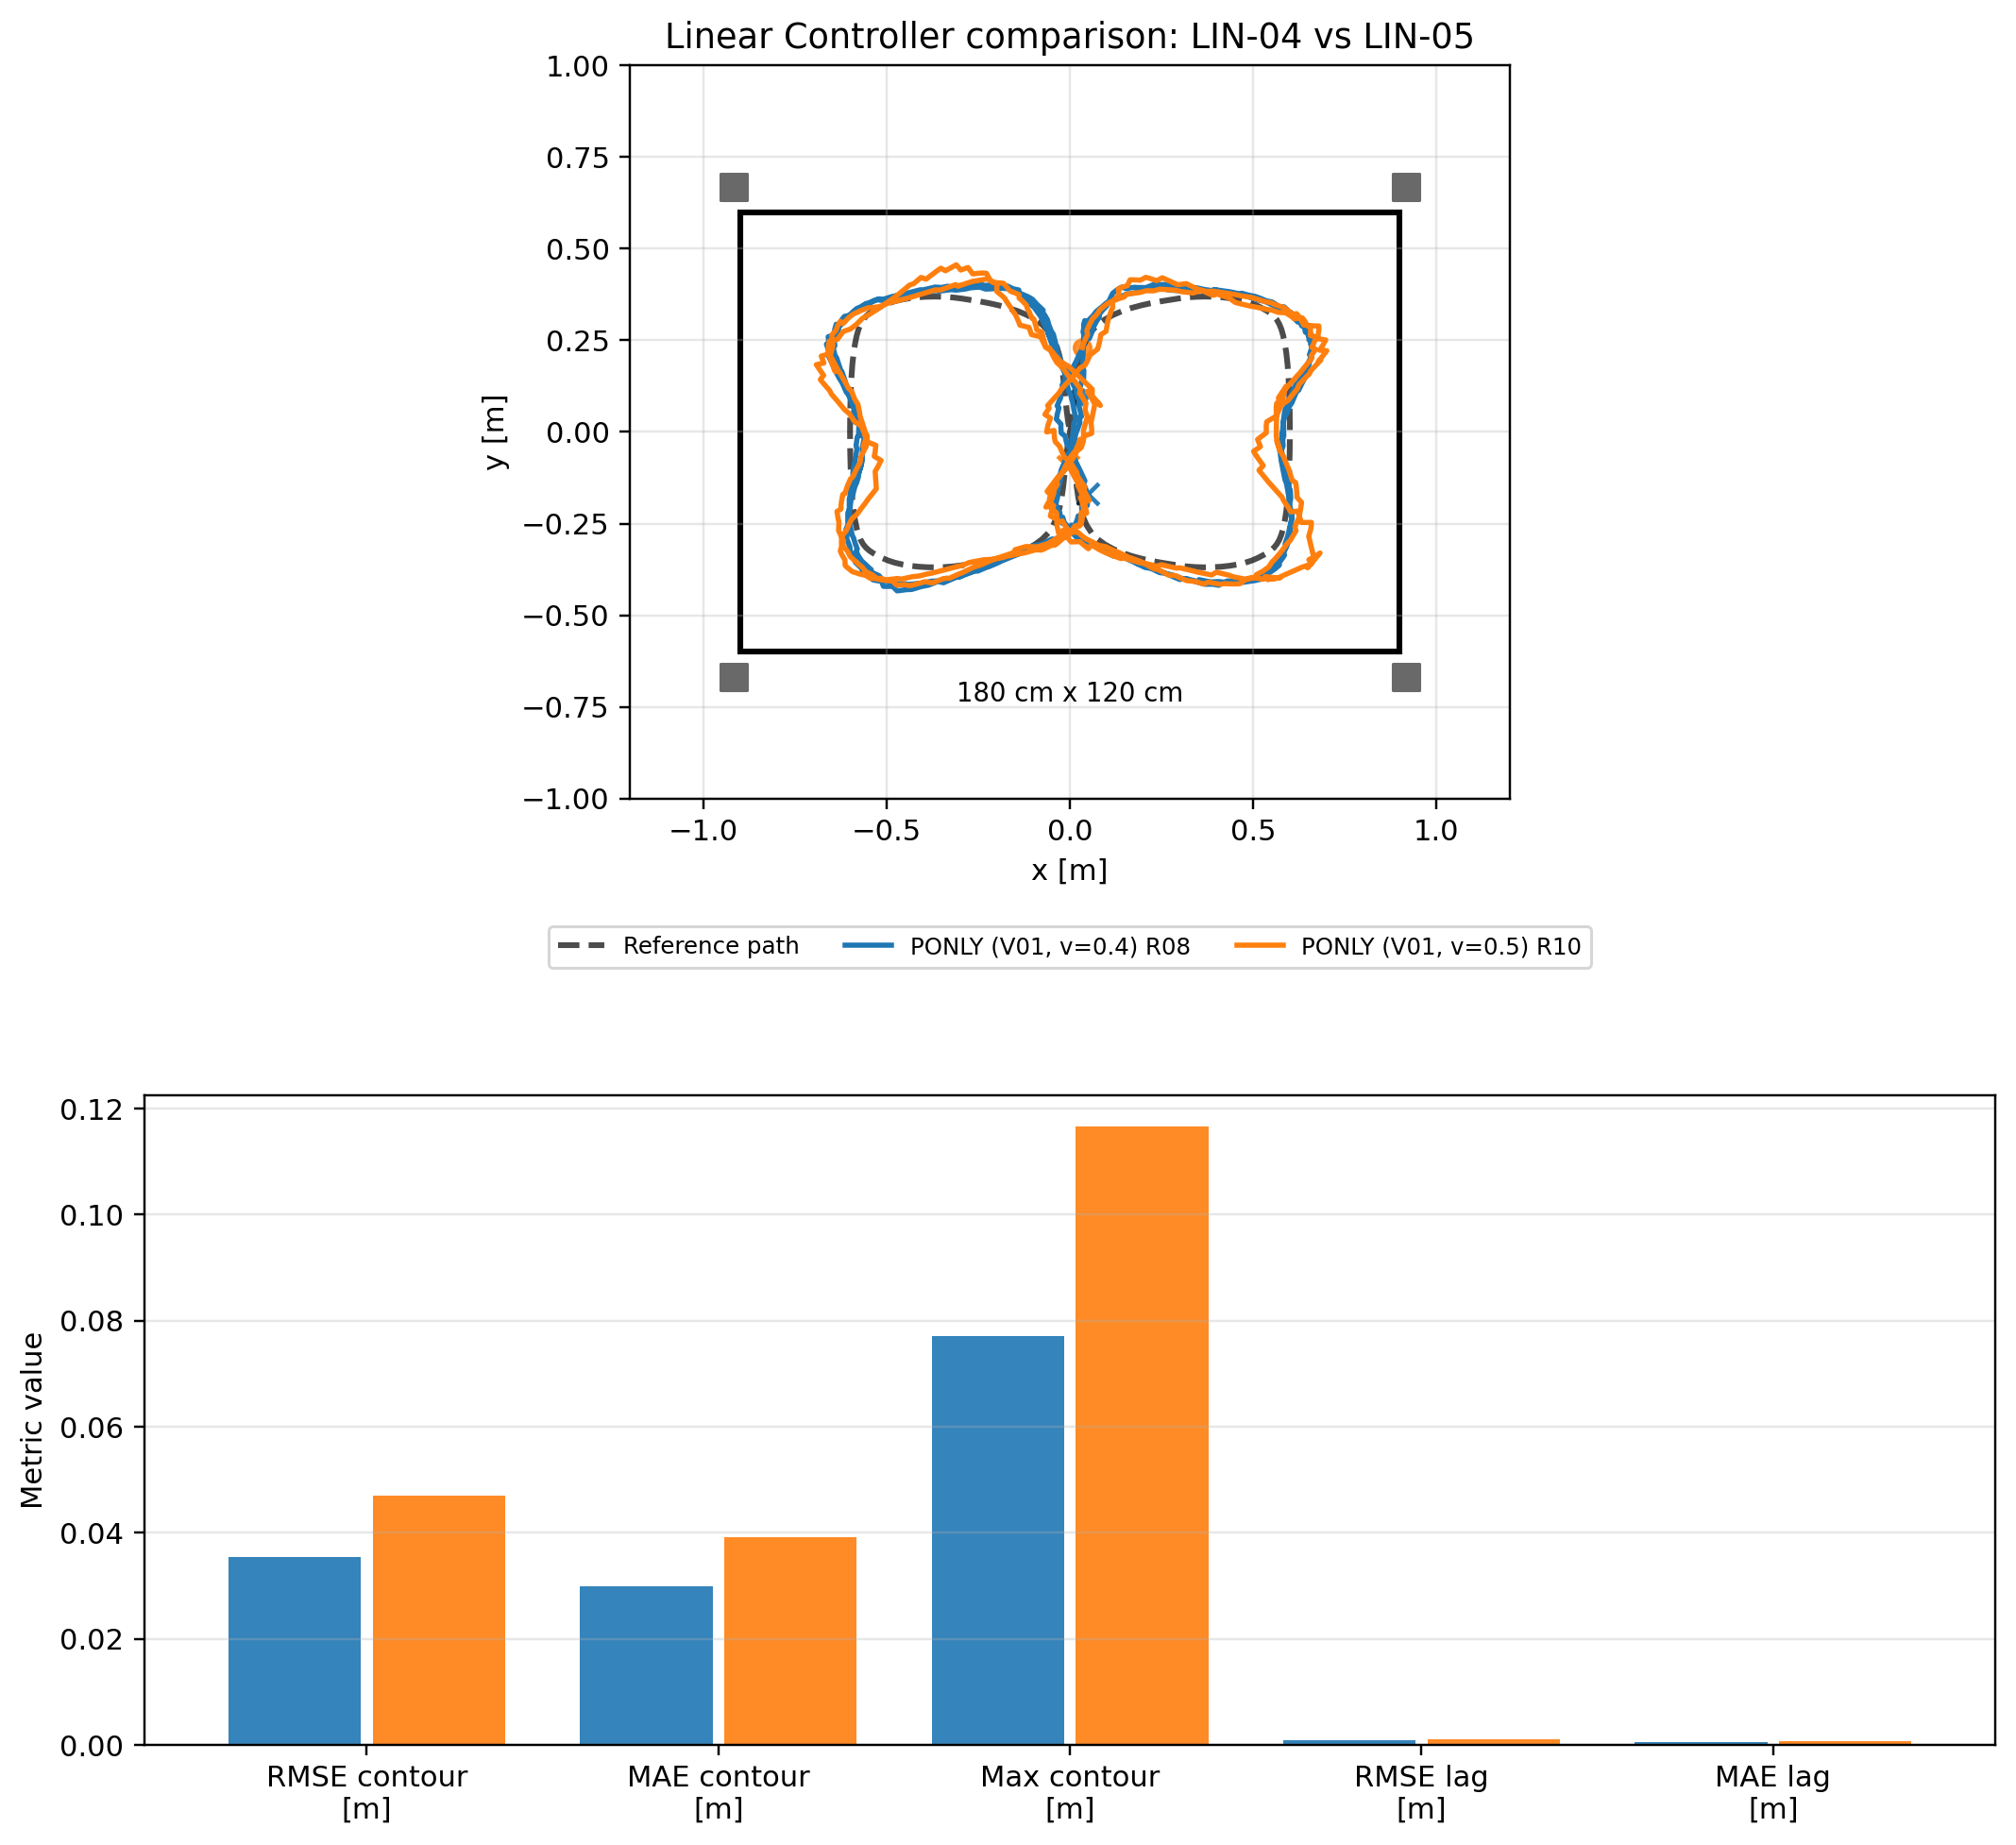
\includegraphics[width=0.95\linewidth]{IMG/controller/COMPARISON/compare_LIN05_LIN06.png}
      \caption{Common-segment comparison between two Linear Segment runs.  The
  upper plot shows the overlapped \(xy\) trajectories, while the lower plot reports
  the contouring and lag error metrics.}
      \label{fig:compare_lin05_lin06}
  \end{figure}

  \begin{figure}[H]
      \centering
      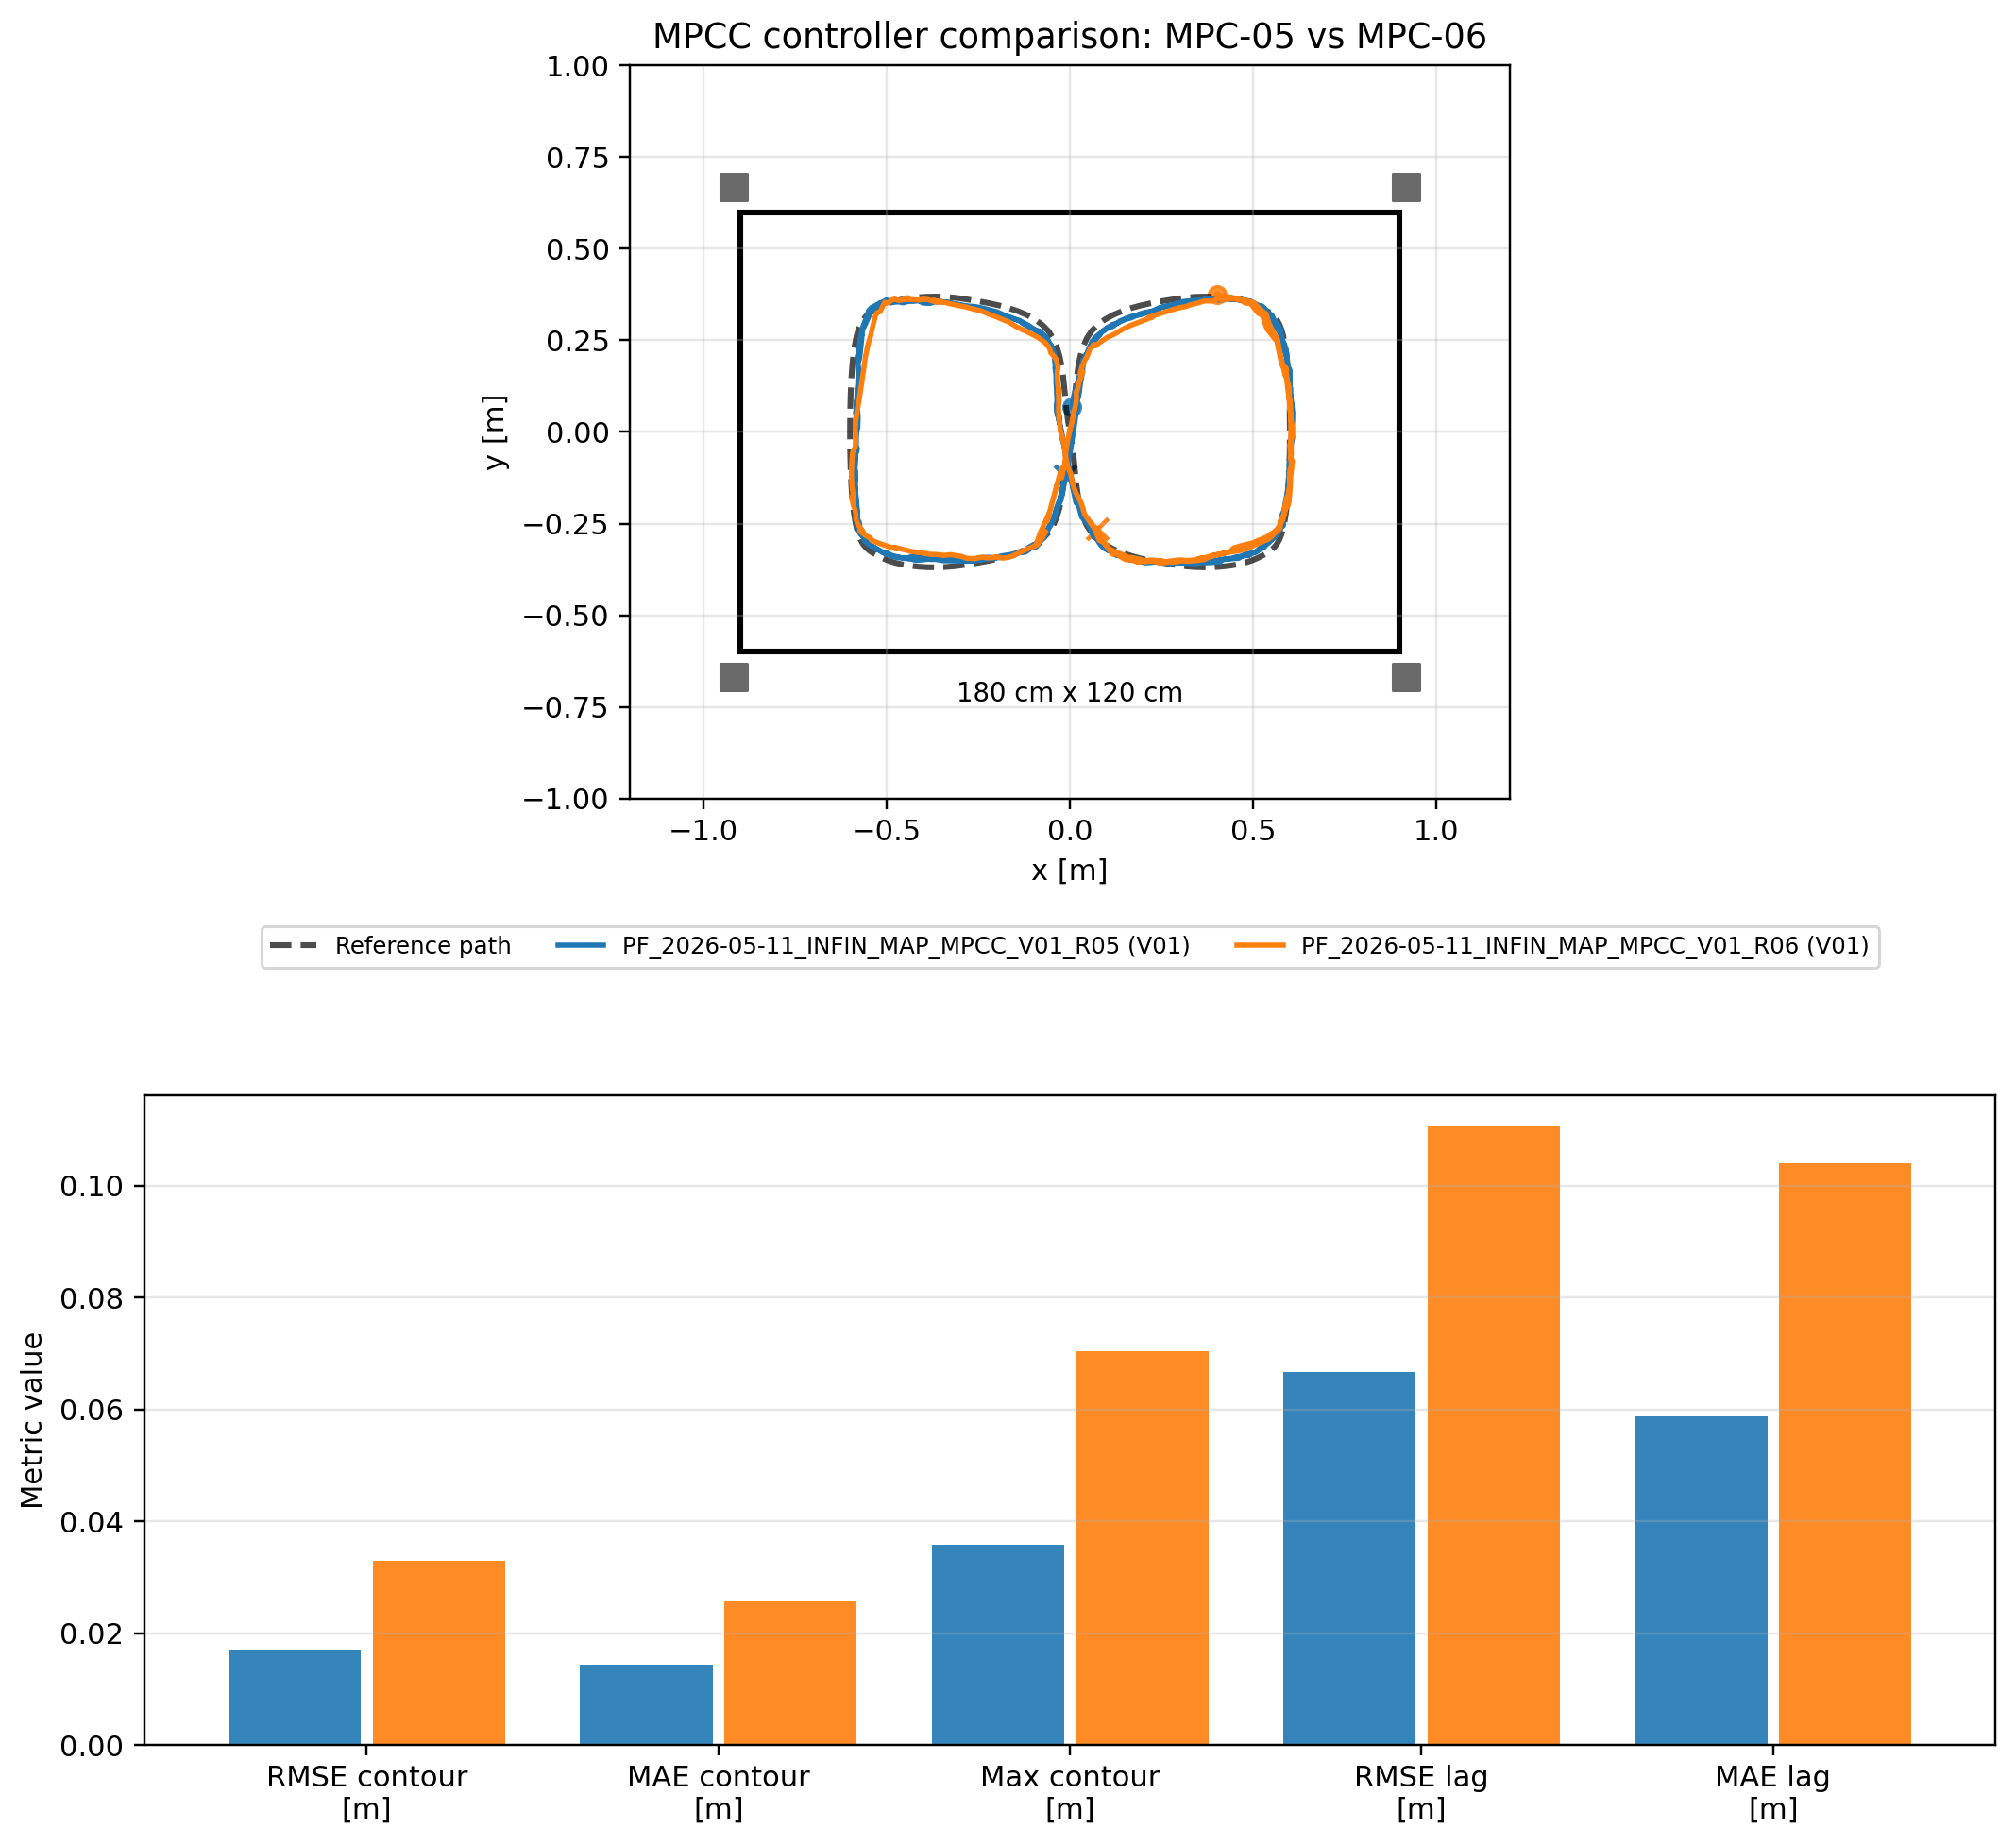
\includegraphics[width=0.95\linewidth]{IMG/controller/COMPARISON/compare_MPC05_MPC06.png}
      \caption{Common-segment comparison between two MPCC runs.  The figure
  highlights the loss of contouring accuracy and the increase in lag error when
  moving from MPC-05 to the more aggressive MPC-06 configuration.}
      \label{fig:compare_mpc05_mpc06}
  \end{figure}

\begin{figure}[H]
    \centering
    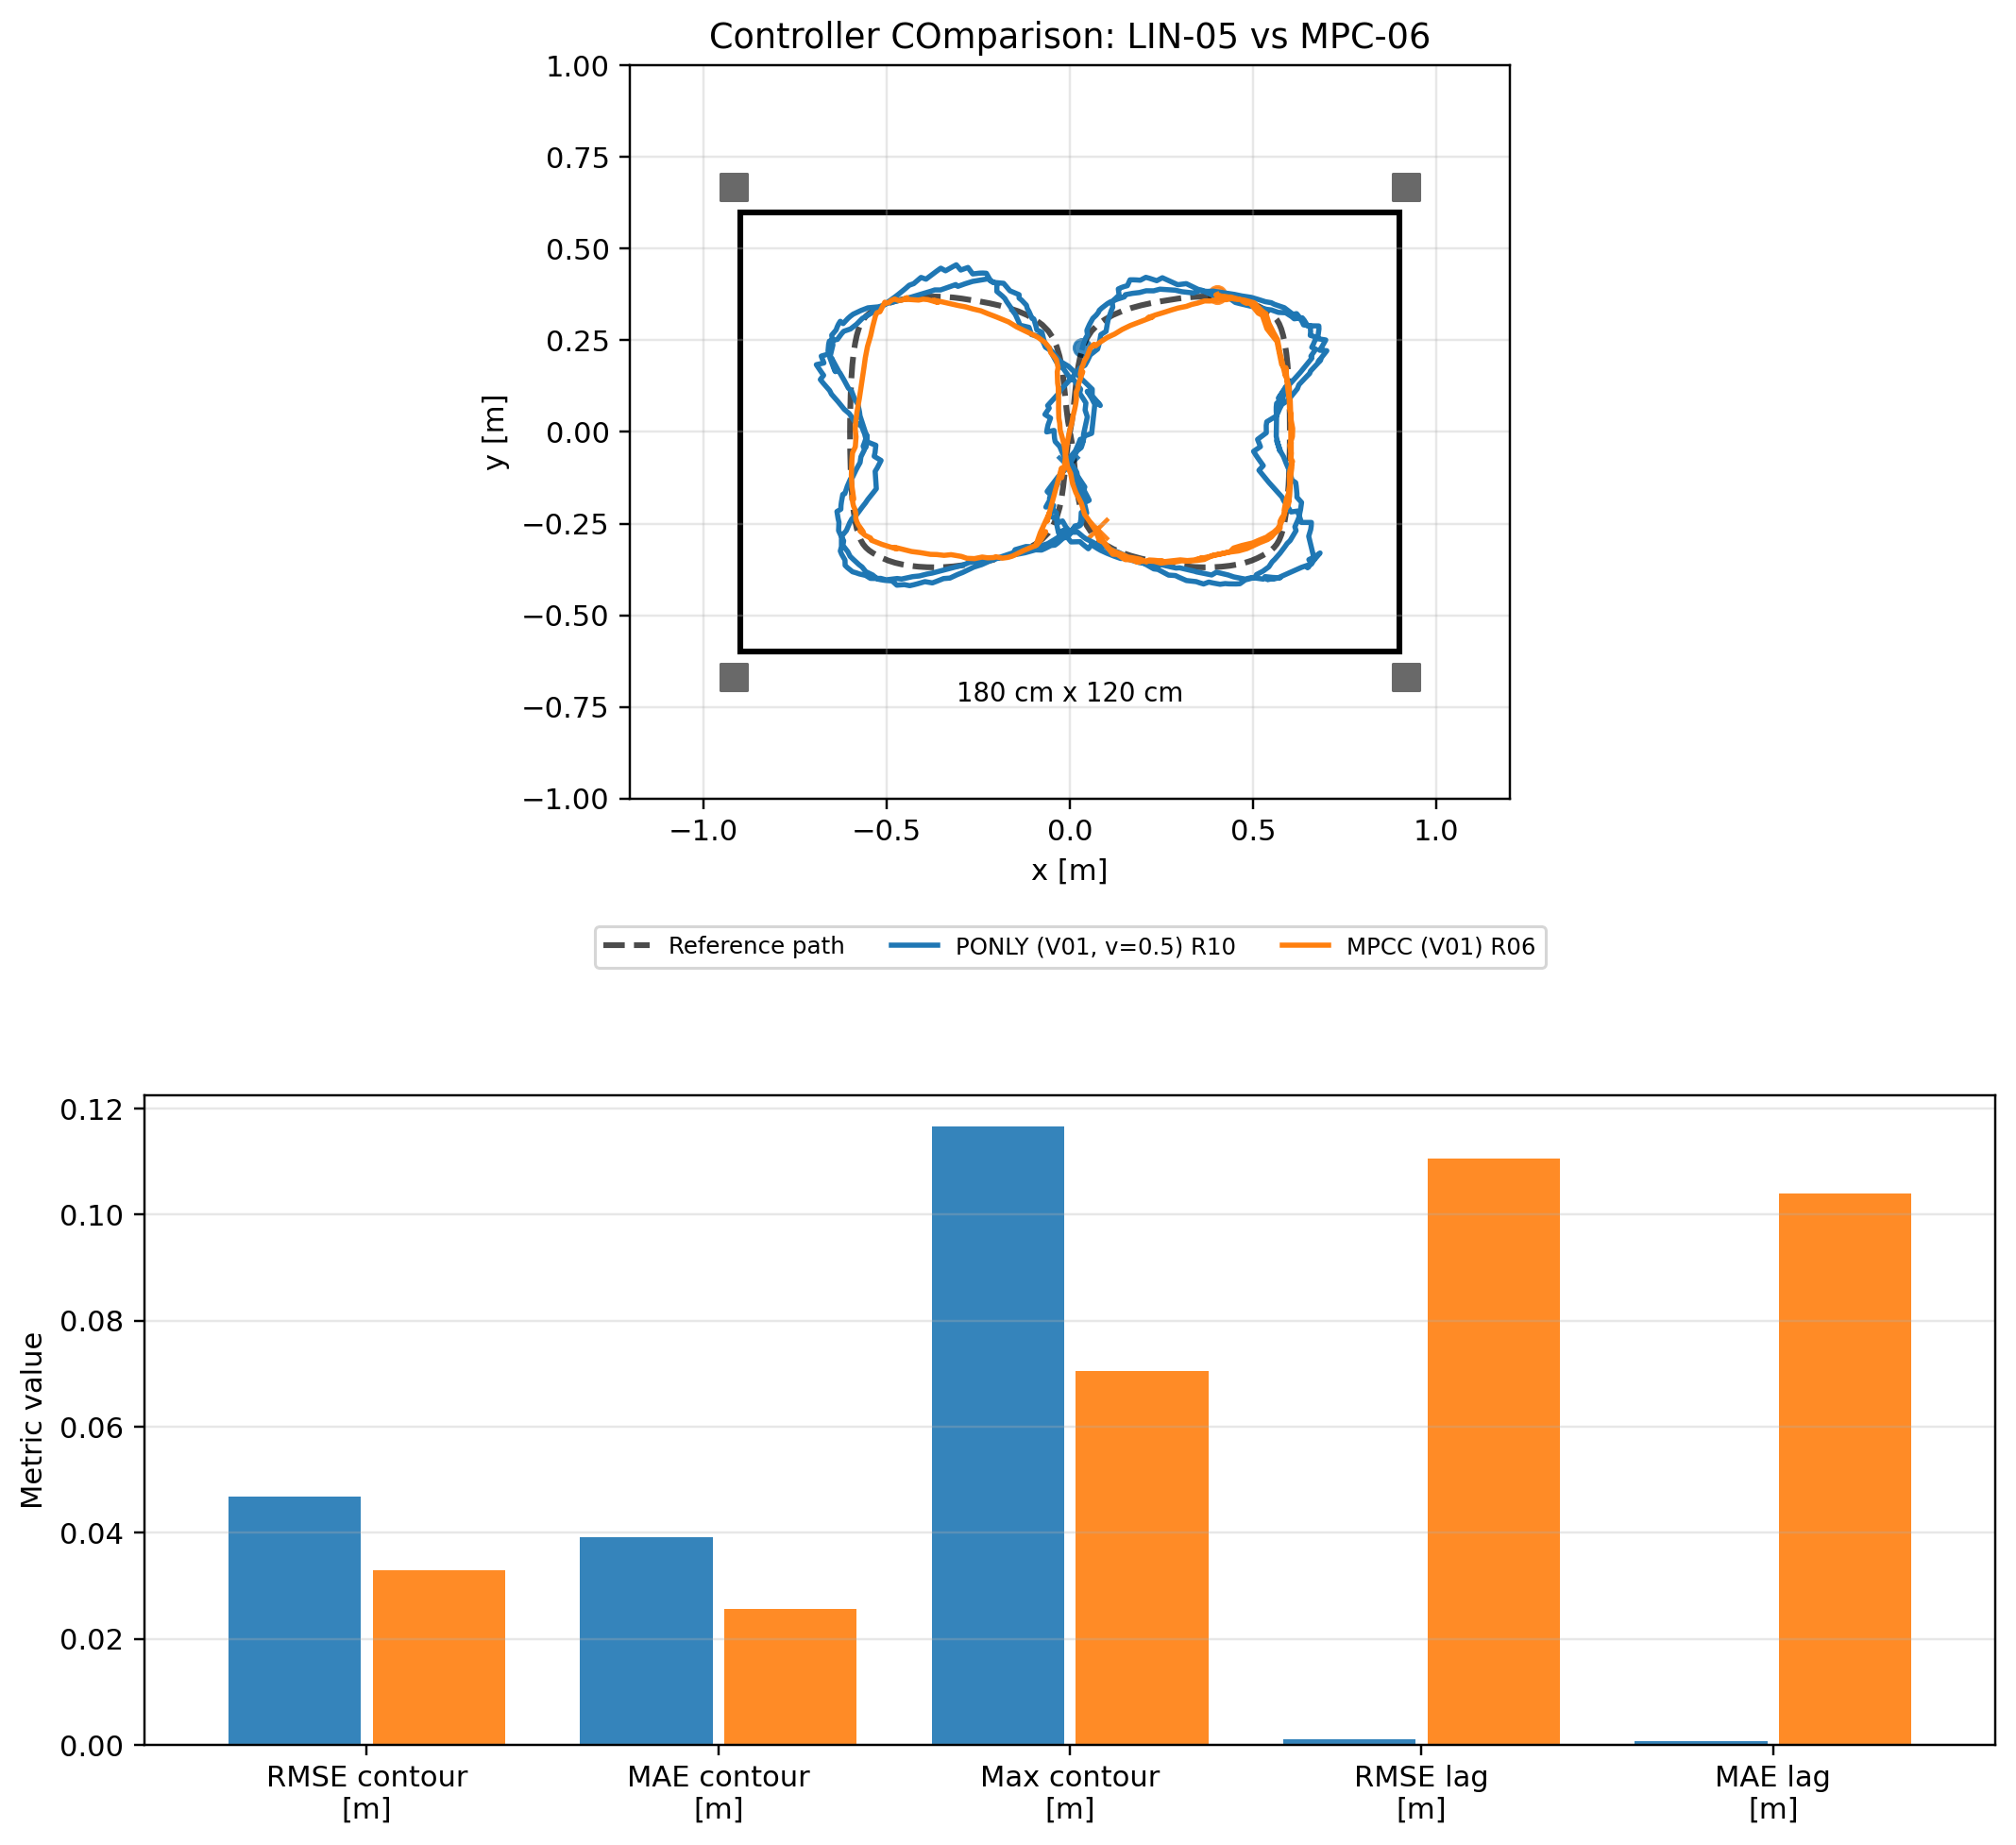
\includegraphics[width=0.95\linewidth]{IMG/controller/COMPARISON/compare_LIN05_MPC06.png}
    \caption{Common-segment comparison between the aggressive Linear Segment run
LIN-R10 and the aggressive MPCC run MPC-R06. MPC-R06 reduces the contouring error
but presents a larger lag error.}
    \label{fig:compare_lin10_mpc06}
\end{figure}


\newpage
\printbibliography[heading=bibintoc]

\end{document}